%%%%%%%%%%%%%%%%%%%%%%%%%%%%%%%%%%%%%%%%%%%%%%%%%%%%%%%%%%%%%%%%%%%%%%%%%%%
%% This file is part of the book
%%
%% Algorithmic Graph Theory
%% http://code.google.com/p/graph-theory-algorithms-book/
%%
%% Copyright (C) 2009, 2010, 2011 Minh Van Nguyen <nguyenminh2@gmail.com>
%% Copyright (C) 2010 Nathann Cohen <nathann.cohen@gmail.com>
%%
%% See the file COPYING for copying conditions.
%%%%%%%%%%%%%%%%%%%%%%%%%%%%%%%%%%%%%%%%%%%%%%%%%%%%%%%%%%%%%%%%%%%%%%%%%%%

\chapter{Random Graphs}
\label{chap:random_graphs}

A random\index{random graph} graph can be thought of as being a member
from a collection of graphs having some common properties. Recall that
Algorithm~\ref{alg:trees_forests:random_binary_tree} allows for
generating a random binary tree having at least one vertex. Fix a
positive integer $n$ and let $\cT$ be a collection of all binary trees
on $n$ vertices. It can be infeasible to generate all members of
$\cT$, so for most purposes we are only interested in randomly
generating a member of $\cT$. A binary tree of order $n$ generated in
this manner is said to be a random\index{random graph} graph.

%% \begin{itemize}
%% \item See Bollob{\'a}s~\cite{Bollobas2001}.
%%
%% \item See Gerke~et~al.~\cite{GerkeEtAl2008} for a random planar graph
%%   process.
%%
%% \item See Fusy~\cite{Fusy2009} for a linear algorithm on uniform
%%   random sampling of planar graphs.
%%
%% \item See Broutin~\cite{Broutin2007} on random trees.
%% \end{itemize}


%%%%%%%%%%%%%%%%%%%%%%%%%%%%%%%%%%%%%%%%%%%%%%%%%%%%%%%%%%%%%%%%%%%%%%%%%%%

\section{Network statistics}

Numerous real-world networks are large, having from thousands up to
millions of vertices and edges. Network statistics provide a way to
describe properties of networks without concerning ourselves with
individual vertices and edges. A network statistic should describe
essential properties of the network under consideration, provide a
means to differentiate between different classes of networks, and be
useful in network algorithms and
applications~\cite{BrinkmeierSchank2005}. In this section, we discuss
various common network statistics that can be used to describe graphs
underlying large networks.


%%%%%%%%%%%%%%%%%%%%%%%%%%%%%%%%%%%%%%%%%%%%%%%%%%%%%%%%%%%%%%%%%%%%%%%%%%%

\subsection{Degree distribution}
\label{subsec:random_graphs:degree_distribution}
\index{degree distribution}

The degree distribution of a graph $G = (V,E)$ quantifies the fraction
of vertices in $G$ having a specific degree $k$. If $v$ is any vertex
of $G$, we denote this fraction by
%%
\begin{equation}
\label{eqn:random_graphs:fraction_with_specific_degree}
p = \Pr[\deg(v) = k].
\end{equation}
%%
As indicated by the notation, we can think
of~\eqref{eqn:random_graphs:fraction_with_specific_degree} as the
probability that a vertex $v \in V$ chosen uniformly at random has
degree $k$. The \emph{degree distribution}\index{degree distribution}
of $G$ is consequently a histogram of the degrees of vertices in
$G$. Figure~\ref{fig:random_graphs:Zachary_karate_club} illustrates
the degree distribution of the
Zachary\index{network!Zachary karate club}~\cite{Zachary1977} karate
club network. The degree distributions of many real-world networks
have the same general curve as depicted in
Figure~\ref{fig:Zachary_karate_club:degree_distribution}, i.e. a peak
at low degrees followed by a tail at higher degrees. See for example
the degree distribution of the neural network in
Figure~\ref{fig:random_graphs:degree_distribution:neural_network_C_elegans},
that of a power grid network in
Figure~\ref{fig:random_graphs:degree_distribution:power_grid}, and the
degree distribution of a scientific coauthorship network in
Figure~\ref{fig:random_graphs:degree_distribution:condensed_matter_collaboration}.

\begin{figure}[!htbp]
\centering
\index{network!Zachary karate club}
\index{Zachary, Wayne W.}
%%%%%%%%%%%%%%%%%%%%%%%%%%%%%%%%%%%%%%%%%%%%%%%%%%%%%%%%%%%%%%%%%%%%%%%%%%%
%% This file is part of the book
%%
%% Algorithmic Graph Theory
%% http://code.google.com/p/graph-theory-algorithms-book/
%%
%% Copyright (C) 2009, 2010, 2011 Minh Van Nguyen <nguyenminh2@gmail.com>
%%
%% See the file COPYING for copying conditions.
%%%%%%%%%%%%%%%%%%%%%%%%%%%%%%%%%%%%%%%%%%%%%%%%%%%%%%%%%%%%%%%%%%%%%%%%%%%

\subfigure[Zachary karate club network.]{
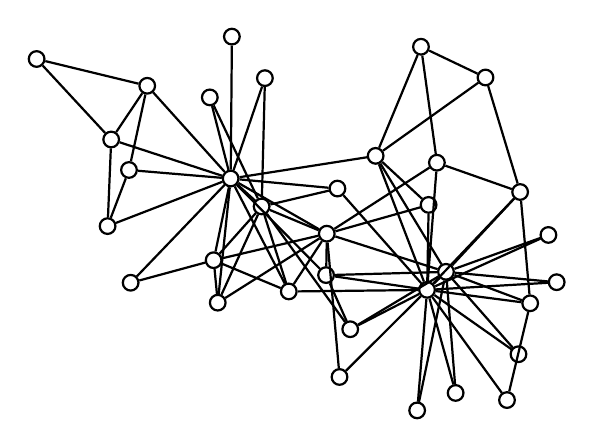
\begin{tikzpicture}
[lineDecorate/.style={-,thick},%
  nodeDecorate/.style={shape=circle,inner sep=2pt,draw,thick},
  scale=1.3,rotate=270]
%% nodes or vertices
\foreach \nodename/\x/\y in {
  0/1.77520000000000/2.16640000000000,
  1/2.04820000000000/2.46890000000000,
  2/2.31390000000000/3.10550000000000,
  3/2.57330000000000/2.00030000000000,
  4/2.24000000000000/0.964260000000000,
  5/0.869150000000000/1.35140000000000,
  6/1.39390000000000/0.999250000000000,
  7/2.98810000000000/2.04030000000000,
  8/2.71860000000000/3.09860000000000,
  9/3.71380000000000/3.23010000000000,
  10/1.69170000000000/1.17320000000000,
  11/0.388890000000000/2.17840000000000,
  12/2.79340000000000/1.18950000000000,
  13/2.87830000000000/2.73430000000000,
  14/3.49170000000000/4.97840000000000,
  15/4.04030000000000/3.98830000000000,
  16/0.607450000000000/0.270830000000000,
  17/0.794510000000000/2.50110000000000,
  18/2.78800000000000/5.35150000000000,
  19/1.87320000000000/3.20980000000000,
  20/2.32650000000000/5.27070000000000,
  21/0.982720000000000/1.96290000000000,
  22/3.87010000000000/4.36440000000000,
  23/1.90680000000000/4.99450000000000,
  24/0.487800000000000/4.02570000000000,
  25/0.788300000000000/4.65610000000000,
  26/3.93940000000000/4.86610000000000,
  27/1.62070000000000/4.18130000000000,
  28/2.03290000000000/4.10000000000000,
  29/2.99420000000000/5.09250000000000,
  30/3.24750000000000/3.33460000000000,
  31/1.55390000000000/3.58310000000000,
  32/2.68670000000000/4.27000000000000,
  33/2.86280000000000/4.08490000000000}
{
  \node (\nodename) at (\x,\y) [nodeDecorate] {};
}
%% edges or lines
\path
\foreach \startnode/\endnode in {
  0/1, 0/2, 0/3, 0/4, 0/5, 0/6, 0/7, 0/8, 0/10, 0/11, 0/12, 0/13, 0/17,
  0/19, 0/21, 0/31, 1/2, 1/3, 1/7, 1/13, 1/17, 1/19, 1/21, 1/30, 2/3,
  2/7, 2/8, 2/9, 2/13, 2/27, 2/28, 2/32, 3/7, 3/12, 3/13, 4/6, 4/10,
  5/6, 5/10, 5/16, 6/16, 8/30, 8/32, 8/33, 9/33, 13/33, 14/32, 14/33,
  15/32, 15/33, 18/32, 18/33, 19/33, 20/32, 20/33, 22/32, 22/33, 23/25,
  23/27, 23/29, 23/32, 23/33, 24/25, 24/27, 24/31, 25/31, 26/29, 26/33,
  27/33, 28/31, 28/33, 29/32, 29/33, 30/32, 30/33, 31/32, 31/33, 32/33}
{
  (\startnode) edge[lineDecorate] node {} (\endnode)
};
\end{tikzpicture}
}
%%
%%
\quad
\subfigure[Linear scaling.]{
\label{fig:Zachary_karate_club:degree_distribution}
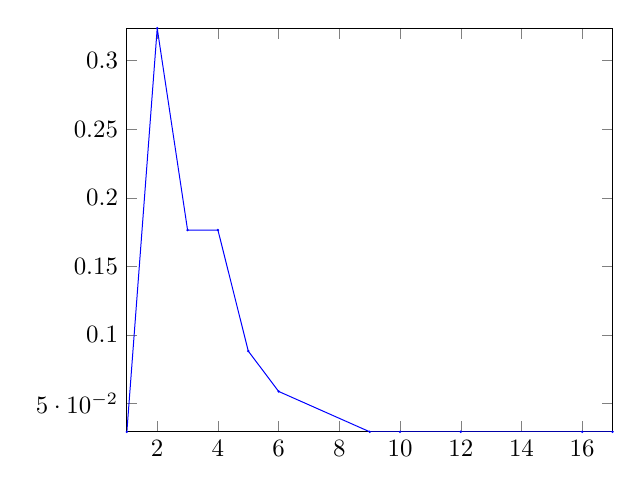
\begin{tikzpicture}
[every mark/.append style={scale=0.5},%
 scale=0.9]
\begin{axis}[%
  enlargelimits=false%
]
\addplot+[sharp plot] coordinates
{
  (1, 0.0294117647058824)  (2, 0.323529411764706)
  (3, 0.176470588235294)   (4, 0.176470588235294)
  (5, 0.0882352941176471)  (6, 0.0588235294117647)
  (9, 0.0294117647058824)  (10, 0.0294117647058824)
  (12, 0.0294117647058824) (16, 0.0294117647058824)
  (17, 0.0294117647058824)
};
\end{axis}
\end{tikzpicture}
}
%%
%%
\subfigure[Log-log scaling.]{
\label{fig:Zachary_karate_club:degree_distribution}
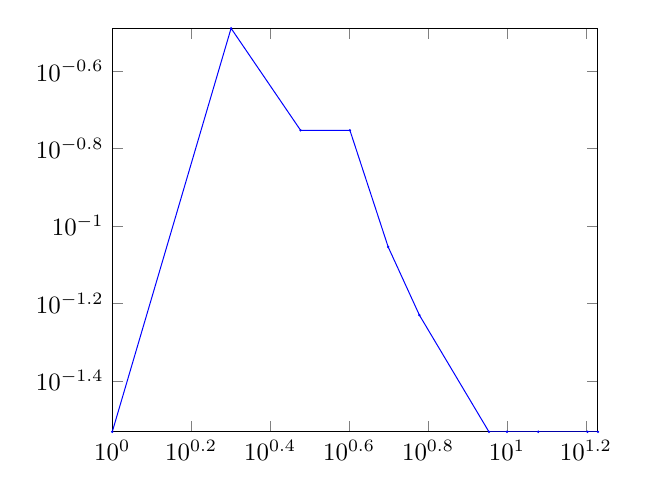
\begin{tikzpicture}
[every mark/.append style={scale=0.5},%
 scale=0.9]
\begin{loglogaxis}[%
  enlargelimits=false%
]
\addplot+[sharp plot] coordinates
{
  (1, 0.0294117647058824)  (2, 0.323529411764706)
  (3, 0.176470588235294)   (4, 0.176470588235294)
  (5, 0.0882352941176471)  (6, 0.0588235294117647)
  (9, 0.0294117647058824)  (10, 0.0294117647058824)
  (12, 0.0294117647058824) (16, 0.0294117647058824)
  (17, 0.0294117647058824)
};
\end{loglogaxis}
\end{tikzpicture}
}

\caption{The friendship network within a $34$-person karate club. This
  is more commonly known as the Zachary~\cite{Zachary1977} karate club
  network. The network is an undirected, connected, unweighted graph
  having $34$ vertices and $78$ edges. The horizontal axis represents
  degree; the vertical axis represents the probability that a vertex
  from the network has the corresponding degree.}
\label{fig:random_graphs:Zachary_karate_club}
\end{figure}

\begin{figure}[!htbp]
\centering
\index{Caenorhabditis elegans}
\index{degree distribution}
\index{network!biological}
%%%%%%%%%%%%%%%%%%%%%%%%%%%%%%%%%%%%%%%%%%%%%%%%%%%%%%%%%%%%%%%%%%%%%%%%%%%
%% This file is part of the book
%%
%% Algorithmic Graph Theory
%% http://code.google.com/p/graph-theory-algorithms-book/
%%
%% Copyright (C) 2009, 2010, 2011 Minh Van Nguyen <nguyenminh2@gmail.com>
%%
%% See the file COPYING for copying conditions.
%%%%%%%%%%%%%%%%%%%%%%%%%%%%%%%%%%%%%%%%%%%%%%%%%%%%%%%%%%%%%%%%%%%%%%%%%%%

\tikzset{every mark/.append style={scale=0.5}}
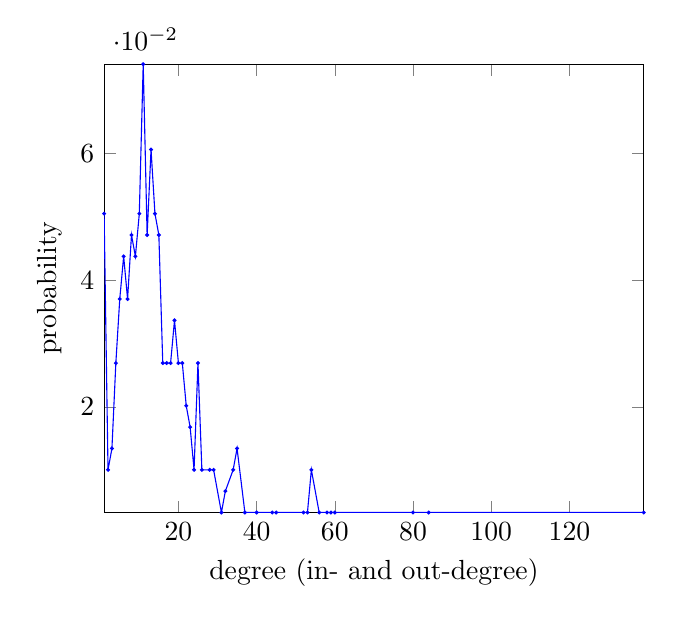
\begin{tikzpicture}[scale=1]
\begin{axis}[%
  enlargelimits=false,%
  xlabel=\text{degree (in- and out-degree)},%
  ylabel=\text{probability}%
]
\addplot+[sharp plot] coordinates
{
  (1, 0.0505050505050505)    (2, 0.0101010101010101)
  (3, 0.0134680134680135)    (4, 0.0269360269360269)
  (5, 0.0370370370370370)    (6, 0.0437710437710438)
  (7, 0.0370370370370370)    (8, 0.0471380471380471)
  (9, 0.0437710437710438)    (10, 0.0505050505050505)
  (11, 0.0740740740740741)   (12, 0.0471380471380471)
  (13, 0.0606060606060606)   (14, 0.0505050505050505)
  (15, 0.0471380471380471)   (16, 0.0269360269360269)
  (17, 0.0269360269360269)   (18, 0.0269360269360269)
  (19, 0.0336700336700337)   (20, 0.0269360269360269)
  (21, 0.0269360269360269)   (22, 0.0202020202020202)
  (23, 0.0168350168350168)   (24, 0.0101010101010101)
  (25, 0.0269360269360269)   (26, 0.0101010101010101)
  (28, 0.0101010101010101)   (29, 0.0101010101010101)
  (31, 0.00336700336700337)  (32, 0.00673400673400673)
  (34, 0.0101010101010101)   (35, 0.0134680134680135)
  (37, 0.00336700336700337)  (40, 0.00336700336700337)
  (44, 0.00336700336700337)  (45, 0.00336700336700337)
  (52, 0.00336700336700337)  (53, 0.00336700336700337)
  (54, 0.0101010101010101)   (56, 0.00336700336700337)
  (58, 0.00336700336700337)  (59, 0.00336700336700337)
  (60, 0.00336700336700337)  (80, 0.00336700336700337)
  (84, 0.00336700336700337)  (139, 0.00336700336700337)
};
\end{axis}
\end{tikzpicture}

\caption{Degree distribution of the neural network of the
  Caenorhabditis elegans. The network is a directed, not strongly
  connected, weighted graph with $297$ vertices and 2,359 edges. The
  horizontal axis represents degree; the vertical axis represents the
  probability that a vertex from the network has the corresponding
  degree. The degree distribution is derived from dataset by Watts and
  Strogatz~\cite{WattsStrogatz1998} and White et
  al.~\cite{WhiteEtAl1986}.}
\label{fig:random_graphs:degree_distribution:neural_network_C_elegans}
\end{figure}

\begin{figure}[!htbp]
\centering
\index{power grid}
\index{degree distribution}
\index{network!technological}
%%%%%%%%%%%%%%%%%%%%%%%%%%%%%%%%%%%%%%%%%%%%%%%%%%%%%%%%%%%%%%%%%%%%%%%%%%%
%% This file is part of the book
%%
%% Algorithmic Graph Theory
%% http://code.google.com/p/graph-theory-algorithms-book/
%%
%% Copyright (C) 2009, 2010, 2011 Minh Van Nguyen <nguyenminh2@gmail.com>
%%
%% See the file COPYING for copying conditions.
%%%%%%%%%%%%%%%%%%%%%%%%%%%%%%%%%%%%%%%%%%%%%%%%%%%%%%%%%%%%%%%%%%%%%%%%%%%

\begin{tikzpicture}
[every mark/.append style={scale=0.5},%
 scale=1]
\begin{axis}[%
  enlargelimits=false,%
  xlabel=\text{degree},%
  ylabel=\text{probability}%
]
\addplot+[sharp plot] coordinates
{
  (1, 0.248127909330093)      (2, 0.335154826958103)
  (3, 0.214531471362071)      (4, 0.0811576603926327)
  (5, 0.0510018214936247)     (6, 0.0277271807326453)
  (7, 0.0170006071645416)     (8, 0.00930985630439182)
  (9, 0.00546448087431694)    (10, 0.00526209269378668)
  (11, 0.00222626998583283)   (12, 0.00101194090265129)
  (13, 0.00101194090265129)   (14, 0.000607164541590771)
  (18, 0.000202388180530257)  (19, 0.000202388180530257)
};
\end{axis}
\end{tikzpicture}

\caption{Degree distribution of the Western States Power Grid of the
  United States\index{USA}. The network is an undirected, connected,
  unweighted graph with 4,941 vertices and 6,594 edges. The horizontal
  axis represents degree; the vertical axis represents the probability
  that a vertex from the network has the corresponding degree. The
  degree distribution is derived from dataset by Watts and
  Strogatz~\cite{WattsStrogatz1998}.}
\label{fig:random_graphs:degree_distribution:power_grid}
\end{figure}

\begin{figure}[!htbp]
\centering
\index{condensed matter}
\index{degree distribution}
\index{network!social}
\index{scientific collaboration}
%%%%%%%%%%%%%%%%%%%%%%%%%%%%%%%%%%%%%%%%%%%%%%%%%%%%%%%%%%%%%%%%%%%%%%%%%%%
%% This file is part of the book
%%
%% Algorithmic Graph Theory
%% http://code.google.com/p/graph-theory-algorithms-book/
%%
%% Copyright (C) 2009, 2010, 2011 Minh Van Nguyen <nguyenminh2@gmail.com>
%%
%% See the file COPYING for copying conditions.
%%%%%%%%%%%%%%%%%%%%%%%%%%%%%%%%%%%%%%%%%%%%%%%%%%%%%%%%%%%%%%%%%%%%%%%%%%%

\tikzset{every mark/.append style={scale=0.5}}
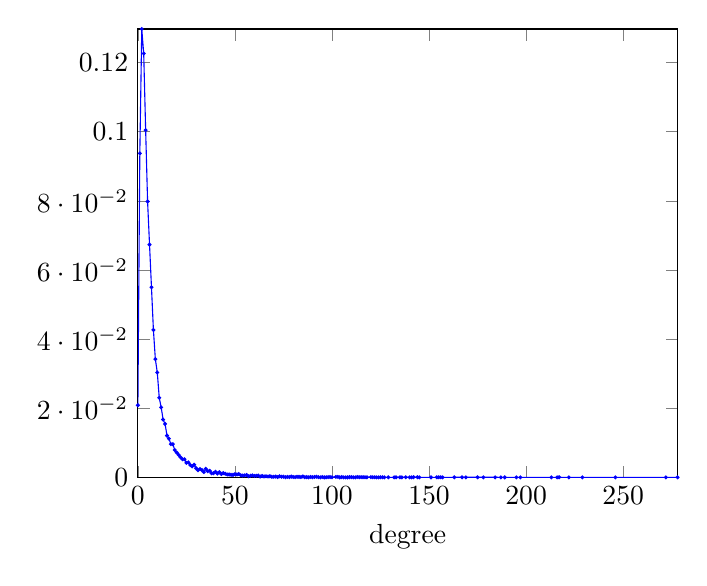
\begin{tikzpicture}[scale=1]
\begin{axis}[%
  enlargelimits=false,%
  xlabel=\text{degree}%
]
\addplot+[sharp plot] coordinates
{
  (0, 0.0208802355211396)       (1, 0.0937384033052099)
  (2, 0.129685064694093)        (3, 0.122609534647828)
  (4, 0.100467578733823)        (5, 0.0798099997526015)
  (6, 0.0673412335172292)       (7, 0.0549961653595888)
  (8, 0.0426510972019484)       (9, 0.0342148883006350)
  (10, 0.0303555082754007)      (11, 0.0230573216892205)
  (12, 0.0202617451324803)      (13, 0.0167487197248952)
  (14, 0.0154869993320301)      (15, 0.0120976720021770)
  (16, 0.0112317854580539)      (17, 0.00964845006308598)
  (18, 0.00962371044753960)     (19, 0.00794141659038620)
  (20, 0.00719922812399497)     (21, 0.00650651888869648)
  (22, 0.00583854926894437)     (23, 0.00526953811137776)
  (24, 0.00524479849583138)     (25, 0.00423047425843003)
  (26, 0.00437891195170828)     (27, 0.00358724425422430)
  (28, 0.00321615002102868)     (29, 0.00368620271640979)
  (30, 0.00267187847900844)     (31, 0.00210286732144183)
  (32, 0.00244922193909107)     (33, 0.00212760693698820)
  (34, 0.00155859577942159)     (35, 0.00249870117018382)
  (36, 0.00183073155043171)     (37, 0.00192969001261721)
  (38, 0.00121224116177235)     (39, 0.00123698077731872)
  (40, 0.00163281462606071)     (41, 0.00111328269958685)
  (42, 0.00150911654832884)     (43, 0.000989584621854976)
  (44, 0.00126172039286509)     (45, 0.00108854308404047)
  (46, 0.000865886544123104)    (47, 0.000865886544123104)
  (48, 0.000766928081937606)    (49, 0.000742188466391232)
  (50, 0.000940105390762227)    (51, 0.000865886544123104)
  (52, 0.000989584621854976)    (53, 0.000618490388659360)
  (54, 0.000544271542020237)    (55, 0.000618490388659360)
  (56, 0.000717448850844858)    (57, 0.000346354617649242)
  (58, 0.000494792310927488)    (59, 0.000593750773112986)
  (60, 0.000445313079834739)    (61, 0.000494792310927488)
  (62, 0.000544271542020237)    (63, 0.000272135771010119)
  (64, 0.000420573464288365)    (65, 0.000296875386556493)
  (66, 0.000371094233195616)    (67, 0.000272135771010119)
  (68, 0.000346354617649242)    (69, 0.000197916924370995)
  (70, 0.000222656539917370)    (71, 0.000247396155463744)
  (72, 0.000123698077731872)    (73, 0.000346354617649242)
  (74, 0.000197916924370995)    (75, 0.000222656539917370)
  (76, 0.0000742188466391232)   (77, 0.000173177308824621)
  (78, 0.0000989584621854976)   (79, 0.000247396155463744)
  (80, 0.000148437693278246)    (81, 0.0000742188466391232)
  (82, 0.000197916924370995)    (83, 0.000173177308824621)
  (84, 0.000123698077731872)    (85, 0.000272135771010119)
  (86, 0.0000742188466391232)   (87, 0.0000989584621854976)
  (88, 0.0000247396155463744)   (89, 0.000148437693278246)
  (90, 0.0000742188466391232)   (91, 0.000148437693278246)
  (92, 0.000197916924370995)    (93, 0.0000989584621854976)
  (94, 0.0000247396155463744)   (95, 0.000123698077731872)
  (96, 0.0000247396155463744)   (97, 0.0000494792310927488)
  (98, 0.0000989584621854976)   (99, 0.000123698077731872)
  (100, 0.0000494792310927488)  (102, 0.000148437693278246)
  (103, 0.000173177308824621)   (104, 0.0000247396155463744)
  (105, 0.0000989584621854976)  (106, 0.0000247396155463744)
  (107, 0.0000247396155463744)  (108, 0.0000247396155463744)
  (109, 0.0000989584621854976)  (110, 0.0000989584621854976)
  (111, 0.0000494792310927488)  (112, 0.0000247396155463744)
  (113, 0.000123698077731872)   (114, 0.0000742188466391232)
  (115, 0.0000742188466391232)  (116, 0.0000742188466391232)
  (117, 0.0000494792310927488)  (118, 0.0000494792310927488)
  (120, 0.0000989584621854976)  (121, 0.0000494792310927488)
  (122, 0.0000494792310927488)  (123, 0.0000247396155463744)
  (124, 0.0000247396155463744)  (125, 0.0000494792310927488)
  (126, 0.0000494792310927488)  (127, 0.0000247396155463744)
  (129, 0.0000494792310927488)  (132, 0.0000247396155463744)
  (133, 0.0000494792310927488)  (135, 0.0000494792310927488)
  (136, 0.0000247396155463744)  (138, 0.0000742188466391232)
  (140, 0.0000247396155463744)  (141, 0.0000247396155463744)
  (142, 0.0000742188466391232)  (144, 0.0000742188466391232)
  (145, 0.0000247396155463744)  (151, 0.0000247396155463744)
  (154, 0.0000494792310927488)  (155, 0.0000494792310927488)
  (156, 0.0000494792310927488)  (157, 0.0000247396155463744)
  (278, 0.0000247396155463744)  (163, 0.0000494792310927488)
  (167, 0.0000494792310927488)  (169, 0.0000247396155463744)
  (175, 0.0000494792310927488)  (178, 0.0000247396155463744)
  (184, 0.0000247396155463744)  (187, 0.0000247396155463744)
  (189, 0.0000247396155463744)  (195, 0.0000247396155463744)
  (197, 0.0000247396155463744)  (213, 0.0000247396155463744)
  (216, 0.0000247396155463744)  (217, 0.0000494792310927488)
  (222, 0.0000247396155463744)  (229, 0.0000247396155463744)
  (272, 0.0000247396155463744)  (246, 0.0000247396155463744)
};
\end{axis}
\end{tikzpicture}

\caption{Degree distribution of the network of coauthorships between
  scientists posting preprints on the condensed matter eprint archive
  at \url{http://arxiv.org/archive/cond-mat}. The network is a
  weighted, disconnected, undirected graph having 40,421 vertices and
  175,693 edges. The horizontal axis represents degree; the vertical
  axis represents the probability that a vertex from the coauthorship
  network has the corresponding degree. The degree distribution is
  derived from the 2005 update of the dataset by
  Newman~\cite{Newman2001b}.}
\label{fig:random_graphs:degree_distribution:condensed_matter_collaboration}
\end{figure}


%%%%%%%%%%%%%%%%%%%%%%%%%%%%%%%%%%%%%%%%%%%%%%%%%%%%%%%%%%%%%%%%%%%%%%%%%%%

\subsection{Distance statistics}

In chapter~\ref{chap:distance_connectivity} we discussed various
distance metrics such as radius, diameter, and eccentricity. To that
distance statistics collection we add the average or characteristic
distance $\cdis$, defined as the arithmetic mean of all
distances in a graph. Let $G = (V,E)$ be a simple graph with
$n = |V|$ and $m = |E|$, where $G$ can be either directed or
undirected. Then $G$ has size at most $n(n - 1)$ because for any
distinct vertex pair $u,v \in V$ we count the edge from $u$ to $v$ and
the edge from $v$ to $u$. The
\emph{characteristic distance}\index{distance!characteristic} of $G$
is defined by
\[
\cdis(G)
=
\frac{1}{n(n-1)}
\sum_{u \neq v \in V} d(u,v)
\]
where the distance function $d$ is given by
\[
d(u,v)
=
\begin{cases}
\infty, & \text{if there is no path from $u$ to $v$}, \\[4pt]
0, & \text{if $u = v$}, \\[4pt]
k, & \text{where $k$ is the length of a shortest $u$-$v$ path}.
\end{cases}
\]

If $G$ is strongly connected~(respectively, connected for the
undirected case) then our distance function is of the form
$d: V \times V \to \Z_{+} \cup \{0\}$, where the codomain is the set
of nonnegative integers. The case where $G$ is not strongly
connected~(respectively, disconnected for the undirected version)
requires special care. One way is to compute the characteristic
distance for each component and then find the average of all such
characteristic distances. Call the resulting characteristic distance
$\cdis_c$, where $c$ means component. Another way is to assign
a large number as the distance of non-existing shortest paths. If
there is no $u$-$v$ path, we let $d(u,v) = n$ because $n = |V|$ is
larger than the length of any shortest path between connected
vertices. The resulting characteristic distance is denoted
$\cdis_b$, where $b$ means big number. Furthermore denote by
$d_\kappa$ the number of pairs $(u,v)$ such that $v$ is not reachable
from $u$. For example, the Zachary~\cite{Zachary1977} karate club
network has $\cdis = 2.4082$ and $d_\kappa = 0$; the C. elegans neural
network~\cite{WattsStrogatz1998,WhiteEtAl1986} has
$\cdis_b = 71.544533$, $\cdis_c = 3.991884$, and
$d_\kappa = 20,268$; the Western States Power Grid
network~\cite{WattsStrogatz1998} has $\cdis = 18.989185$ and
$d_\kappa = 0$; and the condensed matter coauthorship
network~\cite{Newman2001b} has $\cdis_b = 7541.74656$,
$\cdis_c = 5.499329$, and $d_\kappa = 152,328,281$.

We can also define the concept of distance distribution similar to how
the degree distribution was defined in
section~\ref{subsec:random_graphs:degree_distribution}. If $\ell$ is a
positive integer with $u$ and $v$ being connected vertices in a graph
$G = (V,E)$, denote by
%%
\begin{equation}
\label{eqn:random_graphs:distance_distribution}
p
=
\Pr[d(u,v) = \ell]
\end{equation}
%%
the fraction of ordered pairs of connected vertices in $V \times V$
having distance $\ell$ between them. As is evident from the above
notation, we can think
of~\eqref{eqn:random_graphs:distance_distribution} as the probability
that a uniformly chosen connected pair $(u,v)$ of vertices in $G$ has
distance $\ell$. The
\emph{distance distribution}\index{distance distribution} of $G$ is
hence a histogram of the distances between pairs of vertices in
$G$. Figure~\ref{fig:random_graphs:distance_distribution} illustrates
distance distributions of various real-world networks.

\begin{figure}[!htbp]
\centering
%%%%%%%%%%%%%%%%%%%%%%%%%%%%%%%%%%%%%%%%%%%%%%%%%%%%%%%%%%%%%%%%%%%%%%%%%%%
%% This file is part of the book
%%
%% Algorithmic Graph Theory
%% http://code.google.com/p/graph-theory-algorithms-book/
%%
%% Copyright (C) 2009--2011 Minh Van Nguyen <nguyenminh2@gmail.com>
%%
%% See the file COPYING for copying conditions.
%%%%%%%%%%%%%%%%%%%%%%%%%%%%%%%%%%%%%%%%%%%%%%%%%%%%%%%%%%%%%%%%%%%%%%%%%%%

\documentclass{article}

\usepackage{pgfplots}
\usepackage{subfigure}
\usetikzlibrary{external}
\tikzexternalize{distance-distribution}

\begin{document}

\begin{figure}
\subfigure[Zachary karate club network~\cite{Zachary1977}.]
{
\begin{tikzpicture}
[every mark/.append style={scale=0.5},%
 scale=0.9]
\begin{axis}[%
  enlargelimits=false%
]
\addplot+[sharp plot] coordinates
{
  (1, 0.139037433155080)  (2, 0.472370766488414)
  (3, 0.244206773618538)  (4, 0.130124777183601)
  (5, 0.0142602495543672)
};
\end{axis}
\end{tikzpicture}
}
%%
%%
\quad
\subfigure[C. elegans neural network~\cite{WattsStrogatz1998,WhiteEtAl1986}.]
{
\begin{tikzpicture}
[every mark/.append style={scale=0.5},%
 scale=0.9]
\begin{axis}[%
  enlargelimits=false%
]
\addplot+[sharp plot] coordinates
{
  (1, 0.0346667849328839)     (2, 0.173954822305009)
  (3, 0.300780557033883)      (4, 0.208932056058187)
  (5, 0.0949234226243274)     (6, 0.0639081071491928)
  (7, 0.0490509136065283)     (8, 0.0293300218792502)
  (9, 0.0213174856602212)     (10, 0.0139849801904086)
  (11, 0.00671160782922358)   (12, 0.00209922535627698)
  (13, 0.000310448820294483)  (14, 0.0000295665543137603)
};
\end{axis}
\end{tikzpicture}
}
%%
%%
\subfigure[Power grid network~\cite{WattsStrogatz1998}.]
{
\begin{tikzpicture}
[every mark/.append style={scale=0.5},%
 scale=0.9]
\begin{axis}[%
  enlargelimits=false%
]
\addplot+[sharp plot] coordinates
{
  (1, 0.000540302697334621)    (2, 0.00131388440275412)
  (3, 0.00249879755200434)     (4, 0.00426965316237677)
  (5, 0.00661727411799313)     (6, 0.00946865318450018)
  (7, 0.0129893062018457)      (8, 0.0170914769994436)
  (9, 0.0216128453401965)      (10, 0.0263555296629786)
  (11, 0.0311600775794046)     (12, 0.0359045645499485)
  (13, 0.0406960842393687)     (14, 0.0453504388218222)
  (15, 0.0496812181310312)     (16, 0.0533967209837213)
  (17, 0.0559178058171443)     (18, 0.0568477262466334)
  (19, 0.0568661624169246)     (20, 0.0561867280877922)
  (21, 0.0546287487903824)     (22, 0.0524594260861158)
  (23, 0.0500720649412050)     (24, 0.0471905324939550)
  (25, 0.0435663091688401)     (26, 0.0386844932142603)
  (27, 0.0327940138984142)     (28, 0.0265576720279050)
  (29, 0.0204743913400802)     (30, 0.0150351475344285)
  (31, 0.0106571716292740)     (32, 0.00733562925107360)
  (33, 0.00497620914647087)    (34, 0.00344715415178458)
  (35, 0.00242570837911649)    (36, 0.00172742818701979)
  (37, 0.00123735381141191)    (38, 0.000847162509515112)
  (39, 0.000528831302486753)   (40, 0.000301369930360439)
  (41, 0.000164204823393779)   (42, 0.0000785790547079014)
  (43, 0.0000302353192775971)  (44, 0.0000106520095015925)
  (45, 3.60529552361591e-6)    (46, 6.55508277021075e-7)
};
\end{axis}
\end{tikzpicture}
}
%%
%%
\qquad
\subfigure[Condensed matter coauthorship network~\cite{Newman2001b}.]
{
\begin{tikzpicture}
[every mark/.append style={scale=0.5},%
 scale=0.9]
\begin{axis}[%
  enlargelimits=false%
]
\addplot+[sharp plot] coordinates
{
  (1, 0.000264366917296138)    (2, 0.00361521492316542)
  (3, 0.0352921611353204)      (4, 0.162705582489662)
  (5, 0.321747496907179)       (6, 0.285209332522791)
  (7, 0.133944826388271)       (8, 0.0424488948269472)
  (9, 0.0111017102047600)      (10, 0.00270642308054925)
  (11, 0.000694119459596421)   (12, 0.000202672325160658)
  (13, 0.0000539137395725535)  (14, 0.0000109903978185300)
  (15, 1.87787739287041e-6)    (16, 3.61130267859694e-7)
  (17, 5.26648307295387e-8)    (18, 3.00941889883078e-9)
};
\end{axis}
\end{tikzpicture}
}
\end{figure}

\end{document}

\caption{Distance distributions for various real-world networks. The
  horizontal axis represents distance and the vertical axis represents
  the probability that a uniformly chosen pair of distinct vertices
  from the network has the corresponding distance between them.}
\label{fig:random_graphs:distance_distribution}
\end{figure}


\begin{algorithm}[!htbp]
\index{algorithm!random}
\index{simple graph!random}
%%%%%%%%%%%%%%%%%%%%%%%%%%%%%%%%%%%%%%%%%%%%%%%%%%%%%%%%%%%%%%%%%%%%%%%%%%%
%% This file is part of the book
%%
%% Algorithmic Graph Theory
%% http://code.google.com/p/graph-theory-algorithms-book/
%%
%% Copyright (C) 2009--2011 Minh Van Nguyen <nguyenminh2@gmail.com>
%%
%% See the file COPYING for copying conditions.
%%%%%%%%%%%%%%%%%%%%%%%%%%%%%%%%%%%%%%%%%%%%%%%%%%%%%%%%%%%%%%%%%%%%%%%%%%%

\DontPrintSemicolon
\SetAlgoNoLine
%%
%% input
\KwIn{Positive integer $n$ and a probability $0 < p < 1$.}
%%
%% output
\KwOut{A random graph from $G(n,p)$.}
\BlankLine
%%
%% algorithm body
$G \assign \overline{K_n}$\;
$V \assign \{0, 1, \dots, n - 1\}$\;
$E \assign$ $\{2$-combinations of $V\}$\;
\For{\rm each $e \in E$}{
  $r \assign$ draw uniformly at random from interval $(0,1)$\;
  \If{$r < p$}{
    add edge $e$ to $G$\;
  }
}
\Return $G$\;

\caption{Generate a random graph in $\cG(n,p)$.}
\label{alg:random_graphs:generate_random_Gnp}
\end{algorithm}


%%%%%%%%%%%%%%%%%%%%%%%%%%%%%%%%%%%%%%%%%%%%%%%%%%%%%%%%%%%%%%%%%%%%%%%%%%%

\section{Binomial random graph model}

Fix a positive integer $n$, a probability $p$, and a vertex set
$V = \{0, 1, \dots, n - 1\}$. The
\emph{binomial}\index{random graph!binomial}~(or
\emph{Bernoulli})\index{random graph!Bernoulli} random graph model,
denoted $\cG(n,p)$ and introduced by Gilbert~\cite{Gilbert1959}, is
formally a probability\index{probability!space} space over the set of
undirected simple graphs on $n$ vertices. If $G$ is any element of the
probability space $\cG(n,p)$ and $ij$ is any edge for distinct
$i,j \in V$, then $ij$ occurs as an edge of $G$ independently with
probability $p$. In symbols, for any distinct pair $i,j \in V$ we have
\[
\Pr[ij \in E(G)]
=
p
\]
where all such events are mutually independent. Equivalently the model
$\cG(n,p)$ considers the collection of all undirected simple graphs on
$n$ vertices, each such graph having at most $\binom{n}{2}$ edges, $m$
actual edges, and an associated probability
%%
\begin{equation}
\label{eqn:random_graphs:probability_of_chosen_graph_binomial_model}
p^m (1 - p)^{\binom{n}{2} - m}.
\end{equation}
%%
Notice the latter's resemblance to the
binomial\index{binomial!distribution} distribution. By
$G \in \cG(n,p)$ we mean that $G$ is a random graph of the space
$\cG(n,p)$ and having probability
distribution $\cG(n,p)$.

To generate a random graph in $\cG(n,p)$, start with $G$ being a graph
on $n$ vertices but no edges. That is, initially $G$ is
$\overline{K_n}$, the complement of the complete\index{complete graph}
graph on $n$ vertices. Consider each of the $\binom{n}{2}$ possible
edges in some order and add it independently to $G$ with probability
$p$. See Algorithm~\ref{alg:random_graphs:generate_random_Gnp} for
pseudocode of the procedure. The runtime of
Algorithm~\ref{alg:random_graphs:generate_random_Gnp} depends on an
efficient algorithm for generating all $2$-combinations of a set of
$n$ objects. We could adapt
Algorithm~\ref{alg:tree_data_structures:generate_all_r_combinations}
to our needs or search for a more efficient algorithm; see
problem~\ref{chap:random_graphs}.\ref{prob:random_graphs:quadratic_generate_random_Gnp}
for discussion of an algorithm to generate a graph in $\cG(n,p)$ in
quadratic
time. Figure~\ref{fig:random_graphs:binomial_random_graph_25_nodes}
illustrates some random graphs from $\cG(25,p)$ with $p = i/6$ for
$i = 0, 1, \dots, 5$.

The expected number of edges of any $G \in \cG(n,p)$ is
\[
\alpha
=
\E[|E|]
=
p \cdot \binom{n}{2}
=
\frac{p \cdot n!} {2! (n - 2)!}
\]
and the expected total degree is
\[
\beta
=
\E[\#\deg]
=
2p \cdot \binom{n}{2}
=
pn(n - 1).
\]
Then the expected degree of each edge is $p(n - 1)$. From
problem~\ref{chap:introduction}.\ref{prob:introduction:number_simple_graphs}
we know that the number of undirected simple graphs on $n$ vertices is
given by
\[
2^{n(n-1) / 2}
\]
where~\eqref{eqn:random_graphs:probability_of_chosen_graph_binomial_model}
is the probability of any of these graphs being the output of the
above procedure. Let $\kappa(n,m)$ be the number of graphs from
$\cG(n,p)$ that are connected and have size $m$, and by $\Pr[G_\kappa]$
is meant the probability that $G \in \cG(n,p)$ is connected. Apply
expression~\eqref{eqn:random_graphs:probability_of_chosen_graph_binomial_model}
to see that
\[
\Pr[G_\kappa]
=
\sum_{i=n-1}^{\binom{n}{2}}
\kappa(n,i) \cdot p^i (1 - p)^{\binom{n}{2} - i}
\]
where $n - 1$ is the least number of edges of any undirected connected
graph on $n$ vertices, i.e. the size of any spanning tree of a
connected graph in $\cG(n,p)$. Similarly define $\Pr[\kappa_{ij}]$ to
be the probability that two distinct vertices $i,j$ of
$G \in \cG(n,p)$ are connected. Gilbert~\cite{Gilbert1959} showed that
as $n \to \infty$, the probabilities $\Pr[G_\kappa]$ and
$\Pr[\kappa_{ij}]$ approach
\[
\Pr[G_\kappa] \to 1 - n(1 - p)^{n-1}
\]
and
\[
\Pr[\kappa_{ij}] \to 1 - 2(1 - p)^{n-1}.
\]

\begin{figure}[!htbp]
\centering
\index{binomial!random graph}
%%%%%%%%%%%%%%%%%%%%%%%%%%%%%%%%%%%%%%%%%%%%%%%%%%%%%%%%%%%%%%%%%%%%%%%%%%%
%% This file is part of the book
%%
%% Algorithmic Graph Theory
%% http://code.google.com/p/graph-theory-algorithms-book/
%%
%% Copyright (C) 2009, 2010, 2011 Minh Van Nguyen <nguyenminh2@gmail.com>
%%
%% See the file COPYING for copying conditions.
%%%%%%%%%%%%%%%%%%%%%%%%%%%%%%%%%%%%%%%%%%%%%%%%%%%%%%%%%%%%%%%%%%%%%%%%%%%

\documentclass{article}

\usepackage{subfigure}
\usepackage{tikz}
\usetikzlibrary{external}
\tikzexternalize{binomial-random-graphs-25-nodes}

\begin{document}

\begin{figure}
\subfigure[$p = 0$;
  $\alpha = 0$, $|E| = 0$;
  $\beta = 0$, $\#\deg = 0$]{
\begin{tikzpicture}
[lineDecorate/.style={-,thick},%
  nodeDecorate/.style={shape=circle,inner sep=2pt,draw,thick},
  scale=3.4]
%% nodes or vertices
\foreach \nodename/\x/\y in {
  0/1.00000000000000/0.000000000000000,
  1/0.968583161128631/0.248689887164855,
  2/0.876306680043864/0.481753674101715,
  3/0.728968627421412/0.684547105928689,
  4/0.535826794978997/0.844327925502015,
  5/0.309016994374947/0.951056516295154,
  6/0.0627905195293135/0.998026728428272,
  7/-0.187381314585725/0.982287250728689,
  8/-0.425779291565073/0.904827052466019,
  9/-0.637423989748690/0.770513242775789,
  10/-0.809016994374947/0.587785252292473,
  11/-0.929776485888251/0.368124552684678,
  12/-0.992114701314478/0.125333233564305,
  13/-0.992114701314478/-0.125333233564304,
  14/-0.929776485888251/-0.368124552684678,
  15/-0.809016994374947/-0.587785252292473,
  16/-0.637423989748690/-0.770513242775789,
  17/-0.425779291565072/-0.904827052466020,
  18/-0.187381314585725/-0.982287250728689,
  19/0.0627905195293128/-0.998026728428272,
  20/0.309016994374947/-0.951056516295154,
  21/0.535826794978996/-0.844327925502016,
  22/0.728968627421411/-0.684547105928689,
  23/0.876306680043864/-0.481753674101715,
  24/0.968583161128631/-0.248689887164855}
{
  \node (\nodename) at (\x,\y) [nodeDecorate] {};
}
\end{tikzpicture}
}
%%
%%
\qquad
\subfigure[$p = 1/6$;
  $\alpha = 50$, $|E| = 44$;
  $\beta = 100$, $\#\deg = 88$]{
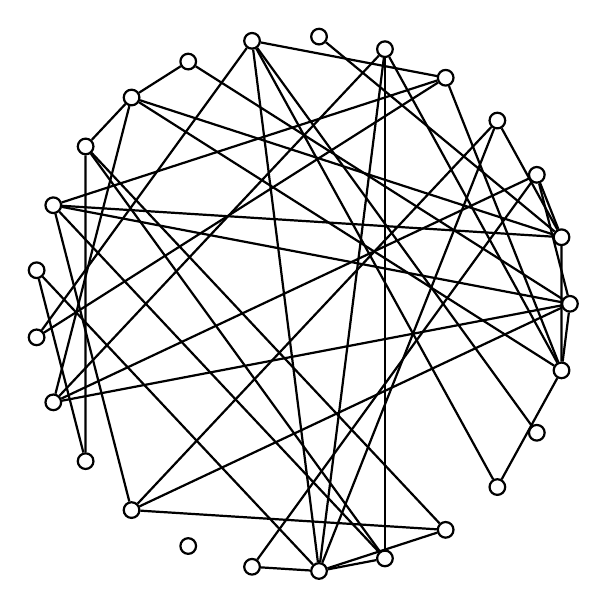
\begin{tikzpicture}
[lineDecorate/.style={-,thick},%
  nodeDecorate/.style={shape=circle,inner sep=2pt,draw,thick},
  scale=3.4]
%% nodes or vertices
\foreach \nodename/\x/\y in {
  0/1.00000000000000/0.000000000000000,
  1/0.968583161128631/0.248689887164855,
  2/0.876306680043864/0.481753674101715,
  3/0.728968627421412/0.684547105928689,
  4/0.535826794978997/0.844327925502015,
  5/0.309016994374947/0.951056516295154,
  6/0.0627905195293135/0.998026728428272,
  7/-0.187381314585725/0.982287250728689,
  8/-0.425779291565073/0.904827052466019,
  9/-0.637423989748690/0.770513242775789,
  10/-0.809016994374947/0.587785252292473,
  11/-0.929776485888251/0.368124552684678,
  12/-0.992114701314478/0.125333233564305,
  13/-0.992114701314478/-0.125333233564304,
  14/-0.929776485888251/-0.368124552684678,
  15/-0.809016994374947/-0.587785252292473,
  16/-0.637423989748690/-0.770513242775789,
  17/-0.425779291565072/-0.904827052466020,
  18/-0.187381314585725/-0.982287250728689,
  19/0.0627905195293128/-0.998026728428272,
  20/0.309016994374947/-0.951056516295154,
  21/0.535826794978996/-0.844327925502016,
  22/0.728968627421411/-0.684547105928689,
  23/0.876306680043864/-0.481753674101715,
  24/0.968583161128631/-0.248689887164855}
{
  \node (\nodename) at (\x,\y) [nodeDecorate] {};
}
%% edges or lines
\path
\foreach \startnode/\endnode in {
  0/2, 0/8, 0/11, 0/14, 0/16, 0/24, 1/2, 1/3, 1/6, 1/9, 1/11, 1/24,
  2/14, 2/18, 3/16, 3/19, 4/7, 4/11, 4/13, 4/24, 5/14, 5/19, 5/20, 5/24,
  7/13, 7/19, 7/22, 7/23, 8/9, 9/10, 9/14, 9/24, 10/15, 10/20, 10/21,
  11/16, 11/20, 12/15, 12/19, 16/21, 18/19, 19/20, 19/21, 22/24}
{
  (\startnode) edge[lineDecorate] node {} (\endnode)
};
\end{tikzpicture}
}
%%
%%
\subfigure[$p = 1/3$;
  $\alpha = 100$, $|E| = 108$;
  $\beta = 200$, $\#\deg = 212$]{
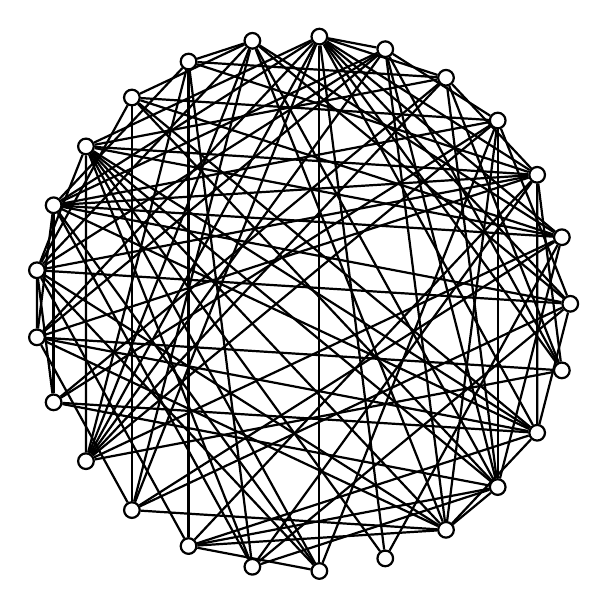
\begin{tikzpicture}
[lineDecorate/.style={-,thick},%
  nodeDecorate/.style={shape=circle,inner sep=2pt,draw,thick},
  scale=3.4]
%% nodes or vertices
\foreach \nodename/\x/\y in {
  0/1.00000000000000/0.000000000000000,
  1/0.968583161128631/0.248689887164855,
  2/0.876306680043864/0.481753674101715,
  3/0.728968627421412/0.684547105928689,
  4/0.535826794978997/0.844327925502015,
  5/0.309016994374947/0.951056516295154,
  6/0.0627905195293135/0.998026728428272,
  7/-0.187381314585725/0.982287250728689,
  8/-0.425779291565073/0.904827052466019,
  9/-0.637423989748690/0.770513242775789,
  10/-0.809016994374947/0.587785252292473,
  11/-0.929776485888251/0.368124552684678,
  12/-0.992114701314478/0.125333233564305,
  13/-0.992114701314478/-0.125333233564304,
  14/-0.929776485888251/-0.368124552684678,
  15/-0.809016994374947/-0.587785252292473,
  16/-0.637423989748690/-0.770513242775789,
  17/-0.425779291565072/-0.904827052466020,
  18/-0.187381314585725/-0.982287250728689,
  19/0.0627905195293128/-0.998026728428272,
  20/0.309016994374947/-0.951056516295154,
  21/0.535826794978996/-0.844327925502016,
  22/0.728968627421411/-0.684547105928689,
  23/0.876306680043864/-0.481753674101715,
  24/0.968583161128631/-0.248689887164855}
{
  \node (\nodename) at (\x,\y) [nodeDecorate] {};
}
%% edges or lines
\path
\foreach \startnode/\endnode in {
  0/3, 0/6, 0/7, 0/11, 0/12, 0/16, 0/18, 0/23, 1/6, 1/7, 1/9, 1/10,
  1/11, 1/15, 1/16, 1/20, 1/22, 2/4, 2/6, 2/8, 2/10, 2/11, 2/12, 2/13,
  2/17, 2/18, 2/23, 2/24, 3/5, 3/9, 3/11, 3/14, 3/15, 3/19, 3/21, 3/22,
  4/6, 4/8, 4/10, 4/14, 4/15, 4/22, 4/24, 5/6, 5/11, 5/12, 5/13, 5/15,
  5/21, 5/22, 5/24, 6/10, 6/11, 6/13, 6/15, 6/16, 6/19, 6/20, 6/23,
  6/24, 7/8, 7/9, 7/12, 7/15, 7/16, 7/21, 7/22, 8/11, 8/15, 8/17, 8/18,
  9/12, 9/16, 9/22, 9/23, 10/12, 10/15, 10/18, 10/19, 10/20, 10/21,
  10/22, 10/23, 11/13, 11/14, 11/18, 11/19, 11/23, 12/13, 12/14, 12/17,
  12/19, 12/21, 13/16, 13/21, 13/23, 13/24, 14/22, 14/23, 15/24, 16/21,
  17/19, 17/21, 17/22, 17/23, 18/22, 21/22, 21/23}
{
  (\startnode) edge[lineDecorate] node {} (\endnode)
};
\end{tikzpicture}
}
%%
%%
\qquad
\subfigure[$p = 1/2$;
  $\alpha = 150$, $|E| = 156$;
  $\beta = 300$, $\#\deg = 312$]{
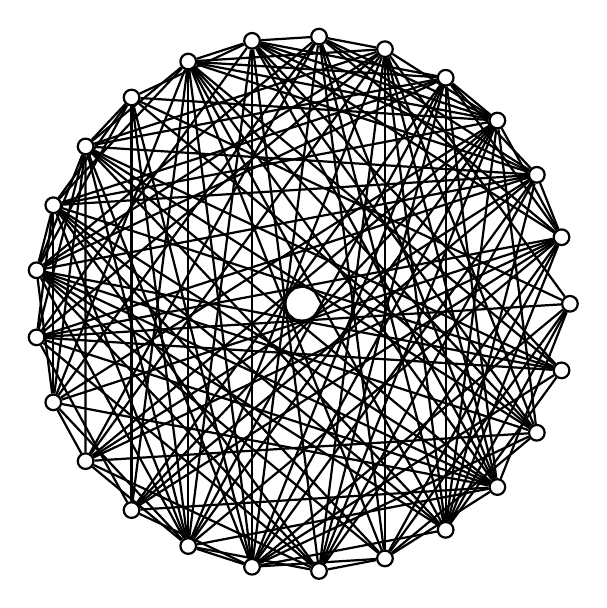
\begin{tikzpicture}
[lineDecorate/.style={-,thick},%
  nodeDecorate/.style={shape=circle,inner sep=2pt,draw,thick},
  scale=3.4]
%% nodes or vertices
\foreach \nodename/\x/\y in {
  0/1.00000000000000/0.000000000000000,
  1/0.968583161128631/0.248689887164855,
  2/0.876306680043864/0.481753674101715,
  3/0.728968627421412/0.684547105928689,
  4/0.535826794978997/0.844327925502015,
  5/0.309016994374947/0.951056516295154,
  6/0.0627905195293135/0.998026728428272,
  7/-0.187381314585725/0.982287250728689,
  8/-0.425779291565073/0.904827052466019,
  9/-0.637423989748690/0.770513242775789,
  10/-0.809016994374947/0.587785252292473,
  11/-0.929776485888251/0.368124552684678,
  12/-0.992114701314478/0.125333233564305,
  13/-0.992114701314478/-0.125333233564304,
  14/-0.929776485888251/-0.368124552684678,
  15/-0.809016994374947/-0.587785252292473,
  16/-0.637423989748690/-0.770513242775789,
  17/-0.425779291565072/-0.904827052466020,
  18/-0.187381314585725/-0.982287250728689,
  19/0.0627905195293128/-0.998026728428272,
  20/0.309016994374947/-0.951056516295154,
  21/0.535826794978996/-0.844327925502016,
  22/0.728968627421411/-0.684547105928689,
  23/0.876306680043864/-0.481753674101715,
  24/0.968583161128631/-0.248689887164855}
{
  \node (\nodename) at (\x,\y) [nodeDecorate] {};
}
%% edges or lines
\path
\foreach \startnode/\endnode in {
  0/5, 0/9, 0/13, 0/18, 0/20, 0/21, 0/22, 1/2, 1/3, 1/4, 1/6, 1/7, 1/13,
  1/14, 1/15, 1/16, 1/17, 1/19, 1/20, 1/21, 2/4, 2/6, 2/7, 2/8, 2/10,
  2/11, 2/12, 2/13, 2/15, 2/16, 2/18, 2/19, 2/21, 3/4, 3/5, 3/6, 3/7,
  3/8, 3/9, 3/11, 3/14, 3/15, 3/16, 3/17, 3/18, 3/19, 3/21, 3/23, 4/7,
  4/8, 4/10, 4/11, 4/12, 4/16, 4/17, 4/18, 4/19, 4/21, 4/22, 5/6, 5/8,
  5/10, 5/12, 5/13, 5/15, 5/17, 5/19, 5/20, 5/21, 5/22, 5/23, 6/7, 6/12,
  6/14, 6/15, 6/18, 6/20, 6/21, 6/22, 7/8, 7/9, 7/13, 7/17, 7/18, 7/19,
  7/22, 7/23, 7/24, 8/10, 8/11, 8/14, 8/16, 8/17, 8/18, 8/20, 8/21,
  8/22, 8/23, 8/24, 9/10, 9/11, 9/12, 9/16, 9/17, 9/18, 9/23, 10/12,
  10/13, 10/14, 10/15, 10/17, 10/18, 10/21, 10/22, 10/23, 10/24, 11/12,
  11/13, 11/14, 11/17, 11/19, 11/20, 11/21, 11/22, 11/24, 12/14, 12/17,
  12/19, 12/20, 12/21, 12/22, 12/23, 12/24, 13/16, 13/19, 13/22, 13/24,
  14/15, 14/17, 14/22, 15/17, 15/19, 15/23, 16/18, 16/22, 17/18, 17/19,
  17/22, 18/20, 18/21, 18/23, 18/24, 19/20, 20/22, 20/23, 21/24}
{
  (\startnode) edge[lineDecorate] node {} (\endnode)
};
\end{tikzpicture}
}
%%
%%
\subfigure[$p = 2/3$;
  $\alpha = 200$, $|E| = 185$;
  $\beta = 400$, $\#\deg = 370$]{
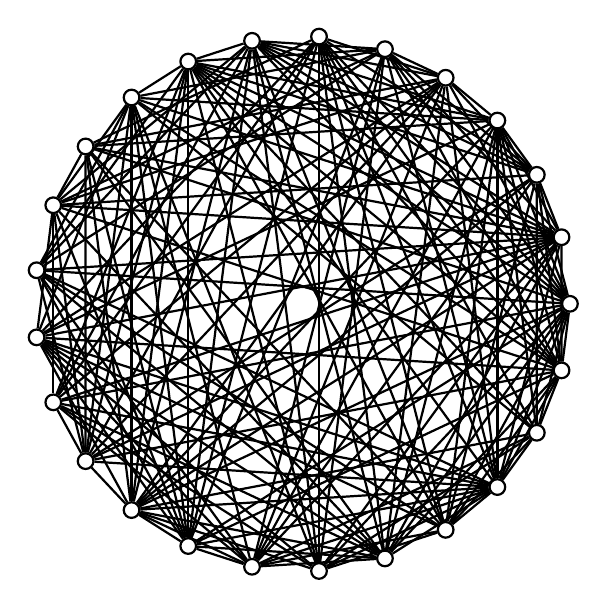
\begin{tikzpicture}
[lineDecorate/.style={-,thick},%
  nodeDecorate/.style={shape=circle,inner sep=2pt,draw,thick},
  scale=3.4]
%% nodes or vertices
\foreach \nodename/\x/\y in {
  0/1.00000000000000/0.000000000000000,
  1/0.968583161128631/0.248689887164855,
  2/0.876306680043864/0.481753674101715,
  3/0.728968627421412/0.684547105928689,
  4/0.535826794978997/0.844327925502015,
  5/0.309016994374947/0.951056516295154,
  6/0.0627905195293135/0.998026728428272,
  7/-0.187381314585725/0.982287250728689,
  8/-0.425779291565073/0.904827052466019,
  9/-0.637423989748690/0.770513242775789,
  10/-0.809016994374947/0.587785252292473,
  11/-0.929776485888251/0.368124552684678,
  12/-0.992114701314478/0.125333233564305,
  13/-0.992114701314478/-0.125333233564304,
  14/-0.929776485888251/-0.368124552684678,
  15/-0.809016994374947/-0.587785252292473,
  16/-0.637423989748690/-0.770513242775789,
  17/-0.425779291565072/-0.904827052466020,
  18/-0.187381314585725/-0.982287250728689,
  19/0.0627905195293128/-0.998026728428272,
  20/0.309016994374947/-0.951056516295154,
  21/0.535826794978996/-0.844327925502016,
  22/0.728968627421411/-0.684547105928689,
  23/0.876306680043864/-0.481753674101715,
  24/0.968583161128631/-0.248689887164855}
{
  \node (\nodename) at (\x,\y) [nodeDecorate] {};
}
%% edges or lines
\path
\foreach \startnode/\endnode in {
  0/2, 0/3, 0/4, 0/5, 0/6, 0/7, 0/8, 0/10, 0/12, 0/14, 0/16, 0/17, 0/19,
  0/20, 0/21, 0/22, 0/23, 0/24, 1/2, 1/3, 1/5, 1/7, 1/8, 1/9, 1/10,
  1/11, 1/12, 1/13, 1/14, 1/15, 1/16, 1/18, 1/19, 1/20, 1/22, 1/24, 2/3,
  2/4, 2/5, 2/6, 2/7, 2/8, 2/11, 2/15, 2/16, 2/18, 2/21, 2/23, 2/24,
  3/4, 3/7, 3/8, 3/9, 3/10, 3/13, 3/16, 3/18, 3/20, 3/21, 3/22, 3/23,
  3/24, 4/5, 4/6, 4/7, 4/10, 4/11, 4/13, 4/14, 4/15, 4/16, 4/18, 4/20,
  4/22, 5/7, 5/8, 5/9, 5/11, 5/12, 5/17, 5/18, 5/19, 5/22, 5/24, 6/10,
  6/13, 6/14, 6/15, 6/17, 6/19, 6/20, 6/21, 6/22, 6/23, 6/24, 7/8, 7/11,
  7/12, 7/14, 7/16, 7/17, 7/19, 7/20, 7/21, 7/24, 8/9, 8/12, 8/14, 8/15,
  8/16, 8/17, 8/19, 8/21, 8/22, 8/23, 8/24, 9/11, 9/12, 9/13, 9/15,
  9/16, 9/17, 9/18, 9/19, 9/23, 9/24, 10/11, 10/15, 10/16, 10/17, 10/20,
  10/21, 11/13, 11/14, 11/15, 11/17, 11/20, 11/24, 12/15, 12/17, 12/18,
  12/20, 12/21, 12/22, 13/16, 13/17, 13/18, 13/19, 13/20, 13/21, 13/22,
  13/24, 14/15, 14/18, 14/19, 14/20, 14/22, 15/16, 15/22, 15/24, 16/17,
  16/18, 16/19, 16/20, 16/22, 16/23, 17/18, 17/20, 17/22, 17/24, 18/20,
  18/21, 18/22, 18/23, 19/21, 19/22, 19/23, 20/22, 20/24, 21/22, 21/23,
  21/24, 22/23, 22/24, 23/24}
{
  (\startnode) edge[lineDecorate] node {} (\endnode)
};
\end{tikzpicture}
}
%%
%%
\qquad
\subfigure[$p = 5/6$;
  $\alpha = 250$, $|E| = 255$;
  $\beta = 500$, $\#\deg = 510$]{
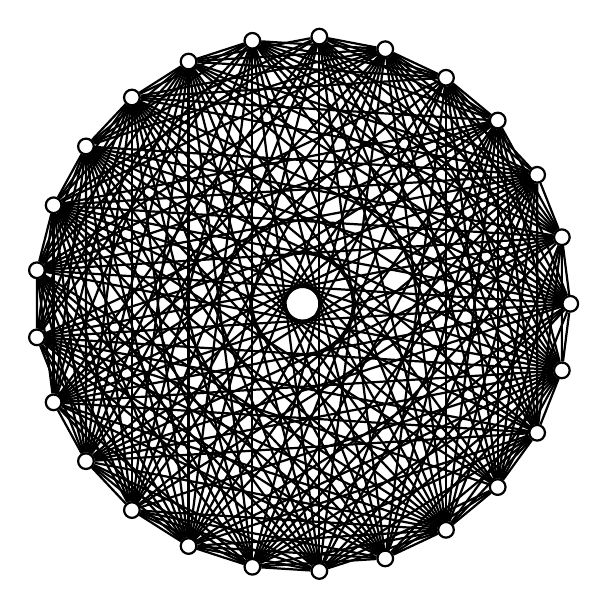
\begin{tikzpicture}
[lineDecorate/.style={-,thick},%
  nodeDecorate/.style={shape=circle,inner sep=2pt,draw,thick},
  scale=3.4]
%% nodes or vertices
\foreach \nodename/\x/\y in {
  0/1.00000000000000/0.000000000000000,
  1/0.968583161128631/0.248689887164855,
  2/0.876306680043864/0.481753674101715,
  3/0.728968627421412/0.684547105928689,
  4/0.535826794978997/0.844327925502015,
  5/0.309016994374947/0.951056516295154,
  6/0.0627905195293135/0.998026728428272,
  7/-0.187381314585725/0.982287250728689,
  8/-0.425779291565073/0.904827052466019,
  9/-0.637423989748690/0.770513242775789,
  10/-0.809016994374947/0.587785252292473,
  11/-0.929776485888251/0.368124552684678,
  12/-0.992114701314478/0.125333233564305,
  13/-0.992114701314478/-0.125333233564304,
  14/-0.929776485888251/-0.368124552684678,
  15/-0.809016994374947/-0.587785252292473,
  16/-0.637423989748690/-0.770513242775789,
  17/-0.425779291565072/-0.904827052466020,
  18/-0.187381314585725/-0.982287250728689,
  19/0.0627905195293128/-0.998026728428272,
  20/0.309016994374947/-0.951056516295154,
  21/0.535826794978996/-0.844327925502016,
  22/0.728968627421411/-0.684547105928689,
  23/0.876306680043864/-0.481753674101715,
  24/0.968583161128631/-0.248689887164855}
{
  \node (\nodename) at (\x,\y) [nodeDecorate] {};
}
%% edges or lines
\path
\foreach \startnode/\endnode in {
  0/1, 0/3, 0/4, 0/5, 0/6, 0/7, 0/8, 0/9, 0/10, 0/11, 0/12, 0/13, 0/14,
  0/15, 0/17, 0/18, 0/19, 0/22, 0/24, 1/2, 1/3, 1/4, 1/5, 1/6, 1/7, 1/8,
  1/10, 1/11, 1/12, 1/13, 1/14, 1/15, 1/16, 1/18, 1/21, 1/22, 1/23,
  1/24, 2/4, 2/5, 2/7, 2/8, 2/9, 2/10, 2/11, 2/12, 2/13, 2/14, 2/15,
  2/16, 2/17, 2/18, 2/19, 2/20, 2/21, 2/22, 2/23, 3/4, 3/5, 3/6, 3/7,
  3/9, 3/11, 3/12, 3/13, 3/14, 3/15, 3/17, 3/18, 3/19, 3/20, 3/21, 3/22,
  3/23, 3/24, 4/5, 4/6, 4/7, 4/8, 4/9, 4/12, 4/14, 4/16, 4/17, 4/18,
  4/20, 4/21, 4/22, 4/23, 4/24, 5/6, 5/7, 5/8, 5/9, 5/10, 5/11, 5/12,
  5/14, 5/15, 5/16, 5/17, 5/18, 5/19, 5/21, 5/22, 5/23, 5/24, 6/8, 6/10,
  6/11, 6/14, 6/15, 6/16, 6/17, 6/19, 6/20, 6/21, 6/22, 6/23, 6/24, 7/8,
  7/9, 7/10, 7/12, 7/13, 7/15, 7/16, 7/17, 7/18, 7/19, 7/20, 7/21, 7/23,
  7/24, 8/9, 8/10, 8/11, 8/12, 8/13, 8/14, 8/15, 8/16, 8/17, 8/18, 8/19,
  8/20, 8/21, 8/22, 8/24, 9/10, 9/11, 9/12, 9/13, 9/14, 9/15, 9/16,
  9/17, 9/18, 9/19, 9/20, 9/21, 9/22, 9/23, 9/24, 10/11, 10/12, 10/13,
  10/14, 10/15, 10/16, 10/17, 10/18, 10/19, 10/20, 10/21, 10/22, 10/23,
  10/24, 11/12, 11/13, 11/14, 11/15, 11/16, 11/17, 11/18, 11/19, 11/20,
  11/21, 11/22, 11/23, 11/24, 12/13, 12/14, 12/15, 12/16, 12/17, 12/18,
  12/19, 12/20, 12/21, 12/24, 13/15, 13/16, 13/17, 13/19, 13/20, 13/21,
  13/22, 13/23, 13/24, 14/15, 14/17, 14/18, 14/20, 14/21, 14/23, 14/24,
  15/16, 15/17, 15/18, 15/19, 15/21, 15/23, 15/24, 16/17, 16/18, 16/19,
  16/20, 16/21, 16/24, 17/18, 17/19, 17/20, 17/21, 17/23, 17/24, 18/19,
  18/20, 18/21, 18/23, 18/24, 19/21, 19/22, 19/23, 19/24, 20/21, 20/22,
  20/23, 20/24, 21/22, 21/23, 21/24, 22/23, 22/24, 23/24}
{
  (\startnode) edge[lineDecorate] node {} (\endnode)
};
\end{tikzpicture}
}
\end{figure}

\end{document}

\caption{Binomial random graphs $\cG(25,p)$ for various values of $p$.}
\label{fig:random_graphs:binomial_random_graph_25_nodes}
\end{figure}


%%%%%%%%%%%%%%%%%%%%%%%%%%%%%%%%%%%%%%%%%%%%%%%%%%%%%%%%%%%%%%%%%%%%%%%%%%%

\subsubsection{Efficient generation of sparse $G \in \cG(n,p)$}

The techniques discussed so
far~(Algorithms~\ref{alg:random_graphs:generate_random_Gnp}
and~\ref{alg:random_graphs:quadratic_generate_random_Gnp}) for
generating a random graph from $\cG(n,p)$ can be unsuitable when the
number of vertices $n$ is in the hundreds of thousands or millions. In
many applications of $\cG(n,p)$ we are only interested in
sparse\index{sparse graph} random graphs. A linear time algorithm to
generate a random sparse graph from $\cG(n,p)$ is presented in
Batagelj\index{Batagelj, Vladimir} and
Brandes\index{Brandes, Ulrik}~\cite{BatageljBrandes2005}.

The Batagelj-Brandes\index{Batagelj-Brandes algorithm} algorithm for
generating a random sparse graph $G \in \cG(n,p)$ uses what is known as
a geometric method to skip over certain edges. Fix a probability
$0 < p < 1$ that an edge will be in the resulting random sparse graph
$G$. If $e$ is an edge of $G$, we can consider the events leading up
to the choice of $e$ as
\[
e_1, e_2, \dots, e_k
\]
where in the $i$-th trial the event $e_i$ is a failure, for
$1 \leq i < k$, but the event $e_k$ is the first success after
$k - 1$ successive failures. In probabilistic terms, we perform a
series of independent trials each having success probability $p$ and
stop when the first success occurs. Letting $X$ be the number of
trials required until the first success occurs, then $X$ is a
geometric random variable with parameter $p$ and probability mass
function
%%
\begin{equation}
\label{eqn:random_graphs:probability_mass_function_geometric_distribution}
\Pr[X = k]
=
p (1 - p)^{k - 1}
\end{equation}
%%
for integers $k \geq 1$, where
\[
\sum_{k=1}^\infty p (1 - p)^{k - 1}
=
1.
\]
In other words, waiting times are
geometrically\index{distribution!geometric} distributed.

Suppose we want to generate a random
number\index{pseudorandom number} from a
geometric\index{distribution!geometric} distribution, i.e. we want to
simulate $X$ such that
\[
\Pr[X = k]
=
p (1 - p)^{k-1},
\qquad
k = 1, 2, 3, \dots
\]
Note that
\[
\sum_{k=1}^{\ell} \Pr[X=k]
=
1 - \Pr[X > \ell - 1]
=
1 - (1 - p)^{\ell - 1}.
\]
In other words, we can simulate a
geometric\index{random variable!geometric} random variable by
generating $r$ uniformly at random from the interval $(0,1)$ and set
$X$ to that value of $k$ for which
\[
1 - (1 - p)^{k-1} < r < 1 - (1 - p)^k
\]
or equivalently for which
\[
(1 - p)^k < 1 - r < (1 - p)^{k-1}
\]
where $1 - r$ and $r$ are both uniformly\index{distribution!uniform}
distributed. Thus we can define $X$ by
%%
\begin{align*}
X
&=
\min\{k \mid (1 - p)^k < 1 - r\} \\[4pt]
&=
\min\left\{
  k \;\left|\; k > \frac{\ln(1 - r)} {\ln(1 - p)} \right.
\right\} \\[4pt]
&=
1 + \left\lfloor \frac{\ln(1 - r)} {\ln(1 - p)} \right\rfloor.
\end{align*}
%%
That is, we can choose $k$ to be
\[
k
=
1 + \left\lfloor \frac{\ln(1 - r)} {\ln(1 - p)} \right\rfloor
\]
which is used as a basis of
Algorithm~\ref{alg:random_graphs:linear_generate_random_sparse_Gnp}. In
the latter algorithm, note that the vertex set is
$V = \{0, 1, \dots, n-1\}$ and candidate edges are generated in
lexicographic order. The Batagelj-Brandes
Algorithm~\ref{alg:random_graphs:linear_generate_random_sparse_Gnp}
has worst-case runtime $O(n + m)$, where $n$ and $m$ are the order and
size, respectively, of the resulting graph.

\begin{algorithm}[!htbp]
\index{algorithm!random}
\index{Batagelj-Brandes algorithm}
\index{complete graph}
\index{simple graph!random}
%%%%%%%%%%%%%%%%%%%%%%%%%%%%%%%%%%%%%%%%%%%%%%%%%%%%%%%%%%%%%%%%%%%%%%%%%%%
%% This file is part of the book
%%
%% Algorithmic Graph Theory
%% http://code.google.com/p/graph-theory-algorithms-book/
%%
%% Copyright (C) 2009, 2010, 2011 Minh Van Nguyen <nguyenminh2@gmail.com>
%%
%% See the file COPYING for copying conditions.
%%%%%%%%%%%%%%%%%%%%%%%%%%%%%%%%%%%%%%%%%%%%%%%%%%%%%%%%%%%%%%%%%%%%%%%%%%%

\DontPrintSemicolon
\SetAlgoNoLine
%%
%% data section
\SetKwInOut{Input}{Input}
\SetKwInOut{Output}{Output}
%%
%% input/output
\Input{Positive integer $n$ and a probability $0 < p < 1$.}
\Output{A random sparse graph from $G(n,p)$.}
\BlankLine
%%
%% algorithm body
$G \assign \overline{K_n}$\;
$u \assign 1$\;
$v \assign -1$\;
\While{$u < n$}{
  $r \assign$ draw uniformly at random from interval $(0,1)$\;
  $v \assign v + 1 + \lfloor \ln(1 - r) / \ln(1 - p) \rfloor$\;
  \While{\rm $v \geq u$ and $u < n$}{
    $v \assign v - u$\;
    $u \assign u + 1$\;
  }
  \If{$u < n$}{
    add edge $uv$ to $G$\;
  }
}
\Return $G$\;

\caption{Linear generation of a random sparse graph in $\cG(n,p)$.}
\label{alg:random_graphs:linear_generate_random_sparse_Gnp}
\end{algorithm}


%%%%%%%%%%%%%%%%%%%%%%%%%%%%%%%%%%%%%%%%%%%%%%%%%%%%%%%%%%%%%%%%%%%%%%%%%%%

\section{Erd\H{o}s-R\'enyi model}
\label{sec:random_graphs:Erdos_Renyi_model}

Let $N$ be a fixed nonnegative integer. The
\emph{Erd\H{o}s-R\'enyi}~\cite{ErdosRenyi1959,ErdosRenyi1960}
(or\index{random graph!Erd\H{o}s-R\'enyi}
\emph{uniform})\index{random graph!uniform} random graph model,
denoted $\cG(n,N)$, is a probability space over the set of undirected
simple graphs on $n$ vertices and exactly $N$ edges. Hence $\cG(n,N)$
can be considered as a collection of $\binom{\binom{n}{2}} {N}$
undirected simple graphs on exactly $N$ edges, each such graph being
selected with equal probability. A note of caution is in order
here. Numerous papers on random graphs refer to $\cG(n,p)$ as the
Erd\H{o}s-R\'enyi random graph model, where in fact this binomial
random graph model should be called the Gilbert model in honor of
E.~N.~Gilbert\index{Gilbert, E.~N.} who introduced~\cite{Gilbert1959}
it in~1959. Whenever a paper makes a reference to the
Erd\H{o}s-R\'enyi model, one should question whether the paper is
referring to $\cG(n,p)$ or $\cG(n,N)$.

To generate a graph in $\cG(n,N)$, start with $G$ being a graph on $n$
vertices but no edges. Then choose $N$ of the possible $\binom{n}{2}$
edges independently and uniformly at random and let the chosen edges
be the edge set of $G$. Each graph $G \in \cG(n,N)$ is associated with a
probability
\[
1 \left/ \binom{\binom{n}{2}} {N} \right.
\]
of being the graph resulting from the above procedure. Furthermore
each of the $\binom{n}{2}$ edges has a probability
\[
1 \left/ \binom{n}{2} \right.
\]
of being chosen.
Algorithm~\ref{alg:random_graphs:linear_generate_random_GnN} presents
a straightforward translation of the above procedure into pseudocode.

\begin{algorithm}[!htbp]
\index{algorithm!random}
\index{simple graph!random}
%%%%%%%%%%%%%%%%%%%%%%%%%%%%%%%%%%%%%%%%%%%%%%%%%%%%%%%%%%%%%%%%%%%%%%%%%%%
%% This file is part of the book
%%
%% Algorithmic Graph Theory
%% http://code.google.com/p/graph-theory-algorithms-book/
%%
%% Copyright (C) 2009, 2010, 2011 Minh Van Nguyen <nguyenminh2@gmail.com>
%%
%% See the file COPYING for copying conditions.
%%%%%%%%%%%%%%%%%%%%%%%%%%%%%%%%%%%%%%%%%%%%%%%%%%%%%%%%%%%%%%%%%%%%%%%%%%%

\DontPrintSemicolon
\SetAlgoNoLine
%%
%% data section
\SetKwInOut{Input}{Input}
\SetKwInOut{Output}{Output}
%%
%% input/output
\Input{Positive integer $n$ and integer $N$ with $0 \leq N \leq \binom{n}{2}$.}
\Output{A random graph from $G(n,N)$.}
\BlankLine
%%
%% algorithm body
$G \assign \overline{K_n}$\;
$E \assign \left\{e_0, e_1, \dots, e_{\binom{n}{2} - 1}\right\}$\;
\For{$i \assign 0, 1, \dots, N - 1$}{
  $r \assign$ draw uniformly at random from $\left\{0, 1, \dots, \binom{n}{2} - 1\right\}$\;
  \While{\rm $e_r$ is an edge of $G$}{
    $r \assign$ draw uniformly at random from $\left\{0, 1, \dots, \binom{n}{2} - 1\right\}$\;
  }
  add edge $e_r$ to $G$\;
}
\Return $G$\;

\caption{Generation of random graph in $\cG(n,N)$.}
\label{alg:random_graphs:linear_generate_random_GnN}
\end{algorithm}

The runtime of
Algorithm~\ref{alg:random_graphs:linear_generate_random_GnN} is
probabilistic and can be analyzed via the
geometric\index{distribution!geometric} distribution. If $i$ is the
number of edges chosen so far, then the probability of choosing a new
edge in the next step is
\[
\frac{\binom{n}{2} - i} {\binom{n}{2}}.
\]
We repeatedly choose an edge uniformly at random from the collection
of all possible edges, until we come across the first edge that is not
already in the graph. The number of trials required until the first
new edge is chosen can be modeled using the geometric distribution
with probability mass
function~\eqref{eqn:random_graphs:probability_mass_function_geometric_distribution}.
Given a geometric random variable $X$, we have the expectation
\[
\E[X]
=
\sum_{n=1}^\infty n \cdot p(1 - p)^{n-1}
=
\frac{1}{p}.
\]
Therefore the expected number of trials until a new edge be chosen is
\[
\frac{\binom{n}{2}} {\binom{n}{2} - i}
\]
from which the expected total runtime is
%%
\begin{align*}
\label{eqn:random_graphs:Erdos_Renyi_expected_total_runtime_sum}
\sum_{i=1}^N \frac{\binom{n}{2}} {\binom{n}{2} - i}
&\approx
\int_0^N \frac{\binom{n}{2}} {\binom{n}{2} - x} \; dx \\[4pt]
&=
\binom{n}{2} \cdot \ln \frac{\binom{n}{2}} {\binom{n}{2} - N}.
\end{align*}
%%
The denominator in the latter fraction becomes zero when
$\binom{n}{2} = N$, which can be prevented by adding one to the
denominator. Then we have the expected total runtime
\[
\sum_{i=1}^N \frac{\binom{n}{2}} {\binom{n}{2} - i}
\in
\Theta
\left(
  \binom{n}{2} \cdot \ln \frac{\binom{n}{2}} {\binom{n}{2} - N + 1}
\right)
\]
which is $O(N)$ when $N \leq \binom{n}{2} / 2$, and $O(N \ln N)$ when
$N = \binom{n}{2}$. In other words,
Algorithm~\ref{alg:random_graphs:linear_generate_random_GnN} has
expected linear runtime when the number $N$ of required edges
satisfies $N \leq \binom{n}{2} / 2$. But for $N > \binom{n}{2} / 2$,
we obtain expected linear runtime by generating the
complete\index{complete graph} graph $K_n$ and randomly delete
$\binom{n}{2} - N$ edges from the latter graph. Our discussion is
summarized in
Algorithm~\ref{alg:random_graphs:expected_linear_generate_random_GnN}.

\begin{algorithm}[!htbp]
\index{algorithm!random}
\index{simple graph!random}
%%%%%%%%%%%%%%%%%%%%%%%%%%%%%%%%%%%%%%%%%%%%%%%%%%%%%%%%%%%%%%%%%%%%%%%%%%%
%% This file is part of the book
%%
%% Algorithmic Graph Theory
%% http://code.google.com/p/graph-theory-algorithms-book/
%%
%% Copyright (C) 2009, 2010, 2011 Minh Van Nguyen <nguyenminh2@gmail.com>
%%
%% See the file COPYING for copying conditions.
%%%%%%%%%%%%%%%%%%%%%%%%%%%%%%%%%%%%%%%%%%%%%%%%%%%%%%%%%%%%%%%%%%%%%%%%%%%

\DontPrintSemicolon
\SetAlgoNoLine
%%
%% input
\KwIn{Positive integer $n$ and integer $N$ with $0 \leq N \leq \binom{n}{2}$.}
%%
%% output
\KwOut{A random graph from $G(n,N)$.}
\BlankLine
%%
%% algorithm body
\If{$N \leq \binom{n}{2} / 2$}{
  \Return result of Algorithm~\ref{alg:random_graphs:linear_generate_random_GnN}\;
}
$G \assign K_n$\;
\For{$i \assign 1, 2, \dots, \binom{n}{2} - N$}{
  $e \assign$ draw uniformly at random from $E(G)$\;
  remove edge $e$ from $G$\;
}
\Return $G$\;

\caption{Generation of random graph in $\cG(n,N)$ in expected linear time.}
\label{alg:random_graphs:expected_linear_generate_random_GnN}
\end{algorithm}

\begin{algorithm}[!htbp]
\index{algorithm!random}
\index{oriented graph}
\index{oriented graph!random}
%%%%%%%%%%%%%%%%%%%%%%%%%%%%%%%%%%%%%%%%%%%%%%%%%%%%%%%%%%%%%%%%%%%%%%%%%%%
%% This file is part of the book
%%
%% Algorithmic Graph Theory
%% http://code.google.com/p/graph-theory-algorithms-book/
%%
%% Copyright (C) 2009, 2010, 2011 Minh Van Nguyen <nguyenminh2@gmail.com>
%%
%% See the file COPYING for copying conditions.
%%%%%%%%%%%%%%%%%%%%%%%%%%%%%%%%%%%%%%%%%%%%%%%%%%%%%%%%%%%%%%%%%%%%%%%%%%%

\DontPrintSemicolon
\SetAlgoNoLine
%%
%% data section
\SetKwInOut{Input}{Input}
\SetKwInOut{Output}{Output}
\SetKwData{MyCutOff}{cutoff}
%%
%% input/output
\Input{Positive integer $n$ and probability $0 < p < 1$.}
\Output{A random oriented graph on $n$ vertices.}
\BlankLine
%%
%% algorithm body
$G \assign$ random graph in $G(n,p)$ as per Algorithm~\ref{alg:random_graphs:linear_generate_random_sparse_Gnp}\;
$E \assign$ edge set of $G$\;
$G \assign$ directed version of $G$\;
$\MyCutOff \assign$ draw uniformly at random from $[0,1)$\;
\For{\rm each edge $uv \in E$}{
  $r \assign$ draw uniformly at random from $[0,1)$\;
  \eIf{$r < \MyCutOff$}{
    remove $uv$ from $G$\;
  }{
    remove $vu$ from $G$\;
  }
}
\Return $G$\;

\caption{Random oriented graph via $\cG(n,p)$.}
\label{alg:random_graphs:random_oriented_graph_Gnp}
\end{algorithm}

\begin{example}
\label{eg:random_graphs:random_oriented_graph}
Consider a digraph $D = (V,E)$ without self-loops or multiple
edges. Then $D$ is said to be \emph{oriented}\index{oriented graph} if
for any distinct pair $u,v \in V$ at most one of $uv, vu$ is an edge
of $D$. Provide specific examples of oriented graphs.
\end{example}

\begin{proof}[Solution]
If $u,v \in V$ is any pair of distinct vertices of an oriented graph
$D = (V,E)$, we have various possibilities:
%%
\begin{enumerate}
\item $uv \notin E$ and $vu \notin E$.

\item $uv \in E$ and $vu \notin E$.

\item $uv \notin E$ and $vu \in E$.
\end{enumerate}
%%
Let $n > 0$ be the number of vertices in $D$ and let
$0 < p < 1$. Generate a random oriented graph as follows. First we
generate a binomial random graph $G \in \cG(n,p)$ where $G$ is simple
and undirected. Then we consider the digraph version of $G$ and
proceed to randomly prune either $uv$ or $vu$ from $G$, for each
distinct pair of vertices $u,v$. Refer to
Algorithm~\ref{alg:random_graphs:random_oriented_graph_Gnp} for
pseudocode of our discussion. A Sage implementation follows:
%%
\begin{lstlisting}
sage: G = graphs.RandomGNP(20, 0.1)
sage: E = G.edges(labels=False)
sage: G = G.to_directed()
sage: cutoff = 0.5
sage: for u, v in E:
...       r = random()
...       if r < cutoff:
...           G.delete_edge(u, v)
...       else:
...           G.delete_edge(v, u)
\end{lstlisting}
%%
which produced the random oriented graph in
Figure~\ref{fig:random_graphs:random_oriented_graph}.
\end{proof}

\begin{figure}[!htbp]
\centering
\index{oriented graph!random}
%%%%%%%%%%%%%%%%%%%%%%%%%%%%%%%%%%%%%%%%%%%%%%%%%%%%%%%%%%%%%%%%%%%%%%%%%%%
%% This file is part of the book
%%
%% Algorithmic Graph Theory
%% http://code.google.com/p/graph-theory-algorithms-book/
%%
%% Copyright (C) 2009--2011 Minh Van Nguyen <nguyenminh2@gmail.com>
%%
%% See the file COPYING for copying conditions.
%%%%%%%%%%%%%%%%%%%%%%%%%%%%%%%%%%%%%%%%%%%%%%%%%%%%%%%%%%%%%%%%%%%%%%%%%%%

\documentclass{article}

\usepackage{tikz}
\usetikzlibrary{external}
\tikzexternalize{random-oriented-graph}

\begin{document}

\begin{figure}
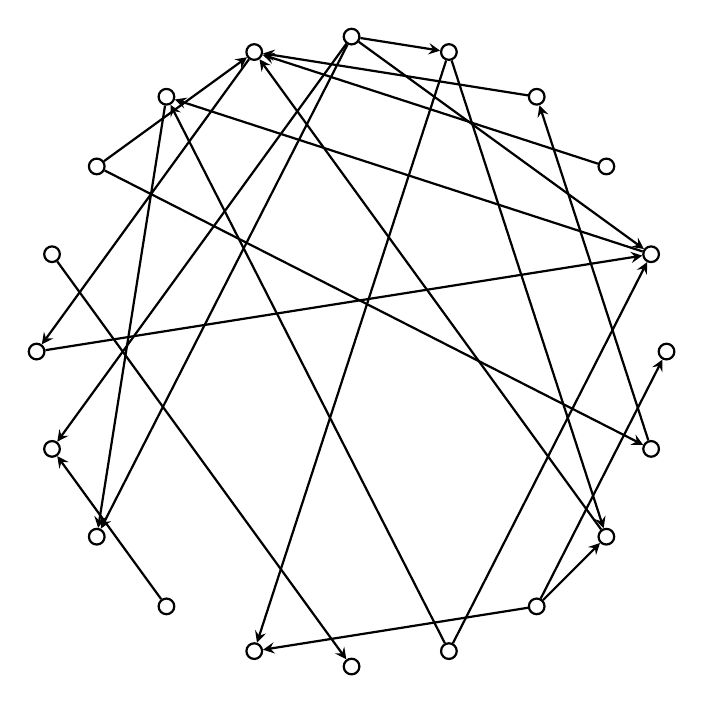
\begin{tikzpicture}
[lineDecorate/.style={->,>=stealth,thick},%
  nodeDecorate/.style={shape=circle,inner sep=2pt,draw,thick},
  scale=4]
%% nodes or vertices
\foreach \nodename/\x/\y in {
  0/1.00000000000000/0.000000000000000,
  1/0.951056516295154/0.309016994374947,
  2/0.809016994374947/0.587785252292473,
  3/0.587785252292473/0.809016994374947,
  4/0.309016994374947/0.951056516295154,
  5/0.000000000000000/1.00000000000000,
  6/-0.309016994374947/0.951056516295154,
  7/-0.587785252292473/0.809016994374947,
  8/-0.809016994374947/0.587785252292473,
  9/-0.951056516295154/0.309016994374947,
  10/-1.00000000000000/0.000000000000000,
  11/-0.951056516295154/-0.309016994374947,
  12/-0.809016994374947/-0.587785252292473,
  13/-0.587785252292473/-0.809016994374947,
  14/-0.309016994374947/-0.951056516295154,
  15/0.000000000000000/-1.00000000000000,
  16/0.309016994374947/-0.951056516295154,
  17/0.587785252292473/-0.809016994374947,
  18/0.809016994374947/-0.587785252292473,
  19/0.951056516295154/-0.309016994374947}
{
  \node (\nodename) at (\x,\y) [nodeDecorate] {};
}
%% edges or lines
\path
\foreach \startnode/\endnode in {
  1/7, 2/6, 3/6, 4/14, 4/18, 5/1, 5/4, 5/11, 5/12, 6/10, 7/12, 8/6,
  8/19, 9/15, 10/1, 13/11, 16/1, 16/7, 17/0, 17/14, 17/18, 18/6, 19/3}
{
  (\startnode) edge[lineDecorate] node {} (\endnode)
};
\end{tikzpicture}
\end{figure}

\end{document}

\caption{A random oriented graph generated using a graph in
  $G(20,\, 0.1)$ and cutoff probability $0.5$.}
\label{fig:random_graphs:random_oriented_graph}
\end{figure}


%%%%%%%%%%%%%%%%%%%%%%%%%%%%%%%%%%%%%%%%%%%%%%%%%%%%%%%%%%%%%%%%%%%%%%%%%%%

\subsubsection{Degree distribution}
\index{degree distribution}

Consider a random graph $G \in \cG(n,p)$ and let $v$ be a vertex of
$G$. With probability $p$, the vertex $v$ is incident with each of the
remaining $n - 1$ vertices in $G$. Then the probability that $v$ has
degree $k$ is given by the binomial\index{distribution!binomial}
distribution
%%
\begin{equation}
\label{eqn:random_graphs:Erdos_Renyi:probability_v_has_degree_k}
\Pr[\deg(v) = k]
=
\binom{n-1}{k} p^k (1 - p)^{n-1-k}
\end{equation}
%%
and the expected degree of $v$ is $\E[\deg(v)] = p(n-1)$. Setting
$z = p(n-1)$, we can
express~\eqref{eqn:random_graphs:Erdos_Renyi:probability_v_has_degree_k}
as
\[
\Pr[\deg(v) = k]
=
\binom{n-1}{k}
\left( \frac{z} {n-1-z} \right)^k
\left( 1 - \frac{z}{n-1} \right)^{n-1}
\]
and thus
\[
\Pr[\deg(v) = k]
\to
\frac{z^k}{k!} \exp(-z)
\]
as $n \to \infty$. In the limit of large $n$, the probability that
vertex $v$ has degree $k$ approaches the
Poisson\index{distribution!Poisson} distribution. That is, as $n$ gets
larger and larger any random graph in $\cG(n,p)$ has a Poisson degree
distribution.


%% One of the first properties of random graphs which makes them so pleasant to work with is the following

%% \begin{theorem}
%%   Let $H$ be any graph, and $0<p<1$. Then
%% $$\lim_{n\to +\infty}P\left[H\text{ is an induced subgraph of }G_{n,p}\right]=1$$
%% \end{theorem}
%% \begin{proof}[Sketch]
%% Instinctively, we would like to find a copy of $H$ in $G_{n,p}$ by iteratively finding an acceptable representant $h(v_i)$ in $G_{n,p}$ of every vertex $v_i$ of $V(H) = \{v_1, \dots, v_k\}$. How could such a strategy work ?
%% \begin{itemize}
%% \item Pick for $v_1$ any vertex $h(v_1)\in G_{n,p}$
%% \item Pick for $v_2$ any vertex $h(v_2)\in G_{n,p}$ such that $h(v_1)h(v_2)\in E(G_{n,p})$ if $v_1v_2\in E(H)$, and such that $h(v_1)h(v_2)\not \in E(G_{n,p})$ otherwise
%% \item \dots
%% \item Assuming you have found, for all $i\leq j\leq k$, a representant $h(v_i)$ for each vertex $v_i$, and such that $H[\{v_1,\dots,v_{j-1}\}]$ is isomorphic to $G_{n,p}[\{h(v_1),\dots,h(v_{j-1})\}]$, try to find a new vertex $h(v_j)$ such that $\forall i<j,h(v_i)h(v_j)\in E(G_{n,p})$ if  and only if $v_iv_j\in E(H)$.

%%   When $n$ is growing large, such a vertex will exist with high probability.
%% \end{itemize}
%% \end{proof}

%% \begin{proof}
%%   Formally, let us write $H_i = H[\{v_1,\dots,v_{j-1}\}]$, and denote
%%   the probability that $H$ is an induced subgraph of $G_{n,p}$ by $P[H
%%     \mapsto_{ind} G_{n,p}]$. We can roughly bound the probability that $H_i$, but not $H_{i+1}$, is an induced subgraph of $G_{n,p}$ the following way :

%%   \begin{itemize}
%%   \item We put a copy of $H_i$ at any of the $\binom n i$ different $i$-subsets of $V(G_{n,p})$.

%%     This can be done, each time, in $i!$ different ways as the vertices $\{v_1, \dots, v_i\}$ can be permuted

%%   \item We compute the probability that no other vertex of $G_{n,p}$ can be used to complete our current copy of $H_i$ into a copy of $H_{i+1}$. The probability that such a vertex is acceptable being
%%     $$p^{d_{H_{i+1}}(v_{i+1})}(1-p)^{i-d_{H_{i+1}}(v_{i+1})}\geq min(p, 1-p)^i$$
%%     the property that none of the $n-i$ vertices left is acceptable is at most
%%     $$\left({ 1- min(p, 1-p)^i } \right)^{(n-i)}$$
%%   \end{itemize}

%%   As $0<p<1$, we can write $0<\epsilon = min(p, 1-p)$ and thus, the probability that $H_i$, but not $H_{i+1}$, is a induced subgraph of $G_{n,p}$ is at most $$i!\binom n i (1-\epsilon^i)^{n-i}\leq i! n^i (1-\epsilon^i)^{n-i} = o(1/n)$$
%% Which is asymptotically equal to 0 as $n$ grows.

%% Thus

%% \begin{align*}
%%   P[H \mapsto_{ind} G_{n,p}]&=1 - P[H_2 \mapsto_{ind} G_{n,p}, H_3\not \mapsto_{ind} G_{n,p}]\\
%%   &-P[H_3 \mapsto_{ind} G_{n,p}, H_4\not \mapsto_{ind} G_{n,p}]\\
%%   &\dots\\
%%   &-P[H_{k-1} \mapsto_{ind} G_{n,p}, H_k\not \mapsto_{ind} G_{n,p}]\\
%%   P[H \mapsto_{ind} G_{n,p}]&\geq 1-\sum_{i\leq k}i!n^i(1-\epsilon^i)^{n-i}\\
%%   &\geq 1-k\times o(1/n)\\
%% \end{align*}

%% Which proves the result.

%% \end{proof}

%% This proof also gives us a simple algorithm to find a copy of a graph $H$ into a random graph $G_{n,p}$. While obviously such an algorithm will not always find the copy of $H$ if it exists, the probability of a successful run will tend toward $1$ as proved immediately above.

%% \begin{lstlisting}
%% def find_induced(H, G):

%%     # f is the function from V(H) to V(G) we
%%     # are attempting to define
%%     f = {}

%%     # leftovers is the set of vertices of G which have not yet
%%     # been used by f
%%     G_leftovers = G.vertices()

%%     # Set of vertices for which no representant has been found yet
%%     H_leftovers = H.vertices()

%%     # While the function is not complete
%%     while H_leftovers:

%%         # We look for the next vertex of H
%%         v = H_leftovers.pop(0)

%%         # ... and look for its possible image
%%         candidates = [u for u in G_leftovers if
%%           all([ H.has_edge(h,v) == G.has_edge(f_h,u)
%%             for h,f_h in f.iteritems()])]

%%         if not candidates:
%%             raise ValueError("No copy of H has been found in G")

%%         # We pick the first of them
%%         f[v] = candidates[0]
%%         G_leftovers.remove(f[v])

%%     return f
%% \end{lstlisting}


%%%%%%%%%%%%%%%%%%%%%%%%%%%%%%%%%%%%%%%%%%%%%%%%%%%%%%%%%%%%%%%%%%%%%%%%%%%

\section{Small-world networks}
\label{sec:random_graphs:small_world_networks}

Many real-world networks exhibit the
\emph{small-world effect}\index{small-world!effect}: that most pairs
of distinct vertices in the network are connected by relatively short
path lengths. The small-world effect was empirically
demonstrated~\cite{Milgram1967} in a famous~1960s experiment by
Stanley Milgram\index{Milgram, Stanley}, who distributed a number
of letters to a random selection of people. Recipients were instructed
to deliver the letters to the addressees on the condition that letters
must be passed to people whom the recipients knew on a first-name
basis. Milgram found that on average six steps were required for a
letter to reach its target recipient, a number now immortalized in the
phrase\index{six degrees of separation} ``six degrees of
separation''~\cite{Guare1990}.
Figure~\ref{fig:random_graphs:Milgram_small_world_experiment_results}
plots results of an experimental study of the small-world problem as
reported in~\cite{TraversMilgram1969}. The small-world effect has been
studied and verified for many real-world networks including
%%
\begin{itemize}
\item social\index{network!social}: collaboration network of actors in
  feature films~\cite{AmaralEtAl2000,WattsStrogatz1998}, scientific
  publication
  authorship~\cite{CastroGrossman1999,GrossmanIon1995,Newman2001a,Newman2001b};

\item information\index{network!information}: citation
  network~\cite{Redner1998}, Roget's\index{Roget's Thesaurus}
  Thesaurus~\cite{Knuth1993}, word
  co-occurrence~\cite{DorogovtsevMendes2001,FerrerSole2001};

\item technological\index{network!technological}:
  internet~\cite{ChenEtAl2002,FaloutsosEtAl1999}, power
  grid~\cite{WattsStrogatz1998}, train routes~\cite{SenEtAl2003},
  software~\cite{Newman2003a,ValverdeEtAl2002};

\item biological\index{network!biological}: metabolic
  network~\cite{JeongEtAl2000}, protein
  interactions~\cite{JeongEtAl2001}, food
  web~\cite{HuxhamEtAl1996,Martinez1991}, neural
  network~\cite{WattsStrogatz1998,WhiteEtAl1986}.
\end{itemize}

\begin{figure}[!htbp]
\centering
\index{frequency distribution}
\index{small-world!experimental results}
%%%%%%%%%%%%%%%%%%%%%%%%%%%%%%%%%%%%%%%%%%%%%%%%%%%%%%%%%%%%%%%%%%%%%%%%%%%
%% This file is part of the book
%%
%% Algorithmic Graph Theory
%% http://code.google.com/p/graph-theory-algorithms-book/
%%
%% Copyright (C) 2009, 2010, 2011 Minh Van Nguyen <nguyenminh2@gmail.com>
%%
%% See the file COPYING for copying conditions.
%%%%%%%%%%%%%%%%%%%%%%%%%%%%%%%%%%%%%%%%%%%%%%%%%%%%%%%%%%%%%%%%%%%%%%%%%%%

\documentclass{article}

\usepackage{amsmath}
\usepackage{pgfplots}
\usetikzlibrary{external}
\tikzexternalize{Milgram-small-world-experiment-results}

\begin{document}

\begin{figure}
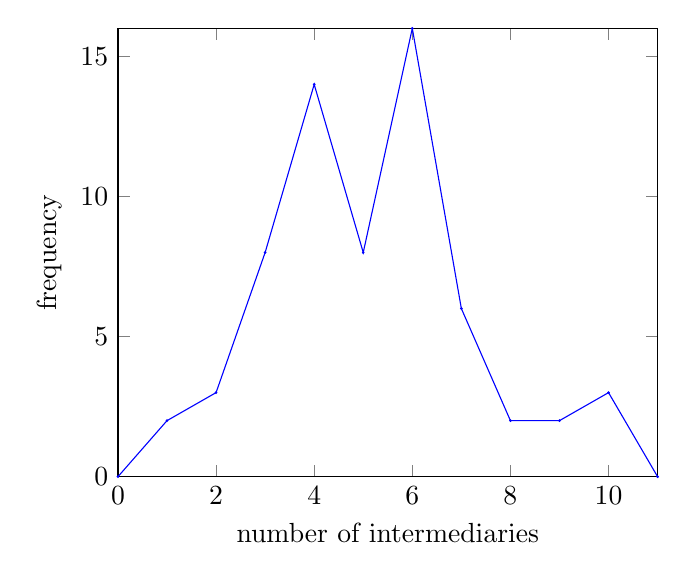
\begin{tikzpicture}
[every mark/.append style={scale=0.5}]
\begin{axis}[%
  enlargelimits=false,%
  xlabel=\text{number of intermediaries},%
  ylabel=\text{frequency}%
]
\addplot+[sharp plot] coordinates
{(0,0)  (1,2)  (2,3) (3,8) (4,14)%
 (5,8)  (6,16) (7,6) (8,2) (9,2)%
 (10,3) (11,0)
};
\end{axis}
\end{tikzpicture}
\end{figure}

\end{document}

\caption{Frequency distribution of the number of intermediaries
  required for letters to reach their intended addressees. The
  distribution has a mean of $5.3$, interpreted as the average number
  of intermediaries required for a letter to reach its intended
  destination. The plot is derived from data reported in Travers and
  Milgram~\cite{TraversMilgram1969}.}
\label{fig:random_graphs:Milgram_small_world_experiment_results}
\end{figure}

Watts\index{Watts, Duncan J.} and\index{Strogatz, Steven H.}
Strogatz~\cite{Watts1999a,Watts1999b,WattsStrogatz1998}
proposed a network model that produces graphs exhibiting the
small-world effect. Let $n$ and $k$ be positive integers such that
$n \gg k \gg \ln n \gg 1$~(in particular, $0 < k < n/2$), $k$ being
even, and consider a probability $0 < p < 1$. Starting from an
undirected $k$-circulant\index{regular graph!$k$-circulant} graph
$G = (V,E)$ on $n$ vertices, the
Watts-Strogatz\index{Watts-Strogatz model} model proceeds to rewire
each edge with probability $p$. The rewiring procedure works as
follows. Let $V$ be uniformly distributed. For each $v \in V$, let
$e \in E$ be an edge having $v$ as an endpoint. Choose another
$u \in V$ different from $v$. With probability $p$, delete the edge
$e$ and add the edge $vu$. The rewiring must produce a
simple\index{simple graph} graph with the same order and size as
$G$. As $p \to 1$, the graph $G$ goes from $k$-circulant to exhibiting
properties of $\cG(n,p)$\index{random graph!binomial}. Small-world
networks are intermediate between $k$-circulant and binomial random
graphs~(see
Figure~\ref{fig:random_graphs:k_circulant_small_world_random}). The
Watts-Strogatz model is said to provide a procedure for interpolating
between the latter two types of graphs.

\begin{figure}[!htbp]
\centering
%%%%%%%%%%%%%%%%%%%%%%%%%%%%%%%%%%%%%%%%%%%%%%%%%%%%%%%%%%%%%%%%%%%%%%%%%%%
%% This file is part of the book
%%
%% Algorithmic Graph Theory
%% http://code.google.com/p/graph-theory-algorithms-book/
%%
%% Copyright (C) 2009, 2010, 2011 Minh Van Nguyen <nguyenminh2@gmail.com>
%%
%% See the file COPYING for copying conditions.
%%%%%%%%%%%%%%%%%%%%%%%%%%%%%%%%%%%%%%%%%%%%%%%%%%%%%%%%%%%%%%%%%%%%%%%%%%%

\subfigure[$p = 0$, $k$-circulant]{
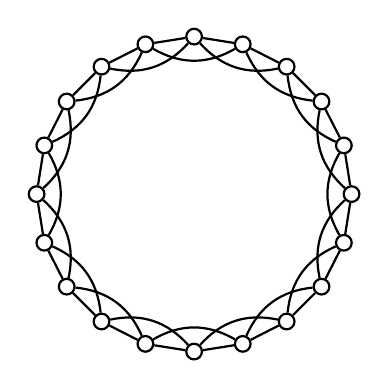
\begin{tikzpicture}
[lineDecorate/.style={-,thick},%
  nodeDecorate/.style={shape=circle,inner sep=2pt,draw,thick},
  scale=2]
%% nodes or vertices
\foreach \nodename/\x/\y in {
  0/1.00000000000000/0.000000000000000,
  1/0.951056516295154/0.309016994374947,
  2/0.809016994374947/0.587785252292473,
  3/0.587785252292473/0.809016994374947,
  4/0.309016994374947/0.951056516295154,
  5/0.000000000000000/1.00000000000000,
  6/-0.309016994374947/0.951056516295154,
  7/-0.587785252292473/0.809016994374947,
  8/-0.809016994374947/0.587785252292473,
  9/-0.951056516295154/0.309016994374947,
  10/-1.00000000000000/0.000000000000000,
  11/-0.951056516295154/-0.309016994374947,
  12/-0.809016994374947/-0.587785252292473,
  13/-0.587785252292473/-0.809016994374947,
  14/-0.309016994374947/-0.951056516295154,
  15/0.000000000000000/-1.00000000000000,
  16/0.309016994374947/-0.951056516295154,
  17/0.587785252292473/-0.809016994374947,
  18/0.809016994374947/-0.587785252292473,
  19/0.951056516295154/-0.309016994374947}
{
  \node (\nodename) at (\x,\y) [nodeDecorate] {};
}
%% edges or lines
\path
\foreach \startnode/\endnode in {
  0/1, 0/19, 1/2, 2/3, 3/4, 4/5, 5/6, 6/7, 7/8, 8/9, 9/10, 10/11,
  11/12, 12/13, 13/14, 14/15, 15/16, 16/17, 17/18, 18/19}
{
  (\startnode) edge[lineDecorate] node {} (\endnode)
}
\foreach \startnode/\endnode in {
  0/2, 1/3, 2/4, 3/5, 4/6, 5/7, 6/8, 7/9, 8/10, 9/11, 10/12, 11/13,
  12/14, 13/15, 14/16, 15/17, 16/18, 17/19, 18/0, 19/1}
{
  (\startnode) edge[lineDecorate,bend left] node {} (\endnode)
};
\end{tikzpicture}
}
%%
%%
\qquad
\subfigure[$p = 0.3$, small-world]{
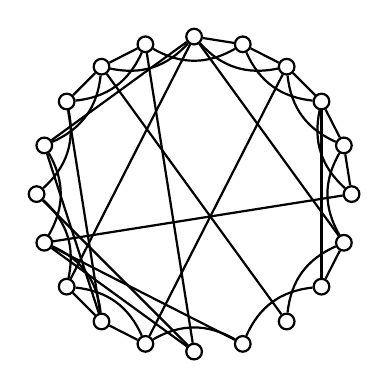
\begin{tikzpicture}
[lineDecorate/.style={-,thick},%
  nodeDecorate/.style={shape=circle,inner sep=2pt,draw,thick},
  scale=2]
%% nodes or vertices
\foreach \nodename/\x/\y in {
  0/1.00000000000000/0.000000000000000,
  1/0.951056516295154/0.309016994374947,
  2/0.809016994374947/0.587785252292473,
  3/0.587785252292473/0.809016994374947,
  4/0.309016994374947/0.951056516295154,
  5/0.000000000000000/1.00000000000000,
  6/-0.309016994374947/0.951056516295154,
  7/-0.587785252292473/0.809016994374947,
  8/-0.809016994374947/0.587785252292473,
  9/-0.951056516295154/0.309016994374947,
  10/-1.00000000000000/0.000000000000000,
  11/-0.951056516295154/-0.309016994374947,
  12/-0.809016994374947/-0.587785252292473,
  13/-0.587785252292473/-0.809016994374947,
  14/-0.309016994374947/-0.951056516295154,
  15/0.000000000000000/-1.00000000000000,
  16/0.309016994374947/-0.951056516295154,
  17/0.587785252292473/-0.809016994374947,
  18/0.809016994374947/-0.587785252292473,
  19/0.951056516295154/-0.309016994374947}
{
  \node (\nodename) at (\x,\y) [nodeDecorate] {};
}
%% edges or lines
\path
\foreach \startnode/\endnode in {
  0/1, 0/11, 1/2, 2/3, 2/18, 3/4, 3/14, 4/5, 5/9, 5/12, 5/19,
  6/7, 6/15, 7/8, 7/17, 8/13, 9/13, 10/15, 11/15, 11/16, 12/13, 13/14,
  18/19}
{
  (\startnode) edge[lineDecorate] node {} (\endnode)
}
\foreach \startnode/\endnode in {
  0/2, 1/3, 2/4, 3/5, 4/6, 5/7, 6/8, 7/9, 8/10, 9/11, 10/12, 11/13,
  12/14, 14/16, 16/18, 17/19, 19/1}
{
  (\startnode) edge[lineDecorate,bend left] node {} (\endnode)
};
\end{tikzpicture}
}
%%
%%
\qquad
\subfigure[$p = 1$, random]{
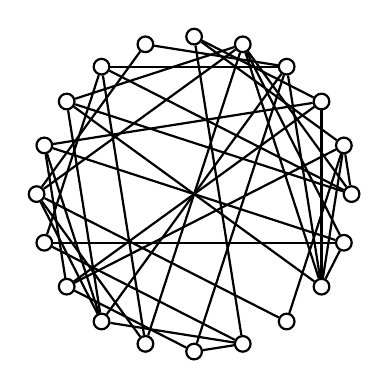
\begin{tikzpicture}
[lineDecorate/.style={-,thick},%
  nodeDecorate/.style={shape=circle,inner sep=2pt,draw,thick},
  scale=2]
%% nodes or vertices
\foreach \nodename/\x/\y in {
  0/1.00000000000000/0.000000000000000,
  1/0.951056516295154/0.309016994374947,
  2/0.809016994374947/0.587785252292473,
  3/0.587785252292473/0.809016994374947,
  4/0.309016994374947/0.951056516295154,
  5/0.000000000000000/1.00000000000000,
  6/-0.309016994374947/0.951056516295154,
  7/-0.587785252292473/0.809016994374947,
  8/-0.809016994374947/0.587785252292473,
  9/-0.951056516295154/0.309016994374947,
  10/-1.00000000000000/0.000000000000000,
  11/-0.951056516295154/-0.309016994374947,
  12/-0.809016994374947/-0.587785252292473,
  13/-0.587785252292473/-0.809016994374947,
  14/-0.309016994374947/-0.951056516295154,
  15/0.000000000000000/-1.00000000000000,
  16/0.309016994374947/-0.951056516295154,
  17/0.587785252292473/-0.809016994374947,
  18/0.809016994374947/-0.587785252292473,
  19/0.951056516295154/-0.309016994374947}
{
  \node (\nodename) at (\x,\y) [nodeDecorate] {};
}
%% edges or lines
\path
\foreach \startnode/\endnode in {
  0/1, 0/4, 0/7, 0/8, 1/5, 1/12, 1/17, 1/18, 2/5, 2/9, 2/12, 2/18, 3/6,
  3/7, 3/13, 3/15, 3/18, 4/8, 4/10, 4/14, 4/18, 4/19, 5/16, 6/10, 7/11,
  7/14, 8/13, 8/18, 9/12, 9/13, 9/19, 10/13, 10/14, 10/17, 11/16, 11/19,
  12/15, 13/16, 15/16, 18/19}
{
  (\startnode) edge[lineDecorate] node {} (\endnode)
};
\end{tikzpicture}
}

\caption{With increasing randomness, $k$-circulant graphs evolve to
  exhibit properties of random graphs in $\cG(n,p)$. Small-world
  networks are intermediate between $k$-circulant graphs and random
  graphs in $\cG(n,p)$.}
\label{fig:random_graphs:k_circulant_small_world_random}
\end{figure}

The last paragraph contains an algorithm for rewiring edges of a
graph. While the algorithm is simple, in practice it potentially skips
over a number of vertices to be considered for rewiring. If
$G = (V,E)$ is a $k$-circulant graph on $n$ vertices and $p$ is the
rewiring probability, the candidate vertices to be rewired follow a
geometric distribution with parameter $p$. This geometric trick,
essentially the same speed-up technique used by the Batagelj-Brandes
Algorithm~\ref{alg:random_graphs:linear_generate_random_sparse_Gnp},
can be used to speed up the rewiring algorithm. To elaborate, suppose
$G$ has vertex set $V = \{0, 1, \dots, n-1\}$. If $r$ is chosen
uniformly at random from the interval $(0,1)$, the index of the vertex
to be rewired can be obtained from
\[
1 + \left\lfloor \frac{\ln(1 - r)} {\ln(1 - p)} \right\rfloor.
\]
The above geometric method is incorporated into
Algorithm~\ref{alg:random_graphs:generate_Watts_Strogatz_graph} to
generate a Watts-Strogatz network in worst-case runtime
$O(nk + m)$, where $n$ and $k$ are as per the input of the algorithm
and $m$ is the size of the $k$-circulant graph on $n$ vertices. Note
that lines~\ref{alg:Watts_Strogatz:even_index}
to~\ref{alg:Watts_Strogatz:choose_vertex_odd_index} are where we avoid
self-loops and multiple edges.

\begin{algorithm}[!htbp]
\index{algorithm!random}
\index{complete graph}
\index{list!contiguous edge}
\index{regular graph!$k$-circulant}
\index{small-world!algorithm}
\index{small-world!network}
\index{Watts-Strogatz model}
%%%%%%%%%%%%%%%%%%%%%%%%%%%%%%%%%%%%%%%%%%%%%%%%%%%%%%%%%%%%%%%%%%%%%%%%%%%
%% This file is part of the book
%%
%% Algorithmic Graph Theory
%% http://code.google.com/p/graph-theory-algorithms-book/
%%
%% Copyright (C) 2009, 2010, 2011 Minh Van Nguyen <nguyenminh2@gmail.com>
%%
%% See the file COPYING for copying conditions.
%%%%%%%%%%%%%%%%%%%%%%%%%%%%%%%%%%%%%%%%%%%%%%%%%%%%%%%%%%%%%%%%%%%%%%%%%%%

\DontPrintSemicolon
\SetAlgoNoLine
%%
%% data section
\SetKwInOut{Input}{Input}
\SetKwInOut{Output}{Output}
%%
%% input/output
\Input{Positive integer $n$ denoting the number of vertices. Positive
  even integer $k$ for the degree of each vertex, where
  $n \gg k \gg \ln n \gg 1$. In particular, $k$ should satisfy
  $0 < k < n/2$. Rewiring probability $0 < p \leq 1$.}
\Output{A Watts-Strogatz network on $n$ vertices.}
\BlankLine
%%
%% algorithm body
$M \assign nk$~\tcc*[f]{sum of all vertex degrees = twice number of edges}\;
$r \assign$ draw uniformly at random from $[0,1)$\;
$v \assign 1 + \lfloor \log(1 - r) / \log(1 - p) \rfloor$\;
$E \assign$ contiguous edge list of $k$-circulant graph on $n$ vertices\;
\While{$v \leq M$}{
  $u \assign$ draw uniformly at random from $[0, 1, \dots, n-1]$\;
  $E[v-1] \assign u$\;
  $r \assign$ draw uniformly at random from $[0,1)$\;
  $v \assign v + 1 + \lfloor \log(1 - r) / \log(1 - p) \rfloor$\;
}
$G \assign \overline{K_n}$\;
$\ell \assign |E|$\;
add edge $v_i v_{i+1}$ to $G$ for even $0 \leq i \leq \ell - 2$\;
\Return $G$\;

\caption{Watts-Strogatz network model.}
\label{alg:random_graphs:generate_Watts_Strogatz_graph}
\end{algorithm}


%%%%%%%%%%%%%%%%%%%%%%%%%%%%%%%%%%%%%%%%%%%%%%%%%%%%%%%%%%%%%%%%%%%%%%%%%%%

\subsubsection{Characteristic path length}

Watts and Strogatz~\cite{WattsStrogatz1998} analyzed the structure of
networks generated by
Algorithm~\ref{alg:random_graphs:generate_Watts_Strogatz_graph} via
two quantities: the
\emph{characteristic path length}\index{small-world!characteristic path length}
$\ell$ and the
\emph{clustering coefficient}\index{small-world!clustering coefficient}
$C$. The characteristic path length quantifies the average distance
between any distinct pair of vertices in a Watts-Strogatz network. The
quantity $\ell(G)$ is thus said to be a global property of $G$. Watts
and Strogatz characterized as \emph{small-world}\index{small-world}
those networks that exhibit high clustering coefficients and low
characteristic path lengths.

Let $G = (V,E)$ be a Watts-Strogatz network as generated by
Algorithm~\ref{alg:random_graphs:generate_Watts_Strogatz_graph}, where
the vertex set is $V = \{0, 1, \dots, n-1\}$. For each pair of
vertices $i,j \in V$, let $d_{ij}$ be the distance from $i$ to $j$. If
there is no path from $i$ to $j$ or $i = j$, set $d_{ij} = 0$. Thus
\[
d_{ij}
=
\begin{cases}
0, & \text{if there is no path from $i$ to $j$}, \\[4pt]
0, & \text{if $i = j$}, \\[4pt]
k, & \text{where $k$ is the length of a shortest path from $i$ to $j$}.
\end{cases}
\]
Since $G$ is undirected, we have $d_{ij} = d_{ji}$. Consequently when
computing the distance between each distinct pair of vertices, we
should avoid double counting by computing $d_{ij}$ for $i < j$. Then
the characteristic path length of $G$ is defined by
%%
\begin{equation}
\label{eqn:random_graphs:define_characteristic_path_length}
\begin{aligned}
\ell(G)
&=
\frac{1}{n(n-1)/2} \cdot \frac{1}{2} \sum_{i \neq j} d_{ij} \\[4pt]
&=
\frac{1}{n(n-1)} \sum_{i \neq j} d_{ij}
\end{aligned}
\end{equation}
%%
which is averaged over all possible pairs of distinct vertices,
i.e. the number of edges in the complete\index{complete graph} graph
$K_n$.

It is inefficient to compute the characteristic path length via
equation~\eqref{eqn:random_graphs:define_characteristic_path_length}
because we would effectively sum $n(n - 1)$ distance values. As $G$ is
undirected, note that
\[
\frac{1}{2} \sum_{i \neq j} d_{ij}
=
\sum_{i < j} d_{ij}
=
\sum_{i > j} d_{ij}.
\]
The latter equation holds for the following reason. Let $D = [d_{ij}]$
be a matrix of distances for $G$, where $i$ is the row index, $j$ is
the column index, and $d_{ij}$ is the distance from $i$ to $j$. The
required sum of distances can be obtained by summing all entries
above~(or below) the main diagonal of $D$. Therefore the
characteristic path length can be expressed as
%%
\begin{align*}
\ell(G)
&=
\frac{2}{n(n-1)} \sum_{i < j} d_{ij} \\[4pt]
&=
\frac{2}{n(n-1)} \sum_{i > j} d_{ij}
\end{align*}
%%
which requires summing $\frac{n(n-1)}{2}$ distance values.

Let $G = (V,E)$ be a Watts-Strogatz network with $n = |V|$. Set
$k' = k/2$, where $k$ is as per
Algorithm~\ref{alg:random_graphs:generate_Watts_Strogatz_graph}. As
the rewiring probability $p \to 0$, the average path length tends to
\[
\ell
\to
\frac{n}{4k'}
=
\frac{n}{2k}.
\]
In the special case $p = 0$, we have
\[
\ell
=
\frac{n (n + k - 2)} {2k (n - 1)}.
\]
However as $p \to 1$, we have $\ell \to \frac{\ln n} {\ln k}$.


%%%%%%%%%%%%%%%%%%%%%%%%%%%%%%%%%%%%%%%%%%%%%%%%%%%%%%%%%%%%%%%%%%%%%%%%%%%

\subsubsection{Clustering coefficient}

The \emph{clustering coefficient}\index{small-world!clustering coefficient} of a
simple graph $G$ quantifies the ``cliquishness'' of vertices in
$G = (V,E)$. This quantity is thus said to be a local property of
$G$. Watts and Strogatz~\cite{WattsStrogatz1998} defined the
clustering coefficient as follows. Suppose $n = |V| > 0$ and let $n_i$
count the number of neighbors of vertex $i \in V$, a quantity that is
equivalent to the degree of $i$, i.e. $\deg(i) = n_i$. The complete
graph $K_{n_i}$ on the $n_i$ neighbors of $i$ has $n_i(n_i - 1) / 2$
edges. The \emph{neighbor graph}\index{neighbor graph}\index{$\cN_i$}
$\cN_i$ of $i$ is a subgraph of $G$, consisting of all
vertices~($\neq i$) that are adjacent to $i$ and preserving the
adjacency relation among those vertices as found in the supergraph
$G$. For example, given the graph in
Figure~\ref{fig:neighbor_graph:original_graph} the neighbor graph of
vertex $10$ is shown in
Figure~\ref{fig:neighbor_graph:neighbor_graph}. The local clustering
coefficient $C_i$ of $i$ is the ratio
\[
C_i
=
\frac{N_i} {n_i (n_i - 1) / 2}
\]
where $N_i$ counts the number of edges in $\cN_i$. In case $i$ has
degree $\deg(i) < 2$, we set the local clustering coefficient of $i$
to be zero. Then the clustering
coefficient\index{small-world!clustering coefficient} of $G$ is defined by
\[
C(G)
=
\frac{1}{n} \sum_{i \in V} C_i
=
\frac{1}{n} \sum_{i \in V} \frac{N_i} {n_i (n_i - 1) / 2}.
\]

\begin{figure}[!htbp]
\centering
\index{neighbor graph}
%%%%%%%%%%%%%%%%%%%%%%%%%%%%%%%%%%%%%%%%%%%%%%%%%%%%%%%%%%%%%%%%%%%%%%%%%%%
%% This file is part of the book
%%
%% Algorithmic Graph Theory
%% http://code.google.com/p/graph-theory-algorithms-book/
%%
%% Copyright (C) 2009--2011 Minh Van Nguyen <nguyenminh2@gmail.com>
%%
%% See the file COPYING for copying conditions.
%%%%%%%%%%%%%%%%%%%%%%%%%%%%%%%%%%%%%%%%%%%%%%%%%%%%%%%%%%%%%%%%%%%%%%%%%%%

\documentclass{article}

\usepackage{subfigure}
\usepackage{tikz}
\usetikzlibrary{external}
\tikzexternalize{neighbor-graph}
\newcommand{\cN}{\mathcal{N}}

\begin{document}

\begin{figure}
\subfigure[Graph on $11$ vertices.]{
\label{fig:neighbor_graph:original_graph}
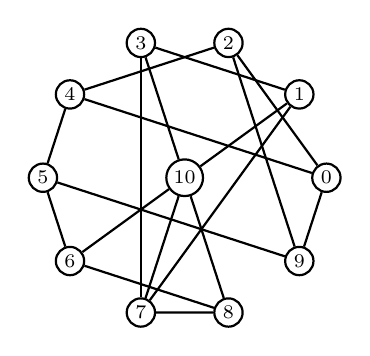
\begin{tikzpicture}
[lineDecorate/.style={-,thick},%
  nodeDecorate/.style={shape=circle,inner sep=1.5pt,draw,thick},
  scale=1.8]
\scriptsize
%% nodes or vertices
\foreach \nodename/\x/\y in {
  0/1.00000000000000/0.000000000000000,
  1/0.809016994374947/0.587785252292473,
  2/0.309016994374947/0.951056516295154,
  3/-0.309016994374947/0.951056516295154,
  4/-0.809016994374947/0.587785252292473,
  5/-1.00000000000000/0.000000000000000,
  6/-0.809016994374947/-0.587785252292473,
  7/-0.309016994374947/-0.951056516295154,
  8/0.309016994374947/-0.951056516295154,
  9/0.809016994374947/-0.587785252292473,
  10/0/0}
{
  \node (\nodename) at (\x,\y) [nodeDecorate] {$\nodename$};
}
%% edges or lines
\path
\foreach \startnode/\endnode in {
  0/2, 0/4, 0/9, 1/3, 1/7, 2/4, 2/9, 3/7, 4/5, 5/6, 5/9, 6/8, 7/8,
  10/1, 10/3, 10/6, 10/7, 10/8}
{
  (\startnode) edge[lineDecorate] node {} (\endnode)
};
\end{tikzpicture}
}
%%
%%
\qquad
\subfigure[$\cN_{10}$]{
\label{fig:neighbor_graph:neighbor_graph}
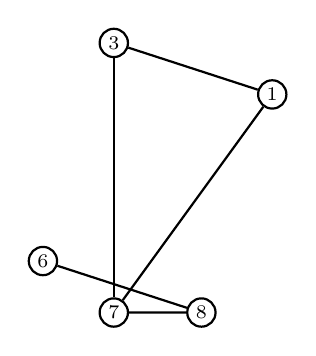
\begin{tikzpicture}
[lineDecorate/.style={-,thick},%
  nodeDecorate/.style={shape=circle,inner sep=1.5pt,draw,thick},
  scale=1.8]
\scriptsize
%% nodes or vertices
\foreach \nodename/\x/\y in {
  1/0.809016994374947/0.587785252292473,
  3/-0.309016994374947/0.951056516295154,
  6/-0.809016994374947/-0.587785252292473,
  7/-0.309016994374947/-0.951056516295154,
  8/0.309016994374947/-0.951056516295154}
{
  \node (\nodename) at (\x,\y) [nodeDecorate] {$\nodename$};
}
%% edges or lines
\path
\foreach \startnode/\endnode in {1/3, 1/7, 3/7, 6/8, 7/8}
{
  (\startnode) edge[lineDecorate] node {} (\endnode)
};
\end{tikzpicture}
}
\end{figure}

\end{document}

\caption{The neighbor graph of a vertex.}
\label{fig:random_graphs:neighbor_graph}
\end{figure}

Consider the case where we have a $k$-circulant graph
$G = (V,E)$ on $n$ vertices and a rewiring probability $p = 0$. That
is, we do not rewire any edge of $G$. Each vertex of $G$ has degree
$k$. Let  $k' = k/2$. Then the $k$ neighbors of each vertex in $G$ has
$3k' (k' - 1) / 2$ edges between them, i.e. each neighbor graph
$\cN_i$ has size $3k' (k' - 1) / 2$. Then the clustering coefficient
of $G$ is
\[
\frac{3(k' - 1)} {2(2k' - 1)}.
\]
When the rewiring probability is $p > 0$, Barrat and
Weigt~\cite{BarratWeigt2000} showed that the clustering coefficient of
any graph $G'$ in the Watts-Strogatz network model~(see
Algorithm~\ref{alg:random_graphs:generate_Watts_Strogatz_graph}) can
be approximated by
\[
C(G')
\approx
\frac{3(k' - 1)} {2(2k' - 1)} (1 - p)^3.
\]


%%%%%%%%%%%%%%%%%%%%%%%%%%%%%%%%%%%%%%%%%%%%%%%%%%%%%%%%%%%%%%%%%%%%%%%%%%%

\subsubsection{Degree distribution}

For a Watts-Strogatz network without rewiring, each vertex has the
same degree $k$. It easily follows that for each vertex $v$, we have
the degree distribution
\[
\Pr[\deg(v) = i]
=
\begin{cases}
1, & \text{if $i = k$}, \\[4pt]
0, & \text{otherwise}.
\end{cases}
\]

A rewiring probability $p > 0$ introduces disorder in the network and
broadens the degree distribution, while the expected degree is $k$. A
$k$-circulant graph on $n$ vertices has $nk / 2$ edges. With the
rewiring probability $p > 0$, a total of $pnk / 2$ edges would be
rewired. However note that only one endpoint of an edge is rewired,
thus after the rewiring process the degree of any vertex $v$ is
$\deg(v) \geq k/2$. Therefore with $ k > 2$, a Watts-Strogatz network
has no isolated vertices.

For $p > 0$, Barrat and Weigt~\cite{BarratWeigt2000} showed that the
degree of a vertex $v$ can be written as $\deg(v) = k/2 + n_i$ with
$n_i \geq 0$, where $n_i$ can be divided into two parts $\alpha$ and
$\beta$ as follows. First $\alpha \leq k/2$ edges are left intact
after the rewiring process, the probability of this occurring is
$1 - p$ for each edge. Second $\beta = n_i - \alpha$ edges have been
rewired towards $i$, each with probability $1/n$. The probability
distribution of $\alpha$ is
\[
P_1(\alpha)
=
\binom{k/2}{\alpha} (1 - p)^\alpha p^{k/2 - \alpha}
\]
and the probability distribution of $\beta$ is
\[
P_2(\beta)
=
\binom{pnk/2}{\beta} \left( \frac{1}{n} \right)^\beta
\left( 1 - \frac{1}{n} \right)^{pnk/2 - \beta}
\]
where
\[
P_2(\beta)
\to
\frac{(pk/2)^\beta}{\beta!} \exp(-pk/2)
\]
for large $n$. Combine the above two factors to obtain the degree
distribution
\[
\Pr[\deg(v) = \kappa]
=
\sum_{i=0}^{\min\{\kappa - k/2,\, k/2\}}
\binom{k/2}{i} (1 - p)^i p^{k/2 - i}
\frac{(pk/2)^{\kappa - k/2 - i}} {(\kappa - k/2 - i)!}
\exp(-pk/2)
\]
for $\kappa \geq k/2$.


%%%%%%%%%%%%%%%%%%%%%%%%%%%%%%%%%%%%%%%%%%%%%%%%%%%%%%%%%%%%%%%%%%%%%%%%%%%

\section{Scale-free networks}

%% The power-law degree distribution model of Barab{\'a}si and
%% Albert~\cite{BarabasiAlbert1999}. See also Bollobas and
%% Riordan~\cite{BollobasRiordan2004},
%% Bollobas~et~al.~\cite{BollobasEtAl2001},
%% Dangalchev~\cite{Dangalchev2004},
%% Newman~\cite{Newman2003b,Newman2005}, Albert and
%% Barab{\'a}si~\cite{AlbertBarabasi2002}.

The networks covered so far---Gilbert $\cG(n,p)$ model,
Erd\H{o}s-R\'enyi $\cG(n,N)$ model, Watts-Strogatz small-world
model---are static. Once a network is generated from any of these
models, the corresponding model does not specify any means for the
network to evolve over time. Barab\'asi and
Albert~\cite{BarabasiAlbert1999} proposed a network model based on two
ingredients:
%%
\begin{enumerate}
\item Growth: at each time step, a new vertex is added to the network
  and connected to a pre-determined number of existing vertices.

\item Preferential attachment\index{preferential attachment}: the
  newly added vertex is connected to an existing vertex in proportion
  to the latter's existing degree.
\end{enumerate}
%%
Preferential attachment\index{preferential attachment} also goes by
the colloquial name of the
``rich-get-richer''\index{rich-get-richer effect} effect due to the
work of Herbert\index{Simon, Herbert} Simon~\cite{Simon1955}. In
sociology, preferential attachment is known as the
\emph{Matthew effect}\index{Matthew effect} due to the following verse
from the Book of Matthew, chapter~25 verse~29, in the Bible: ``For to
every one that hath shall be given but from him that hath not, that
also which he seemeth to have shall be taken away.'' Barab\'asi and
Albert observed that many real-world networks exhibit statistical
properties of their proposed model. One particulary significant
property is that of power-law scaling, hence the
Barab\'asi-Albert\index{Barab\'asi-Albert model} model is also called
a model of scale-free networks. Note that it is only the degree
distributions of scale-free networks that are scale-free. In their
empirical study of the World Wide\index{World Wide Web} Web~(WWW) and
other real-world networks, Barab\'asi and Albert noted that the
probability that a web page increases in popularity is directly
proportional to the page's current popularity. Thinking of a web page
as a vertex and the degree of a page as the number of other pages that
the current page links to, the degree distribution of the WWW follows
a power law function. Power-law scaling has been confirmed for many
real-world
networks:
%%
\begin{itemize}
\item actor collaboration network~\cite{BarabasiAlbert1999}

\item citation~\cite{Price1965,Redner1998,Seglen1992} and
  coauthorship networks~\cite{Newman2001b}

\item human sexual contacts network~\cite{JonesHandcock2003,LiljerosEtAl2001}

\item the\index{Internet}
  Internet~\cite{ChenEtAl2002,FaloutsosEtAl1999,VazquezEtAl2002} and
  the WWW~\cite{AlbertEtAl1999,BarabasiEtAl2000,BroderEtAl2000}

\item metabolic\index{metabolic network}
  networks~\cite{JeongEtAl2001,JeongEtAl2000}

\item telephone call graphs~\cite{AielloEtAl2000,AielloEtAl2002}
\end{itemize}

Figure~\ref{fig:random_graphs:real_world_scale_free_networks}
illustrates the degree distributions of various real-world networks,
plotted on log-log scales. In all of these degree distributions,
self-loops are not taken in account. The actor collaboration
network~\cite{BarabasiAlbert1999}, whose degree distribution is
plotted in Figure~\ref{fig:random_graphs:actor_collaboration_network},
is based on the Internet Movie Database~(IMDb) at
\url{http://www.imdb.com}. Two actors are connected to each other if
they have starred in the same movie. The US patent citation
network~\cite{LeskovecEtAl2005} covers all citations made by patents
granted between 1975 and 1999.
Figure~\ref{fig:power_law:Google_web_graph} shows the in-degree
distribution of the Google web graph~\cite{LeskovecEtAl2008}, a
dataset released in 2002 by Google as part of the Google Programming
Contest.

\begin{figure}[!htbp]
\centering
\index{actor collaboration network}
\index{degree distribution}
\index{Google web graph}
\index{patent citation network}
%%%%%%%%%%%%%%%%%%%%%%%%%%%%%%%%%%%%%%%%%%%%%%%%%%%%%%%%%%%%%%%%%%%%%%%%%%%
%% This file is part of the book
%%
%% Algorithmic Graph Theory
%% http://code.google.com/p/graph-theory-algorithms-book/
%%
%% Copyright (C) 2009, 2010, 2011 Minh Van Nguyen <nguyenminh2@gmail.com>
%%
%% See the file COPYING for copying conditions.
%%%%%%%%%%%%%%%%%%%%%%%%%%%%%%%%%%%%%%%%%%%%%%%%%%%%%%%%%%%%%%%%%%%%%%%%%%%

\subfigure[Actor collaboration network.]{
  \label{fig:power_law:actor_collaboration_network}
  %%%%%%%%%%%%%%%%%%%%%%%%%%%%%%%%%%%%%%%%%%%%%%%%%%%%%%%%%%%%%%%%%%%%%%%%%%%
%% This file is part of the book
%%
%% Algorithmic Graph Theory
%% http://code.google.com/p/graph-theory-algorithms-book/
%%
%% Copyright (C) 2009--2011 Minh Van Nguyen <nguyenminh2@gmail.com>
%%
%% See the file COPYING for copying conditions.
%%%%%%%%%%%%%%%%%%%%%%%%%%%%%%%%%%%%%%%%%%%%%%%%%%%%%%%%%%%%%%%%%%%%%%%%%%%

\documentclass{article}

\usepackage{pgfplots}
\usetikzlibrary{external}
\tikzexternalize{actor-collaboration-network}

\begin{document}

\begin{figure}
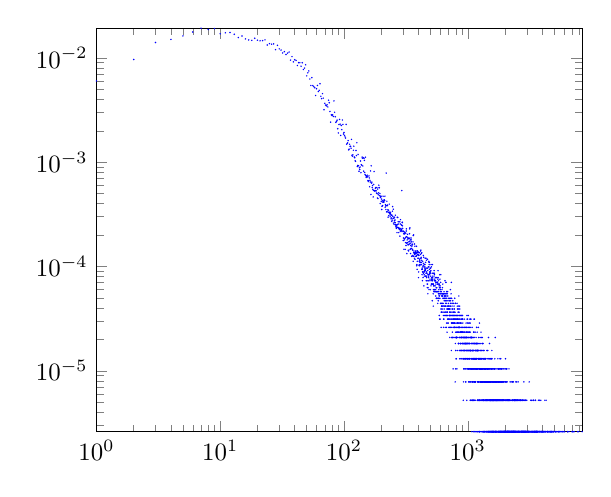
\begin{tikzpicture}
[every mark/.append style={scale=0.1},%
 scale=0.9]
\begin{loglogaxis}[%
  enlargelimits=false%
]
\addplot+[only marks] coordinates
{
  (0, 0.00370399332707742)
  (1, 0.00601084349911400)
  (2, 0.00965227817745881)
  (3, 0.0140392034198742)
  (4, 0.0150453550203331)
  (5, 0.0162470023980833)
  (6, 0.0177327703054967)
  (7, 0.0192758836409155)
  (8, 0.0187311020748639)
  (9, 0.0191012407465353)
  (10, 0.0170055260139733)
  (11, 0.0174173704514668)
  (12, 0.0175346679178415)
  (13, 0.0168517360025042)
  (14, 0.0156605150662095)
  (15, 0.0162157230737167)
  (16, 0.0152043582525300)
  (17, 0.0148681055155891)
  (18, 0.0147325617766671)
  (19, 0.0154363465749156)
  (20, 0.0147899072046726)
  (21, 0.0145839849859258)
  (22, 0.0146465436346590)
  (23, 0.0148837451777724)
  (24, 0.0132963194661675)
  (25, 0.0136925242414777)
  (26, 0.0135387342300086)
  (27, 0.0136117193201974)
  (28, 0.0119956208945898)
  (29, 0.0132103013241594)
  (30, 0.0122015431133366)
  (31, 0.0118913564800345)
  (32, 0.0111588989677833)
  (33, 0.0114769054321770)
  (34, 0.0107705140235647)
  (35, 0.0111197998123250)
  (36, 0.0113700344072578)
  (37, 0.00951934104890076)
  (38, 0.0102856844958824)
  (39, 0.00915702220832100)
  (40, 0.00959753935981726)
  (41, 0.00945938901053145)
  (42, 0.00844802418934478)
  (43, 0.00899541236576024)
  (44, 0.00897716609321306)
  (45, 0.00832812011260615)
  (46, 0.00897195287248530)
  (47, 0.00774163278073243)
  (48, 0.00798665415493745)
  (49, 0.00858878114899447)
  (50, 0.00671984151809023)
  (51, 0.00718642477322532)
  (52, 0.00749661140652741)
  (53, 0.00627150453550232)
  (54, 0.00543738921905970)
  (55, 0.00646178709206579)
  (56, 0.00542696277760417)
  (57, 0.00529402564904612)
  (58, 0.00517672818267138)
  (59, 0.00436085913877595)
  (60, 0.00506203732666052)
  (61, 0.00544520905015135)
  (62, 0.00475185069335842)
  (63, 0.00489000104264423)
  (64, 0.00565113126889812)
  (65, 0.00428787404858722)
  (66, 0.00406631216765715)
  (67, 0.00454332186424777)
  (68, 0.00411583776457093)
  (69, 0.00318267125430087)
  (70, 0.00367010739234694)
  (71, 0.00352935043269727)
  (72, 0.00346679178396409)
  (73, 0.00355280992597222)
  (74, 0.00338859347304760)
  (75, 0.00393076842873522)
  (76, 0.00371181315816907)
  (77, 0.00306537378792614)
  (78, 0.00242154102804710)
  (79, 0.00284641851735999)
  (80, 0.00279949953081010)
  (81, 0.00284902512772388)
  (82, 0.00274476071316857)
  (83, 0.00386820978000203)
  (84, 0.00301063497028461)
  (85, 0.00272390783025750)
  (86, 0.00241111458659157)
  (87, 0.00246846001459699)
  (88, 0.00253101866333018)
  (89, 0.00209050151183400)
  (90, 0.00190543217599832)
  (91, 0.00229381712021685)
  (92, 0.00257011781878842)
  (93, 0.00231467000312791)
  (94, 0.00180638098217078)
  (95, 0.00224429152330308)
  (96, 0.00205140235637575)
  (97, 0.00253883849442183)
  (98, 0.00229903034094462)
  (99, 0.00186372641017620)
  (100, 0.00192889166927326)
  (101, 0.00180898759253466)
  (102, 0.00174642894380147)
  (103, 0.00170472317797935)
  (104, 0.00230163695130850)
  (105, 0.00148576790741320)
  (106, 0.00151183401105203)
  (107, 0.00153008028359920)
  (108, 0.00160827859451569)
  (109, 0.00131112501303305)
  (110, 0.00133197789594412)
  (111, 0.00148576790741320)
  (112, 0.00142060264831613)
  (113, 0.00141799603795225)
  (114, 0.00136325722031071)
  (115, 0.00165519758106558)
  (116, 0.00116776144301950)
  (117, 0.00114169533938067)
  (118, 0.00117558127411115)
  (119, 0.00130069857157752)
  (120, 0.00142320925868001)
  (121, 0.00112084245646961)
  (122, 0.00110259618392243)
  (123, 0.00103221770409760)
  (124, 0.00101918465227819)
  (125, 0.00129287874048587)
  (126, 0.00115733500156397)
  (127, 0.00153529350432697)
  (128, 0.000907100406631224)
  (129, 0.000930559899906170)
  (130, 0.00118600771556668)
  (131, 0.000925346679178404)
  (132, 0.000818475654259207)
  (133, 0.000883640913356279)
  (134, 0.000849754978625801)
  (135, 0.000899280575539576)
  (136, 0.00102700448336983)
  (137, 0.000792409550620379)
  (138, 0.000946199562089467)
  (139, 0.000938379730997819)
  (140, 0.00112084245646961)
  (141, 0.00109216974246690)
  (142, 0.000920133458450639)
  (143, 0.00110520279428632)
  (144, 0.000821082264623090)
  (145, 0.00108956313210302)
  (146, 0.00104003753518925)
  (147, 0.000797622771348144)
  (148, 0.000761130226253784)
  (149, 0.00111562923574185)
  (150, 0.000742883953706604)
  (151, 0.000714211239703893)
  (152, 0.000732457512251073)
  (153, 0.000735064122614956)
  (154, 0.000750703784798253)
  (155, 0.000722031070795541)
  (156, 0.000667292253154001)
  (157, 0.000651652590970704)
  (158, 0.000664685642790119)
  (159, 0.000737670732978839)
  (160, 0.000706391408612244)
  (161, 0.000581274111145867)
  (162, 0.000669898863517884)
  (163, 0.000646439370242939)
  (164, 0.000823688874986973)
  (165, 0.000490042748409967)
  (166, 0.000922740068814521)
  (167, 0.000628193097695759)
  (168, 0.000643832759879056)
  (169, 0.000570847669690336)
  (170, 0.000596913773329164)
  (171, 0.000549994786779273)
  (172, 0.000463976644771139)
  (173, 0.000536961734959859)
  (174, 0.000612553435512461)
  (175, 0.000813262433531441)
  (176, 0.000529141903868210)
  (177, 0.000531748514232093)
  (178, 0.000536961734959859)
  (179, 0.000563027838598687)
  (180, 0.000531748514232093)
  (181, 0.000570847669690336)
  (182, 0.000531748514232093)
  (183, 0.000505682410593264)
  (184, 0.000570847669690336)
  (185, 0.000500469189865499)
  (186, 0.000453550203315608)
  (187, 0.000552601397143156)
  (188, 0.000448336982587842)
  (189, 0.000487436138046084)
  (190, 0.000508289020957147)
  (191, 0.000602126994056930)
  (192, 0.000570847669690336)
  (193, 0.000568241059326453)
  (194, 0.000477009696590553)
  (195, 0.000500469189865499)
  (196, 0.000401417996037952)
  (197, 0.000458763424043373)
  (198, 0.000471796475862787)
  (199, 0.000471796475862787)
  (200, 0.000422270878949014)
  (201, 0.000443123761860077)
  (202, 0.000351892399124179)
  (203, 0.000377958502763007)
  (204, 0.000414451047857366)
  (205, 0.000383171723490772)
  (206, 0.000430090710040663)
  (207, 0.000471796475862787)
  (208, 0.000414451047857366)
  (209, 0.000422270878949014)
  (210, 0.000414451047857366)
  (211, 0.000435303930768428)
  (212, 0.000432697320404545)
  (213, 0.000427484099676780)
  (214, 0.000471796475862787)
  (215, 0.000370138671671358)
  (216, 0.000390991554582421)
  (217, 0.000380565113126889)
  (218, 0.000351892399124179)
  (219, 0.000787196329892613)
  (220, 0.000383171723490772)
  (221, 0.000333646126576999)
  (222, 0.000422270878949014)
  (223, 0.000336252736940882)
  (224, 0.000383171723490772)
  (225, 0.000388384944218538)
  (226, 0.000349285788760296)
  (227, 0.000297153581482640)
  (228, 0.000331039516213116)
  (229, 0.000346679178396413)
  (230, 0.000307580022938171)
  (231, 0.000328432905849233)
  (232, 0.000396204775310186)
  (233, 0.000331039516213116)
  (234, 0.000323219685121468)
  (235, 0.000318006464393702)
  (236, 0.000299760191846522)
  (237, 0.000323219685121468)
  (238, 0.000331039516213116)
  (239, 0.000312793243665936)
  (240, 0.000286727140027108)
  (241, 0.000291940360754874)
  (242, 0.000310186633302054)
  (243, 0.000271087477843812)
  (244, 0.000310186633302054)
  (245, 0.000278907308935460)
  (246, 0.000338859347304764)
  (247, 0.000375351892399124)
  (248, 0.000302366802210405)
  (249, 0.000289333750390991)
  (250, 0.000354499009488061)
  (251, 0.000260661036388280)
  (252, 0.000289333750390991)
  (253, 0.000291940360754874)
  (254, 0.000252841205296632)
  (255, 0.000273694088207694)
  (256, 0.000297153581482640)
  (257, 0.000263267646752163)
  (258, 0.000278907308935460)
  (259, 0.000263267646752163)
  (260, 0.000310186633302054)
  (261, 0.000252841205296632)
  (262, 0.000245021374204984)
  (263, 0.000242414763841101)
  (264, 0.000237201543113335)
  (265, 0.000231988322385570)
  (266, 0.000245021374204984)
  (267, 0.000250234594932749)
  (268, 0.000211135439474507)
  (269, 0.000297153581482640)
  (270, 0.000252841205296632)
  (271, 0.000237201543113335)
  (272, 0.000294546971118757)
  (273, 0.000237201543113335)
  (274, 0.000268480867479929)
  (275, 0.000255447815660515)
  (276, 0.000234594932749452)
  (277, 0.000211135439474507)
  (278, 0.000229381712021687)
  (279, 0.000231988322385570)
  (280, 0.000231988322385570)
  (281, 0.000226775101657804)
  (282, 0.000268480867479929)
  (283, 0.000195495777291210)
  (284, 0.000218955270566156)
  (285, 0.000255447815660515)
  (286, 0.000281513919299343)
  (287, 0.000224168491293921)
  (288, 0.000231988322385570)
  (289, 0.000216348660202273)
  (290, 0.000221561880930038)
  (291, 0.000250234594932749)
  (292, 0.000226775101657804)
  (293, 0.000534355124595976)
  (294, 0.000247627984568866)
  (295, 0.000265874257116046)
  (296, 0.000263267646752163)
  (297, 0.000245021374204984)
  (298, 0.000231988322385570)
  (299, 0.000216348660202273)
  (300, 0.000218955270566156)
  (301, 0.000177249504744031)
  (302, 0.000187675946199562)
  (303, 0.000216348660202273)
  (304, 0.000205922218746742)
  (305, 0.000145970180377437)
  (306, 0.000185069335835679)
  (307, 0.000205922218746742)
  (308, 0.000179856115107913)
  (309, 0.000213742049838390)
  (310, 0.000205922218746742)
  (311, 0.000211135439474507)
  (312, 0.000145970180377437)
  (313, 0.000187675946199562)
  (314, 0.000169429673652382)
  (315, 0.000190282556563445)
  (316, 0.000208528829110624)
  (317, 0.000159003232196851)
  (318, 0.000218955270566156)
  (319, 0.000229381712021687)
  (320, 0.000192889166927327)
  (321, 0.000166823063288499)
  (322, 0.000132937128558023)
  (323, 0.000169429673652382)
  (324, 0.000179856115107913)
  (325, 0.000169429673652382)
  (326, 0.000203315608382859)
  (327, 0.000190282556563445)
  (328, 0.000161609842560734)
  (329, 0.000185069335835679)
  (330, 0.000143363570013554)
  (331, 0.000185069335835679)
  (332, 0.000161609842560734)
  (333, 0.000140756959649671)
  (334, 0.000172036284016265)
  (335, 0.000187675946199562)
  (336, 0.000185069335835679)
  (337, 0.000164216452924617)
  (338, 0.000205922218746742)
  (339, 0.000229381712021687)
  (340, 0.000174642894380148)
  (341, 0.000234594932749452)
  (342, 0.000145970180377437)
  (343, 0.000166823063288499)
  (344, 0.000179856115107913)
  (345, 0.000132937128558023)
  (346, 0.000159003232196851)
  (347, 0.000148576790741320)
  (348, 0.000187675946199562)
  (349, 0.000179856115107913)
  (350, 0.000172036284016265)
  (351, 0.000148576790741320)
  (352, 0.000125117297466375)
  (353, 0.000156396621832968)
  (354, 0.000125117297466375)
  (355, 0.000164216452924617)
  (356, 0.000161609842560734)
  (357, 0.000161609842560734)
  (358, 0.000145970180377437)
  (359, 0.000143363570013554)
  (360, 0.000127723907830257)
  (361, 0.000172036284016265)
  (362, 0.000112084245646961)
  (363, 0.000198102387655093)
  (364, 0.000125117297466375)
  (365, 0.000200708998018976)
  (366, 0.000135543738921906)
  (367, 0.000140756959649671)
  (368, 0.000135543738921906)
  (369, 0.000135543738921906)
  (370, 0.000119904076738609)
  (371, 0.000164216452924617)
  (372, 0.000132937128558023)
  (373, 0.000130330518194140)
  (374, 0.000156396621832968)
  (375, 0.000117297466374726)
  (376, 0.000125117297466375)
  (377, 0.000140756959649671)
  (378, 0.000138150349285789)
  (379, 0.000132937128558023)
  (380, 0.000135543738921906)
  (381, 0.000135543738921906)
  (382, 0.000132937128558023)
  (383, 0.000125117297466375)
  (384, 0.000135543738921906)
  (385, 0.000156396621832968)
  (386, 0.000127723907830257)
  (387, 0.000101657804191429)
  (388, 0.000104264414555312)
  (389, 0.000140756959649671)
  (390, 0.0000938379730997810)
  (391, 0.000112084245646961)
  (392, 0.000140756959649671)
  (393, 0.000135543738921906)
  (394, 0.000130330518194140)
  (395, 0.000119904076738609)
  (396, 0.000130330518194140)
  (397, 0.000138150349285789)
  (398, 0.000119904076738609)
  (399, 0.000127723907830257)
  (400, 0.0000781983109164841)
  (401, 0.0000886247523720154)
  (402, 0.000135543738921906)
  (403, 0.000127723907830257)
  (404, 0.000101657804191429)
  (405, 0.000112084245646961)
  (406, 0.000104264414555312)
  (407, 0.000135543738921906)
  (408, 0.000117297466374726)
  (409, 0.000114690856010843)
  (410, 0.000101657804191429)
  (411, 0.000109477635283078)
  (412, 0.000119904076738609)
  (413, 0.000109477635283078)
  (414, 0.000130330518194140)
  (415, 0.000140756959649671)
  (416, 0.000109477635283078)
  (417, 0.000104264414555312)
  (418, 0.000143363570013554)
  (419, 0.000119904076738609)
  (420, 0.000122510687102492)
  (421, 0.000132937128558023)
  (422, 0.000104264414555312)
  (423, 0.000109477635283078)
  (424, 0.000114690856010843)
  (425, 0.000135543738921906)
  (426, 0.0000938379730997810)
  (427, 0.0000834115316442497)
  (428, 0.0000964445834636638)
  (429, 0.0000938379730997810)
  (430, 0.0000729850901887185)
  (431, 0.0000886247523720154)
  (432, 0.000112084245646961)
  (433, 0.0000886247523720154)
  (434, 0.0000990511938275466)
  (435, 0.0000781983109164841)
  (436, 0.000101657804191429)
  (437, 0.000127723907830257)
  (438, 0.0000860181420081326)
  (439, 0.000106871024919195)
  (440, 0.0000886247523720154)
  (441, 0.000122510687102492)
  (442, 0.0000651652590970701)
  (443, 0.0000990511938275466)
  (444, 0.0000834115316442497)
  (445, 0.0000808049212803669)
  (446, 0.000104264414555312)
  (447, 0.0000912313627358982)
  (448, 0.0000886247523720154)
  (449, 0.0000964445834636638)
  (450, 0.0000990511938275466)
  (451, 0.000104264414555312)
  (452, 0.0000938379730997810)
  (453, 0.000119904076738609)
  (454, 0.0000912313627358982)
  (455, 0.0000938379730997810)
  (456, 0.000109477635283078)
  (457, 0.0000808049212803669)
  (458, 0.0000964445834636638)
  (459, 0.0000808049212803669)
  (460, 0.0000860181420081326)
  (461, 0.000119904076738609)
  (462, 0.0000729850901887185)
  (463, 0.000114690856010843)
  (464, 0.0000886247523720154)
  (465, 0.0000781983109164841)
  (466, 0.0000808049212803669)
  (467, 0.0000964445834636638)
  (468, 0.0000860181420081326)
  (469, 0.0000729850901887185)
  (470, 0.0000677718694609529)
  (471, 0.0000625586487331873)
  (472, 0.000117297466374726)
  (473, 0.0000677718694609529)
  (474, 0.0000964445834636638)
  (475, 0.0000912313627358982)
  (476, 0.0000547388176415389)
  (477, 0.0000834115316442497)
  (478, 0.0000625586487331873)
  (479, 0.0000729850901887185)
  (480, 0.0000990511938275466)
  (481, 0.0000834115316442497)
  (482, 0.0000781983109164841)
  (483, 0.0000808049212803669)
  (484, 0.000112084245646961)
  (485, 0.0000990511938275466)
  (486, 0.0000599520383693045)
  (487, 0.000109477635283078)
  (488, 0.000104264414555312)
  (489, 0.000109477635283078)
  (490, 0.0000938379730997810)
  (491, 0.0000860181420081326)
  (492, 0.0000834115316442497)
  (493, 0.0000886247523720154)
  (494, 0.0000729850901887185)
  (495, 0.0000755917005526013)
  (496, 0.0000886247523720154)
  (497, 0.0000964445834636638)
  (498, 0.0000599520383693045)
  (499, 0.0000886247523720154)
  (500, 0.0000808049212803669)
  (501, 0.0000964445834636638)
  (502, 0.0000860181420081326)
  (503, 0.0000912313627358982)
  (504, 0.0000651652590970701)
  (505, 0.000104264414555312)
  (506, 0.0000729850901887185)
  (507, 0.0000677718694609529)
  (508, 0.0000990511938275466)
  (509, 0.0000755917005526013)
  (510, 0.0000781983109164841)
  (511, 0.0000677718694609529)
  (512, 0.0000677718694609529)
  (513, 0.0000755917005526013)
  (514, 0.0000755917005526013)
  (515, 0.0000677718694609529)
  (516, 0.0000808049212803669)
  (517, 0.0000469189865498905)
  (518, 0.000104264414555312)
  (519, 0.0000729850901887185)
  (520, 0.0000781983109164841)
  (521, 0.0000860181420081326)
  (522, 0.0000755917005526013)
  (523, 0.0000677718694609529)
  (524, 0.0000677718694609529)
  (525, 0.0000547388176415389)
  (526, 0.0000417057658221249)
  (527, 0.0000677718694609529)
  (528, 0.0000599520383693045)
  (529, 0.0000860181420081326)
  (530, 0.0000651652590970701)
  (531, 0.0000599520383693045)
  (532, 0.0000573454280054217)
  (533, 0.0000808049212803669)
  (534, 0.0000912313627358982)
  (535, 0.0000651652590970701)
  (536, 0.0000860181420081326)
  (537, 0.0000729850901887185)
  (538, 0.0000834115316442497)
  (539, 0.0000599520383693045)
  (540, 0.0000599520383693045)
  (541, 0.0000755917005526013)
  (542, 0.0000573454280054217)
  (543, 0.0000573454280054217)
  (544, 0.0000729850901887185)
  (545, 0.0000729850901887185)
  (546, 0.0000651652590970701)
  (547, 0.0000781983109164841)
  (548, 0.0000573454280054217)
  (549, 0.0000729850901887185)
  (550, 0.0000599520383693045)
  (551, 0.0000521322072776561)
  (552, 0.0000703784798248357)
  (553, 0.0000677718694609529)
  (554, 0.0000781983109164841)
  (555, 0.0000625586487331873)
  (556, 0.0000703784798248357)
  (557, 0.0000495255969137733)
  (558, 0.0000495255969137733)
  (559, 0.0000573454280054217)
  (560, 0.0000573454280054217)
  (561, 0.0000625586487331873)
  (562, 0.0000703784798248357)
  (563, 0.0000781983109164841)
  (564, 0.0000781983109164841)
  (565, 0.0000703784798248357)
  (566, 0.0000573454280054217)
  (567, 0.0000495255969137733)
  (568, 0.0000703784798248357)
  (569, 0.0000703784798248357)
  (570, 0.0000573454280054217)
  (571, 0.0000677718694609529)
  (572, 0.0000443123761860077)
  (573, 0.0000755917005526013)
  (574, 0.0000677718694609529)
  (575, 0.0000912313627358982)
  (576, 0.0000781983109164841)
  (577, 0.0000469189865498905)
  (578, 0.0000495255969137733)
  (579, 0.0000573454280054217)
  (580, 0.0000547388176415389)
  (581, 0.0000729850901887185)
  (582, 0.0000677718694609529)
  (583, 0.0000599520383693045)
  (584, 0.0000547388176415389)
  (585, 0.0000495255969137733)
  (586, 0.0000521322072776561)
  (587, 0.0000651652590970701)
  (588, 0.0000338859347304765)
  (589, 0.0000677718694609529)
  (590, 0.0000521322072776561)
  (591, 0.0000625586487331873)
  (592, 0.0000312793243665937)
  (593, 0.0000834115316442497)
  (594, 0.0000547388176415389)
  (595, 0.0000495255969137733)
  (596, 0.0000755917005526013)
  (597, 0.0000651652590970701)
  (598, 0.0000312793243665937)
  (599, 0.0000573454280054217)
  (600, 0.0000625586487331873)
  (601, 0.0000599520383693045)
  (602, 0.0000443123761860077)
  (603, 0.0000547388176415389)
  (604, 0.0000703784798248357)
  (605, 0.0000834115316442497)
  (606, 0.0000443123761860077)
  (607, 0.0000390991554582421)
  (608, 0.0000573454280054217)
  (609, 0.0000260661036388281)
  (610, 0.0000573454280054217)
  (611, 0.0000364925450943593)
  (612, 0.0000364925450943593)
  (613, 0.0000443123761860077)
  (614, 0.0000521322072776561)
  (615, 0.0000417057658221249)
  (616, 0.0000547388176415389)
  (617, 0.0000417057658221249)
  (618, 0.0000390991554582421)
  (619, 0.0000599520383693045)
  (620, 0.0000417057658221249)
  (621, 0.0000364925450943593)
  (622, 0.0000521322072776561)
  (623, 0.0000443123761860077)
  (624, 0.0000625586487331873)
  (625, 0.0000521322072776561)
  (626, 0.0000547388176415389)
  (627, 0.0000547388176415389)
  (628, 0.0000677718694609529)
  (629, 0.0000390991554582421)
  (630, 0.0000495255969137733)
  (631, 0.0000417057658221249)
  (632, 0.0000547388176415389)
  (633, 0.0000443123761860077)
  (634, 0.0000547388176415389)
  (635, 0.0000338859347304765)
  (636, 0.0000495255969137733)
  (637, 0.0000260661036388281)
  (638, 0.0000312793243665937)
  (639, 0.0000547388176415389)
  (640, 0.0000364925450943593)
  (641, 0.0000312793243665937)
  (642, 0.0000417057658221249)
  (643, 0.0000573454280054217)
  (644, 0.0000547388176415389)
  (645, 0.0000469189865498905)
  (646, 0.0000521322072776561)
  (647, 0.0000390991554582421)
  (648, 0.0000495255969137733)
  (649, 0.0000417057658221249)
  (650, 0.0000338859347304765)
  (651, 0.0000521322072776561)
  (652, 0.0000495255969137733)
  (653, 0.0000547388176415389)
  (654, 0.0000364925450943593)
  (655, 0.0000729850901887185)
  (656, 0.0000364925450943593)
  (657, 0.0000260661036388281)
  (658, 0.0000547388176415389)
  (659, 0.0000495255969137733)
  (660, 0.0000521322072776561)
  (661, 0.0000469189865498905)
  (662, 0.0000417057658221249)
  (663, 0.0000443123761860077)
  (664, 0.0000338859347304765)
  (665, 0.0000703784798248357)
  (666, 0.0000417057658221249)
  (667, 0.0000703784798248357)
  (668, 0.0000521322072776561)
  (669, 0.0000364925450943593)
  (670, 0.0000443123761860077)
  (671, 0.0000547388176415389)
  (672, 0.0000260661036388281)
  (673, 0.0000338859347304765)
  (674, 0.0000286727140027109)
  (675, 0.0000573454280054217)
  (676, 0.0000495255969137733)
  (677, 0.0000469189865498905)
  (678, 0.0000573454280054217)
  (679, 0.0000390991554582421)
  (680, 0.0000234594932749453)
  (681, 0.0000364925450943593)
  (682, 0.0000338859347304765)
  (683, 0.0000547388176415389)
  (684, 0.0000364925450943593)
  (685, 0.0000390991554582421)
  (686, 0.0000312793243665937)
  (687, 0.0000573454280054217)
  (688, 0.0000417057658221249)
  (689, 0.0000521322072776561)
  (690, 0.0000286727140027109)
  (691, 0.0000312793243665937)
  (692, 0.0000469189865498905)
  (693, 0.0000417057658221249)
  (694, 0.0000286727140027109)
  (695, 0.0000390991554582421)
  (696, 0.0000417057658221249)
  (697, 0.0000443123761860077)
  (698, 0.0000390991554582421)
  (699, 0.0000390991554582421)
  (700, 0.0000390991554582421)
  (701, 0.0000495255969137733)
  (702, 0.0000260661036388281)
  (703, 0.0000312793243665937)
  (704, 0.0000312793243665937)
  (705, 0.0000417057658221249)
  (706, 0.0000312793243665937)
  (707, 0.0000338859347304765)
  (708, 0.0000390991554582421)
  (709, 0.0000390991554582421)
  (710, 0.0000338859347304765)
  (711, 0.0000495255969137733)
  (712, 0.0000338859347304765)
  (713, 0.0000364925450943593)
  (714, 0.0000260661036388281)
  (715, 0.0000469189865498905)
  (716, 0.0000208528829110625)
  (717, 0.0000469189865498905)
  (718, 0.0000417057658221249)
  (719, 0.0000364925450943593)
  (720, 0.0000390991554582421)
  (721, 0.0000364925450943593)
  (722, 0.0000312793243665937)
  (723, 0.0000417057658221249)
  (724, 0.0000599520383693045)
  (725, 0.0000338859347304765)
  (726, 0.0000443123761860077)
  (727, 0.0000469189865498905)
  (728, 0.0000260661036388281)
  (729, 0.0000260661036388281)
  (730, 0.0000495255969137733)
  (731, 0.0000495255969137733)
  (732, 0.0000443123761860077)
  (733, 0.0000547388176415389)
  (734, 0.0000312793243665937)
  (735, 0.0000338859347304765)
  (736, 0.0000703784798248357)
  (737, 0.0000156396621832968)
  (738, 0.0000286727140027109)
  (739, 0.0000260661036388281)
  (740, 0.0000208528829110625)
  (741, 0.0000495255969137733)
  (742, 0.0000286727140027109)
  (743, 0.0000312793243665937)
  (744, 0.0000364925450943593)
  (745, 0.0000208528829110625)
  (746, 0.0000417057658221249)
  (747, 0.0000208528829110625)
  (748, 0.0000390991554582421)
  (749, 0.0000286727140027109)
  (750, 0.0000390991554582421)
  (751, 0.0000234594932749453)
  (752, 0.0000312793243665937)
  (753, 0.0000286727140027109)
  (754, 0.0000208528829110625)
  (755, 0.0000443123761860077)
  (756, 0.0000338859347304765)
  (757, 0.0000469189865498905)
  (758, 0.0000338859347304765)
  (759, 0.0000208528829110625)
  (760, 0.0000364925450943593)
  (761, 0.0000104264414555312)
  (762, 0.0000260661036388281)
  (763, 0.0000260661036388281)
  (764, 0.0000338859347304765)
  (765, 0.0000286727140027109)
  (766, 0.0000364925450943593)
  (767, 0.0000443123761860077)
  (768, 0.0000286727140027109)
  (769, 0.0000312793243665937)
  (770, 0.0000312793243665937)
  (771, 0.0000312793243665937)
  (772, 0.0000338859347304765)
  (773, 0.0000364925450943593)
  (774, 0.0000417057658221249)
  (775, 0.0000208528829110625)
  (776, 0.0000390991554582421)
  (777, 0.0000364925450943593)
  (778, 0.0000390991554582421)
  (779, 0.0000260661036388281)
  (780, 0.0000286727140027109)
  (781, 0.0000338859347304765)
  (782, 0.0000312793243665937)
  (783, 0.0000286727140027109)
  (784, 0.0000260661036388281)
  (785, 0.0000495255969137733)
  (786, 0.0000260661036388281)
  (787, 0.0000312793243665937)
  (788, 0.0000286727140027109)
  (789, 0.0000364925450943593)
  (790, 0.0000260661036388281)
  (791, 7.81983109164842e-6)
  (792, 0.0000208528829110625)
  (793, 0.0000443123761860077)
  (794, 0.0000182462725471796)
  (795, 0.0000443123761860077)
  (796, 0.0000312793243665937)
  (797, 0.0000104264414555312)
  (798, 0.0000156396621832968)
  (799, 0.0000234594932749453)
  (800, 0.0000338859347304765)
  (801, 0.0000156396621832968)
  (802, 0.0000312793243665937)
  (803, 0.0000208528829110625)
  (804, 0.0000130330518194140)
  (805, 0.0000286727140027109)
  (806, 0.0000338859347304765)
  (807, 0.0000208528829110625)
  (808, 0.0000130330518194140)
  (809, 0.0000312793243665937)
  (810, 0.0000208528829110625)
  (811, 0.0000208528829110625)
  (812, 0.0000260661036388281)
  (813, 0.0000234594932749453)
  (814, 0.0000208528829110625)
  (815, 0.0000208528829110625)
  (816, 0.0000338859347304765)
  (817, 0.0000104264414555312)
  (818, 0.0000312793243665937)
  (819, 0.0000443123761860077)
  (820, 0.0000260661036388281)
  (821, 0.0000234594932749453)
  (822, 0.0000417057658221249)
  (823, 0.0000312793243665937)
  (824, 0.0000286727140027109)
  (825, 0.0000390991554582421)
  (826, 0.0000234594932749453)
  (827, 0.0000312793243665937)
  (828, 0.0000156396621832968)
  (829, 0.0000286727140027109)
  (830, 0.0000338859347304765)
  (831, 0.0000208528829110625)
  (832, 0.0000286727140027109)
  (833, 0.0000364925450943593)
  (834, 0.0000338859347304765)
  (835, 0.0000260661036388281)
  (836, 0.0000312793243665937)
  (837, 0.0000390991554582421)
  (838, 0.0000417057658221249)
  (839, 0.0000286727140027109)
  (840, 0.0000182462725471796)
  (841, 0.0000182462725471796)
  (842, 0.0000234594932749453)
  (843, 0.0000260661036388281)
  (844, 0.0000260661036388281)
  (845, 0.0000182462725471796)
  (846, 0.0000364925450943593)
  (847, 0.0000521322072776561)
  (848, 0.0000234594932749453)
  (849, 0.0000364925450943593)
  (850, 0.0000312793243665937)
  (851, 0.0000312793243665937)
  (852, 0.0000208528829110625)
  (853, 0.0000260661036388281)
  (854, 0.0000286727140027109)
  (855, 0.0000156396621832968)
  (856, 0.0000260661036388281)
  (857, 0.0000208528829110625)
  (858, 0.0000260661036388281)
  (859, 0.0000417057658221249)
  (860, 0.0000130330518194140)
  (861, 0.0000338859347304765)
  (862, 0.0000390991554582421)
  (863, 0.0000338859347304765)
  (864, 0.0000260661036388281)
  (865, 0.0000234594932749453)
  (866, 0.0000156396621832968)
  (867, 0.0000312793243665937)
  (868, 0.0000182462725471796)
  (869, 0.0000234594932749453)
  (870, 0.0000156396621832968)
  (871, 0.0000286727140027109)
  (872, 0.0000234594932749453)
  (873, 0.0000234594932749453)
  (874, 0.0000286727140027109)
  (875, 0.0000182462725471796)
  (876, 0.0000182462725471796)
  (877, 0.0000338859347304765)
  (878, 0.0000208528829110625)
  (879, 0.0000130330518194140)
  (880, 0.0000208528829110625)
  (881, 0.0000234594932749453)
  (882, 0.0000182462725471796)
  (883, 0.0000260661036388281)
  (884, 0.0000286727140027109)
  (885, 0.0000130330518194140)
  (886, 0.0000156396621832968)
  (887, 0.0000312793243665937)
  (888, 0.0000208528829110625)
  (889, 0.0000208528829110625)
  (890, 0.0000338859347304765)
  (891, 0.0000234594932749453)
  (892, 0.0000156396621832968)
  (893, 0.0000208528829110625)
  (894, 0.0000234594932749453)
  (895, 0.0000234594932749453)
  (896, 0.0000234594932749453)
  (897, 0.0000260661036388281)
  (898, 0.0000156396621832968)
  (899, 0.0000312793243665937)
  (900, 0.0000182462725471796)
  (901, 0.0000312793243665937)
  (902, 0.0000234594932749453)
  (903, 0.0000182462725471796)
  (904, 0.0000234594932749453)
  (905, 0.0000312793243665937)
  (906, 0.0000338859347304765)
  (907, 0.0000182462725471796)
  (908, 0.0000260661036388281)
  (909, 0.0000208528829110625)
  (910, 0.0000234594932749453)
  (911, 0.0000286727140027109)
  (912, 0.0000130330518194140)
  (913, 0.0000312793243665937)
  (914, 0.0000156396621832968)
  (915, 0.0000208528829110625)
  (916, 0.0000208528829110625)
  (917, 0.0000182462725471796)
  (918, 0.0000182462725471796)
  (919, 0.0000156396621832968)
  (920, 5.21322072776561e-6)
  (921, 0.0000208528829110625)
  (922, 0.0000182462725471796)
  (923, 7.81983109164842e-6)
  (924, 0.0000130330518194140)
  (925, 0.0000156396621832968)
  (926, 0.0000130330518194140)
  (927, 0.0000208528829110625)
  (928, 0.0000104264414555312)
  (929, 0.0000104264414555312)
  (930, 0.0000234594932749453)
  (931, 0.0000260661036388281)
  (932, 0.0000130330518194140)
  (933, 0.0000208528829110625)
  (934, 0.0000234594932749453)
  (935, 0.0000234594932749453)
  (936, 0.0000260661036388281)
  (937, 0.0000156396621832968)
  (938, 0.0000156396621832968)
  (939, 0.0000130330518194140)
  (940, 0.0000208528829110625)
  (941, 0.0000312793243665937)
  (942, 0.0000182462725471796)
  (943, 0.0000156396621832968)
  (944, 0.0000182462725471796)
  (945, 0.0000208528829110625)
  (946, 0.0000104264414555312)
  (947, 0.0000182462725471796)
  (948, 0.0000260661036388281)
  (949, 0.0000156396621832968)
  (950, 0.0000182462725471796)
  (951, 0.0000208528829110625)
  (952, 0.0000156396621832968)
  (953, 0.0000130330518194140)
  (954, 0.0000130330518194140)
  (955, 0.0000182462725471796)
  (956, 0.0000182462725471796)
  (957, 0.0000182462725471796)
  (958, 0.0000260661036388281)
  (959, 0.0000208528829110625)
  (960, 0.0000182462725471796)
  (961, 0.0000130330518194140)
  (962, 7.81983109164842e-6)
  (963, 7.81983109164842e-6)
  (964, 0.0000104264414555312)
  (965, 0.0000208528829110625)
  (966, 0.0000234594932749453)
  (967, 0.0000208528829110625)
  (968, 0.0000104264414555312)
  (969, 0.0000286727140027109)
  (970, 0.0000182462725471796)
  (971, 0.0000156396621832968)
  (972, 0.0000156396621832968)
  (973, 0.0000208528829110625)
  (974, 0.0000260661036388281)
  (975, 0.0000208528829110625)
  (976, 0.0000234594932749453)
  (977, 0.0000130330518194140)
  (978, 0.0000182462725471796)
  (979, 0.0000234594932749453)
  (980, 0.0000208528829110625)
  (981, 0.0000182462725471796)
  (982, 5.21322072776561e-6)
  (983, 0.0000208528829110625)
  (984, 0.0000260661036388281)
  (985, 0.0000338859347304765)
  (986, 0.0000182462725471796)
  (987, 0.0000156396621832968)
  (988, 0.0000312793243665937)
  (989, 0.0000208528829110625)
  (990, 0.0000104264414555312)
  (991, 0.0000156396621832968)
  (992, 0.0000130330518194140)
  (993, 0.0000130330518194140)
  (994, 0.0000130330518194140)
  (995, 0.0000182462725471796)
  (996, 0.0000312793243665937)
  (997, 0.0000156396621832968)
  (998, 0.0000286727140027109)
  (999, 0.0000182462725471796)
  (1000, 0.0000104264414555312)
  (1001, 0.0000234594932749453)
  (1002, 0.0000130330518194140)
  (1003, 0.0000260661036388281)
  (1004, 0.0000234594932749453)
  (1005, 0.0000234594932749453)
  (1006, 0.0000182462725471796)
  (1007, 0.0000104264414555312)
  (1008, 0.0000286727140027109)
  (1009, 0.0000208528829110625)
  (1010, 0.0000156396621832968)
  (1011, 0.0000338859347304765)
  (1012, 0.0000104264414555312)
  (1013, 0.0000260661036388281)
  (1014, 0.0000156396621832968)
  (1015, 0.0000130330518194140)
  (1016, 0.0000208528829110625)
  (1017, 0.0000104264414555312)
  (1018, 7.81983109164842e-6)
  (1019, 7.81983109164842e-6)
  (1020, 0.0000130330518194140)
  (1021, 0.0000182462725471796)
  (1022, 0.0000182462725471796)
  (1023, 0.0000182462725471796)
  (1024, 0.0000104264414555312)
  (1025, 0.0000182462725471796)
  (1026, 0.0000234594932749453)
  (1027, 0.0000130330518194140)
  (1028, 0.0000182462725471796)
  (1029, 0.0000286727140027109)
  (1030, 0.0000104264414555312)
  (1031, 0.0000130330518194140)
  (1032, 0.0000156396621832968)
  (1033, 7.81983109164842e-6)
  (1034, 0.0000156396621832968)
  (1035, 0.0000234594932749453)
  (1036, 0.0000260661036388281)
  (1037, 0.0000312793243665937)
  (1038, 0.0000130330518194140)
  (1039, 0.0000208528829110625)
  (1040, 0.0000130330518194140)
  (1041, 0.0000182462725471796)
  (1042, 0.0000208528829110625)
  (1043, 0.0000104264414555312)
  (1044, 5.21322072776561e-6)
  (1045, 0.0000286727140027109)
  (1046, 0.0000234594932749453)
  (1047, 0.0000260661036388281)
  (1048, 0.0000156396621832968)
  (1049, 7.81983109164842e-6)
  (1050, 0.0000156396621832968)
  (1051, 0.0000156396621832968)
  (1052, 0.0000104264414555312)
  (1053, 0.0000156396621832968)
  (1054, 0.0000312793243665937)
  (1055, 0.0000104264414555312)
  (1056, 0.0000208528829110625)
  (1057, 5.21322072776561e-6)
  (1058, 0.0000208528829110625)
  (1059, 0.0000208528829110625)
  (1060, 0.0000312793243665937)
  (1061, 7.81983109164842e-6)
  (1062, 5.21322072776561e-6)
  (1063, 0.0000130330518194140)
  (1064, 0.0000208528829110625)
  (1065, 0.0000104264414555312)
  (1066, 0.0000208528829110625)
  (1067, 0.0000182462725471796)
  (1068, 0.0000104264414555312)
  (1069, 0.0000182462725471796)
  (1070, 0.0000156396621832968)
  (1071, 0.0000104264414555312)
  (1072, 0.0000208528829110625)
  (1073, 0.0000208528829110625)
  (1074, 0.0000130330518194140)
  (1075, 0.0000130330518194140)
  (1076, 0.0000208528829110625)
  (1077, 2.60661036388281e-6)
  (1078, 0.0000104264414555312)
  (1079, 0.0000104264414555312)
  (1080, 5.21322072776561e-6)
  (1081, 0.0000130330518194140)
  (1082, 0.0000130330518194140)
  (1083, 0.0000260661036388281)
  (1084, 7.81983109164842e-6)
  (1085, 5.21322072776561e-6)
  (1086, 7.81983109164842e-6)
  (1087, 0.0000182462725471796)
  (1088, 0.0000156396621832968)
  (1089, 0.0000182462725471796)
  (1090, 0.0000156396621832968)
  (1091, 0.0000208528829110625)
  (1092, 7.81983109164842e-6)
  (1093, 0.0000104264414555312)
  (1094, 0.0000130330518194140)
  (1095, 5.21322072776561e-6)
  (1096, 0.0000104264414555312)
  (1097, 0.0000156396621832968)
  (1098, 0.0000130330518194140)
  (1099, 7.81983109164842e-6)
  (1100, 5.21322072776561e-6)
  (1101, 0.0000156396621832968)
  (1102, 0.0000104264414555312)
  (1103, 5.21322072776561e-6)
  (1104, 0.0000104264414555312)
  (1105, 0.0000104264414555312)
  (1106, 5.21322072776561e-6)
  (1107, 7.81983109164842e-6)
  (1108, 0.0000104264414555312)
  (1109, 0.0000130330518194140)
  (1110, 2.60661036388281e-6)
  (1111, 0.0000130330518194140)
  (1112, 0.0000130330518194140)
  (1113, 0.0000130330518194140)
  (1114, 0.0000156396621832968)
  (1115, 0.0000234594932749453)
  (1116, 0.0000208528829110625)
  (1117, 0.0000182462725471796)
  (1118, 0.0000156396621832968)
  (1119, 5.21322072776561e-6)
  (1120, 0.0000234594932749453)
  (1121, 0.0000182462725471796)
  (1122, 0.0000312793243665937)
  (1123, 0.0000182462725471796)
  (1124, 0.0000104264414555312)
  (1125, 0.0000156396621832968)
  (1126, 0.0000208528829110625)
  (1127, 7.81983109164842e-6)
  (1128, 0.0000182462725471796)
  (1129, 0.0000312793243665937)
  (1130, 2.60661036388281e-6)
  (1131, 7.81983109164842e-6)
  (1132, 7.81983109164842e-6)
  (1133, 0.0000104264414555312)
  (1134, 5.21322072776561e-6)
  (1135, 0.0000130330518194140)
  (1136, 0.0000130330518194140)
  (1137, 0.0000130330518194140)
  (1138, 0.0000104264414555312)
  (1139, 0.0000182462725471796)
  (1140, 0.0000130330518194140)
  (1141, 0.0000130330518194140)
  (1142, 0.0000130330518194140)
  (1143, 0.0000104264414555312)
  (1144, 0.0000104264414555312)
  (1145, 0.0000234594932749453)
  (1146, 7.81983109164842e-6)
  (1147, 7.81983109164842e-6)
  (1148, 7.81983109164842e-6)
  (1149, 0.0000130330518194140)
  (1150, 0.0000104264414555312)
  (1151, 0.0000182462725471796)
  (1152, 7.81983109164842e-6)
  (1153, 0.0000182462725471796)
  (1154, 2.60661036388281e-6)
  (1155, 0.0000104264414555312)
  (1156, 0.0000130330518194140)
  (1157, 5.21322072776561e-6)
  (1158, 7.81983109164842e-6)
  (1159, 0.0000156396621832968)
  (1160, 0.0000156396621832968)
  (1161, 0.0000130330518194140)
  (1162, 0.0000156396621832968)
  (1163, 0.0000156396621832968)
  (1164, 0.0000104264414555312)
  (1165, 0.0000130330518194140)
  (1166, 0.0000130330518194140)
  (1167, 0.0000208528829110625)
  (1168, 0.0000104264414555312)
  (1169, 0.0000130330518194140)
  (1170, 0.0000130330518194140)
  (1171, 0.0000104264414555312)
  (1172, 0.0000156396621832968)
  (1173, 0.0000130330518194140)
  (1174, 0.0000182462725471796)
  (1175, 0.0000182462725471796)
  (1177, 0.0000182462725471796)
  (1178, 0.0000260661036388281)
  (1179, 0.0000104264414555312)
  (1180, 0.0000130330518194140)
  (1181, 2.60661036388281e-6)
  (1182, 0.0000260661036388281)
  (1183, 0.0000104264414555312)
  (1184, 0.0000104264414555312)
  (1185, 0.0000156396621832968)
  (1186, 0.0000104264414555312)
  (1187, 0.0000182462725471796)
  (1188, 0.0000156396621832968)
  (1189, 0.0000156396621832968)
  (1190, 0.0000104264414555312)
  (1191, 0.0000234594932749453)
  (1193, 0.0000104264414555312)
  (1194, 2.60661036388281e-6)
  (1195, 5.21322072776561e-6)
  (1196, 0.0000182462725471796)
  (1197, 0.0000156396621832968)
  (1198, 5.21322072776561e-6)
  (1199, 0.0000156396621832968)
  (1200, 7.81983109164842e-6)
  (1201, 7.81983109164842e-6)
  (1202, 5.21322072776561e-6)
  (1203, 0.0000182462725471796)
  (1204, 0.0000104264414555312)
  (1205, 0.0000104264414555312)
  (1206, 0.0000156396621832968)
  (1207, 5.21322072776561e-6)
  (1208, 2.60661036388281e-6)
  (1209, 0.0000130330518194140)
  (1210, 7.81983109164842e-6)
  (1211, 0.0000156396621832968)
  (1212, 0.0000104264414555312)
  (1213, 0.0000130330518194140)
  (1214, 2.60661036388281e-6)
  (1215, 5.21322072776561e-6)
  (1216, 0.0000260661036388281)
  (1217, 0.0000156396621832968)
  (1218, 0.0000156396621832968)
  (1219, 0.0000130330518194140)
  (1221, 0.0000130330518194140)
  (1222, 7.81983109164842e-6)
  (1223, 0.0000130330518194140)
  (1224, 5.21322072776561e-6)
  (1225, 0.0000208528829110625)
  (1226, 7.81983109164842e-6)
  (1227, 7.81983109164842e-6)
  (1228, 0.0000182462725471796)
  (1229, 0.0000130330518194140)
  (1230, 5.21322072776561e-6)
  (1231, 0.0000104264414555312)
  (1232, 2.60661036388281e-6)
  (1233, 7.81983109164842e-6)
  (1234, 0.0000130330518194140)
  (1235, 5.21322072776561e-6)
  (1236, 0.0000182462725471796)
  (1237, 0.0000104264414555312)
  (1238, 2.60661036388281e-6)
  (1239, 0.0000104264414555312)
  (1240, 0.0000130330518194140)
  (1241, 0.0000104264414555312)
  (1242, 0.0000286727140027109)
  (1243, 5.21322072776561e-6)
  (1244, 0.0000130330518194140)
  (1245, 5.21322072776561e-6)
  (1246, 5.21322072776561e-6)
  (1247, 2.60661036388281e-6)
  (1248, 2.60661036388281e-6)
  (1249, 5.21322072776561e-6)
  (1251, 0.0000130330518194140)
  (1252, 0.0000156396621832968)
  (1253, 0.0000104264414555312)
  (1254, 2.60661036388281e-6)
  (1256, 0.0000130330518194140)
  (1257, 0.0000104264414555312)
  (1258, 0.0000208528829110625)
  (1259, 0.0000104264414555312)
  (1260, 7.81983109164842e-6)
  (1261, 5.21322072776561e-6)
  (1262, 0.0000130330518194140)
  (1263, 5.21322072776561e-6)
  (1264, 7.81983109164842e-6)
  (1265, 0.0000104264414555312)
  (1266, 0.0000130330518194140)
  (1267, 0.0000104264414555312)
  (1268, 0.0000156396621832968)
  (1269, 0.0000104264414555312)
  (1270, 7.81983109164842e-6)
  (1271, 0.0000104264414555312)
  (1272, 7.81983109164842e-6)
  (1273, 2.60661036388281e-6)
  (1274, 0.0000182462725471796)
  (1275, 7.81983109164842e-6)
  (1276, 7.81983109164842e-6)
  (1277, 0.0000130330518194140)
  (1278, 0.0000234594932749453)
  (1279, 7.81983109164842e-6)
  (1280, 0.0000104264414555312)
  (1281, 7.81983109164842e-6)
  (1282, 7.81983109164842e-6)
  (1283, 0.0000104264414555312)
  (1284, 0.0000104264414555312)
  (1285, 0.0000208528829110625)
  (1286, 0.0000156396621832968)
  (1287, 0.0000130330518194140)
  (1288, 7.81983109164842e-6)
  (1289, 0.0000130330518194140)
  (1290, 0.0000130330518194140)
  (1291, 7.81983109164842e-6)
  (1292, 0.0000104264414555312)
  (1293, 5.21322072776561e-6)
  (1294, 0.0000104264414555312)
  (1295, 5.21322072776561e-6)
  (1296, 5.21322072776561e-6)
  (1297, 2.60661036388281e-6)
  (1298, 0.0000104264414555312)
  (1299, 0.0000156396621832968)
  (1300, 0.0000104264414555312)
  (1301, 2.60661036388281e-6)
  (1302, 7.81983109164842e-6)
  (1303, 0.0000104264414555312)
  (1304, 0.0000104264414555312)
  (1305, 7.81983109164842e-6)
  (1306, 0.0000104264414555312)
  (1308, 7.81983109164842e-6)
  (1309, 0.0000182462725471796)
  (1310, 2.60661036388281e-6)
  (1311, 0.0000208528829110625)
  (1312, 0.0000130330518194140)
  (1313, 0.0000182462725471796)
  (1314, 7.81983109164842e-6)
  (1315, 7.81983109164842e-6)
  (1316, 7.81983109164842e-6)
  (1317, 5.21322072776561e-6)
  (1318, 5.21322072776561e-6)
  (1319, 2.60661036388281e-6)
  (1320, 7.81983109164842e-6)
  (1321, 7.81983109164842e-6)
  (1322, 5.21322072776561e-6)
  (1323, 0.0000104264414555312)
  (1324, 0.0000156396621832968)
  (1325, 0.0000104264414555312)
  (1326, 5.21322072776561e-6)
  (1327, 7.81983109164842e-6)
  (1328, 0.0000130330518194140)
  (1329, 0.0000182462725471796)
  (1330, 5.21322072776561e-6)
  (1331, 5.21322072776561e-6)
  (1332, 7.81983109164842e-6)
  (1333, 5.21322072776561e-6)
  (1334, 0.0000104264414555312)
  (1335, 0.0000130330518194140)
  (1336, 2.60661036388281e-6)
  (1337, 0.0000130330518194140)
  (1338, 5.21322072776561e-6)
  (1339, 2.60661036388281e-6)
  (1340, 2.60661036388281e-6)
  (1341, 0.0000156396621832968)
  (1342, 5.21322072776561e-6)
  (1343, 5.21322072776561e-6)
  (1344, 2.60661036388281e-6)
  (1345, 5.21322072776561e-6)
  (1346, 7.81983109164842e-6)
  (1347, 7.81983109164842e-6)
  (1348, 5.21322072776561e-6)
  (1349, 0.0000104264414555312)
  (1351, 0.0000130330518194140)
  (1352, 7.81983109164842e-6)
  (1353, 7.81983109164842e-6)
  (1354, 0.0000104264414555312)
  (1355, 0.0000156396621832968)
  (1356, 5.21322072776561e-6)
  (1357, 0.0000104264414555312)
  (1358, 7.81983109164842e-6)
  (1359, 2.60661036388281e-6)
  (1360, 0.0000104264414555312)
  (1361, 2.60661036388281e-6)
  (1362, 7.81983109164842e-6)
  (1363, 0.0000104264414555312)
  (1364, 7.81983109164842e-6)
  (1365, 2.60661036388281e-6)
  (1366, 0.0000130330518194140)
  (1367, 7.81983109164842e-6)
  (1368, 7.81983109164842e-6)
  (1369, 5.21322072776561e-6)
  (1370, 0.0000130330518194140)
  (1371, 5.21322072776561e-6)
  (1372, 2.60661036388281e-6)
  (1373, 7.81983109164842e-6)
  (1374, 2.60661036388281e-6)
  (1376, 0.0000130330518194140)
  (1377, 0.0000104264414555312)
  (1378, 7.81983109164842e-6)
  (1379, 7.81983109164842e-6)
  (1380, 7.81983109164842e-6)
  (1381, 2.60661036388281e-6)
  (1382, 0.0000104264414555312)
  (1383, 7.81983109164842e-6)
  (1384, 7.81983109164842e-6)
  (1385, 2.60661036388281e-6)
  (1386, 0.0000104264414555312)
  (1387, 7.81983109164842e-6)
  (1388, 0.0000104264414555312)
  (1389, 0.0000104264414555312)
  (1390, 5.21322072776561e-6)
  (1391, 0.0000130330518194140)
  (1393, 0.0000104264414555312)
  (1394, 5.21322072776561e-6)
  (1395, 5.21322072776561e-6)
  (1397, 5.21322072776561e-6)
  (1398, 0.0000130330518194140)
  (1399, 0.0000130330518194140)
  (1400, 7.81983109164842e-6)
  (1401, 0.0000104264414555312)
  (1402, 0.0000104264414555312)
  (1403, 7.81983109164842e-6)
  (1404, 5.21322072776561e-6)
  (1405, 5.21322072776561e-6)
  (1406, 2.60661036388281e-6)
  (1407, 0.0000104264414555312)
  (1408, 7.81983109164842e-6)
  (1409, 7.81983109164842e-6)
  (1410, 5.21322072776561e-6)
  (1411, 7.81983109164842e-6)
  (1412, 7.81983109164842e-6)
  (1413, 5.21322072776561e-6)
  (1414, 5.21322072776561e-6)
  (1415, 2.60661036388281e-6)
  (1416, 7.81983109164842e-6)
  (1417, 5.21322072776561e-6)
  (1418, 2.60661036388281e-6)
  (1419, 2.60661036388281e-6)
  (1421, 7.81983109164842e-6)
  (1422, 7.81983109164842e-6)
  (1423, 7.81983109164842e-6)
  (1425, 5.21322072776561e-6)
  (1426, 0.0000156396621832968)
  (1427, 7.81983109164842e-6)
  (1428, 2.60661036388281e-6)
  (1429, 0.0000104264414555312)
  (1430, 0.0000104264414555312)
  (1431, 5.21322072776561e-6)
  (1432, 5.21322072776561e-6)
  (1433, 2.60661036388281e-6)
  (1435, 5.21322072776561e-6)
  (1436, 0.0000104264414555312)
  (1437, 5.21322072776561e-6)
  (1438, 0.0000156396621832968)
  (1439, 2.60661036388281e-6)
  (1440, 7.81983109164842e-6)
  (1441, 0.0000104264414555312)
  (1442, 0.0000104264414555312)
  (1443, 2.60661036388281e-6)
  (1444, 5.21322072776561e-6)
  (1446, 0.0000130330518194140)
  (1447, 7.81983109164842e-6)
  (1448, 7.81983109164842e-6)
  (1449, 7.81983109164842e-6)
  (1450, 0.0000104264414555312)
  (1451, 7.81983109164842e-6)
  (1452, 0.0000156396621832968)
  (1453, 0.0000104264414555312)
  (1454, 0.0000104264414555312)
  (1455, 5.21322072776561e-6)
  (1456, 2.60661036388281e-6)
  (1457, 5.21322072776561e-6)
  (1459, 5.21322072776561e-6)
  (1460, 2.60661036388281e-6)
  (1461, 7.81983109164842e-6)
  (1462, 2.60661036388281e-6)
  (1463, 2.60661036388281e-6)
  (1464, 2.60661036388281e-6)
  (1465, 0.0000104264414555312)
  (1466, 2.60661036388281e-6)
  (1467, 7.81983109164842e-6)
  (1468, 7.81983109164842e-6)
  (1469, 7.81983109164842e-6)
  (1470, 2.60661036388281e-6)
  (1471, 0.0000208528829110625)
  (1472, 0.0000104264414555312)
  (1473, 5.21322072776561e-6)
  (1475, 7.81983109164842e-6)
  (1476, 5.21322072776561e-6)
  (1477, 7.81983109164842e-6)
  (1478, 0.0000130330518194140)
  (1479, 2.60661036388281e-6)
  (1480, 7.81983109164842e-6)
  (1481, 7.81983109164842e-6)
  (1482, 2.60661036388281e-6)
  (1483, 7.81983109164842e-6)
  (1484, 5.21322072776561e-6)
  (1485, 2.60661036388281e-6)
  (1486, 7.81983109164842e-6)
  (1487, 5.21322072776561e-6)
  (1488, 5.21322072776561e-6)
  (1489, 2.60661036388281e-6)
  (1491, 5.21322072776561e-6)
  (1492, 2.60661036388281e-6)
  (1493, 0.0000130330518194140)
  (1494, 5.21322072776561e-6)
  (1495, 0.0000104264414555312)
  (1496, 2.60661036388281e-6)
  (1497, 7.81983109164842e-6)
  (1498, 0.0000182462725471796)
  (1499, 5.21322072776561e-6)
  (1500, 5.21322072776561e-6)
  (1501, 2.60661036388281e-6)
  (1503, 7.81983109164842e-6)
  (1506, 0.0000104264414555312)
  (1507, 2.60661036388281e-6)
  (1508, 2.60661036388281e-6)
  (1509, 7.81983109164842e-6)
  (1510, 0.0000130330518194140)
  (1512, 7.81983109164842e-6)
  (1513, 0.0000104264414555312)
  (1514, 0.0000104264414555312)
  (1515, 5.21322072776561e-6)
  (1516, 7.81983109164842e-6)
  (1517, 5.21322072776561e-6)
  (1518, 5.21322072776561e-6)
  (1519, 5.21322072776561e-6)
  (1520, 5.21322072776561e-6)
  (1521, 2.60661036388281e-6)
  (1522, 7.81983109164842e-6)
  (1523, 2.60661036388281e-6)
  (1524, 2.60661036388281e-6)
  (1525, 5.21322072776561e-6)
  (1526, 7.81983109164842e-6)
  (1527, 0.0000130330518194140)
  (1528, 5.21322072776561e-6)
  (1530, 7.81983109164842e-6)
  (1531, 5.21322072776561e-6)
  (1532, 2.60661036388281e-6)
  (1533, 7.81983109164842e-6)
  (1534, 2.60661036388281e-6)
  (1535, 5.21322072776561e-6)
  (1536, 7.81983109164842e-6)
  (1539, 7.81983109164842e-6)
  (1540, 2.60661036388281e-6)
  (1541, 5.21322072776561e-6)
  (1542, 2.60661036388281e-6)
  (1543, 2.60661036388281e-6)
  (1544, 5.21322072776561e-6)
  (1545, 7.81983109164842e-6)
  (1546, 0.0000130330518194140)
  (1547, 5.21322072776561e-6)
  (1548, 0.0000104264414555312)
  (1549, 2.60661036388281e-6)
  (1550, 2.60661036388281e-6)
  (1551, 2.60661036388281e-6)
  (1552, 0.0000130330518194140)
  (1553, 2.60661036388281e-6)
  (1554, 5.21322072776561e-6)
  (1555, 5.21322072776561e-6)
  (1556, 7.81983109164842e-6)
  (1557, 0.0000104264414555312)
  (1559, 2.60661036388281e-6)
  (1560, 5.21322072776561e-6)
  (1561, 0.0000104264414555312)
  (1562, 0.0000104264414555312)
  (1564, 2.60661036388281e-6)
  (1565, 0.0000104264414555312)
  (1566, 0.0000156396621832968)
  (1567, 5.21322072776561e-6)
  (1568, 5.21322072776561e-6)
  (1569, 0.0000130330518194140)
  (1571, 2.60661036388281e-6)
  (1572, 5.21322072776561e-6)
  (1573, 7.81983109164842e-6)
  (1574, 5.21322072776561e-6)
  (1576, 2.60661036388281e-6)
  (1577, 5.21322072776561e-6)
  (1578, 2.60661036388281e-6)
  (1579, 2.60661036388281e-6)
  (1580, 5.21322072776561e-6)
  (1581, 7.81983109164842e-6)
  (1583, 7.81983109164842e-6)
  (1584, 5.21322072776561e-6)
  (1585, 5.21322072776561e-6)
  (1586, 2.60661036388281e-6)
  (1587, 2.60661036388281e-6)
  (1588, 0.0000104264414555312)
  (1589, 7.81983109164842e-6)
  (1590, 2.60661036388281e-6)
  (1591, 5.21322072776561e-6)
  (1592, 7.81983109164842e-6)
  (1593, 5.21322072776561e-6)
  (1594, 2.60661036388281e-6)
  (1595, 2.60661036388281e-6)
  (1596, 2.60661036388281e-6)
  (1597, 2.60661036388281e-6)
  (1598, 5.21322072776561e-6)
  (1599, 2.60661036388281e-6)
  (1600, 7.81983109164842e-6)
  (1601, 2.60661036388281e-6)
  (1602, 2.60661036388281e-6)
  (1604, 0.0000104264414555312)
  (1605, 5.21322072776561e-6)
  (1606, 5.21322072776561e-6)
  (1607, 2.60661036388281e-6)
  (1608, 5.21322072776561e-6)
  (1609, 5.21322072776561e-6)
  (1610, 7.81983109164842e-6)
  (1611, 2.60661036388281e-6)
  (1612, 5.21322072776561e-6)
  (1613, 7.81983109164842e-6)
  (1616, 7.81983109164842e-6)
  (1617, 2.60661036388281e-6)
  (1618, 2.60661036388281e-6)
  (1620, 5.21322072776561e-6)
  (1621, 5.21322072776561e-6)
  (1622, 5.21322072776561e-6)
  (1623, 2.60661036388281e-6)
  (1624, 2.60661036388281e-6)
  (1626, 2.60661036388281e-6)
  (1627, 7.81983109164842e-6)
  (1628, 2.60661036388281e-6)
  (1629, 0.0000104264414555312)
  (1630, 2.60661036388281e-6)
  (1631, 5.21322072776561e-6)
  (1632, 0.0000104264414555312)
  (1633, 7.81983109164842e-6)
  (1635, 5.21322072776561e-6)
  (1636, 0.0000104264414555312)
  (1637, 5.21322072776561e-6)
  (1639, 5.21322072776561e-6)
  (1640, 5.21322072776561e-6)
  (1642, 7.81983109164842e-6)
  (1644, 2.60661036388281e-6)
  (1646, 2.60661036388281e-6)
  (1647, 0.0000104264414555312)
  (1648, 7.81983109164842e-6)
  (1649, 0.0000104264414555312)
  (1650, 7.81983109164842e-6)
  (1651, 2.60661036388281e-6)
  (1652, 5.21322072776561e-6)
  (1653, 0.0000130330518194140)
  (1655, 2.60661036388281e-6)
  (1656, 5.21322072776561e-6)
  (1658, 5.21322072776561e-6)
  (1659, 2.60661036388281e-6)
  (1660, 2.60661036388281e-6)
  (1661, 0.0000104264414555312)
  (1662, 2.60661036388281e-6)
  (1663, 2.60661036388281e-6)
  (1664, 7.81983109164842e-6)
  (1665, 2.60661036388281e-6)
  (1666, 5.21322072776561e-6)
  (1667, 0.0000208528829110625)
  (1668, 2.60661036388281e-6)
  (1669, 7.81983109164842e-6)
  (1670, 5.21322072776561e-6)
  (1671, 2.60661036388281e-6)
  (1672, 7.81983109164842e-6)
  (1673, 2.60661036388281e-6)
  (1674, 2.60661036388281e-6)
  (1675, 5.21322072776561e-6)
  (1677, 5.21322072776561e-6)
  (1678, 5.21322072776561e-6)
  (1679, 2.60661036388281e-6)
  (1680, 2.60661036388281e-6)
  (1681, 5.21322072776561e-6)
  (1682, 2.60661036388281e-6)
  (1683, 7.81983109164842e-6)
  (1684, 2.60661036388281e-6)
  (1687, 5.21322072776561e-6)
  (1688, 5.21322072776561e-6)
  (1689, 7.81983109164842e-6)
  (1690, 7.81983109164842e-6)
  (1691, 2.60661036388281e-6)
  (1692, 7.81983109164842e-6)
  (1694, 7.81983109164842e-6)
  (1695, 5.21322072776561e-6)
  (1697, 5.21322072776561e-6)
  (1698, 2.60661036388281e-6)
  (1699, 5.21322072776561e-6)
  (1701, 7.81983109164842e-6)
  (1702, 2.60661036388281e-6)
  (1703, 5.21322072776561e-6)
  (1705, 2.60661036388281e-6)
  (1706, 5.21322072776561e-6)
  (1708, 5.21322072776561e-6)
  (1709, 7.81983109164842e-6)
  (1710, 7.81983109164842e-6)
  (1711, 2.60661036388281e-6)
  (1712, 2.60661036388281e-6)
  (1713, 2.60661036388281e-6)
  (1714, 2.60661036388281e-6)
  (1716, 2.60661036388281e-6)
  (1717, 0.0000104264414555312)
  (1718, 5.21322072776561e-6)
  (1719, 2.60661036388281e-6)
  (1721, 5.21322072776561e-6)
  (1723, 5.21322072776561e-6)
  (1724, 2.60661036388281e-6)
  (1725, 5.21322072776561e-6)
  (1727, 7.81983109164842e-6)
  (1729, 5.21322072776561e-6)
  (1731, 5.21322072776561e-6)
  (1732, 2.60661036388281e-6)
  (1733, 5.21322072776561e-6)
  (1734, 2.60661036388281e-6)
  (1735, 5.21322072776561e-6)
  (1736, 5.21322072776561e-6)
  (1740, 2.60661036388281e-6)
  (1742, 5.21322072776561e-6)
  (1745, 7.81983109164842e-6)
  (1750, 0.0000130330518194140)
  (1751, 7.81983109164842e-6)
  (1752, 7.81983109164842e-6)
  (1753, 5.21322072776561e-6)
  (1754, 0.0000104264414555312)
  (1755, 5.21322072776561e-6)
  (1756, 2.60661036388281e-6)
  (1758, 5.21322072776561e-6)
  (1759, 5.21322072776561e-6)
  (1760, 2.60661036388281e-6)
  (1761, 0.0000104264414555312)
  (1763, 2.60661036388281e-6)
  (1764, 0.0000104264414555312)
  (1765, 7.81983109164842e-6)
  (1766, 2.60661036388281e-6)
  (1767, 2.60661036388281e-6)
  (1768, 2.60661036388281e-6)
  (1769, 7.81983109164842e-6)
  (1770, 2.60661036388281e-6)
  (1771, 2.60661036388281e-6)
  (1772, 5.21322072776561e-6)
  (1773, 2.60661036388281e-6)
  (1774, 7.81983109164842e-6)
  (1775, 5.21322072776561e-6)
  (1777, 2.60661036388281e-6)
  (1779, 5.21322072776561e-6)
  (1780, 5.21322072776561e-6)
  (1781, 2.60661036388281e-6)
  (1782, 0.0000104264414555312)
  (1784, 7.81983109164842e-6)
  (1785, 0.0000104264414555312)
  (1786, 7.81983109164842e-6)
  (1788, 0.0000104264414555312)
  (1789, 7.81983109164842e-6)
  (1790, 5.21322072776561e-6)
  (1791, 5.21322072776561e-6)
  (1792, 5.21322072776561e-6)
  (1794, 2.60661036388281e-6)
  (1795, 7.81983109164842e-6)
  (1797, 7.81983109164842e-6)
  (1798, 2.60661036388281e-6)
  (1800, 5.21322072776561e-6)
  (1801, 2.60661036388281e-6)
  (1802, 5.21322072776561e-6)
  (1803, 5.21322072776561e-6)
  (1804, 0.0000104264414555312)
  (1805, 2.60661036388281e-6)
  (1807, 5.21322072776561e-6)
  (1808, 2.60661036388281e-6)
  (1810, 2.60661036388281e-6)
  (1811, 2.60661036388281e-6)
  (1812, 2.60661036388281e-6)
  (1814, 5.21322072776561e-6)
  (1815, 2.60661036388281e-6)
  (1817, 2.60661036388281e-6)
  (1818, 5.21322072776561e-6)
  (1819, 7.81983109164842e-6)
  (1820, 2.60661036388281e-6)
  (1821, 2.60661036388281e-6)
  (1822, 0.0000130330518194140)
  (1823, 5.21322072776561e-6)
  (1824, 5.21322072776561e-6)
  (1825, 2.60661036388281e-6)
  (1826, 5.21322072776561e-6)
  (1828, 2.60661036388281e-6)
  (1829, 0.0000104264414555312)
  (1830, 2.60661036388281e-6)
  (1831, 5.21322072776561e-6)
  (1834, 2.60661036388281e-6)
  (1835, 2.60661036388281e-6)
  (1836, 5.21322072776561e-6)
  (1837, 7.81983109164842e-6)
  (1838, 2.60661036388281e-6)
  (1839, 2.60661036388281e-6)
  (1841, 2.60661036388281e-6)
  (1844, 2.60661036388281e-6)
  (1846, 5.21322072776561e-6)
  (1847, 0.0000130330518194140)
  (1848, 2.60661036388281e-6)
  (1849, 7.81983109164842e-6)
  (1850, 0.0000104264414555312)
  (1851, 2.60661036388281e-6)
  (1852, 2.60661036388281e-6)
  (1853, 7.81983109164842e-6)
  (1854, 2.60661036388281e-6)
  (1856, 2.60661036388281e-6)
  (1857, 0.0000104264414555312)
  (1858, 2.60661036388281e-6)
  (1859, 7.81983109164842e-6)
  (1860, 5.21322072776561e-6)
  (1861, 7.81983109164842e-6)
  (1864, 2.60661036388281e-6)
  (1865, 7.81983109164842e-6)
  (1869, 2.60661036388281e-6)
  (1870, 0.0000104264414555312)
  (1871, 2.60661036388281e-6)
  (1872, 2.60661036388281e-6)
  (1874, 0.0000104264414555312)
  (1875, 2.60661036388281e-6)
  (1877, 5.21322072776561e-6)
  (1879, 5.21322072776561e-6)
  (1880, 2.60661036388281e-6)
  (1881, 2.60661036388281e-6)
  (1882, 5.21322072776561e-6)
  (1883, 5.21322072776561e-6)
  (1884, 2.60661036388281e-6)
  (1886, 2.60661036388281e-6)
  (1888, 7.81983109164842e-6)
  (1889, 2.60661036388281e-6)
  (1890, 5.21322072776561e-6)
  (1891, 5.21322072776561e-6)
  (1892, 2.60661036388281e-6)
  (1893, 2.60661036388281e-6)
  (1894, 7.81983109164842e-6)
  (1898, 0.0000104264414555312)
  (1901, 7.81983109164842e-6)
  (1903, 2.60661036388281e-6)
  (1904, 5.21322072776561e-6)
  (1906, 2.60661036388281e-6)
  (1907, 2.60661036388281e-6)
  (1908, 2.60661036388281e-6)
  (1909, 5.21322072776561e-6)
  (1910, 2.60661036388281e-6)
  (1911, 5.21322072776561e-6)
  (1913, 5.21322072776561e-6)
  (1915, 2.60661036388281e-6)
  (1917, 7.81983109164842e-6)
  (1918, 5.21322072776561e-6)
  (1921, 2.60661036388281e-6)
  (1922, 2.60661036388281e-6)
  (1925, 5.21322072776561e-6)
  (1926, 2.60661036388281e-6)
  (1928, 5.21322072776561e-6)
  (1929, 7.81983109164842e-6)
  (1930, 5.21322072776561e-6)
  (1931, 2.60661036388281e-6)
  (1933, 5.21322072776561e-6)
  (1937, 2.60661036388281e-6)
  (1938, 2.60661036388281e-6)
  (1940, 2.60661036388281e-6)
  (1941, 0.0000104264414555312)
  (1942, 7.81983109164842e-6)
  (1943, 7.81983109164842e-6)
  (1944, 2.60661036388281e-6)
  (1945, 2.60661036388281e-6)
  (1947, 5.21322072776561e-6)
  (1948, 5.21322072776561e-6)
  (1949, 2.60661036388281e-6)
  (1951, 5.21322072776561e-6)
  (1954, 2.60661036388281e-6)
  (1956, 2.60661036388281e-6)
  (1957, 5.21322072776561e-6)
  (1958, 2.60661036388281e-6)
  (1959, 2.60661036388281e-6)
  (1960, 5.21322072776561e-6)
  (1961, 2.60661036388281e-6)
  (1962, 2.60661036388281e-6)
  (1964, 2.60661036388281e-6)
  (1965, 5.21322072776561e-6)
  (1966, 5.21322072776561e-6)
  (1968, 2.60661036388281e-6)
  (1970, 2.60661036388281e-6)
  (1971, 2.60661036388281e-6)
  (1972, 2.60661036388281e-6)
  (1973, 2.60661036388281e-6)
  (1974, 2.60661036388281e-6)
  (1975, 5.21322072776561e-6)
  (1977, 2.60661036388281e-6)
  (1981, 2.60661036388281e-6)
  (1982, 2.60661036388281e-6)
  (1985, 2.60661036388281e-6)
  (1986, 2.60661036388281e-6)
  (1989, 2.60661036388281e-6)
  (1990, 2.60661036388281e-6)
  (1992, 2.60661036388281e-6)
  (1993, 7.81983109164842e-6)
  (1994, 2.60661036388281e-6)
  (1995, 0.0000104264414555312)
  (1996, 2.60661036388281e-6)
  (1998, 2.60661036388281e-6)
  (1999, 5.21322072776561e-6)
  (2001, 2.60661036388281e-6)
  (2002, 7.81983109164842e-6)
  (2004, 5.21322072776561e-6)
  (2007, 2.60661036388281e-6)
  (2008, 2.60661036388281e-6)
  (2010, 2.60661036388281e-6)
  (2011, 2.60661036388281e-6)
  (2012, 5.21322072776561e-6)
  (2014, 5.21322072776561e-6)
  (2015, 0.0000130330518194140)
  (2018, 2.60661036388281e-6)
  (2019, 7.81983109164842e-6)
  (2021, 2.60661036388281e-6)
  (2022, 2.60661036388281e-6)
  (2025, 2.60661036388281e-6)
  (2026, 2.60661036388281e-6)
  (2027, 2.60661036388281e-6)
  (2029, 5.21322072776561e-6)
  (2030, 2.60661036388281e-6)
  (2031, 5.21322072776561e-6)
  (2033, 2.60661036388281e-6)
  (2034, 2.60661036388281e-6)
  (2035, 0.0000104264414555312)
  (2036, 2.60661036388281e-6)
  (2039, 0.0000104264414555312)
  (2041, 7.81983109164842e-6)
  (2044, 5.21322072776561e-6)
  (2046, 2.60661036388281e-6)
  (2047, 0.0000104264414555312)
  (2048, 5.21322072776561e-6)
  (2049, 2.60661036388281e-6)
  (2050, 2.60661036388281e-6)
  (2054, 2.60661036388281e-6)
  (2055, 2.60661036388281e-6)
  (2056, 2.60661036388281e-6)
  (2057, 2.60661036388281e-6)
  (2059, 5.21322072776561e-6)
  (2063, 2.60661036388281e-6)
  (2065, 5.21322072776561e-6)
  (2066, 2.60661036388281e-6)
  (2070, 0.0000104264414555312)
  (2071, 7.81983109164842e-6)
  (2072, 2.60661036388281e-6)
  (2073, 7.81983109164842e-6)
  (2074, 2.60661036388281e-6)
  (2075, 2.60661036388281e-6)
  (2079, 5.21322072776561e-6)
  (2081, 2.60661036388281e-6)
  (2083, 2.60661036388281e-6)
  (2084, 2.60661036388281e-6)
  (2085, 2.60661036388281e-6)
  (2086, 2.60661036388281e-6)
  (2088, 2.60661036388281e-6)
  (2089, 2.60661036388281e-6)
  (2090, 2.60661036388281e-6)
  (2092, 2.60661036388281e-6)
  (2094, 2.60661036388281e-6)
  (2095, 2.60661036388281e-6)
  (2097, 2.60661036388281e-6)
  (2098, 5.21322072776561e-6)
  (2099, 5.21322072776561e-6)
  (2100, 5.21322072776561e-6)
  (2102, 2.60661036388281e-6)
  (2103, 2.60661036388281e-6)
  (2104, 5.21322072776561e-6)
  (2105, 2.60661036388281e-6)
  (2106, 2.60661036388281e-6)
  (2107, 2.60661036388281e-6)
  (2108, 5.21322072776561e-6)
  (2109, 2.60661036388281e-6)
  (2111, 2.60661036388281e-6)
  (2112, 2.60661036388281e-6)
  (2113, 5.21322072776561e-6)
  (2114, 5.21322072776561e-6)
  (2116, 2.60661036388281e-6)
  (2117, 5.21322072776561e-6)
  (2118, 2.60661036388281e-6)
  (2120, 5.21322072776561e-6)
  (2123, 5.21322072776561e-6)
  (2124, 2.60661036388281e-6)
  (2125, 2.60661036388281e-6)
  (2127, 2.60661036388281e-6)
  (2128, 2.60661036388281e-6)
  (2129, 2.60661036388281e-6)
  (2132, 2.60661036388281e-6)
  (2133, 5.21322072776561e-6)
  (2136, 5.21322072776561e-6)
  (2137, 2.60661036388281e-6)
  (2141, 2.60661036388281e-6)
  (2142, 2.60661036388281e-6)
  (2143, 2.60661036388281e-6)
  (2144, 2.60661036388281e-6)
  (2145, 2.60661036388281e-6)
  (2146, 2.60661036388281e-6)
  (2147, 5.21322072776561e-6)
  (2149, 2.60661036388281e-6)
  (2150, 2.60661036388281e-6)
  (2151, 0.0000104264414555312)
  (2155, 5.21322072776561e-6)
  (2156, 2.60661036388281e-6)
  (2160, 2.60661036388281e-6)
  (2161, 5.21322072776561e-6)
  (2163, 2.60661036388281e-6)
  (2165, 2.60661036388281e-6)
  (2168, 5.21322072776561e-6)
  (2169, 5.21322072776561e-6)
  (2170, 2.60661036388281e-6)
  (2171, 2.60661036388281e-6)
  (2173, 2.60661036388281e-6)
  (2174, 5.21322072776561e-6)
  (2175, 2.60661036388281e-6)
  (2177, 5.21322072776561e-6)
  (2178, 2.60661036388281e-6)
  (2180, 2.60661036388281e-6)
  (2182, 2.60661036388281e-6)
  (2183, 2.60661036388281e-6)
  (2186, 2.60661036388281e-6)
  (2187, 2.60661036388281e-6)
  (2188, 5.21322072776561e-6)
  (2189, 2.60661036388281e-6)
  (2195, 2.60661036388281e-6)
  (2198, 7.81983109164842e-6)
  (2199, 5.21322072776561e-6)
  (2200, 2.60661036388281e-6)
  (2211, 2.60661036388281e-6)
  (2212, 2.60661036388281e-6)
  (2213, 2.60661036388281e-6)
  (2215, 2.60661036388281e-6)
  (2216, 2.60661036388281e-6)
  (2217, 5.21322072776561e-6)
  (2223, 2.60661036388281e-6)
  (2225, 2.60661036388281e-6)
  (2226, 2.60661036388281e-6)
  (2227, 2.60661036388281e-6)
  (2228, 2.60661036388281e-6)
  (2231, 2.60661036388281e-6)
  (2235, 2.60661036388281e-6)
  (2237, 2.60661036388281e-6)
  (2239, 2.60661036388281e-6)
  (2241, 7.81983109164842e-6)
  (2242, 2.60661036388281e-6)
  (2244, 2.60661036388281e-6)
  (2245, 2.60661036388281e-6)
  (2246, 2.60661036388281e-6)
  (2251, 5.21322072776561e-6)
  (2254, 2.60661036388281e-6)
  (2255, 2.60661036388281e-6)
  (2256, 2.60661036388281e-6)
  (2258, 2.60661036388281e-6)
  (2260, 2.60661036388281e-6)
  (2261, 2.60661036388281e-6)
  (2264, 2.60661036388281e-6)
  (2266, 2.60661036388281e-6)
  (2267, 2.60661036388281e-6)
  (2269, 2.60661036388281e-6)
  (2272, 5.21322072776561e-6)
  (2273, 2.60661036388281e-6)
  (2275, 2.60661036388281e-6)
  (2279, 2.60661036388281e-6)
  (2283, 2.60661036388281e-6)
  (2286, 2.60661036388281e-6)
  (2290, 7.81983109164842e-6)
  (2292, 2.60661036388281e-6)
  (2293, 2.60661036388281e-6)
  (2297, 2.60661036388281e-6)
  (2299, 2.60661036388281e-6)
  (2300, 2.60661036388281e-6)
  (2301, 5.21322072776561e-6)
  (2302, 7.81983109164842e-6)
  (2303, 5.21322072776561e-6)
  (2304, 2.60661036388281e-6)
  (2305, 2.60661036388281e-6)
  (2306, 2.60661036388281e-6)
  (2307, 2.60661036388281e-6)
  (2309, 5.21322072776561e-6)
  (2310, 2.60661036388281e-6)
  (2311, 5.21322072776561e-6)
  (2312, 5.21322072776561e-6)
  (2314, 5.21322072776561e-6)
  (2315, 2.60661036388281e-6)
  (2316, 2.60661036388281e-6)
  (2319, 5.21322072776561e-6)
  (2324, 2.60661036388281e-6)
  (2325, 2.60661036388281e-6)
  (2326, 2.60661036388281e-6)
  (2330, 2.60661036388281e-6)
  (2333, 7.81983109164842e-6)
  (2336, 2.60661036388281e-6)
  (2337, 2.60661036388281e-6)
  (2338, 2.60661036388281e-6)
  (2340, 5.21322072776561e-6)
  (2344, 2.60661036388281e-6)
  (2345, 2.60661036388281e-6)
  (2347, 2.60661036388281e-6)
  (2348, 2.60661036388281e-6)
  (2349, 2.60661036388281e-6)
  (2351, 2.60661036388281e-6)
  (2352, 2.60661036388281e-6)
  (2354, 2.60661036388281e-6)
  (2355, 2.60661036388281e-6)
  (2356, 2.60661036388281e-6)
  (2357, 2.60661036388281e-6)
  (2358, 2.60661036388281e-6)
  (2362, 5.21322072776561e-6)
  (2363, 2.60661036388281e-6)
  (2365, 5.21322072776561e-6)
  (2367, 2.60661036388281e-6)
  (2371, 5.21322072776561e-6)
  (2372, 2.60661036388281e-6)
  (2376, 2.60661036388281e-6)
  (2377, 2.60661036388281e-6)
  (2381, 2.60661036388281e-6)
  (2384, 5.21322072776561e-6)
  (2386, 2.60661036388281e-6)
  (2387, 2.60661036388281e-6)
  (2390, 2.60661036388281e-6)
  (2391, 2.60661036388281e-6)
  (2392, 2.60661036388281e-6)
  (2393, 5.21322072776561e-6)
  (2395, 2.60661036388281e-6)
  (2396, 5.21322072776561e-6)
  (2398, 5.21322072776561e-6)
  (2399, 2.60661036388281e-6)
  (2400, 2.60661036388281e-6)
  (2403, 5.21322072776561e-6)
  (2405, 5.21322072776561e-6)
  (2406, 5.21322072776561e-6)
  (2407, 2.60661036388281e-6)
  (2408, 2.60661036388281e-6)
  (2410, 5.21322072776561e-6)
  (2412, 5.21322072776561e-6)
  (2413, 2.60661036388281e-6)
  (2414, 5.21322072776561e-6)
  (2420, 5.21322072776561e-6)
  (2421, 2.60661036388281e-6)
  (2425, 2.60661036388281e-6)
  (2426, 5.21322072776561e-6)
  (2429, 2.60661036388281e-6)
  (2431, 2.60661036388281e-6)
  (2432, 2.60661036388281e-6)
  (2433, 2.60661036388281e-6)
  (2435, 2.60661036388281e-6)
  (2438, 2.60661036388281e-6)
  (2439, 2.60661036388281e-6)
  (2440, 2.60661036388281e-6)
  (2442, 2.60661036388281e-6)
  (2444, 7.81983109164842e-6)
  (2445, 2.60661036388281e-6)
  (2450, 2.60661036388281e-6)
  (2453, 2.60661036388281e-6)
  (2454, 2.60661036388281e-6)
  (2458, 5.21322072776561e-6)
  (2461, 2.60661036388281e-6)
  (2462, 5.21322072776561e-6)
  (2468, 2.60661036388281e-6)
  (2472, 5.21322072776561e-6)
  (2473, 2.60661036388281e-6)
  (2474, 2.60661036388281e-6)
  (2476, 7.81983109164842e-6)
  (2482, 5.21322072776561e-6)
  (2484, 2.60661036388281e-6)
  (2486, 2.60661036388281e-6)
  (2487, 2.60661036388281e-6)
  (2488, 2.60661036388281e-6)
  (2495, 2.60661036388281e-6)
  (2499, 2.60661036388281e-6)
  (2501, 5.21322072776561e-6)
  (2502, 5.21322072776561e-6)
  (2509, 2.60661036388281e-6)
  (2511, 2.60661036388281e-6)
  (2513, 2.60661036388281e-6)
  (2514, 5.21322072776561e-6)
  (2515, 5.21322072776561e-6)
  (2516, 2.60661036388281e-6)
  (2517, 2.60661036388281e-6)
  (2519, 2.60661036388281e-6)
  (2523, 5.21322072776561e-6)
  (2526, 5.21322072776561e-6)
  (2531, 2.60661036388281e-6)
  (2535, 2.60661036388281e-6)
  (2537, 5.21322072776561e-6)
  (2541, 2.60661036388281e-6)
  (2542, 2.60661036388281e-6)
  (2543, 2.60661036388281e-6)
  (2544, 2.60661036388281e-6)
  (2546, 2.60661036388281e-6)
  (2550, 7.81983109164842e-6)
  (2551, 2.60661036388281e-6)
  (2557, 2.60661036388281e-6)
  (2561, 2.60661036388281e-6)
  (2562, 5.21322072776561e-6)
  (2565, 2.60661036388281e-6)
  (2573, 2.60661036388281e-6)
  (2574, 2.60661036388281e-6)
  (2579, 2.60661036388281e-6)
  (2581, 2.60661036388281e-6)
  (2583, 2.60661036388281e-6)
  (2584, 5.21322072776561e-6)
  (2585, 2.60661036388281e-6)
  (2586, 2.60661036388281e-6)
  (2587, 2.60661036388281e-6)
  (2589, 5.21322072776561e-6)
  (2590, 2.60661036388281e-6)
  (2593, 2.60661036388281e-6)
  (2594, 2.60661036388281e-6)
  (2595, 5.21322072776561e-6)
  (2597, 2.60661036388281e-6)
  (2602, 5.21322072776561e-6)
  (2606, 2.60661036388281e-6)
  (2607, 2.60661036388281e-6)
  (2608, 2.60661036388281e-6)
  (2612, 2.60661036388281e-6)
  (2613, 2.60661036388281e-6)
  (2614, 2.60661036388281e-6)
  (2633, 2.60661036388281e-6)
  (2635, 5.21322072776561e-6)
  (2640, 2.60661036388281e-6)
  (2641, 2.60661036388281e-6)
  (2642, 2.60661036388281e-6)
  (2645, 5.21322072776561e-6)
  (2650, 5.21322072776561e-6)
  (2652, 5.21322072776561e-6)
  (2655, 5.21322072776561e-6)
  (2656, 2.60661036388281e-6)
  (2661, 2.60661036388281e-6)
  (2670, 2.60661036388281e-6)
  (2676, 2.60661036388281e-6)
  (2677, 5.21322072776561e-6)
  (2683, 2.60661036388281e-6)
  (2684, 5.21322072776561e-6)
  (2693, 2.60661036388281e-6)
  (2698, 2.60661036388281e-6)
  (2702, 2.60661036388281e-6)
  (2704, 2.60661036388281e-6)
  (2705, 2.60661036388281e-6)
  (2706, 2.60661036388281e-6)
  (2710, 2.60661036388281e-6)
  (2711, 2.60661036388281e-6)
  (2712, 5.21322072776561e-6)
  (2714, 2.60661036388281e-6)
  (2716, 2.60661036388281e-6)
  (2717, 2.60661036388281e-6)
  (2719, 2.60661036388281e-6)
  (2723, 2.60661036388281e-6)
  (2734, 2.60661036388281e-6)
  (2735, 5.21322072776561e-6)
  (2736, 2.60661036388281e-6)
  (2738, 2.60661036388281e-6)
  (2744, 2.60661036388281e-6)
  (2749, 2.60661036388281e-6)
  (2750, 5.21322072776561e-6)
  (2752, 2.60661036388281e-6)
  (2754, 2.60661036388281e-6)
  (2757, 2.60661036388281e-6)
  (2761, 2.60661036388281e-6)
  (2766, 2.60661036388281e-6)
  (2768, 5.21322072776561e-6)
  (2773, 2.60661036388281e-6)
  (2774, 2.60661036388281e-6)
  (2775, 2.60661036388281e-6)
  (2778, 2.60661036388281e-6)
  (2782, 2.60661036388281e-6)
  (2784, 2.60661036388281e-6)
  (2786, 5.21322072776561e-6)
  (2791, 5.21322072776561e-6)
  (2794, 2.60661036388281e-6)
  (2795, 5.21322072776561e-6)
  (2798, 2.60661036388281e-6)
  (2799, 5.21322072776561e-6)
  (2805, 2.60661036388281e-6)
  (2806, 2.60661036388281e-6)
  (2811, 2.60661036388281e-6)
  (2812, 2.60661036388281e-6)
  (2821, 2.60661036388281e-6)
  (2822, 2.60661036388281e-6)
  (2823, 2.60661036388281e-6)
  (2826, 2.60661036388281e-6)
  (2831, 2.60661036388281e-6)
  (2833, 2.60661036388281e-6)
  (2836, 2.60661036388281e-6)
  (2837, 7.81983109164842e-6)
  (2838, 2.60661036388281e-6)
  (2843, 2.60661036388281e-6)
  (2849, 2.60661036388281e-6)
  (2850, 2.60661036388281e-6)
  (2851, 2.60661036388281e-6)
  (2853, 5.21322072776561e-6)
  (2856, 2.60661036388281e-6)
  (2858, 2.60661036388281e-6)
  (2861, 2.60661036388281e-6)
  (2863, 2.60661036388281e-6)
  (2868, 2.60661036388281e-6)
  (2869, 2.60661036388281e-6)
  (2871, 2.60661036388281e-6)
  (2872, 2.60661036388281e-6)
  (2878, 5.21322072776561e-6)
  (2881, 2.60661036388281e-6)
  (2884, 2.60661036388281e-6)
  (2885, 2.60661036388281e-6)
  (2887, 2.60661036388281e-6)
  (2892, 2.60661036388281e-6)
  (2903, 5.21322072776561e-6)
  (2905, 2.60661036388281e-6)
  (2909, 2.60661036388281e-6)
  (2910, 2.60661036388281e-6)
  (2914, 2.60661036388281e-6)
  (2915, 2.60661036388281e-6)
  (2917, 2.60661036388281e-6)
  (2919, 2.60661036388281e-6)
  (2923, 5.21322072776561e-6)
  (2924, 2.60661036388281e-6)
  (2926, 2.60661036388281e-6)
  (2930, 2.60661036388281e-6)
  (2938, 2.60661036388281e-6)
  (2939, 2.60661036388281e-6)
  (2941, 2.60661036388281e-6)
  (2947, 2.60661036388281e-6)
  (2948, 2.60661036388281e-6)
  (2949, 2.60661036388281e-6)
  (2955, 2.60661036388281e-6)
  (2956, 5.21322072776561e-6)
  (2961, 2.60661036388281e-6)
  (2966, 2.60661036388281e-6)
  (2973, 2.60661036388281e-6)
  (2977, 2.60661036388281e-6)
  (2978, 2.60661036388281e-6)
  (2984, 2.60661036388281e-6)
  (2993, 2.60661036388281e-6)
  (2998, 2.60661036388281e-6)
  (3000, 5.21322072776561e-6)
  (3001, 2.60661036388281e-6)
  (3016, 2.60661036388281e-6)
  (3023, 2.60661036388281e-6)
  (3025, 2.60661036388281e-6)
  (3031, 2.60661036388281e-6)
  (3037, 2.60661036388281e-6)
  (3040, 2.60661036388281e-6)
  (3049, 2.60661036388281e-6)
  (3063, 2.60661036388281e-6)
  (3065, 2.60661036388281e-6)
  (3072, 2.60661036388281e-6)
  (3075, 2.60661036388281e-6)
  (3076, 2.60661036388281e-6)
  (3077, 2.60661036388281e-6)
  (3081, 2.60661036388281e-6)
  (3089, 2.60661036388281e-6)
  (3090, 2.60661036388281e-6)
  (3092, 2.60661036388281e-6)
  (3102, 2.60661036388281e-6)
  (3104, 2.60661036388281e-6)
  (3108, 2.60661036388281e-6)
  (3109, 2.60661036388281e-6)
  (3120, 2.60661036388281e-6)
  (3122, 2.60661036388281e-6)
  (3126, 2.60661036388281e-6)
  (3135, 7.81983109164842e-6)
  (3152, 2.60661036388281e-6)
  (3159, 2.60661036388281e-6)
  (3167, 2.60661036388281e-6)
  (3172, 2.60661036388281e-6)
  (3174, 2.60661036388281e-6)
  (3178, 2.60661036388281e-6)
  (3182, 2.60661036388281e-6)
  (3185, 2.60661036388281e-6)
  (3208, 2.60661036388281e-6)
  (3209, 2.60661036388281e-6)
  (3219, 5.21322072776561e-6)
  (3236, 2.60661036388281e-6)
  (3242, 2.60661036388281e-6)
  (3246, 2.60661036388281e-6)
  (3263, 2.60661036388281e-6)
  (3266, 2.60661036388281e-6)
  (3269, 2.60661036388281e-6)
  (3272, 2.60661036388281e-6)
  (3290, 5.21322072776561e-6)
  (3291, 2.60661036388281e-6)
  (3292, 5.21322072776561e-6)
  (3294, 2.60661036388281e-6)
  (3315, 2.60661036388281e-6)
  (3321, 2.60661036388281e-6)
  (3327, 2.60661036388281e-6)
  (3328, 2.60661036388281e-6)
  (3332, 2.60661036388281e-6)
  (3344, 2.60661036388281e-6)
  (3350, 2.60661036388281e-6)
  (3357, 2.60661036388281e-6)
  (3361, 2.60661036388281e-6)
  (3364, 2.60661036388281e-6)
  (3365, 2.60661036388281e-6)
  (3371, 2.60661036388281e-6)
  (3387, 2.60661036388281e-6)
  (3389, 5.21322072776561e-6)
  (3396, 2.60661036388281e-6)
  (3397, 5.21322072776561e-6)
  (3414, 2.60661036388281e-6)
  (3422, 2.60661036388281e-6)
  (3424, 2.60661036388281e-6)
  (3429, 2.60661036388281e-6)
  (3434, 2.60661036388281e-6)
  (3438, 2.60661036388281e-6)
  (3444, 2.60661036388281e-6)
  (3450, 2.60661036388281e-6)
  (3454, 2.60661036388281e-6)
  (3457, 2.60661036388281e-6)
  (3461, 2.60661036388281e-6)
  (3468, 2.60661036388281e-6)
  (3471, 2.60661036388281e-6)
  (3472, 2.60661036388281e-6)
  (3481, 2.60661036388281e-6)
  (3494, 2.60661036388281e-6)
  (3503, 5.21322072776561e-6)
  (3504, 2.60661036388281e-6)
  (3508, 2.60661036388281e-6)
  (3523, 5.21322072776561e-6)
  (3524, 2.60661036388281e-6)
  (3525, 2.60661036388281e-6)
  (3526, 2.60661036388281e-6)
  (3530, 2.60661036388281e-6)
  (3533, 2.60661036388281e-6)
  (3554, 2.60661036388281e-6)
  (3557, 2.60661036388281e-6)
  (3558, 2.60661036388281e-6)
  (3564, 2.60661036388281e-6)
  (3567, 2.60661036388281e-6)
  (3579, 2.60661036388281e-6)
  (3581, 2.60661036388281e-6)
  (3586, 2.60661036388281e-6)
  (3587, 2.60661036388281e-6)
  (3593, 2.60661036388281e-6)
  (3597, 2.60661036388281e-6)
  (3598, 2.60661036388281e-6)
  (3600, 2.60661036388281e-6)
  (3603, 2.60661036388281e-6)
  (3604, 2.60661036388281e-6)
  (3619, 2.60661036388281e-6)
  (3633, 2.60661036388281e-6)
  (3636, 2.60661036388281e-6)
  (3639, 2.60661036388281e-6)
  (3641, 2.60661036388281e-6)
  (3642, 2.60661036388281e-6)
  (3649, 2.60661036388281e-6)
  (3652, 2.60661036388281e-6)
  (3655, 2.60661036388281e-6)
  (3664, 2.60661036388281e-6)
  (3688, 2.60661036388281e-6)
  (3690, 2.60661036388281e-6)
  (3703, 2.60661036388281e-6)
  (3717, 5.21322072776561e-6)
  (3718, 2.60661036388281e-6)
  (3719, 2.60661036388281e-6)
  (3755, 2.60661036388281e-6)
  (3777, 5.21322072776561e-6)
  (3778, 2.60661036388281e-6)
  (3786, 2.60661036388281e-6)
  (3806, 2.60661036388281e-6)
  (3807, 2.60661036388281e-6)
  (3817, 2.60661036388281e-6)
  (3823, 2.60661036388281e-6)
  (3858, 2.60661036388281e-6)
  (3864, 2.60661036388281e-6)
  (3892, 5.21322072776561e-6)
  (3896, 2.60661036388281e-6)
  (3910, 2.60661036388281e-6)
  (3912, 2.60661036388281e-6)
  (3936, 2.60661036388281e-6)
  (3952, 2.60661036388281e-6)
  (3954, 2.60661036388281e-6)
  (3958, 2.60661036388281e-6)
  (3970, 2.60661036388281e-6)
  (3982, 2.60661036388281e-6)
  (3985, 2.60661036388281e-6)
  (3996, 2.60661036388281e-6)
  (4013, 2.60661036388281e-6)
  (4014, 2.60661036388281e-6)
  (4026, 2.60661036388281e-6)
  (4029, 2.60661036388281e-6)
  (4053, 2.60661036388281e-6)
  (4057, 2.60661036388281e-6)
  (4080, 2.60661036388281e-6)
  (4081, 2.60661036388281e-6)
  (4090, 2.60661036388281e-6)
  (4112, 2.60661036388281e-6)
  (4135, 2.60661036388281e-6)
  (4181, 2.60661036388281e-6)
  (4189, 2.60661036388281e-6)
  (4195, 5.21322072776561e-6)
  (4197, 2.60661036388281e-6)
  (4216, 2.60661036388281e-6)
  (4218, 2.60661036388281e-6)
  (4248, 2.60661036388281e-6)
  (4250, 2.60661036388281e-6)
  (4288, 2.60661036388281e-6)
  (4292, 2.60661036388281e-6)
  (4293, 5.21322072776561e-6)
  (4375, 2.60661036388281e-6)
  (4391, 2.60661036388281e-6)
  (4410, 2.60661036388281e-6)
  (4413, 2.60661036388281e-6)
  (4417, 2.60661036388281e-6)
  (4426, 2.60661036388281e-6)
  (4436, 2.60661036388281e-6)
  (4452, 2.60661036388281e-6)
  (4505, 2.60661036388281e-6)
  (4513, 2.60661036388281e-6)
  (4525, 2.60661036388281e-6)
  (4585, 2.60661036388281e-6)
  (4597, 2.60661036388281e-6)
  (4609, 2.60661036388281e-6)
  (4620, 2.60661036388281e-6)
  (4622, 2.60661036388281e-6)
  (4657, 2.60661036388281e-6)
  (4664, 2.60661036388281e-6)
  (4670, 2.60661036388281e-6)
  (4711, 2.60661036388281e-6)
  (4713, 2.60661036388281e-6)
  (4734, 2.60661036388281e-6)
  (4750, 2.60661036388281e-6)
  (4756, 2.60661036388281e-6)
  (4763, 2.60661036388281e-6)
  (4801, 2.60661036388281e-6)
  (4836, 2.60661036388281e-6)
  (4852, 2.60661036388281e-6)
  (4890, 2.60661036388281e-6)
  (4912, 2.60661036388281e-6)
  (4931, 2.60661036388281e-6)
  (4941, 2.60661036388281e-6)
  (4981, 2.60661036388281e-6)
  (5068, 2.60661036388281e-6)
  (5109, 2.60661036388281e-6)
  (5115, 2.60661036388281e-6)
  (5132, 2.60661036388281e-6)
  (5185, 2.60661036388281e-6)
  (5240, 2.60661036388281e-6)
  (5351, 2.60661036388281e-6)
  (5362, 2.60661036388281e-6)
  (5406, 2.60661036388281e-6)
  (5440, 2.60661036388281e-6)
  (5446, 2.60661036388281e-6)
  (5469, 2.60661036388281e-6)
  (5490, 2.60661036388281e-6)
  (5622, 2.60661036388281e-6)
  (5738, 2.60661036388281e-6)
  (5803, 2.60661036388281e-6)
  (5849, 2.60661036388281e-6)
  (5881, 2.60661036388281e-6)
  (8382, 2.60661036388281e-6)
  (5994, 2.60661036388281e-6)
  (6004, 2.60661036388281e-6)
  (6080, 2.60661036388281e-6)
  (6381, 2.60661036388281e-6)
  (6399, 2.60661036388281e-6)
  (6445, 2.60661036388281e-6)
  (6566, 2.60661036388281e-6)
  (6951, 2.60661036388281e-6)
  (6978, 2.60661036388281e-6)
  (7013, 2.60661036388281e-6)
  (7175, 2.60661036388281e-6)
  (7230, 2.60661036388281e-6)
  (7706, 2.60661036388281e-6)
  (7868, 2.60661036388281e-6)
};
\end{loglogaxis}
\end{tikzpicture}
\end{figure}

\end{document}

}
%%
%%
\quad
\subfigure[US Patent citation network.]{
  \label{fig:power_law:US_patent_citation_network}
  %%%%%%%%%%%%%%%%%%%%%%%%%%%%%%%%%%%%%%%%%%%%%%%%%%%%%%%%%%%%%%%%%%%%%%%%%%%
%% This file is part of the book
%%
%% Algorithmic Graph Theory
%% http://code.google.com/p/graph-theory-algorithms-book/
%%
%% Copyright (C) 2009, 2010, 2011 Minh Van Nguyen <nguyenminh2@gmail.com>
%%
%% See the file COPYING for copying conditions.
%%%%%%%%%%%%%%%%%%%%%%%%%%%%%%%%%%%%%%%%%%%%%%%%%%%%%%%%%%%%%%%%%%%%%%%%%%%

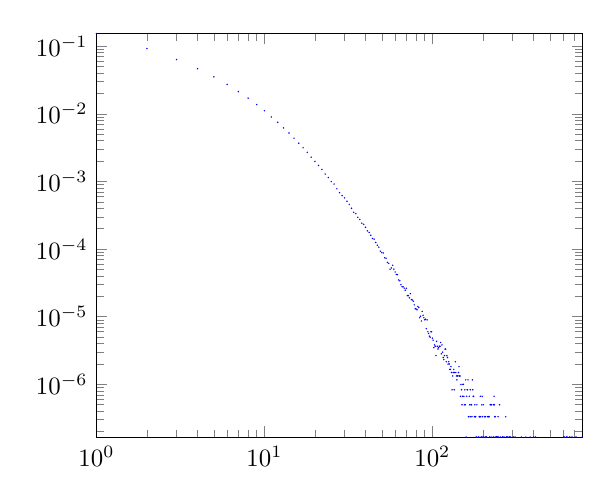
\begin{tikzpicture}
[every mark/.append style={scale=0.1},%
 scale=0.9]
\begin{loglogaxis}[%
  enlargelimits=false%
]
\addplot+[only marks] coordinates
{
  (0, 0.457699779751034)
  (1, 0.153295876313221)
  (2, 0.0918994834048085)
  (3, 0.0632932055701138)
  (4, 0.0463343791678545)
  (5, 0.0350806340902209)
  (6, 0.0271464359673959)
  (7, 0.0212864346861014)
  (8, 0.0169987628035732)
  (9, 0.0136635740915961)
  (10, 0.0110835161671734)
  (11, 0.00896938292436195)
  (12, 0.00748508001008585)
  (13, 0.00617017399790988)
  (14, 0.00519722342170222)
  (15, 0.00436172062656991)
  (16, 0.00366516322756097)
  (17, 0.00314582360923634)
  (18, 0.00269021583128926)
  (19, 0.00228402934992739)
  (20, 0.00197552065003188)
  (21, 0.00172209090356972)
  (22, 0.00150144228649236)
  (23, 0.00128328969449505)
  (24, 0.00113985145322756)
  (25, 0.000993417981864004)
  (26, 0.000914377187662082)
  (27, 0.000779092628322793)
  (28, 0.000681414846856418)
  (29, 0.000616185391430832)
  (30, 0.000570424931629719)
  (31, 0.000509022714660226)
  (32, 0.000458270204699002)
  (33, 0.000401194431201632)
  (34, 0.000349942716224403)
  (35, 0.000333801754040016)
  (36, 0.000294697361119077)
  (37, 0.000273897152118578)
  (38, 0.000241448826077800)
  (39, 0.000232463135789584)
  (40, 0.000210331713413054)
  (41, 0.000185870667628467)
  (42, 0.000176385772324239)
  (43, 0.000160078408467848)
  (44, 0.000143604642939453)
  (45, 0.000140110207827369)
  (46, 0.000124967655675006)
  (47, 0.000114151546994745)
  (48, 0.000106497070082561)
  (49, 0.0000930185346502368)
  (50, 0.0000885256895061286)
  (51, 0.0000876936811461086)
  (52, 0.0000742151457137841)
  (53, 0.0000732167356817601)
  (54, 0.0000633990370335238)
  (55, 0.0000614022169694757)
  (56, 0.0000504197066172118)
  (57, 0.0000525829283532638)
  (58, 0.0000575749785133837)
  (59, 0.0000504197066172118)
  (60, 0.0000457604598010998)
  (61, 0.0000420996230170118)
  (62, 0.0000419332213450078)
  (63, 0.0000349443511208399)
  (64, 0.0000339459410888159)
  (65, 0.0000297858992887159)
  (66, 0.0000277890792246679)
  (67, 0.0000276226775526639)
  (68, 0.0000264578658486360)
  (69, 0.0000246274474565920)
  (70, 0.0000262914641766320)
  (71, 0.0000204674056564920)
  (72, 0.0000204674056564920)
  (73, 0.0000189697906084560)
  (74, 0.0000219650207045280)
  (75, 0.0000179713805764320)
  (76, 0.0000176385772324240)
  (77, 0.0000169729705444080)
  (78, 0.0000149761504803600)
  (79, 0.0000131457320883160)
  (80, 0.0000129793304163120)
  (81, 0.0000126465270723040)
  (82, 0.0000141441421203400)
  (83, 0.0000136449371043280)
  (84, 9.65129697623202e-6)
  (85, 0.0000101505019922440)
  (86, 8.65288694420802e-6)
  (87, 0.0000119809203842880)
  (88, 0.0000104833053362520)
  (89, 9.65129697623202e-6)
  (90, 8.98569028821602e-6)
  (91, 9.15209196022002e-6)
  (92, 6.65606688016002e-6)
  (93, 8.98569028821602e-6)
  (94, 5.99046019214401e-6)
  (95, 5.65765684813601e-6)
  (96, 5.15845183212401e-6)
  (97, 4.99205016012001e-6)
  (98, 5.99046019214401e-6)
  (99, 5.99046019214401e-6)
  (100, 4.82564848811601e-6)
  (101, 4.49284514410801e-6)
  (102, 3.49443511208401e-6)
  (103, 3.82723845609201e-6)
  (104, 3.66083678408801e-6)
  (105, 2.66242675206401e-6)
  (106, 4.32644347210401e-6)
  (107, 3.66083678408801e-6)
  (108, 3.32803344008001e-6)
  (109, 3.49443511208401e-6)
  (110, 3.66083678408801e-6)
  (111, 3.66083678408801e-6)
  (112, 4.16004180010001e-6)
  (113, 2.82882842406801e-6)
  (114, 3.82723845609201e-6)
  (115, 2.99523009607201e-6)
  (116, 2.49602508006000e-6)
  (117, 2.32962340805600e-6)
  (118, 2.66242675206401e-6)
  (119, 3.32803344008001e-6)
  (120, 3.32803344008001e-6)
  (121, 2.16322173605200e-6)
  (122, 2.66242675206401e-6)
  (123, 2.49602508006000e-6)
  (124, 1.99682006404800e-6)
  (125, 2.16322173605200e-6)
  (126, 1.99682006404800e-6)
  (127, 1.66401672004000e-6)
  (128, 1.66401672004000e-6)
  (129, 1.83041839204400e-6)
  (130, 1.49761504803600e-6)
  (131, 8.32008360020001e-7)
  (132, 1.33121337603200e-6)
  (133, 1.49761504803600e-6)
  (134, 1.66401672004000e-6)
  (135, 8.32008360020001e-7)
  (136, 1.49761504803600e-6)
  (137, 2.16322173605200e-6)
  (138, 1.49761504803600e-6)
  (139, 1.33121337603200e-6)
  (140, 1.16481170402800e-6)
  (141, 1.33121337603200e-6)
  (142, 1.33121337603200e-6)
  (143, 1.49761504803600e-6)
  (144, 1.83041839204400e-6)
  (145, 1.33121337603200e-6)
  (146, 1.33121337603200e-6)
  (147, 6.65606688016001e-7)
  (148, 9.98410032024002e-7)
  (149, 8.32008360020001e-7)
  (150, 4.99205016012001e-7)
  (151, 6.65606688016001e-7)
  (152, 9.98410032024002e-7)
  (153, 9.98410032024002e-7)
  (154, 6.65606688016001e-7)
  (155, 4.99205016012001e-7)
  (156, 8.32008360020001e-7)
  (157, 4.99205016012001e-7)
  (158, 1.16481170402800e-6)
  (159, 1.66401672004000e-7)
  (160, 6.65606688016001e-7)
  (161, 8.32008360020001e-7)
  (162, 8.32008360020001e-7)
  (163, 1.16481170402800e-6)
  (164, 3.32803344008001e-7)
  (165, 3.32803344008001e-7)
  (166, 6.65606688016001e-7)
  (167, 4.99205016012001e-7)
  (168, 8.32008360020001e-7)
  (169, 3.32803344008001e-7)
  (170, 4.99205016012001e-7)
  (171, 4.99205016012001e-7)
  (172, 3.32803344008001e-7)
  (173, 1.16481170402800e-6)
  (174, 8.32008360020001e-7)
  (175, 6.65606688016001e-7)
  (176, 6.65606688016001e-7)
  (178, 3.32803344008001e-7)
  (179, 4.99205016012001e-7)
  (180, 3.32803344008001e-7)
  (181, 3.32803344008001e-7)
  (182, 1.66401672004000e-7)
  (183, 1.66401672004000e-7)
  (184, 4.99205016012001e-7)
  (188, 1.66401672004000e-7)
  (189, 1.66401672004000e-7)
  (190, 3.32803344008001e-7)
  (191, 3.32803344008001e-7)
  (192, 3.32803344008001e-7)
  (193, 6.65606688016001e-7)
  (194, 3.32803344008001e-7)
  (195, 1.66401672004000e-7)
  (196, 1.66401672004000e-7)
  (197, 4.99205016012001e-7)
  (198, 6.65606688016001e-7)
  (199, 3.32803344008001e-7)
  (200, 1.66401672004000e-7)
  (201, 4.99205016012001e-7)
  (202, 1.66401672004000e-7)
  (716, 1.66401672004000e-7)
  (205, 3.32803344008001e-7)
  (206, 1.66401672004000e-7)
  (207, 3.32803344008001e-7)
  (208, 1.66401672004000e-7)
  (210, 1.66401672004000e-7)
  (213, 3.32803344008001e-7)
  (215, 3.32803344008001e-7)
  (216, 3.32803344008001e-7)
  (218, 3.32803344008001e-7)
  (219, 1.66401672004000e-7)
  (220, 1.66401672004000e-7)
  (221, 4.99205016012001e-7)
  (223, 4.99205016012001e-7)
  (225, 4.99205016012001e-7)
  (226, 1.66401672004000e-7)
  (231, 4.99205016012001e-7)
  (232, 1.66401672004000e-7)
  (233, 6.65606688016001e-7)
  (234, 4.99205016012001e-7)
  (235, 3.32803344008001e-7)
  (237, 3.32803344008001e-7)
  (239, 1.66401672004000e-7)
  (240, 1.66401672004000e-7)
  (241, 1.66401672004000e-7)
  (242, 1.66401672004000e-7)
  (243, 1.66401672004000e-7)
  (244, 1.66401672004000e-7)
  (246, 3.32803344008001e-7)
  (248, 1.66401672004000e-7)
  (251, 4.99205016012001e-7)
  (605, 1.66401672004000e-7)
  (261, 1.66401672004000e-7)
  (262, 1.66401672004000e-7)
  (267, 1.66401672004000e-7)
  (273, 3.32803344008001e-7)
  (276, 1.66401672004000e-7)
  (278, 1.66401672004000e-7)
  (279, 1.66401672004000e-7)
  (286, 1.66401672004000e-7)
  (287, 1.66401672004000e-7)
  (289, 1.66401672004000e-7)
  (292, 1.66401672004000e-7)
  (305, 1.66401672004000e-7)
  (311, 1.66401672004000e-7)
  (360, 1.66401672004000e-7)
  (339, 1.66401672004000e-7)
  (654, 1.66401672004000e-7)
  (633, 1.66401672004000e-7)
  (779, 1.66401672004000e-7)
  (658, 1.66401672004000e-7)
  (382, 1.66401672004000e-7)
  (401, 1.66401672004000e-7)
  (411, 1.66401672004000e-7)
  (678, 1.66401672004000e-7)
  (630, 1.66401672004000e-7)
  (613, 1.66401672004000e-7)
  (254, 1.66401672004000e-7)
};
\end{loglogaxis}
\end{tikzpicture}

}
%%
%%
\subfigure[Google web graph.]{
  \label{fig:power_law:Google_web_graph}
  %%%%%%%%%%%%%%%%%%%%%%%%%%%%%%%%%%%%%%%%%%%%%%%%%%%%%%%%%%%%%%%%%%%%%%%%%%%
%% This file is part of the book
%%
%% Algorithmic Graph Theory
%% http://code.google.com/p/graph-theory-algorithms-book/
%%
%% Copyright (C) 2009, 2010, 2011 Minh Van Nguyen <nguyenminh2@gmail.com>
%%
%% See the file COPYING for copying conditions.
%%%%%%%%%%%%%%%%%%%%%%%%%%%%%%%%%%%%%%%%%%%%%%%%%%%%%%%%%%%%%%%%%%%%%%%%%%%

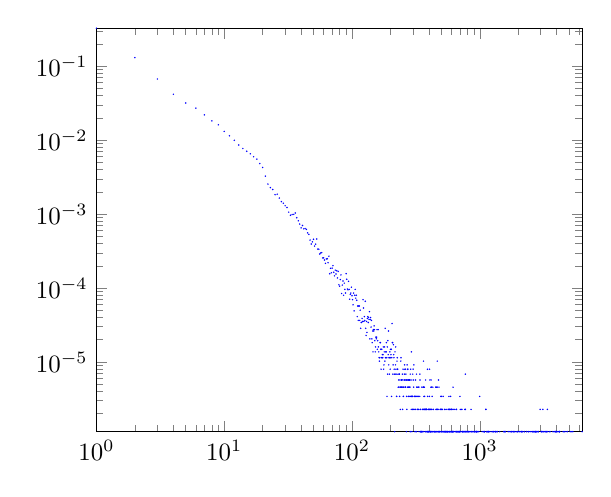
\begin{tikzpicture}
[every mark/.append style={scale=0.1},%
 scale=0.9]
\begin{loglogaxis}[%
  enlargelimits=false%
]
\addplot+[only marks] coordinates
{
  (0, 0.184042032035190)
  (1, 0.327613042173558)
  (2, 0.130798560715397)
  (3, 0.0672172275619041)
  (4, 0.0418321984485554)
  (5, 0.0318243534125955)
  (6, 0.0271230414530843)
  (7, 0.0219877973719742)
  (8, 0.0182559811262398)
  (9, 0.0161628296028521)
  (10, 0.0131584206241106)
  (11, 0.0114615176433391)
  (12, 0.00997929687009454)
  (13, 0.00862382995342174)
  (14, 0.00772855947096894)
  (15, 0.00708793862829544)
  (16, 0.00653867191648447)
  (17, 0.00597227630513678)
  (18, 0.00554747959662601)
  (19, 0.00483034966935514)
  (20, 0.00427537332436527)
  (21, 0.00326476825169876)
  (22, 0.00255106410433551)
  (23, 0.00228499519819849)
  (24, 0.00215253170844787)
  (25, 0.00183165032379333)
  (26, 0.00186134041632364)
  (27, 0.00165122591533986)
  (28, 0.00147651114006531)
  (29, 0.00140571168864686)
  (30, 0.00129837058488340)
  (31, 0.00122985498673652)
  (32, 0.00106427562454821)
  (33, 0.000964928007235231)
  (34, 0.000988908466586639)
  (35, 0.000992334246493984)
  (36, 0.00103458553201790)
  (37, 0.000892986629181008)
  (38, 0.000811909838040535)
  (39, 0.000734258826807406)
  (40, 0.000653182035666932)
  (41, 0.000701142954369747)
  (42, 0.000632627356222869)
  (43, 0.000639478916037557)
  (44, 0.000622350016500837)
  (45, 0.000558402124897084)
  (46, 0.000533279738909895)
  (47, 0.000446493314590513)
  (48, 0.000395106615980352)
  (49, 0.000421370928603323)
  (50, 0.000456770654312545)
  (51, 0.000369984229993161)
  (52, 0.000392822762708789)
  (53, 0.000461338360855671)
  (54, 0.000336868357555502)
  (55, 0.000335726430919720)
  (56, 0.000288907438852684)
  (57, 0.000298042851938935)
  (58, 0.000301468631846280)
  (59, 0.000255791566415025)
  (60, 0.000255791566415025)
  (61, 0.000239804593514086)
  (62, 0.000215824134162677)
  (63, 0.000247798079964555)
  (64, 0.000248940006600337)
  (65, 0.000220391840705803)
  (66, 0.000269494686044401)
  (67, 0.000156443949102046)
  (68, 0.000184992114996580)
  (69, 0.000161011655645172)
  (70, 0.000186134041632362)
  (71, 0.000200979087897519)
  (72, 0.000163295508916734)
  (73, 0.000146166609380014)
  (74, 0.000174714775274548)
  (75, 0.000155302022466265)
  (76, 0.000171288995367204)
  (77, 0.000137031196293763)
  (78, 0.000167863215459860)
  (79, 0.000110766883670792)
  (80, 0.000106199177127666)
  (81, 0.000130179636479075)
  (82, 0.000150734315923139)
  (83, 0.0000845025710478204)
  (84, 0.000109624957035010)
  (85, 0.000124470003300168)
  (86, 0.0000799348645046950)
  (87, 0.000116476516849698)
  (88, 0.0000959218374056339)
  (89, 0.0000856444976836018)
  (90, 0.000156443949102046)
  (91, 0.000131321563114856)
  (92, 0.0000970637640414153)
  (93, 0.0000947799107698526)
  (94, 0.000123328076664386)
  (95, 0.0000959218374056339)
  (96, 0.0000707994514184442)
  (97, 0.0000822187177762577)
  (98, 0.0000856444976836018)
  (99, 0.000102773397220322)
  (100, 0.0000787929378689137)
  (101, 0.0000696575247826628)
  (102, 0.0000593801850606307)
  (103, 0.0000856444976836018)
  (104, 0.0000491028453385984)
  (105, 0.0000799348645046950)
  (106, 0.0000959218374056339)
  (107, 0.0000730833046900069)
  (108, 0.0000799348645046950)
  (109, 0.0000685155981468815)
  (110, 0.0000411093588881289)
  (111, 0.0000570963317890679)
  (112, 0.0000365416523450035)
  (113, 0.0000570963317890679)
  (114, 0.0000570963317890679)
  (115, 0.0000365416523450035)
  (116, 0.0000502447719743798)
  (117, 0.0000285481658945340)
  (118, 0.0000342577990734408)
  (119, 0.0000342577990734408)
  (120, 0.0000388255056165662)
  (121, 0.0000353997257092221)
  (122, 0.0000696575247826628)
  (123, 0.0000536705518817239)
  (124, 0.0000353997257092221)
  (125, 0.0000411093588881289)
  (126, 0.0000365416523450035)
  (127, 0.0000662317448753188)
  (128, 0.0000285481658945340)
  (129, 0.0000228385327156272)
  (130, 0.0000353997257092221)
  (131, 0.0000251223859871899)
  (132, 0.0000388255056165662)
  (133, 0.0000411093588881289)
  (134, 0.0000342577990734408)
  (135, 0.0000399674322523475)
  (136, 0.0000376835789807848)
  (137, 0.0000479609187028171)
  (138, 0.0000205546794440644)
  (139, 0.0000376835789807848)
  (140, 0.0000399674322523475)
  (141, 0.0000296900925303153)
  (142, 0.0000365416523450035)
  (143, 0.0000205546794440644)
  (144, 0.0000182708261725017)
  (145, 0.0000262643126229712)
  (146, 0.0000137031196293763)
  (147, 0.0000274062392587526)
  (148, 0.0000262643126229712)
  (149, 0.0000308320191660967)
  (150, 0.0000274062392587526)
  (151, 0.0000194127528082831)
  (152, 0.0000137031196293763)
  (153, 0.0000159869729009390)
  (154, 0.0000216966060798458)
  (155, 0.0000205546794440644)
  (156, 0.0000216966060798458)
  (157, 0.0000274062392587526)
  (158, 0.0000148450462651576)
  (159, 0.0000194127528082831)
  (160, 0.0000274062392587526)
  (161, 0.0000159869729009390)
  (162, 0.0000137031196293763)
  (163, 0.0000114192663578136)
  (164, 0.0000102773397220322)
  (165, 0.0000114192663578136)
  (166, 0.0000182708261725017)
  (167, 0.0000182708261725017)
  (168, 0.0000148450462651576)
  (169, 7.99348645046950e-6)
  (170, 0.0000114192663578136)
  (171, 0.0000148450462651576)
  (172, 0.0000114192663578136)
  (173, 0.0000125611929935949)
  (174, 0.0000114192663578136)
  (175, 0.0000125611929935949)
  (176, 0.0000159869729009390)
  (177, 7.99348645046950e-6)
  (178, 9.13541308625086e-6)
  (179, 0.0000137031196293763)
  (180, 0.0000159869729009390)
  (181, 0.0000102773397220322)
  (182, 0.0000285481658945340)
  (183, 0.0000114192663578136)
  (184, 0.0000137031196293763)
  (185, 0.0000137031196293763)
  (186, 0.0000182708261725017)
  (187, 0.0000114192663578136)
  (2236, 1.14192663578136e-6)
  (189, 0.0000159869729009390)
  (190, 6.85155981468815e-6)
  (191, 0.0000194127528082831)
  (192, 0.0000125611929935949)
  (193, 0.0000262643126229712)
  (194, 9.13541308625086e-6)
  (195, 0.0000114192663578136)
  (196, 6.85155981468815e-6)
  (197, 0.0000114192663578136)
  (198, 0.0000137031196293763)
  (199, 7.99348645046950e-6)
  (200, 0.0000148450462651576)
  (201, 0.0000114192663578136)
  (202, 0.0000125611929935949)
  (203, 0.0000148450462651576)
  (204, 3.42577990734407e-6)
  (205, 0.0000114192663578136)
  (206, 0.0000331158724376594)
  (207, 0.0000182708261725017)
  (208, 0.0000182708261725017)
  (209, 6.85155981468815e-6)
  (210, 9.13541308625086e-6)
  (211, 0.0000171288995367204)
  (212, 0.0000125611929935949)
  (213, 0.0000114192663578136)
  (214, 7.99348645046950e-6)
  (215, 6.85155981468815e-6)
  (216, 1.14192663578136e-6)
  (217, 0.0000137031196293763)
  (218, 6.85155981468815e-6)
  (219, 9.13541308625086e-6)
  (220, 0.0000159869729009390)
  (221, 7.99348645046950e-6)
  (222, 6.85155981468815e-6)
  (223, 3.42577990734407e-6)
  (224, 3.42577990734407e-6)
  (225, 0.0000102773397220322)
  (226, 0.0000114192663578136)
  (227, 7.99348645046950e-6)
  (228, 7.99348645046950e-6)
  (229, 6.85155981468815e-6)
  (230, 4.56770654312543e-6)
  (232, 5.70963317890679e-6)
  (233, 4.56770654312543e-6)
  (234, 6.85155981468815e-6)
  (235, 6.85155981468815e-6)
  (236, 3.42577990734407e-6)
  (237, 5.70963317890679e-6)
  (238, 4.56770654312543e-6)
  (239, 2.28385327156272e-6)
  (240, 4.56770654312543e-6)
  (241, 0.0000102773397220322)
  (242, 0.0000114192663578136)
  (243, 5.70963317890679e-6)
  (244, 5.70963317890679e-6)
  (245, 4.56770654312543e-6)
  (246, 4.56770654312543e-6)
  (247, 4.56770654312543e-6)
  (248, 6.85155981468815e-6)
  (249, 2.28385327156272e-6)
  (250, 5.70963317890679e-6)
  (251, 7.99348645046950e-6)
  (252, 3.42577990734407e-6)
  (253, 3.42577990734407e-6)
  (254, 4.56770654312543e-6)
  (255, 4.56770654312543e-6)
  (256, 5.70963317890679e-6)
  (257, 6.85155981468815e-6)
  (258, 9.13541308625086e-6)
  (259, 5.70963317890679e-6)
  (260, 7.99348645046950e-6)
  (261, 7.99348645046950e-6)
  (262, 4.56770654312543e-6)
  (263, 4.56770654312543e-6)
  (264, 6.85155981468815e-6)
  (265, 5.70963317890679e-6)
  (266, 5.70963317890679e-6)
  (267, 1.14192663578136e-6)
  (268, 3.42577990734407e-6)
  (269, 2.28385327156272e-6)
  (270, 9.13541308625086e-6)
  (271, 5.70963317890679e-6)
  (272, 7.99348645046950e-6)
  (273, 4.56770654312543e-6)
  (274, 7.99348645046950e-6)
  (275, 4.56770654312543e-6)
  (276, 3.42577990734407e-6)
  (277, 5.70963317890679e-6)
  (278, 4.56770654312543e-6)
  (279, 5.70963317890679e-6)
  (280, 3.42577990734407e-6)
  (281, 5.70963317890679e-6)
  (282, 5.70963317890679e-6)
  (283, 4.56770654312543e-6)
  (284, 4.56770654312543e-6)
  (285, 1.14192663578136e-6)
  (286, 6.85155981468815e-6)
  (287, 3.42577990734407e-6)
  (2336, 1.14192663578136e-6)
  (289, 1.14192663578136e-6)
  (290, 5.70963317890679e-6)
  (291, 2.28385327156272e-6)
  (292, 0.0000137031196293763)
  (293, 3.42577990734407e-6)
  (294, 3.42577990734407e-6)
  (295, 1.14192663578136e-6)
  (296, 3.42577990734407e-6)
  (297, 2.28385327156272e-6)
  (298, 3.42577990734407e-6)
  (299, 6.85155981468815e-6)
  (300, 2.28385327156272e-6)
  (301, 7.99348645046950e-6)
  (302, 5.70963317890679e-6)
  (303, 2.28385327156272e-6)
  (304, 4.56770654312543e-6)
  (305, 9.13541308625086e-6)
  (307, 3.42577990734407e-6)
  (309, 3.42577990734407e-6)
  (310, 2.28385327156272e-6)
  (311, 1.14192663578136e-6)
  (313, 3.42577990734407e-6)
  (314, 5.70963317890679e-6)
  (315, 2.28385327156272e-6)
  (316, 1.14192663578136e-6)
  (317, 3.42577990734407e-6)
  (318, 3.42577990734407e-6)
  (320, 6.85155981468815e-6)
  (321, 1.14192663578136e-6)
  (322, 4.56770654312543e-6)
  (323, 4.56770654312543e-6)
  (325, 2.28385327156272e-6)
  (327, 3.42577990734407e-6)
  (328, 2.28385327156272e-6)
  (329, 3.42577990734407e-6)
  (330, 4.56770654312543e-6)
  (332, 2.28385327156272e-6)
  (333, 3.42577990734407e-6)
  (334, 4.56770654312543e-6)
  (335, 1.14192663578136e-6)
  (339, 3.42577990734407e-6)
  (340, 6.85155981468815e-6)
  (341, 5.70963317890679e-6)
  (342, 2.28385327156272e-6)
  (343, 1.14192663578136e-6)
  (344, 2.28385327156272e-6)
  (345, 1.14192663578136e-6)
  (346, 1.14192663578136e-6)
  (347, 1.14192663578136e-6)
  (349, 1.14192663578136e-6)
  (350, 1.14192663578136e-6)
  (351, 1.14192663578136e-6)
  (352, 4.56770654312543e-6)
  (355, 1.14192663578136e-6)
  (356, 2.28385327156272e-6)
  (358, 2.28385327156272e-6)
  (359, 1.14192663578136e-6)
  (360, 4.56770654312543e-6)
  (361, 1.14192663578136e-6)
  (362, 4.56770654312543e-6)
  (363, 0.0000102773397220322)
  (364, 2.28385327156272e-6)
  (365, 4.56770654312543e-6)
  (366, 3.42577990734407e-6)
  (367, 2.28385327156272e-6)
  (368, 4.56770654312543e-6)
  (370, 3.42577990734407e-6)
  (371, 2.28385327156272e-6)
  (372, 2.28385327156272e-6)
  (373, 1.14192663578136e-6)
  (374, 2.28385327156272e-6)
  (375, 1.14192663578136e-6)
  (376, 2.28385327156272e-6)
  (377, 5.70963317890679e-6)
  (2427, 1.14192663578136e-6)
  (380, 1.14192663578136e-6)
  (381, 2.28385327156272e-6)
  (383, 2.28385327156272e-6)
  (384, 2.28385327156272e-6)
  (385, 2.28385327156272e-6)
  (386, 1.14192663578136e-6)
  (387, 1.14192663578136e-6)
  (4484, 1.14192663578136e-6)
  (389, 1.14192663578136e-6)
  (390, 7.99348645046950e-6)
  (391, 3.42577990734407e-6)
  (392, 1.14192663578136e-6)
  (393, 1.14192663578136e-6)
  (395, 1.14192663578136e-6)
  (396, 2.28385327156272e-6)
  (397, 2.28385327156272e-6)
  (398, 1.14192663578136e-6)
  (399, 1.14192663578136e-6)
  (400, 1.14192663578136e-6)
  (401, 1.14192663578136e-6)
  (402, 1.14192663578136e-6)
  (403, 3.42577990734407e-6)
  (404, 2.28385327156272e-6)
  (405, 7.99348645046950e-6)
  (406, 2.28385327156272e-6)
  (407, 5.70963317890679e-6)
  (408, 2.28385327156272e-6)
  (409, 1.14192663578136e-6)
  (410, 1.14192663578136e-6)
  (411, 2.28385327156272e-6)
  (412, 1.14192663578136e-6)
  (413, 1.14192663578136e-6)
  (414, 1.14192663578136e-6)
  (415, 4.56770654312543e-6)
  (416, 5.70963317890679e-6)
  (417, 2.28385327156272e-6)
  (418, 4.56770654312543e-6)
  (419, 2.28385327156272e-6)
  (420, 1.14192663578136e-6)
  (421, 1.14192663578136e-6)
  (424, 3.42577990734407e-6)
  (425, 1.14192663578136e-6)
  (429, 4.56770654312543e-6)
  (430, 1.14192663578136e-6)
  (431, 2.28385327156272e-6)
  (432, 1.14192663578136e-6)
  (434, 2.28385327156272e-6)
  (440, 1.14192663578136e-6)
  (443, 1.14192663578136e-6)
  (444, 1.14192663578136e-6)
  (445, 1.14192663578136e-6)
  (2496, 1.14192663578136e-6)
  (449, 1.14192663578136e-6)
  (451, 1.14192663578136e-6)
  (453, 4.56770654312543e-6)
  (4550, 1.14192663578136e-6)
  (455, 4.56770654312543e-6)
  (456, 1.14192663578136e-6)
  (457, 4.56770654312543e-6)
  (459, 1.14192663578136e-6)
  (460, 2.28385327156272e-6)
  (463, 1.14192663578136e-6)
  (464, 2.28385327156272e-6)
  (465, 0.0000102773397220322)
  (466, 2.28385327156272e-6)
  (467, 4.56770654312543e-6)
  (470, 1.14192663578136e-6)
  (473, 1.14192663578136e-6)
  (475, 1.14192663578136e-6)
  (476, 5.70963317890679e-6)
  (478, 2.28385327156272e-6)
  (479, 1.14192663578136e-6)
  (480, 4.56770654312543e-6)
  (2128, 1.14192663578136e-6)
  (483, 1.14192663578136e-6)
  (484, 1.14192663578136e-6)
  (489, 1.14192663578136e-6)
  (493, 2.28385327156272e-6)
  (494, 2.28385327156272e-6)
  (495, 3.42577990734407e-6)
  (497, 1.14192663578136e-6)
  (501, 3.42577990734407e-6)
  (502, 1.14192663578136e-6)
  (503, 2.28385327156272e-6)
  (504, 1.14192663578136e-6)
  (505, 2.28385327156272e-6)
  (506, 1.14192663578136e-6)
  (509, 2.28385327156272e-6)
  (514, 1.14192663578136e-6)
  (515, 1.14192663578136e-6)
  (516, 1.14192663578136e-6)
  (517, 3.42577990734407e-6)
  (2569, 1.14192663578136e-6)
  (523, 1.14192663578136e-6)
  (4620, 1.14192663578136e-6)
  (525, 1.14192663578136e-6)
  (526, 1.14192663578136e-6)
  (529, 1.14192663578136e-6)
  (530, 2.28385327156272e-6)
  (534, 1.14192663578136e-6)
  (2137, 1.14192663578136e-6)
  (536, 1.14192663578136e-6)
  (2588, 1.14192663578136e-6)
  (541, 1.14192663578136e-6)
  (543, 1.14192663578136e-6)
  (546, 1.14192663578136e-6)
  (4187, 1.14192663578136e-6)
  (2746, 1.14192663578136e-6)
  (552, 1.14192663578136e-6)
  (553, 2.28385327156272e-6)
  (555, 1.14192663578136e-6)
  (557, 1.14192663578136e-6)
  (560, 1.14192663578136e-6)
  (562, 1.14192663578136e-6)
  (563, 1.14192663578136e-6)
  (565, 1.14192663578136e-6)
  (571, 2.28385327156272e-6)
  (573, 2.28385327156272e-6)
  (574, 3.42577990734407e-6)
  (575, 1.14192663578136e-6)
  (577, 1.14192663578136e-6)
  (2626, 1.14192663578136e-6)
  (579, 1.14192663578136e-6)
  (581, 2.28385327156272e-6)
  (582, 2.28385327156272e-6)
  (585, 1.14192663578136e-6)
  (588, 1.14192663578136e-6)
  (591, 3.42577990734407e-6)
  (594, 2.28385327156272e-6)
  (595, 2.28385327156272e-6)
  (596, 1.14192663578136e-6)
  (597, 1.14192663578136e-6)
  (598, 1.14192663578136e-6)
  (599, 1.14192663578136e-6)
  (600, 2.28385327156272e-6)
  (601, 2.28385327156272e-6)
  (608, 2.28385327156272e-6)
  (609, 1.14192663578136e-6)
  (610, 1.14192663578136e-6)
  (611, 1.14192663578136e-6)
  (612, 1.14192663578136e-6)
  (2661, 1.14192663578136e-6)
  (616, 1.14192663578136e-6)
  (618, 4.56770654312543e-6)
  (619, 1.14192663578136e-6)
  (622, 1.14192663578136e-6)
  (2118, 1.14192663578136e-6)
  (2152, 1.14192663578136e-6)
  (626, 2.28385327156272e-6)
  (627, 1.14192663578136e-6)
  (4731, 1.14192663578136e-6)
  (2685, 1.14192663578136e-6)
  (638, 2.28385327156272e-6)
  (642, 1.14192663578136e-6)
  (643, 1.14192663578136e-6)
  (653, 1.14192663578136e-6)
  (656, 2.28385327156272e-6)
  (657, 2.28385327156272e-6)
  (660, 1.14192663578136e-6)
  (4206, 1.14192663578136e-6)
  (662, 1.14192663578136e-6)
  (663, 1.14192663578136e-6)
  (667, 1.14192663578136e-6)
  (2409, 1.14192663578136e-6)
  (673, 1.14192663578136e-6)
  (676, 1.14192663578136e-6)
  (454, 2.28385327156272e-6)
  (679, 1.14192663578136e-6)
  (2730, 1.14192663578136e-6)
  (687, 1.14192663578136e-6)
  (688, 1.14192663578136e-6)
  (690, 1.14192663578136e-6)
  (695, 1.14192663578136e-6)
  (696, 1.14192663578136e-6)
  (698, 1.14192663578136e-6)
  (2747, 1.14192663578136e-6)
  (700, 3.42577990734407e-6)
  (703, 1.14192663578136e-6)
  (704, 2.28385327156272e-6)
  (711, 1.14192663578136e-6)
  (716, 2.28385327156272e-6)
  (2767, 1.14192663578136e-6)
  (2769, 1.14192663578136e-6)
  (726, 2.28385327156272e-6)
  (727, 1.14192663578136e-6)
  (731, 1.14192663578136e-6)
  (732, 1.14192663578136e-6)
  (735, 1.14192663578136e-6)
  (2736, 1.14192663578136e-6)
  (4219, 1.14192663578136e-6)
  (744, 1.14192663578136e-6)
  (4220, 1.14192663578136e-6)
  (749, 1.14192663578136e-6)
  (4847, 1.14192663578136e-6)
  (758, 1.14192663578136e-6)
  (2810, 1.14192663578136e-6)
  (764, 1.14192663578136e-6)
  (766, 2.28385327156272e-6)
  (767, 2.28385327156272e-6)
  (2176, 1.14192663578136e-6)
  (770, 1.14192663578136e-6)
  (771, 6.85155981468815e-6)
  (772, 2.28385327156272e-6)
  (775, 1.14192663578136e-6)
  (777, 1.14192663578136e-6)
  (784, 1.14192663578136e-6)
  (786, 1.14192663578136e-6)
  (795, 1.14192663578136e-6)
  (800, 1.14192663578136e-6)
  (802, 1.14192663578136e-6)
  (2860, 1.14192663578136e-6)
  (2862, 1.14192663578136e-6)
  (816, 1.14192663578136e-6)
  (818, 1.14192663578136e-6)
  (821, 1.14192663578136e-6)
  (828, 1.14192663578136e-6)
  (2877, 1.14192663578136e-6)
  (481, 1.14192663578136e-6)
  (853, 1.14192663578136e-6)
  (854, 1.14192663578136e-6)
  (855, 2.28385327156272e-6)
  (865, 1.14192663578136e-6)
  (866, 1.14192663578136e-6)
  (881, 1.14192663578136e-6)
  (1171, 1.14192663578136e-6)
  (890, 1.14192663578136e-6)
  (906, 1.14192663578136e-6)
  (911, 1.14192663578136e-6)
  (912, 1.14192663578136e-6)
  (2968, 2.28385327156272e-6)
  (924, 1.14192663578136e-6)
  (937, 1.14192663578136e-6)
  (939, 1.14192663578136e-6)
  (2418, 1.14192663578136e-6)
  (942, 1.14192663578136e-6)
  (947, 1.14192663578136e-6)
  (949, 1.14192663578136e-6)
  (957, 1.14192663578136e-6)
  (970, 1.14192663578136e-6)
  (3022, 1.14192663578136e-6)
  (985, 1.14192663578136e-6)
  (3034, 1.14192663578136e-6)
  (4180, 1.14192663578136e-6)
  (999, 3.42577990734407e-6)
  (3048, 1.14192663578136e-6)
  (5097, 1.14192663578136e-6)
  (1043, 1.14192663578136e-6)
  (2565, 1.14192663578136e-6)
  (3112, 1.14192663578136e-6)
  (3116, 1.14192663578136e-6)
  (3118, 2.28385327156272e-6)
  (1072, 1.14192663578136e-6)
  (1083, 1.14192663578136e-6)
  (1085, 1.14192663578136e-6)
  (1086, 1.14192663578136e-6)
  (1090, 1.14192663578136e-6)
  (6326, 1.14192663578136e-6)
  (3154, 1.14192663578136e-6)
  (1116, 2.28385327156272e-6)
  (1117, 2.28385327156272e-6)
  (1125, 1.14192663578136e-6)
  (188, 3.42577990734407e-6)
  (3181, 1.14192663578136e-6)
  (1136, 1.14192663578136e-6)
  (1144, 1.14192663578136e-6)
  (379, 2.28385327156272e-6)
  (1157, 1.14192663578136e-6)
  (1158, 1.14192663578136e-6)
  (535, 2.28385327156272e-6)
  (1168, 1.14192663578136e-6)
  (2243, 1.14192663578136e-6)
  (1174, 1.14192663578136e-6)
  (5271, 1.14192663578136e-6)
  (540, 1.14192663578136e-6)
  (1197, 1.14192663578136e-6)
  (3247, 1.14192663578136e-6)
  (3249, 1.14192663578136e-6)
  (1225, 1.14192663578136e-6)
  (3296, 1.14192663578136e-6)
  (1258, 1.14192663578136e-6)
  (551, 1.14192663578136e-6)
  (3317, 1.14192663578136e-6)
  (1273, 1.14192663578136e-6)
  (1279, 1.14192663578136e-6)
  (1291, 1.14192663578136e-6)
  (3341, 1.14192663578136e-6)
  (1316, 1.14192663578136e-6)
  (3370, 1.14192663578136e-6)
  (1326, 1.14192663578136e-6)
  (1327, 1.14192663578136e-6)
  (3382, 2.28385327156272e-6)
  (1336, 1.14192663578136e-6)
  (1344, 1.14192663578136e-6)
  (1367, 1.14192663578136e-6)
  (3416, 1.14192663578136e-6)
  (1374, 1.14192663578136e-6)
  (5354, 1.14192663578136e-6)
  (578, 1.14192663578136e-6)
  (1433, 1.14192663578136e-6)
  (3529, 1.14192663578136e-6)
  (3551, 1.14192663578136e-6)
  (1537, 1.14192663578136e-6)
  (2646, 1.14192663578136e-6)
  (941, 1.14192663578136e-6)
  (1558, 1.14192663578136e-6)
  (2097, 1.14192663578136e-6)
  (1569, 1.14192663578136e-6)
  (1577, 1.14192663578136e-6)
  (1588, 1.14192663578136e-6)
  (1667, 1.14192663578136e-6)
  (3728, 1.14192663578136e-6)
  (2329, 1.14192663578136e-6)
  (1699, 1.14192663578136e-6)
  (288, 7.99348645046950e-6)
  (1748, 1.14192663578136e-6)
  (3810, 1.14192663578136e-6)
  (1770, 1.14192663578136e-6)
  (1777, 1.14192663578136e-6)
  (1792, 1.14192663578136e-6)
  (3872, 1.14192663578136e-6)
  (1833, 1.14192663578136e-6)
  (1852, 1.14192663578136e-6)
  (1856, 1.14192663578136e-6)
  (1857, 1.14192663578136e-6)
  (3908, 1.14192663578136e-6)
  (3913, 1.14192663578136e-6)
  (1889, 1.14192663578136e-6)
  (3940, 1.14192663578136e-6)
  (3956, 1.14192663578136e-6)
  (661, 1.14192663578136e-6)
  (2710, 1.14192663578136e-6)
  (3988, 1.14192663578136e-6)
  (1955, 1.14192663578136e-6)
  (4010, 1.14192663578136e-6)
  (1964, 1.14192663578136e-6)
  (1966, 1.14192663578136e-6)
  (4015, 1.14192663578136e-6)
  (1973, 1.14192663578136e-6)
  (2026, 1.14192663578136e-6)
  (5182, 1.14192663578136e-6)
  (4084, 1.14192663578136e-6)
  (2042, 1.14192663578136e-6)
};
\end{loglogaxis}
\end{tikzpicture}

}

\caption{Degree distributions of various real-world networks on
  log-log scales. The horizontal axis represents degree and the
  vertical axis is the corresponding probability of a vertex having
  that degree. The US patent citation network~\cite{LeskovecEtAl2005}
  is a digraph that is not strongly connected and having $3,774,768$
  vertices and $16,518,948$ edges; the corresponding degree
  distribution above considers both the in- and out-degree of
  vertices. The Google web graph~\cite{LeskovecEtAl2008} is a digraph
  on $875,713$ vertices and $5,105,039$ edges; it is not strongly
  connected. The corresponding plot above only shows the degree
  distribution for in-degrees of vertices.}
\label{fig:random_graphs:real_world_scale_free_networks}
\end{figure}

\begin{figure}[!htbp]
\centering
\index{actor collaboration network}
\index{degree distribution}
%%%%%%%%%%%%%%%%%%%%%%%%%%%%%%%%%%%%%%%%%%%%%%%%%%%%%%%%%%%%%%%%%%%%%%%%%%%
%% This file is part of the book
%%
%% Algorithmic Graph Theory
%% http://code.google.com/p/graph-theory-algorithms-book/
%%
%% Copyright (C) 2009--2011 Minh Van Nguyen <nguyenminh2@gmail.com>
%%
%% See the file COPYING for copying conditions.
%%%%%%%%%%%%%%%%%%%%%%%%%%%%%%%%%%%%%%%%%%%%%%%%%%%%%%%%%%%%%%%%%%%%%%%%%%%

\documentclass{article}

\usepackage{pgfplots}
\usetikzlibrary{external}
\tikzexternalize{actor-collaboration-network}

\begin{document}

\begin{figure}
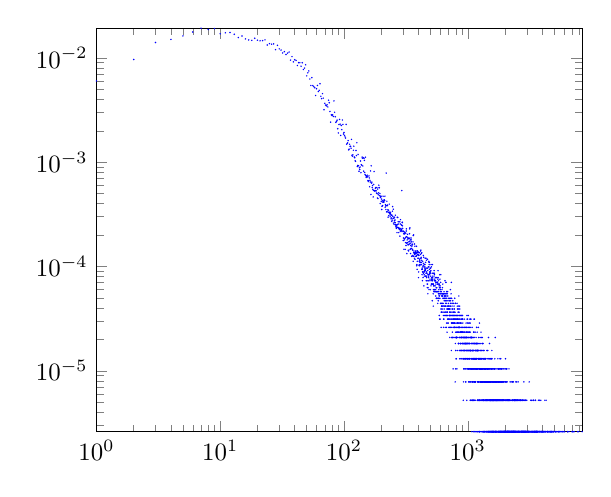
\begin{tikzpicture}
[every mark/.append style={scale=0.1},%
 scale=0.9]
\begin{loglogaxis}[%
  enlargelimits=false%
]
\addplot+[only marks] coordinates
{
  (0, 0.00370399332707742)
  (1, 0.00601084349911400)
  (2, 0.00965227817745881)
  (3, 0.0140392034198742)
  (4, 0.0150453550203331)
  (5, 0.0162470023980833)
  (6, 0.0177327703054967)
  (7, 0.0192758836409155)
  (8, 0.0187311020748639)
  (9, 0.0191012407465353)
  (10, 0.0170055260139733)
  (11, 0.0174173704514668)
  (12, 0.0175346679178415)
  (13, 0.0168517360025042)
  (14, 0.0156605150662095)
  (15, 0.0162157230737167)
  (16, 0.0152043582525300)
  (17, 0.0148681055155891)
  (18, 0.0147325617766671)
  (19, 0.0154363465749156)
  (20, 0.0147899072046726)
  (21, 0.0145839849859258)
  (22, 0.0146465436346590)
  (23, 0.0148837451777724)
  (24, 0.0132963194661675)
  (25, 0.0136925242414777)
  (26, 0.0135387342300086)
  (27, 0.0136117193201974)
  (28, 0.0119956208945898)
  (29, 0.0132103013241594)
  (30, 0.0122015431133366)
  (31, 0.0118913564800345)
  (32, 0.0111588989677833)
  (33, 0.0114769054321770)
  (34, 0.0107705140235647)
  (35, 0.0111197998123250)
  (36, 0.0113700344072578)
  (37, 0.00951934104890076)
  (38, 0.0102856844958824)
  (39, 0.00915702220832100)
  (40, 0.00959753935981726)
  (41, 0.00945938901053145)
  (42, 0.00844802418934478)
  (43, 0.00899541236576024)
  (44, 0.00897716609321306)
  (45, 0.00832812011260615)
  (46, 0.00897195287248530)
  (47, 0.00774163278073243)
  (48, 0.00798665415493745)
  (49, 0.00858878114899447)
  (50, 0.00671984151809023)
  (51, 0.00718642477322532)
  (52, 0.00749661140652741)
  (53, 0.00627150453550232)
  (54, 0.00543738921905970)
  (55, 0.00646178709206579)
  (56, 0.00542696277760417)
  (57, 0.00529402564904612)
  (58, 0.00517672818267138)
  (59, 0.00436085913877595)
  (60, 0.00506203732666052)
  (61, 0.00544520905015135)
  (62, 0.00475185069335842)
  (63, 0.00489000104264423)
  (64, 0.00565113126889812)
  (65, 0.00428787404858722)
  (66, 0.00406631216765715)
  (67, 0.00454332186424777)
  (68, 0.00411583776457093)
  (69, 0.00318267125430087)
  (70, 0.00367010739234694)
  (71, 0.00352935043269727)
  (72, 0.00346679178396409)
  (73, 0.00355280992597222)
  (74, 0.00338859347304760)
  (75, 0.00393076842873522)
  (76, 0.00371181315816907)
  (77, 0.00306537378792614)
  (78, 0.00242154102804710)
  (79, 0.00284641851735999)
  (80, 0.00279949953081010)
  (81, 0.00284902512772388)
  (82, 0.00274476071316857)
  (83, 0.00386820978000203)
  (84, 0.00301063497028461)
  (85, 0.00272390783025750)
  (86, 0.00241111458659157)
  (87, 0.00246846001459699)
  (88, 0.00253101866333018)
  (89, 0.00209050151183400)
  (90, 0.00190543217599832)
  (91, 0.00229381712021685)
  (92, 0.00257011781878842)
  (93, 0.00231467000312791)
  (94, 0.00180638098217078)
  (95, 0.00224429152330308)
  (96, 0.00205140235637575)
  (97, 0.00253883849442183)
  (98, 0.00229903034094462)
  (99, 0.00186372641017620)
  (100, 0.00192889166927326)
  (101, 0.00180898759253466)
  (102, 0.00174642894380147)
  (103, 0.00170472317797935)
  (104, 0.00230163695130850)
  (105, 0.00148576790741320)
  (106, 0.00151183401105203)
  (107, 0.00153008028359920)
  (108, 0.00160827859451569)
  (109, 0.00131112501303305)
  (110, 0.00133197789594412)
  (111, 0.00148576790741320)
  (112, 0.00142060264831613)
  (113, 0.00141799603795225)
  (114, 0.00136325722031071)
  (115, 0.00165519758106558)
  (116, 0.00116776144301950)
  (117, 0.00114169533938067)
  (118, 0.00117558127411115)
  (119, 0.00130069857157752)
  (120, 0.00142320925868001)
  (121, 0.00112084245646961)
  (122, 0.00110259618392243)
  (123, 0.00103221770409760)
  (124, 0.00101918465227819)
  (125, 0.00129287874048587)
  (126, 0.00115733500156397)
  (127, 0.00153529350432697)
  (128, 0.000907100406631224)
  (129, 0.000930559899906170)
  (130, 0.00118600771556668)
  (131, 0.000925346679178404)
  (132, 0.000818475654259207)
  (133, 0.000883640913356279)
  (134, 0.000849754978625801)
  (135, 0.000899280575539576)
  (136, 0.00102700448336983)
  (137, 0.000792409550620379)
  (138, 0.000946199562089467)
  (139, 0.000938379730997819)
  (140, 0.00112084245646961)
  (141, 0.00109216974246690)
  (142, 0.000920133458450639)
  (143, 0.00110520279428632)
  (144, 0.000821082264623090)
  (145, 0.00108956313210302)
  (146, 0.00104003753518925)
  (147, 0.000797622771348144)
  (148, 0.000761130226253784)
  (149, 0.00111562923574185)
  (150, 0.000742883953706604)
  (151, 0.000714211239703893)
  (152, 0.000732457512251073)
  (153, 0.000735064122614956)
  (154, 0.000750703784798253)
  (155, 0.000722031070795541)
  (156, 0.000667292253154001)
  (157, 0.000651652590970704)
  (158, 0.000664685642790119)
  (159, 0.000737670732978839)
  (160, 0.000706391408612244)
  (161, 0.000581274111145867)
  (162, 0.000669898863517884)
  (163, 0.000646439370242939)
  (164, 0.000823688874986973)
  (165, 0.000490042748409967)
  (166, 0.000922740068814521)
  (167, 0.000628193097695759)
  (168, 0.000643832759879056)
  (169, 0.000570847669690336)
  (170, 0.000596913773329164)
  (171, 0.000549994786779273)
  (172, 0.000463976644771139)
  (173, 0.000536961734959859)
  (174, 0.000612553435512461)
  (175, 0.000813262433531441)
  (176, 0.000529141903868210)
  (177, 0.000531748514232093)
  (178, 0.000536961734959859)
  (179, 0.000563027838598687)
  (180, 0.000531748514232093)
  (181, 0.000570847669690336)
  (182, 0.000531748514232093)
  (183, 0.000505682410593264)
  (184, 0.000570847669690336)
  (185, 0.000500469189865499)
  (186, 0.000453550203315608)
  (187, 0.000552601397143156)
  (188, 0.000448336982587842)
  (189, 0.000487436138046084)
  (190, 0.000508289020957147)
  (191, 0.000602126994056930)
  (192, 0.000570847669690336)
  (193, 0.000568241059326453)
  (194, 0.000477009696590553)
  (195, 0.000500469189865499)
  (196, 0.000401417996037952)
  (197, 0.000458763424043373)
  (198, 0.000471796475862787)
  (199, 0.000471796475862787)
  (200, 0.000422270878949014)
  (201, 0.000443123761860077)
  (202, 0.000351892399124179)
  (203, 0.000377958502763007)
  (204, 0.000414451047857366)
  (205, 0.000383171723490772)
  (206, 0.000430090710040663)
  (207, 0.000471796475862787)
  (208, 0.000414451047857366)
  (209, 0.000422270878949014)
  (210, 0.000414451047857366)
  (211, 0.000435303930768428)
  (212, 0.000432697320404545)
  (213, 0.000427484099676780)
  (214, 0.000471796475862787)
  (215, 0.000370138671671358)
  (216, 0.000390991554582421)
  (217, 0.000380565113126889)
  (218, 0.000351892399124179)
  (219, 0.000787196329892613)
  (220, 0.000383171723490772)
  (221, 0.000333646126576999)
  (222, 0.000422270878949014)
  (223, 0.000336252736940882)
  (224, 0.000383171723490772)
  (225, 0.000388384944218538)
  (226, 0.000349285788760296)
  (227, 0.000297153581482640)
  (228, 0.000331039516213116)
  (229, 0.000346679178396413)
  (230, 0.000307580022938171)
  (231, 0.000328432905849233)
  (232, 0.000396204775310186)
  (233, 0.000331039516213116)
  (234, 0.000323219685121468)
  (235, 0.000318006464393702)
  (236, 0.000299760191846522)
  (237, 0.000323219685121468)
  (238, 0.000331039516213116)
  (239, 0.000312793243665936)
  (240, 0.000286727140027108)
  (241, 0.000291940360754874)
  (242, 0.000310186633302054)
  (243, 0.000271087477843812)
  (244, 0.000310186633302054)
  (245, 0.000278907308935460)
  (246, 0.000338859347304764)
  (247, 0.000375351892399124)
  (248, 0.000302366802210405)
  (249, 0.000289333750390991)
  (250, 0.000354499009488061)
  (251, 0.000260661036388280)
  (252, 0.000289333750390991)
  (253, 0.000291940360754874)
  (254, 0.000252841205296632)
  (255, 0.000273694088207694)
  (256, 0.000297153581482640)
  (257, 0.000263267646752163)
  (258, 0.000278907308935460)
  (259, 0.000263267646752163)
  (260, 0.000310186633302054)
  (261, 0.000252841205296632)
  (262, 0.000245021374204984)
  (263, 0.000242414763841101)
  (264, 0.000237201543113335)
  (265, 0.000231988322385570)
  (266, 0.000245021374204984)
  (267, 0.000250234594932749)
  (268, 0.000211135439474507)
  (269, 0.000297153581482640)
  (270, 0.000252841205296632)
  (271, 0.000237201543113335)
  (272, 0.000294546971118757)
  (273, 0.000237201543113335)
  (274, 0.000268480867479929)
  (275, 0.000255447815660515)
  (276, 0.000234594932749452)
  (277, 0.000211135439474507)
  (278, 0.000229381712021687)
  (279, 0.000231988322385570)
  (280, 0.000231988322385570)
  (281, 0.000226775101657804)
  (282, 0.000268480867479929)
  (283, 0.000195495777291210)
  (284, 0.000218955270566156)
  (285, 0.000255447815660515)
  (286, 0.000281513919299343)
  (287, 0.000224168491293921)
  (288, 0.000231988322385570)
  (289, 0.000216348660202273)
  (290, 0.000221561880930038)
  (291, 0.000250234594932749)
  (292, 0.000226775101657804)
  (293, 0.000534355124595976)
  (294, 0.000247627984568866)
  (295, 0.000265874257116046)
  (296, 0.000263267646752163)
  (297, 0.000245021374204984)
  (298, 0.000231988322385570)
  (299, 0.000216348660202273)
  (300, 0.000218955270566156)
  (301, 0.000177249504744031)
  (302, 0.000187675946199562)
  (303, 0.000216348660202273)
  (304, 0.000205922218746742)
  (305, 0.000145970180377437)
  (306, 0.000185069335835679)
  (307, 0.000205922218746742)
  (308, 0.000179856115107913)
  (309, 0.000213742049838390)
  (310, 0.000205922218746742)
  (311, 0.000211135439474507)
  (312, 0.000145970180377437)
  (313, 0.000187675946199562)
  (314, 0.000169429673652382)
  (315, 0.000190282556563445)
  (316, 0.000208528829110624)
  (317, 0.000159003232196851)
  (318, 0.000218955270566156)
  (319, 0.000229381712021687)
  (320, 0.000192889166927327)
  (321, 0.000166823063288499)
  (322, 0.000132937128558023)
  (323, 0.000169429673652382)
  (324, 0.000179856115107913)
  (325, 0.000169429673652382)
  (326, 0.000203315608382859)
  (327, 0.000190282556563445)
  (328, 0.000161609842560734)
  (329, 0.000185069335835679)
  (330, 0.000143363570013554)
  (331, 0.000185069335835679)
  (332, 0.000161609842560734)
  (333, 0.000140756959649671)
  (334, 0.000172036284016265)
  (335, 0.000187675946199562)
  (336, 0.000185069335835679)
  (337, 0.000164216452924617)
  (338, 0.000205922218746742)
  (339, 0.000229381712021687)
  (340, 0.000174642894380148)
  (341, 0.000234594932749452)
  (342, 0.000145970180377437)
  (343, 0.000166823063288499)
  (344, 0.000179856115107913)
  (345, 0.000132937128558023)
  (346, 0.000159003232196851)
  (347, 0.000148576790741320)
  (348, 0.000187675946199562)
  (349, 0.000179856115107913)
  (350, 0.000172036284016265)
  (351, 0.000148576790741320)
  (352, 0.000125117297466375)
  (353, 0.000156396621832968)
  (354, 0.000125117297466375)
  (355, 0.000164216452924617)
  (356, 0.000161609842560734)
  (357, 0.000161609842560734)
  (358, 0.000145970180377437)
  (359, 0.000143363570013554)
  (360, 0.000127723907830257)
  (361, 0.000172036284016265)
  (362, 0.000112084245646961)
  (363, 0.000198102387655093)
  (364, 0.000125117297466375)
  (365, 0.000200708998018976)
  (366, 0.000135543738921906)
  (367, 0.000140756959649671)
  (368, 0.000135543738921906)
  (369, 0.000135543738921906)
  (370, 0.000119904076738609)
  (371, 0.000164216452924617)
  (372, 0.000132937128558023)
  (373, 0.000130330518194140)
  (374, 0.000156396621832968)
  (375, 0.000117297466374726)
  (376, 0.000125117297466375)
  (377, 0.000140756959649671)
  (378, 0.000138150349285789)
  (379, 0.000132937128558023)
  (380, 0.000135543738921906)
  (381, 0.000135543738921906)
  (382, 0.000132937128558023)
  (383, 0.000125117297466375)
  (384, 0.000135543738921906)
  (385, 0.000156396621832968)
  (386, 0.000127723907830257)
  (387, 0.000101657804191429)
  (388, 0.000104264414555312)
  (389, 0.000140756959649671)
  (390, 0.0000938379730997810)
  (391, 0.000112084245646961)
  (392, 0.000140756959649671)
  (393, 0.000135543738921906)
  (394, 0.000130330518194140)
  (395, 0.000119904076738609)
  (396, 0.000130330518194140)
  (397, 0.000138150349285789)
  (398, 0.000119904076738609)
  (399, 0.000127723907830257)
  (400, 0.0000781983109164841)
  (401, 0.0000886247523720154)
  (402, 0.000135543738921906)
  (403, 0.000127723907830257)
  (404, 0.000101657804191429)
  (405, 0.000112084245646961)
  (406, 0.000104264414555312)
  (407, 0.000135543738921906)
  (408, 0.000117297466374726)
  (409, 0.000114690856010843)
  (410, 0.000101657804191429)
  (411, 0.000109477635283078)
  (412, 0.000119904076738609)
  (413, 0.000109477635283078)
  (414, 0.000130330518194140)
  (415, 0.000140756959649671)
  (416, 0.000109477635283078)
  (417, 0.000104264414555312)
  (418, 0.000143363570013554)
  (419, 0.000119904076738609)
  (420, 0.000122510687102492)
  (421, 0.000132937128558023)
  (422, 0.000104264414555312)
  (423, 0.000109477635283078)
  (424, 0.000114690856010843)
  (425, 0.000135543738921906)
  (426, 0.0000938379730997810)
  (427, 0.0000834115316442497)
  (428, 0.0000964445834636638)
  (429, 0.0000938379730997810)
  (430, 0.0000729850901887185)
  (431, 0.0000886247523720154)
  (432, 0.000112084245646961)
  (433, 0.0000886247523720154)
  (434, 0.0000990511938275466)
  (435, 0.0000781983109164841)
  (436, 0.000101657804191429)
  (437, 0.000127723907830257)
  (438, 0.0000860181420081326)
  (439, 0.000106871024919195)
  (440, 0.0000886247523720154)
  (441, 0.000122510687102492)
  (442, 0.0000651652590970701)
  (443, 0.0000990511938275466)
  (444, 0.0000834115316442497)
  (445, 0.0000808049212803669)
  (446, 0.000104264414555312)
  (447, 0.0000912313627358982)
  (448, 0.0000886247523720154)
  (449, 0.0000964445834636638)
  (450, 0.0000990511938275466)
  (451, 0.000104264414555312)
  (452, 0.0000938379730997810)
  (453, 0.000119904076738609)
  (454, 0.0000912313627358982)
  (455, 0.0000938379730997810)
  (456, 0.000109477635283078)
  (457, 0.0000808049212803669)
  (458, 0.0000964445834636638)
  (459, 0.0000808049212803669)
  (460, 0.0000860181420081326)
  (461, 0.000119904076738609)
  (462, 0.0000729850901887185)
  (463, 0.000114690856010843)
  (464, 0.0000886247523720154)
  (465, 0.0000781983109164841)
  (466, 0.0000808049212803669)
  (467, 0.0000964445834636638)
  (468, 0.0000860181420081326)
  (469, 0.0000729850901887185)
  (470, 0.0000677718694609529)
  (471, 0.0000625586487331873)
  (472, 0.000117297466374726)
  (473, 0.0000677718694609529)
  (474, 0.0000964445834636638)
  (475, 0.0000912313627358982)
  (476, 0.0000547388176415389)
  (477, 0.0000834115316442497)
  (478, 0.0000625586487331873)
  (479, 0.0000729850901887185)
  (480, 0.0000990511938275466)
  (481, 0.0000834115316442497)
  (482, 0.0000781983109164841)
  (483, 0.0000808049212803669)
  (484, 0.000112084245646961)
  (485, 0.0000990511938275466)
  (486, 0.0000599520383693045)
  (487, 0.000109477635283078)
  (488, 0.000104264414555312)
  (489, 0.000109477635283078)
  (490, 0.0000938379730997810)
  (491, 0.0000860181420081326)
  (492, 0.0000834115316442497)
  (493, 0.0000886247523720154)
  (494, 0.0000729850901887185)
  (495, 0.0000755917005526013)
  (496, 0.0000886247523720154)
  (497, 0.0000964445834636638)
  (498, 0.0000599520383693045)
  (499, 0.0000886247523720154)
  (500, 0.0000808049212803669)
  (501, 0.0000964445834636638)
  (502, 0.0000860181420081326)
  (503, 0.0000912313627358982)
  (504, 0.0000651652590970701)
  (505, 0.000104264414555312)
  (506, 0.0000729850901887185)
  (507, 0.0000677718694609529)
  (508, 0.0000990511938275466)
  (509, 0.0000755917005526013)
  (510, 0.0000781983109164841)
  (511, 0.0000677718694609529)
  (512, 0.0000677718694609529)
  (513, 0.0000755917005526013)
  (514, 0.0000755917005526013)
  (515, 0.0000677718694609529)
  (516, 0.0000808049212803669)
  (517, 0.0000469189865498905)
  (518, 0.000104264414555312)
  (519, 0.0000729850901887185)
  (520, 0.0000781983109164841)
  (521, 0.0000860181420081326)
  (522, 0.0000755917005526013)
  (523, 0.0000677718694609529)
  (524, 0.0000677718694609529)
  (525, 0.0000547388176415389)
  (526, 0.0000417057658221249)
  (527, 0.0000677718694609529)
  (528, 0.0000599520383693045)
  (529, 0.0000860181420081326)
  (530, 0.0000651652590970701)
  (531, 0.0000599520383693045)
  (532, 0.0000573454280054217)
  (533, 0.0000808049212803669)
  (534, 0.0000912313627358982)
  (535, 0.0000651652590970701)
  (536, 0.0000860181420081326)
  (537, 0.0000729850901887185)
  (538, 0.0000834115316442497)
  (539, 0.0000599520383693045)
  (540, 0.0000599520383693045)
  (541, 0.0000755917005526013)
  (542, 0.0000573454280054217)
  (543, 0.0000573454280054217)
  (544, 0.0000729850901887185)
  (545, 0.0000729850901887185)
  (546, 0.0000651652590970701)
  (547, 0.0000781983109164841)
  (548, 0.0000573454280054217)
  (549, 0.0000729850901887185)
  (550, 0.0000599520383693045)
  (551, 0.0000521322072776561)
  (552, 0.0000703784798248357)
  (553, 0.0000677718694609529)
  (554, 0.0000781983109164841)
  (555, 0.0000625586487331873)
  (556, 0.0000703784798248357)
  (557, 0.0000495255969137733)
  (558, 0.0000495255969137733)
  (559, 0.0000573454280054217)
  (560, 0.0000573454280054217)
  (561, 0.0000625586487331873)
  (562, 0.0000703784798248357)
  (563, 0.0000781983109164841)
  (564, 0.0000781983109164841)
  (565, 0.0000703784798248357)
  (566, 0.0000573454280054217)
  (567, 0.0000495255969137733)
  (568, 0.0000703784798248357)
  (569, 0.0000703784798248357)
  (570, 0.0000573454280054217)
  (571, 0.0000677718694609529)
  (572, 0.0000443123761860077)
  (573, 0.0000755917005526013)
  (574, 0.0000677718694609529)
  (575, 0.0000912313627358982)
  (576, 0.0000781983109164841)
  (577, 0.0000469189865498905)
  (578, 0.0000495255969137733)
  (579, 0.0000573454280054217)
  (580, 0.0000547388176415389)
  (581, 0.0000729850901887185)
  (582, 0.0000677718694609529)
  (583, 0.0000599520383693045)
  (584, 0.0000547388176415389)
  (585, 0.0000495255969137733)
  (586, 0.0000521322072776561)
  (587, 0.0000651652590970701)
  (588, 0.0000338859347304765)
  (589, 0.0000677718694609529)
  (590, 0.0000521322072776561)
  (591, 0.0000625586487331873)
  (592, 0.0000312793243665937)
  (593, 0.0000834115316442497)
  (594, 0.0000547388176415389)
  (595, 0.0000495255969137733)
  (596, 0.0000755917005526013)
  (597, 0.0000651652590970701)
  (598, 0.0000312793243665937)
  (599, 0.0000573454280054217)
  (600, 0.0000625586487331873)
  (601, 0.0000599520383693045)
  (602, 0.0000443123761860077)
  (603, 0.0000547388176415389)
  (604, 0.0000703784798248357)
  (605, 0.0000834115316442497)
  (606, 0.0000443123761860077)
  (607, 0.0000390991554582421)
  (608, 0.0000573454280054217)
  (609, 0.0000260661036388281)
  (610, 0.0000573454280054217)
  (611, 0.0000364925450943593)
  (612, 0.0000364925450943593)
  (613, 0.0000443123761860077)
  (614, 0.0000521322072776561)
  (615, 0.0000417057658221249)
  (616, 0.0000547388176415389)
  (617, 0.0000417057658221249)
  (618, 0.0000390991554582421)
  (619, 0.0000599520383693045)
  (620, 0.0000417057658221249)
  (621, 0.0000364925450943593)
  (622, 0.0000521322072776561)
  (623, 0.0000443123761860077)
  (624, 0.0000625586487331873)
  (625, 0.0000521322072776561)
  (626, 0.0000547388176415389)
  (627, 0.0000547388176415389)
  (628, 0.0000677718694609529)
  (629, 0.0000390991554582421)
  (630, 0.0000495255969137733)
  (631, 0.0000417057658221249)
  (632, 0.0000547388176415389)
  (633, 0.0000443123761860077)
  (634, 0.0000547388176415389)
  (635, 0.0000338859347304765)
  (636, 0.0000495255969137733)
  (637, 0.0000260661036388281)
  (638, 0.0000312793243665937)
  (639, 0.0000547388176415389)
  (640, 0.0000364925450943593)
  (641, 0.0000312793243665937)
  (642, 0.0000417057658221249)
  (643, 0.0000573454280054217)
  (644, 0.0000547388176415389)
  (645, 0.0000469189865498905)
  (646, 0.0000521322072776561)
  (647, 0.0000390991554582421)
  (648, 0.0000495255969137733)
  (649, 0.0000417057658221249)
  (650, 0.0000338859347304765)
  (651, 0.0000521322072776561)
  (652, 0.0000495255969137733)
  (653, 0.0000547388176415389)
  (654, 0.0000364925450943593)
  (655, 0.0000729850901887185)
  (656, 0.0000364925450943593)
  (657, 0.0000260661036388281)
  (658, 0.0000547388176415389)
  (659, 0.0000495255969137733)
  (660, 0.0000521322072776561)
  (661, 0.0000469189865498905)
  (662, 0.0000417057658221249)
  (663, 0.0000443123761860077)
  (664, 0.0000338859347304765)
  (665, 0.0000703784798248357)
  (666, 0.0000417057658221249)
  (667, 0.0000703784798248357)
  (668, 0.0000521322072776561)
  (669, 0.0000364925450943593)
  (670, 0.0000443123761860077)
  (671, 0.0000547388176415389)
  (672, 0.0000260661036388281)
  (673, 0.0000338859347304765)
  (674, 0.0000286727140027109)
  (675, 0.0000573454280054217)
  (676, 0.0000495255969137733)
  (677, 0.0000469189865498905)
  (678, 0.0000573454280054217)
  (679, 0.0000390991554582421)
  (680, 0.0000234594932749453)
  (681, 0.0000364925450943593)
  (682, 0.0000338859347304765)
  (683, 0.0000547388176415389)
  (684, 0.0000364925450943593)
  (685, 0.0000390991554582421)
  (686, 0.0000312793243665937)
  (687, 0.0000573454280054217)
  (688, 0.0000417057658221249)
  (689, 0.0000521322072776561)
  (690, 0.0000286727140027109)
  (691, 0.0000312793243665937)
  (692, 0.0000469189865498905)
  (693, 0.0000417057658221249)
  (694, 0.0000286727140027109)
  (695, 0.0000390991554582421)
  (696, 0.0000417057658221249)
  (697, 0.0000443123761860077)
  (698, 0.0000390991554582421)
  (699, 0.0000390991554582421)
  (700, 0.0000390991554582421)
  (701, 0.0000495255969137733)
  (702, 0.0000260661036388281)
  (703, 0.0000312793243665937)
  (704, 0.0000312793243665937)
  (705, 0.0000417057658221249)
  (706, 0.0000312793243665937)
  (707, 0.0000338859347304765)
  (708, 0.0000390991554582421)
  (709, 0.0000390991554582421)
  (710, 0.0000338859347304765)
  (711, 0.0000495255969137733)
  (712, 0.0000338859347304765)
  (713, 0.0000364925450943593)
  (714, 0.0000260661036388281)
  (715, 0.0000469189865498905)
  (716, 0.0000208528829110625)
  (717, 0.0000469189865498905)
  (718, 0.0000417057658221249)
  (719, 0.0000364925450943593)
  (720, 0.0000390991554582421)
  (721, 0.0000364925450943593)
  (722, 0.0000312793243665937)
  (723, 0.0000417057658221249)
  (724, 0.0000599520383693045)
  (725, 0.0000338859347304765)
  (726, 0.0000443123761860077)
  (727, 0.0000469189865498905)
  (728, 0.0000260661036388281)
  (729, 0.0000260661036388281)
  (730, 0.0000495255969137733)
  (731, 0.0000495255969137733)
  (732, 0.0000443123761860077)
  (733, 0.0000547388176415389)
  (734, 0.0000312793243665937)
  (735, 0.0000338859347304765)
  (736, 0.0000703784798248357)
  (737, 0.0000156396621832968)
  (738, 0.0000286727140027109)
  (739, 0.0000260661036388281)
  (740, 0.0000208528829110625)
  (741, 0.0000495255969137733)
  (742, 0.0000286727140027109)
  (743, 0.0000312793243665937)
  (744, 0.0000364925450943593)
  (745, 0.0000208528829110625)
  (746, 0.0000417057658221249)
  (747, 0.0000208528829110625)
  (748, 0.0000390991554582421)
  (749, 0.0000286727140027109)
  (750, 0.0000390991554582421)
  (751, 0.0000234594932749453)
  (752, 0.0000312793243665937)
  (753, 0.0000286727140027109)
  (754, 0.0000208528829110625)
  (755, 0.0000443123761860077)
  (756, 0.0000338859347304765)
  (757, 0.0000469189865498905)
  (758, 0.0000338859347304765)
  (759, 0.0000208528829110625)
  (760, 0.0000364925450943593)
  (761, 0.0000104264414555312)
  (762, 0.0000260661036388281)
  (763, 0.0000260661036388281)
  (764, 0.0000338859347304765)
  (765, 0.0000286727140027109)
  (766, 0.0000364925450943593)
  (767, 0.0000443123761860077)
  (768, 0.0000286727140027109)
  (769, 0.0000312793243665937)
  (770, 0.0000312793243665937)
  (771, 0.0000312793243665937)
  (772, 0.0000338859347304765)
  (773, 0.0000364925450943593)
  (774, 0.0000417057658221249)
  (775, 0.0000208528829110625)
  (776, 0.0000390991554582421)
  (777, 0.0000364925450943593)
  (778, 0.0000390991554582421)
  (779, 0.0000260661036388281)
  (780, 0.0000286727140027109)
  (781, 0.0000338859347304765)
  (782, 0.0000312793243665937)
  (783, 0.0000286727140027109)
  (784, 0.0000260661036388281)
  (785, 0.0000495255969137733)
  (786, 0.0000260661036388281)
  (787, 0.0000312793243665937)
  (788, 0.0000286727140027109)
  (789, 0.0000364925450943593)
  (790, 0.0000260661036388281)
  (791, 7.81983109164842e-6)
  (792, 0.0000208528829110625)
  (793, 0.0000443123761860077)
  (794, 0.0000182462725471796)
  (795, 0.0000443123761860077)
  (796, 0.0000312793243665937)
  (797, 0.0000104264414555312)
  (798, 0.0000156396621832968)
  (799, 0.0000234594932749453)
  (800, 0.0000338859347304765)
  (801, 0.0000156396621832968)
  (802, 0.0000312793243665937)
  (803, 0.0000208528829110625)
  (804, 0.0000130330518194140)
  (805, 0.0000286727140027109)
  (806, 0.0000338859347304765)
  (807, 0.0000208528829110625)
  (808, 0.0000130330518194140)
  (809, 0.0000312793243665937)
  (810, 0.0000208528829110625)
  (811, 0.0000208528829110625)
  (812, 0.0000260661036388281)
  (813, 0.0000234594932749453)
  (814, 0.0000208528829110625)
  (815, 0.0000208528829110625)
  (816, 0.0000338859347304765)
  (817, 0.0000104264414555312)
  (818, 0.0000312793243665937)
  (819, 0.0000443123761860077)
  (820, 0.0000260661036388281)
  (821, 0.0000234594932749453)
  (822, 0.0000417057658221249)
  (823, 0.0000312793243665937)
  (824, 0.0000286727140027109)
  (825, 0.0000390991554582421)
  (826, 0.0000234594932749453)
  (827, 0.0000312793243665937)
  (828, 0.0000156396621832968)
  (829, 0.0000286727140027109)
  (830, 0.0000338859347304765)
  (831, 0.0000208528829110625)
  (832, 0.0000286727140027109)
  (833, 0.0000364925450943593)
  (834, 0.0000338859347304765)
  (835, 0.0000260661036388281)
  (836, 0.0000312793243665937)
  (837, 0.0000390991554582421)
  (838, 0.0000417057658221249)
  (839, 0.0000286727140027109)
  (840, 0.0000182462725471796)
  (841, 0.0000182462725471796)
  (842, 0.0000234594932749453)
  (843, 0.0000260661036388281)
  (844, 0.0000260661036388281)
  (845, 0.0000182462725471796)
  (846, 0.0000364925450943593)
  (847, 0.0000521322072776561)
  (848, 0.0000234594932749453)
  (849, 0.0000364925450943593)
  (850, 0.0000312793243665937)
  (851, 0.0000312793243665937)
  (852, 0.0000208528829110625)
  (853, 0.0000260661036388281)
  (854, 0.0000286727140027109)
  (855, 0.0000156396621832968)
  (856, 0.0000260661036388281)
  (857, 0.0000208528829110625)
  (858, 0.0000260661036388281)
  (859, 0.0000417057658221249)
  (860, 0.0000130330518194140)
  (861, 0.0000338859347304765)
  (862, 0.0000390991554582421)
  (863, 0.0000338859347304765)
  (864, 0.0000260661036388281)
  (865, 0.0000234594932749453)
  (866, 0.0000156396621832968)
  (867, 0.0000312793243665937)
  (868, 0.0000182462725471796)
  (869, 0.0000234594932749453)
  (870, 0.0000156396621832968)
  (871, 0.0000286727140027109)
  (872, 0.0000234594932749453)
  (873, 0.0000234594932749453)
  (874, 0.0000286727140027109)
  (875, 0.0000182462725471796)
  (876, 0.0000182462725471796)
  (877, 0.0000338859347304765)
  (878, 0.0000208528829110625)
  (879, 0.0000130330518194140)
  (880, 0.0000208528829110625)
  (881, 0.0000234594932749453)
  (882, 0.0000182462725471796)
  (883, 0.0000260661036388281)
  (884, 0.0000286727140027109)
  (885, 0.0000130330518194140)
  (886, 0.0000156396621832968)
  (887, 0.0000312793243665937)
  (888, 0.0000208528829110625)
  (889, 0.0000208528829110625)
  (890, 0.0000338859347304765)
  (891, 0.0000234594932749453)
  (892, 0.0000156396621832968)
  (893, 0.0000208528829110625)
  (894, 0.0000234594932749453)
  (895, 0.0000234594932749453)
  (896, 0.0000234594932749453)
  (897, 0.0000260661036388281)
  (898, 0.0000156396621832968)
  (899, 0.0000312793243665937)
  (900, 0.0000182462725471796)
  (901, 0.0000312793243665937)
  (902, 0.0000234594932749453)
  (903, 0.0000182462725471796)
  (904, 0.0000234594932749453)
  (905, 0.0000312793243665937)
  (906, 0.0000338859347304765)
  (907, 0.0000182462725471796)
  (908, 0.0000260661036388281)
  (909, 0.0000208528829110625)
  (910, 0.0000234594932749453)
  (911, 0.0000286727140027109)
  (912, 0.0000130330518194140)
  (913, 0.0000312793243665937)
  (914, 0.0000156396621832968)
  (915, 0.0000208528829110625)
  (916, 0.0000208528829110625)
  (917, 0.0000182462725471796)
  (918, 0.0000182462725471796)
  (919, 0.0000156396621832968)
  (920, 5.21322072776561e-6)
  (921, 0.0000208528829110625)
  (922, 0.0000182462725471796)
  (923, 7.81983109164842e-6)
  (924, 0.0000130330518194140)
  (925, 0.0000156396621832968)
  (926, 0.0000130330518194140)
  (927, 0.0000208528829110625)
  (928, 0.0000104264414555312)
  (929, 0.0000104264414555312)
  (930, 0.0000234594932749453)
  (931, 0.0000260661036388281)
  (932, 0.0000130330518194140)
  (933, 0.0000208528829110625)
  (934, 0.0000234594932749453)
  (935, 0.0000234594932749453)
  (936, 0.0000260661036388281)
  (937, 0.0000156396621832968)
  (938, 0.0000156396621832968)
  (939, 0.0000130330518194140)
  (940, 0.0000208528829110625)
  (941, 0.0000312793243665937)
  (942, 0.0000182462725471796)
  (943, 0.0000156396621832968)
  (944, 0.0000182462725471796)
  (945, 0.0000208528829110625)
  (946, 0.0000104264414555312)
  (947, 0.0000182462725471796)
  (948, 0.0000260661036388281)
  (949, 0.0000156396621832968)
  (950, 0.0000182462725471796)
  (951, 0.0000208528829110625)
  (952, 0.0000156396621832968)
  (953, 0.0000130330518194140)
  (954, 0.0000130330518194140)
  (955, 0.0000182462725471796)
  (956, 0.0000182462725471796)
  (957, 0.0000182462725471796)
  (958, 0.0000260661036388281)
  (959, 0.0000208528829110625)
  (960, 0.0000182462725471796)
  (961, 0.0000130330518194140)
  (962, 7.81983109164842e-6)
  (963, 7.81983109164842e-6)
  (964, 0.0000104264414555312)
  (965, 0.0000208528829110625)
  (966, 0.0000234594932749453)
  (967, 0.0000208528829110625)
  (968, 0.0000104264414555312)
  (969, 0.0000286727140027109)
  (970, 0.0000182462725471796)
  (971, 0.0000156396621832968)
  (972, 0.0000156396621832968)
  (973, 0.0000208528829110625)
  (974, 0.0000260661036388281)
  (975, 0.0000208528829110625)
  (976, 0.0000234594932749453)
  (977, 0.0000130330518194140)
  (978, 0.0000182462725471796)
  (979, 0.0000234594932749453)
  (980, 0.0000208528829110625)
  (981, 0.0000182462725471796)
  (982, 5.21322072776561e-6)
  (983, 0.0000208528829110625)
  (984, 0.0000260661036388281)
  (985, 0.0000338859347304765)
  (986, 0.0000182462725471796)
  (987, 0.0000156396621832968)
  (988, 0.0000312793243665937)
  (989, 0.0000208528829110625)
  (990, 0.0000104264414555312)
  (991, 0.0000156396621832968)
  (992, 0.0000130330518194140)
  (993, 0.0000130330518194140)
  (994, 0.0000130330518194140)
  (995, 0.0000182462725471796)
  (996, 0.0000312793243665937)
  (997, 0.0000156396621832968)
  (998, 0.0000286727140027109)
  (999, 0.0000182462725471796)
  (1000, 0.0000104264414555312)
  (1001, 0.0000234594932749453)
  (1002, 0.0000130330518194140)
  (1003, 0.0000260661036388281)
  (1004, 0.0000234594932749453)
  (1005, 0.0000234594932749453)
  (1006, 0.0000182462725471796)
  (1007, 0.0000104264414555312)
  (1008, 0.0000286727140027109)
  (1009, 0.0000208528829110625)
  (1010, 0.0000156396621832968)
  (1011, 0.0000338859347304765)
  (1012, 0.0000104264414555312)
  (1013, 0.0000260661036388281)
  (1014, 0.0000156396621832968)
  (1015, 0.0000130330518194140)
  (1016, 0.0000208528829110625)
  (1017, 0.0000104264414555312)
  (1018, 7.81983109164842e-6)
  (1019, 7.81983109164842e-6)
  (1020, 0.0000130330518194140)
  (1021, 0.0000182462725471796)
  (1022, 0.0000182462725471796)
  (1023, 0.0000182462725471796)
  (1024, 0.0000104264414555312)
  (1025, 0.0000182462725471796)
  (1026, 0.0000234594932749453)
  (1027, 0.0000130330518194140)
  (1028, 0.0000182462725471796)
  (1029, 0.0000286727140027109)
  (1030, 0.0000104264414555312)
  (1031, 0.0000130330518194140)
  (1032, 0.0000156396621832968)
  (1033, 7.81983109164842e-6)
  (1034, 0.0000156396621832968)
  (1035, 0.0000234594932749453)
  (1036, 0.0000260661036388281)
  (1037, 0.0000312793243665937)
  (1038, 0.0000130330518194140)
  (1039, 0.0000208528829110625)
  (1040, 0.0000130330518194140)
  (1041, 0.0000182462725471796)
  (1042, 0.0000208528829110625)
  (1043, 0.0000104264414555312)
  (1044, 5.21322072776561e-6)
  (1045, 0.0000286727140027109)
  (1046, 0.0000234594932749453)
  (1047, 0.0000260661036388281)
  (1048, 0.0000156396621832968)
  (1049, 7.81983109164842e-6)
  (1050, 0.0000156396621832968)
  (1051, 0.0000156396621832968)
  (1052, 0.0000104264414555312)
  (1053, 0.0000156396621832968)
  (1054, 0.0000312793243665937)
  (1055, 0.0000104264414555312)
  (1056, 0.0000208528829110625)
  (1057, 5.21322072776561e-6)
  (1058, 0.0000208528829110625)
  (1059, 0.0000208528829110625)
  (1060, 0.0000312793243665937)
  (1061, 7.81983109164842e-6)
  (1062, 5.21322072776561e-6)
  (1063, 0.0000130330518194140)
  (1064, 0.0000208528829110625)
  (1065, 0.0000104264414555312)
  (1066, 0.0000208528829110625)
  (1067, 0.0000182462725471796)
  (1068, 0.0000104264414555312)
  (1069, 0.0000182462725471796)
  (1070, 0.0000156396621832968)
  (1071, 0.0000104264414555312)
  (1072, 0.0000208528829110625)
  (1073, 0.0000208528829110625)
  (1074, 0.0000130330518194140)
  (1075, 0.0000130330518194140)
  (1076, 0.0000208528829110625)
  (1077, 2.60661036388281e-6)
  (1078, 0.0000104264414555312)
  (1079, 0.0000104264414555312)
  (1080, 5.21322072776561e-6)
  (1081, 0.0000130330518194140)
  (1082, 0.0000130330518194140)
  (1083, 0.0000260661036388281)
  (1084, 7.81983109164842e-6)
  (1085, 5.21322072776561e-6)
  (1086, 7.81983109164842e-6)
  (1087, 0.0000182462725471796)
  (1088, 0.0000156396621832968)
  (1089, 0.0000182462725471796)
  (1090, 0.0000156396621832968)
  (1091, 0.0000208528829110625)
  (1092, 7.81983109164842e-6)
  (1093, 0.0000104264414555312)
  (1094, 0.0000130330518194140)
  (1095, 5.21322072776561e-6)
  (1096, 0.0000104264414555312)
  (1097, 0.0000156396621832968)
  (1098, 0.0000130330518194140)
  (1099, 7.81983109164842e-6)
  (1100, 5.21322072776561e-6)
  (1101, 0.0000156396621832968)
  (1102, 0.0000104264414555312)
  (1103, 5.21322072776561e-6)
  (1104, 0.0000104264414555312)
  (1105, 0.0000104264414555312)
  (1106, 5.21322072776561e-6)
  (1107, 7.81983109164842e-6)
  (1108, 0.0000104264414555312)
  (1109, 0.0000130330518194140)
  (1110, 2.60661036388281e-6)
  (1111, 0.0000130330518194140)
  (1112, 0.0000130330518194140)
  (1113, 0.0000130330518194140)
  (1114, 0.0000156396621832968)
  (1115, 0.0000234594932749453)
  (1116, 0.0000208528829110625)
  (1117, 0.0000182462725471796)
  (1118, 0.0000156396621832968)
  (1119, 5.21322072776561e-6)
  (1120, 0.0000234594932749453)
  (1121, 0.0000182462725471796)
  (1122, 0.0000312793243665937)
  (1123, 0.0000182462725471796)
  (1124, 0.0000104264414555312)
  (1125, 0.0000156396621832968)
  (1126, 0.0000208528829110625)
  (1127, 7.81983109164842e-6)
  (1128, 0.0000182462725471796)
  (1129, 0.0000312793243665937)
  (1130, 2.60661036388281e-6)
  (1131, 7.81983109164842e-6)
  (1132, 7.81983109164842e-6)
  (1133, 0.0000104264414555312)
  (1134, 5.21322072776561e-6)
  (1135, 0.0000130330518194140)
  (1136, 0.0000130330518194140)
  (1137, 0.0000130330518194140)
  (1138, 0.0000104264414555312)
  (1139, 0.0000182462725471796)
  (1140, 0.0000130330518194140)
  (1141, 0.0000130330518194140)
  (1142, 0.0000130330518194140)
  (1143, 0.0000104264414555312)
  (1144, 0.0000104264414555312)
  (1145, 0.0000234594932749453)
  (1146, 7.81983109164842e-6)
  (1147, 7.81983109164842e-6)
  (1148, 7.81983109164842e-6)
  (1149, 0.0000130330518194140)
  (1150, 0.0000104264414555312)
  (1151, 0.0000182462725471796)
  (1152, 7.81983109164842e-6)
  (1153, 0.0000182462725471796)
  (1154, 2.60661036388281e-6)
  (1155, 0.0000104264414555312)
  (1156, 0.0000130330518194140)
  (1157, 5.21322072776561e-6)
  (1158, 7.81983109164842e-6)
  (1159, 0.0000156396621832968)
  (1160, 0.0000156396621832968)
  (1161, 0.0000130330518194140)
  (1162, 0.0000156396621832968)
  (1163, 0.0000156396621832968)
  (1164, 0.0000104264414555312)
  (1165, 0.0000130330518194140)
  (1166, 0.0000130330518194140)
  (1167, 0.0000208528829110625)
  (1168, 0.0000104264414555312)
  (1169, 0.0000130330518194140)
  (1170, 0.0000130330518194140)
  (1171, 0.0000104264414555312)
  (1172, 0.0000156396621832968)
  (1173, 0.0000130330518194140)
  (1174, 0.0000182462725471796)
  (1175, 0.0000182462725471796)
  (1177, 0.0000182462725471796)
  (1178, 0.0000260661036388281)
  (1179, 0.0000104264414555312)
  (1180, 0.0000130330518194140)
  (1181, 2.60661036388281e-6)
  (1182, 0.0000260661036388281)
  (1183, 0.0000104264414555312)
  (1184, 0.0000104264414555312)
  (1185, 0.0000156396621832968)
  (1186, 0.0000104264414555312)
  (1187, 0.0000182462725471796)
  (1188, 0.0000156396621832968)
  (1189, 0.0000156396621832968)
  (1190, 0.0000104264414555312)
  (1191, 0.0000234594932749453)
  (1193, 0.0000104264414555312)
  (1194, 2.60661036388281e-6)
  (1195, 5.21322072776561e-6)
  (1196, 0.0000182462725471796)
  (1197, 0.0000156396621832968)
  (1198, 5.21322072776561e-6)
  (1199, 0.0000156396621832968)
  (1200, 7.81983109164842e-6)
  (1201, 7.81983109164842e-6)
  (1202, 5.21322072776561e-6)
  (1203, 0.0000182462725471796)
  (1204, 0.0000104264414555312)
  (1205, 0.0000104264414555312)
  (1206, 0.0000156396621832968)
  (1207, 5.21322072776561e-6)
  (1208, 2.60661036388281e-6)
  (1209, 0.0000130330518194140)
  (1210, 7.81983109164842e-6)
  (1211, 0.0000156396621832968)
  (1212, 0.0000104264414555312)
  (1213, 0.0000130330518194140)
  (1214, 2.60661036388281e-6)
  (1215, 5.21322072776561e-6)
  (1216, 0.0000260661036388281)
  (1217, 0.0000156396621832968)
  (1218, 0.0000156396621832968)
  (1219, 0.0000130330518194140)
  (1221, 0.0000130330518194140)
  (1222, 7.81983109164842e-6)
  (1223, 0.0000130330518194140)
  (1224, 5.21322072776561e-6)
  (1225, 0.0000208528829110625)
  (1226, 7.81983109164842e-6)
  (1227, 7.81983109164842e-6)
  (1228, 0.0000182462725471796)
  (1229, 0.0000130330518194140)
  (1230, 5.21322072776561e-6)
  (1231, 0.0000104264414555312)
  (1232, 2.60661036388281e-6)
  (1233, 7.81983109164842e-6)
  (1234, 0.0000130330518194140)
  (1235, 5.21322072776561e-6)
  (1236, 0.0000182462725471796)
  (1237, 0.0000104264414555312)
  (1238, 2.60661036388281e-6)
  (1239, 0.0000104264414555312)
  (1240, 0.0000130330518194140)
  (1241, 0.0000104264414555312)
  (1242, 0.0000286727140027109)
  (1243, 5.21322072776561e-6)
  (1244, 0.0000130330518194140)
  (1245, 5.21322072776561e-6)
  (1246, 5.21322072776561e-6)
  (1247, 2.60661036388281e-6)
  (1248, 2.60661036388281e-6)
  (1249, 5.21322072776561e-6)
  (1251, 0.0000130330518194140)
  (1252, 0.0000156396621832968)
  (1253, 0.0000104264414555312)
  (1254, 2.60661036388281e-6)
  (1256, 0.0000130330518194140)
  (1257, 0.0000104264414555312)
  (1258, 0.0000208528829110625)
  (1259, 0.0000104264414555312)
  (1260, 7.81983109164842e-6)
  (1261, 5.21322072776561e-6)
  (1262, 0.0000130330518194140)
  (1263, 5.21322072776561e-6)
  (1264, 7.81983109164842e-6)
  (1265, 0.0000104264414555312)
  (1266, 0.0000130330518194140)
  (1267, 0.0000104264414555312)
  (1268, 0.0000156396621832968)
  (1269, 0.0000104264414555312)
  (1270, 7.81983109164842e-6)
  (1271, 0.0000104264414555312)
  (1272, 7.81983109164842e-6)
  (1273, 2.60661036388281e-6)
  (1274, 0.0000182462725471796)
  (1275, 7.81983109164842e-6)
  (1276, 7.81983109164842e-6)
  (1277, 0.0000130330518194140)
  (1278, 0.0000234594932749453)
  (1279, 7.81983109164842e-6)
  (1280, 0.0000104264414555312)
  (1281, 7.81983109164842e-6)
  (1282, 7.81983109164842e-6)
  (1283, 0.0000104264414555312)
  (1284, 0.0000104264414555312)
  (1285, 0.0000208528829110625)
  (1286, 0.0000156396621832968)
  (1287, 0.0000130330518194140)
  (1288, 7.81983109164842e-6)
  (1289, 0.0000130330518194140)
  (1290, 0.0000130330518194140)
  (1291, 7.81983109164842e-6)
  (1292, 0.0000104264414555312)
  (1293, 5.21322072776561e-6)
  (1294, 0.0000104264414555312)
  (1295, 5.21322072776561e-6)
  (1296, 5.21322072776561e-6)
  (1297, 2.60661036388281e-6)
  (1298, 0.0000104264414555312)
  (1299, 0.0000156396621832968)
  (1300, 0.0000104264414555312)
  (1301, 2.60661036388281e-6)
  (1302, 7.81983109164842e-6)
  (1303, 0.0000104264414555312)
  (1304, 0.0000104264414555312)
  (1305, 7.81983109164842e-6)
  (1306, 0.0000104264414555312)
  (1308, 7.81983109164842e-6)
  (1309, 0.0000182462725471796)
  (1310, 2.60661036388281e-6)
  (1311, 0.0000208528829110625)
  (1312, 0.0000130330518194140)
  (1313, 0.0000182462725471796)
  (1314, 7.81983109164842e-6)
  (1315, 7.81983109164842e-6)
  (1316, 7.81983109164842e-6)
  (1317, 5.21322072776561e-6)
  (1318, 5.21322072776561e-6)
  (1319, 2.60661036388281e-6)
  (1320, 7.81983109164842e-6)
  (1321, 7.81983109164842e-6)
  (1322, 5.21322072776561e-6)
  (1323, 0.0000104264414555312)
  (1324, 0.0000156396621832968)
  (1325, 0.0000104264414555312)
  (1326, 5.21322072776561e-6)
  (1327, 7.81983109164842e-6)
  (1328, 0.0000130330518194140)
  (1329, 0.0000182462725471796)
  (1330, 5.21322072776561e-6)
  (1331, 5.21322072776561e-6)
  (1332, 7.81983109164842e-6)
  (1333, 5.21322072776561e-6)
  (1334, 0.0000104264414555312)
  (1335, 0.0000130330518194140)
  (1336, 2.60661036388281e-6)
  (1337, 0.0000130330518194140)
  (1338, 5.21322072776561e-6)
  (1339, 2.60661036388281e-6)
  (1340, 2.60661036388281e-6)
  (1341, 0.0000156396621832968)
  (1342, 5.21322072776561e-6)
  (1343, 5.21322072776561e-6)
  (1344, 2.60661036388281e-6)
  (1345, 5.21322072776561e-6)
  (1346, 7.81983109164842e-6)
  (1347, 7.81983109164842e-6)
  (1348, 5.21322072776561e-6)
  (1349, 0.0000104264414555312)
  (1351, 0.0000130330518194140)
  (1352, 7.81983109164842e-6)
  (1353, 7.81983109164842e-6)
  (1354, 0.0000104264414555312)
  (1355, 0.0000156396621832968)
  (1356, 5.21322072776561e-6)
  (1357, 0.0000104264414555312)
  (1358, 7.81983109164842e-6)
  (1359, 2.60661036388281e-6)
  (1360, 0.0000104264414555312)
  (1361, 2.60661036388281e-6)
  (1362, 7.81983109164842e-6)
  (1363, 0.0000104264414555312)
  (1364, 7.81983109164842e-6)
  (1365, 2.60661036388281e-6)
  (1366, 0.0000130330518194140)
  (1367, 7.81983109164842e-6)
  (1368, 7.81983109164842e-6)
  (1369, 5.21322072776561e-6)
  (1370, 0.0000130330518194140)
  (1371, 5.21322072776561e-6)
  (1372, 2.60661036388281e-6)
  (1373, 7.81983109164842e-6)
  (1374, 2.60661036388281e-6)
  (1376, 0.0000130330518194140)
  (1377, 0.0000104264414555312)
  (1378, 7.81983109164842e-6)
  (1379, 7.81983109164842e-6)
  (1380, 7.81983109164842e-6)
  (1381, 2.60661036388281e-6)
  (1382, 0.0000104264414555312)
  (1383, 7.81983109164842e-6)
  (1384, 7.81983109164842e-6)
  (1385, 2.60661036388281e-6)
  (1386, 0.0000104264414555312)
  (1387, 7.81983109164842e-6)
  (1388, 0.0000104264414555312)
  (1389, 0.0000104264414555312)
  (1390, 5.21322072776561e-6)
  (1391, 0.0000130330518194140)
  (1393, 0.0000104264414555312)
  (1394, 5.21322072776561e-6)
  (1395, 5.21322072776561e-6)
  (1397, 5.21322072776561e-6)
  (1398, 0.0000130330518194140)
  (1399, 0.0000130330518194140)
  (1400, 7.81983109164842e-6)
  (1401, 0.0000104264414555312)
  (1402, 0.0000104264414555312)
  (1403, 7.81983109164842e-6)
  (1404, 5.21322072776561e-6)
  (1405, 5.21322072776561e-6)
  (1406, 2.60661036388281e-6)
  (1407, 0.0000104264414555312)
  (1408, 7.81983109164842e-6)
  (1409, 7.81983109164842e-6)
  (1410, 5.21322072776561e-6)
  (1411, 7.81983109164842e-6)
  (1412, 7.81983109164842e-6)
  (1413, 5.21322072776561e-6)
  (1414, 5.21322072776561e-6)
  (1415, 2.60661036388281e-6)
  (1416, 7.81983109164842e-6)
  (1417, 5.21322072776561e-6)
  (1418, 2.60661036388281e-6)
  (1419, 2.60661036388281e-6)
  (1421, 7.81983109164842e-6)
  (1422, 7.81983109164842e-6)
  (1423, 7.81983109164842e-6)
  (1425, 5.21322072776561e-6)
  (1426, 0.0000156396621832968)
  (1427, 7.81983109164842e-6)
  (1428, 2.60661036388281e-6)
  (1429, 0.0000104264414555312)
  (1430, 0.0000104264414555312)
  (1431, 5.21322072776561e-6)
  (1432, 5.21322072776561e-6)
  (1433, 2.60661036388281e-6)
  (1435, 5.21322072776561e-6)
  (1436, 0.0000104264414555312)
  (1437, 5.21322072776561e-6)
  (1438, 0.0000156396621832968)
  (1439, 2.60661036388281e-6)
  (1440, 7.81983109164842e-6)
  (1441, 0.0000104264414555312)
  (1442, 0.0000104264414555312)
  (1443, 2.60661036388281e-6)
  (1444, 5.21322072776561e-6)
  (1446, 0.0000130330518194140)
  (1447, 7.81983109164842e-6)
  (1448, 7.81983109164842e-6)
  (1449, 7.81983109164842e-6)
  (1450, 0.0000104264414555312)
  (1451, 7.81983109164842e-6)
  (1452, 0.0000156396621832968)
  (1453, 0.0000104264414555312)
  (1454, 0.0000104264414555312)
  (1455, 5.21322072776561e-6)
  (1456, 2.60661036388281e-6)
  (1457, 5.21322072776561e-6)
  (1459, 5.21322072776561e-6)
  (1460, 2.60661036388281e-6)
  (1461, 7.81983109164842e-6)
  (1462, 2.60661036388281e-6)
  (1463, 2.60661036388281e-6)
  (1464, 2.60661036388281e-6)
  (1465, 0.0000104264414555312)
  (1466, 2.60661036388281e-6)
  (1467, 7.81983109164842e-6)
  (1468, 7.81983109164842e-6)
  (1469, 7.81983109164842e-6)
  (1470, 2.60661036388281e-6)
  (1471, 0.0000208528829110625)
  (1472, 0.0000104264414555312)
  (1473, 5.21322072776561e-6)
  (1475, 7.81983109164842e-6)
  (1476, 5.21322072776561e-6)
  (1477, 7.81983109164842e-6)
  (1478, 0.0000130330518194140)
  (1479, 2.60661036388281e-6)
  (1480, 7.81983109164842e-6)
  (1481, 7.81983109164842e-6)
  (1482, 2.60661036388281e-6)
  (1483, 7.81983109164842e-6)
  (1484, 5.21322072776561e-6)
  (1485, 2.60661036388281e-6)
  (1486, 7.81983109164842e-6)
  (1487, 5.21322072776561e-6)
  (1488, 5.21322072776561e-6)
  (1489, 2.60661036388281e-6)
  (1491, 5.21322072776561e-6)
  (1492, 2.60661036388281e-6)
  (1493, 0.0000130330518194140)
  (1494, 5.21322072776561e-6)
  (1495, 0.0000104264414555312)
  (1496, 2.60661036388281e-6)
  (1497, 7.81983109164842e-6)
  (1498, 0.0000182462725471796)
  (1499, 5.21322072776561e-6)
  (1500, 5.21322072776561e-6)
  (1501, 2.60661036388281e-6)
  (1503, 7.81983109164842e-6)
  (1506, 0.0000104264414555312)
  (1507, 2.60661036388281e-6)
  (1508, 2.60661036388281e-6)
  (1509, 7.81983109164842e-6)
  (1510, 0.0000130330518194140)
  (1512, 7.81983109164842e-6)
  (1513, 0.0000104264414555312)
  (1514, 0.0000104264414555312)
  (1515, 5.21322072776561e-6)
  (1516, 7.81983109164842e-6)
  (1517, 5.21322072776561e-6)
  (1518, 5.21322072776561e-6)
  (1519, 5.21322072776561e-6)
  (1520, 5.21322072776561e-6)
  (1521, 2.60661036388281e-6)
  (1522, 7.81983109164842e-6)
  (1523, 2.60661036388281e-6)
  (1524, 2.60661036388281e-6)
  (1525, 5.21322072776561e-6)
  (1526, 7.81983109164842e-6)
  (1527, 0.0000130330518194140)
  (1528, 5.21322072776561e-6)
  (1530, 7.81983109164842e-6)
  (1531, 5.21322072776561e-6)
  (1532, 2.60661036388281e-6)
  (1533, 7.81983109164842e-6)
  (1534, 2.60661036388281e-6)
  (1535, 5.21322072776561e-6)
  (1536, 7.81983109164842e-6)
  (1539, 7.81983109164842e-6)
  (1540, 2.60661036388281e-6)
  (1541, 5.21322072776561e-6)
  (1542, 2.60661036388281e-6)
  (1543, 2.60661036388281e-6)
  (1544, 5.21322072776561e-6)
  (1545, 7.81983109164842e-6)
  (1546, 0.0000130330518194140)
  (1547, 5.21322072776561e-6)
  (1548, 0.0000104264414555312)
  (1549, 2.60661036388281e-6)
  (1550, 2.60661036388281e-6)
  (1551, 2.60661036388281e-6)
  (1552, 0.0000130330518194140)
  (1553, 2.60661036388281e-6)
  (1554, 5.21322072776561e-6)
  (1555, 5.21322072776561e-6)
  (1556, 7.81983109164842e-6)
  (1557, 0.0000104264414555312)
  (1559, 2.60661036388281e-6)
  (1560, 5.21322072776561e-6)
  (1561, 0.0000104264414555312)
  (1562, 0.0000104264414555312)
  (1564, 2.60661036388281e-6)
  (1565, 0.0000104264414555312)
  (1566, 0.0000156396621832968)
  (1567, 5.21322072776561e-6)
  (1568, 5.21322072776561e-6)
  (1569, 0.0000130330518194140)
  (1571, 2.60661036388281e-6)
  (1572, 5.21322072776561e-6)
  (1573, 7.81983109164842e-6)
  (1574, 5.21322072776561e-6)
  (1576, 2.60661036388281e-6)
  (1577, 5.21322072776561e-6)
  (1578, 2.60661036388281e-6)
  (1579, 2.60661036388281e-6)
  (1580, 5.21322072776561e-6)
  (1581, 7.81983109164842e-6)
  (1583, 7.81983109164842e-6)
  (1584, 5.21322072776561e-6)
  (1585, 5.21322072776561e-6)
  (1586, 2.60661036388281e-6)
  (1587, 2.60661036388281e-6)
  (1588, 0.0000104264414555312)
  (1589, 7.81983109164842e-6)
  (1590, 2.60661036388281e-6)
  (1591, 5.21322072776561e-6)
  (1592, 7.81983109164842e-6)
  (1593, 5.21322072776561e-6)
  (1594, 2.60661036388281e-6)
  (1595, 2.60661036388281e-6)
  (1596, 2.60661036388281e-6)
  (1597, 2.60661036388281e-6)
  (1598, 5.21322072776561e-6)
  (1599, 2.60661036388281e-6)
  (1600, 7.81983109164842e-6)
  (1601, 2.60661036388281e-6)
  (1602, 2.60661036388281e-6)
  (1604, 0.0000104264414555312)
  (1605, 5.21322072776561e-6)
  (1606, 5.21322072776561e-6)
  (1607, 2.60661036388281e-6)
  (1608, 5.21322072776561e-6)
  (1609, 5.21322072776561e-6)
  (1610, 7.81983109164842e-6)
  (1611, 2.60661036388281e-6)
  (1612, 5.21322072776561e-6)
  (1613, 7.81983109164842e-6)
  (1616, 7.81983109164842e-6)
  (1617, 2.60661036388281e-6)
  (1618, 2.60661036388281e-6)
  (1620, 5.21322072776561e-6)
  (1621, 5.21322072776561e-6)
  (1622, 5.21322072776561e-6)
  (1623, 2.60661036388281e-6)
  (1624, 2.60661036388281e-6)
  (1626, 2.60661036388281e-6)
  (1627, 7.81983109164842e-6)
  (1628, 2.60661036388281e-6)
  (1629, 0.0000104264414555312)
  (1630, 2.60661036388281e-6)
  (1631, 5.21322072776561e-6)
  (1632, 0.0000104264414555312)
  (1633, 7.81983109164842e-6)
  (1635, 5.21322072776561e-6)
  (1636, 0.0000104264414555312)
  (1637, 5.21322072776561e-6)
  (1639, 5.21322072776561e-6)
  (1640, 5.21322072776561e-6)
  (1642, 7.81983109164842e-6)
  (1644, 2.60661036388281e-6)
  (1646, 2.60661036388281e-6)
  (1647, 0.0000104264414555312)
  (1648, 7.81983109164842e-6)
  (1649, 0.0000104264414555312)
  (1650, 7.81983109164842e-6)
  (1651, 2.60661036388281e-6)
  (1652, 5.21322072776561e-6)
  (1653, 0.0000130330518194140)
  (1655, 2.60661036388281e-6)
  (1656, 5.21322072776561e-6)
  (1658, 5.21322072776561e-6)
  (1659, 2.60661036388281e-6)
  (1660, 2.60661036388281e-6)
  (1661, 0.0000104264414555312)
  (1662, 2.60661036388281e-6)
  (1663, 2.60661036388281e-6)
  (1664, 7.81983109164842e-6)
  (1665, 2.60661036388281e-6)
  (1666, 5.21322072776561e-6)
  (1667, 0.0000208528829110625)
  (1668, 2.60661036388281e-6)
  (1669, 7.81983109164842e-6)
  (1670, 5.21322072776561e-6)
  (1671, 2.60661036388281e-6)
  (1672, 7.81983109164842e-6)
  (1673, 2.60661036388281e-6)
  (1674, 2.60661036388281e-6)
  (1675, 5.21322072776561e-6)
  (1677, 5.21322072776561e-6)
  (1678, 5.21322072776561e-6)
  (1679, 2.60661036388281e-6)
  (1680, 2.60661036388281e-6)
  (1681, 5.21322072776561e-6)
  (1682, 2.60661036388281e-6)
  (1683, 7.81983109164842e-6)
  (1684, 2.60661036388281e-6)
  (1687, 5.21322072776561e-6)
  (1688, 5.21322072776561e-6)
  (1689, 7.81983109164842e-6)
  (1690, 7.81983109164842e-6)
  (1691, 2.60661036388281e-6)
  (1692, 7.81983109164842e-6)
  (1694, 7.81983109164842e-6)
  (1695, 5.21322072776561e-6)
  (1697, 5.21322072776561e-6)
  (1698, 2.60661036388281e-6)
  (1699, 5.21322072776561e-6)
  (1701, 7.81983109164842e-6)
  (1702, 2.60661036388281e-6)
  (1703, 5.21322072776561e-6)
  (1705, 2.60661036388281e-6)
  (1706, 5.21322072776561e-6)
  (1708, 5.21322072776561e-6)
  (1709, 7.81983109164842e-6)
  (1710, 7.81983109164842e-6)
  (1711, 2.60661036388281e-6)
  (1712, 2.60661036388281e-6)
  (1713, 2.60661036388281e-6)
  (1714, 2.60661036388281e-6)
  (1716, 2.60661036388281e-6)
  (1717, 0.0000104264414555312)
  (1718, 5.21322072776561e-6)
  (1719, 2.60661036388281e-6)
  (1721, 5.21322072776561e-6)
  (1723, 5.21322072776561e-6)
  (1724, 2.60661036388281e-6)
  (1725, 5.21322072776561e-6)
  (1727, 7.81983109164842e-6)
  (1729, 5.21322072776561e-6)
  (1731, 5.21322072776561e-6)
  (1732, 2.60661036388281e-6)
  (1733, 5.21322072776561e-6)
  (1734, 2.60661036388281e-6)
  (1735, 5.21322072776561e-6)
  (1736, 5.21322072776561e-6)
  (1740, 2.60661036388281e-6)
  (1742, 5.21322072776561e-6)
  (1745, 7.81983109164842e-6)
  (1750, 0.0000130330518194140)
  (1751, 7.81983109164842e-6)
  (1752, 7.81983109164842e-6)
  (1753, 5.21322072776561e-6)
  (1754, 0.0000104264414555312)
  (1755, 5.21322072776561e-6)
  (1756, 2.60661036388281e-6)
  (1758, 5.21322072776561e-6)
  (1759, 5.21322072776561e-6)
  (1760, 2.60661036388281e-6)
  (1761, 0.0000104264414555312)
  (1763, 2.60661036388281e-6)
  (1764, 0.0000104264414555312)
  (1765, 7.81983109164842e-6)
  (1766, 2.60661036388281e-6)
  (1767, 2.60661036388281e-6)
  (1768, 2.60661036388281e-6)
  (1769, 7.81983109164842e-6)
  (1770, 2.60661036388281e-6)
  (1771, 2.60661036388281e-6)
  (1772, 5.21322072776561e-6)
  (1773, 2.60661036388281e-6)
  (1774, 7.81983109164842e-6)
  (1775, 5.21322072776561e-6)
  (1777, 2.60661036388281e-6)
  (1779, 5.21322072776561e-6)
  (1780, 5.21322072776561e-6)
  (1781, 2.60661036388281e-6)
  (1782, 0.0000104264414555312)
  (1784, 7.81983109164842e-6)
  (1785, 0.0000104264414555312)
  (1786, 7.81983109164842e-6)
  (1788, 0.0000104264414555312)
  (1789, 7.81983109164842e-6)
  (1790, 5.21322072776561e-6)
  (1791, 5.21322072776561e-6)
  (1792, 5.21322072776561e-6)
  (1794, 2.60661036388281e-6)
  (1795, 7.81983109164842e-6)
  (1797, 7.81983109164842e-6)
  (1798, 2.60661036388281e-6)
  (1800, 5.21322072776561e-6)
  (1801, 2.60661036388281e-6)
  (1802, 5.21322072776561e-6)
  (1803, 5.21322072776561e-6)
  (1804, 0.0000104264414555312)
  (1805, 2.60661036388281e-6)
  (1807, 5.21322072776561e-6)
  (1808, 2.60661036388281e-6)
  (1810, 2.60661036388281e-6)
  (1811, 2.60661036388281e-6)
  (1812, 2.60661036388281e-6)
  (1814, 5.21322072776561e-6)
  (1815, 2.60661036388281e-6)
  (1817, 2.60661036388281e-6)
  (1818, 5.21322072776561e-6)
  (1819, 7.81983109164842e-6)
  (1820, 2.60661036388281e-6)
  (1821, 2.60661036388281e-6)
  (1822, 0.0000130330518194140)
  (1823, 5.21322072776561e-6)
  (1824, 5.21322072776561e-6)
  (1825, 2.60661036388281e-6)
  (1826, 5.21322072776561e-6)
  (1828, 2.60661036388281e-6)
  (1829, 0.0000104264414555312)
  (1830, 2.60661036388281e-6)
  (1831, 5.21322072776561e-6)
  (1834, 2.60661036388281e-6)
  (1835, 2.60661036388281e-6)
  (1836, 5.21322072776561e-6)
  (1837, 7.81983109164842e-6)
  (1838, 2.60661036388281e-6)
  (1839, 2.60661036388281e-6)
  (1841, 2.60661036388281e-6)
  (1844, 2.60661036388281e-6)
  (1846, 5.21322072776561e-6)
  (1847, 0.0000130330518194140)
  (1848, 2.60661036388281e-6)
  (1849, 7.81983109164842e-6)
  (1850, 0.0000104264414555312)
  (1851, 2.60661036388281e-6)
  (1852, 2.60661036388281e-6)
  (1853, 7.81983109164842e-6)
  (1854, 2.60661036388281e-6)
  (1856, 2.60661036388281e-6)
  (1857, 0.0000104264414555312)
  (1858, 2.60661036388281e-6)
  (1859, 7.81983109164842e-6)
  (1860, 5.21322072776561e-6)
  (1861, 7.81983109164842e-6)
  (1864, 2.60661036388281e-6)
  (1865, 7.81983109164842e-6)
  (1869, 2.60661036388281e-6)
  (1870, 0.0000104264414555312)
  (1871, 2.60661036388281e-6)
  (1872, 2.60661036388281e-6)
  (1874, 0.0000104264414555312)
  (1875, 2.60661036388281e-6)
  (1877, 5.21322072776561e-6)
  (1879, 5.21322072776561e-6)
  (1880, 2.60661036388281e-6)
  (1881, 2.60661036388281e-6)
  (1882, 5.21322072776561e-6)
  (1883, 5.21322072776561e-6)
  (1884, 2.60661036388281e-6)
  (1886, 2.60661036388281e-6)
  (1888, 7.81983109164842e-6)
  (1889, 2.60661036388281e-6)
  (1890, 5.21322072776561e-6)
  (1891, 5.21322072776561e-6)
  (1892, 2.60661036388281e-6)
  (1893, 2.60661036388281e-6)
  (1894, 7.81983109164842e-6)
  (1898, 0.0000104264414555312)
  (1901, 7.81983109164842e-6)
  (1903, 2.60661036388281e-6)
  (1904, 5.21322072776561e-6)
  (1906, 2.60661036388281e-6)
  (1907, 2.60661036388281e-6)
  (1908, 2.60661036388281e-6)
  (1909, 5.21322072776561e-6)
  (1910, 2.60661036388281e-6)
  (1911, 5.21322072776561e-6)
  (1913, 5.21322072776561e-6)
  (1915, 2.60661036388281e-6)
  (1917, 7.81983109164842e-6)
  (1918, 5.21322072776561e-6)
  (1921, 2.60661036388281e-6)
  (1922, 2.60661036388281e-6)
  (1925, 5.21322072776561e-6)
  (1926, 2.60661036388281e-6)
  (1928, 5.21322072776561e-6)
  (1929, 7.81983109164842e-6)
  (1930, 5.21322072776561e-6)
  (1931, 2.60661036388281e-6)
  (1933, 5.21322072776561e-6)
  (1937, 2.60661036388281e-6)
  (1938, 2.60661036388281e-6)
  (1940, 2.60661036388281e-6)
  (1941, 0.0000104264414555312)
  (1942, 7.81983109164842e-6)
  (1943, 7.81983109164842e-6)
  (1944, 2.60661036388281e-6)
  (1945, 2.60661036388281e-6)
  (1947, 5.21322072776561e-6)
  (1948, 5.21322072776561e-6)
  (1949, 2.60661036388281e-6)
  (1951, 5.21322072776561e-6)
  (1954, 2.60661036388281e-6)
  (1956, 2.60661036388281e-6)
  (1957, 5.21322072776561e-6)
  (1958, 2.60661036388281e-6)
  (1959, 2.60661036388281e-6)
  (1960, 5.21322072776561e-6)
  (1961, 2.60661036388281e-6)
  (1962, 2.60661036388281e-6)
  (1964, 2.60661036388281e-6)
  (1965, 5.21322072776561e-6)
  (1966, 5.21322072776561e-6)
  (1968, 2.60661036388281e-6)
  (1970, 2.60661036388281e-6)
  (1971, 2.60661036388281e-6)
  (1972, 2.60661036388281e-6)
  (1973, 2.60661036388281e-6)
  (1974, 2.60661036388281e-6)
  (1975, 5.21322072776561e-6)
  (1977, 2.60661036388281e-6)
  (1981, 2.60661036388281e-6)
  (1982, 2.60661036388281e-6)
  (1985, 2.60661036388281e-6)
  (1986, 2.60661036388281e-6)
  (1989, 2.60661036388281e-6)
  (1990, 2.60661036388281e-6)
  (1992, 2.60661036388281e-6)
  (1993, 7.81983109164842e-6)
  (1994, 2.60661036388281e-6)
  (1995, 0.0000104264414555312)
  (1996, 2.60661036388281e-6)
  (1998, 2.60661036388281e-6)
  (1999, 5.21322072776561e-6)
  (2001, 2.60661036388281e-6)
  (2002, 7.81983109164842e-6)
  (2004, 5.21322072776561e-6)
  (2007, 2.60661036388281e-6)
  (2008, 2.60661036388281e-6)
  (2010, 2.60661036388281e-6)
  (2011, 2.60661036388281e-6)
  (2012, 5.21322072776561e-6)
  (2014, 5.21322072776561e-6)
  (2015, 0.0000130330518194140)
  (2018, 2.60661036388281e-6)
  (2019, 7.81983109164842e-6)
  (2021, 2.60661036388281e-6)
  (2022, 2.60661036388281e-6)
  (2025, 2.60661036388281e-6)
  (2026, 2.60661036388281e-6)
  (2027, 2.60661036388281e-6)
  (2029, 5.21322072776561e-6)
  (2030, 2.60661036388281e-6)
  (2031, 5.21322072776561e-6)
  (2033, 2.60661036388281e-6)
  (2034, 2.60661036388281e-6)
  (2035, 0.0000104264414555312)
  (2036, 2.60661036388281e-6)
  (2039, 0.0000104264414555312)
  (2041, 7.81983109164842e-6)
  (2044, 5.21322072776561e-6)
  (2046, 2.60661036388281e-6)
  (2047, 0.0000104264414555312)
  (2048, 5.21322072776561e-6)
  (2049, 2.60661036388281e-6)
  (2050, 2.60661036388281e-6)
  (2054, 2.60661036388281e-6)
  (2055, 2.60661036388281e-6)
  (2056, 2.60661036388281e-6)
  (2057, 2.60661036388281e-6)
  (2059, 5.21322072776561e-6)
  (2063, 2.60661036388281e-6)
  (2065, 5.21322072776561e-6)
  (2066, 2.60661036388281e-6)
  (2070, 0.0000104264414555312)
  (2071, 7.81983109164842e-6)
  (2072, 2.60661036388281e-6)
  (2073, 7.81983109164842e-6)
  (2074, 2.60661036388281e-6)
  (2075, 2.60661036388281e-6)
  (2079, 5.21322072776561e-6)
  (2081, 2.60661036388281e-6)
  (2083, 2.60661036388281e-6)
  (2084, 2.60661036388281e-6)
  (2085, 2.60661036388281e-6)
  (2086, 2.60661036388281e-6)
  (2088, 2.60661036388281e-6)
  (2089, 2.60661036388281e-6)
  (2090, 2.60661036388281e-6)
  (2092, 2.60661036388281e-6)
  (2094, 2.60661036388281e-6)
  (2095, 2.60661036388281e-6)
  (2097, 2.60661036388281e-6)
  (2098, 5.21322072776561e-6)
  (2099, 5.21322072776561e-6)
  (2100, 5.21322072776561e-6)
  (2102, 2.60661036388281e-6)
  (2103, 2.60661036388281e-6)
  (2104, 5.21322072776561e-6)
  (2105, 2.60661036388281e-6)
  (2106, 2.60661036388281e-6)
  (2107, 2.60661036388281e-6)
  (2108, 5.21322072776561e-6)
  (2109, 2.60661036388281e-6)
  (2111, 2.60661036388281e-6)
  (2112, 2.60661036388281e-6)
  (2113, 5.21322072776561e-6)
  (2114, 5.21322072776561e-6)
  (2116, 2.60661036388281e-6)
  (2117, 5.21322072776561e-6)
  (2118, 2.60661036388281e-6)
  (2120, 5.21322072776561e-6)
  (2123, 5.21322072776561e-6)
  (2124, 2.60661036388281e-6)
  (2125, 2.60661036388281e-6)
  (2127, 2.60661036388281e-6)
  (2128, 2.60661036388281e-6)
  (2129, 2.60661036388281e-6)
  (2132, 2.60661036388281e-6)
  (2133, 5.21322072776561e-6)
  (2136, 5.21322072776561e-6)
  (2137, 2.60661036388281e-6)
  (2141, 2.60661036388281e-6)
  (2142, 2.60661036388281e-6)
  (2143, 2.60661036388281e-6)
  (2144, 2.60661036388281e-6)
  (2145, 2.60661036388281e-6)
  (2146, 2.60661036388281e-6)
  (2147, 5.21322072776561e-6)
  (2149, 2.60661036388281e-6)
  (2150, 2.60661036388281e-6)
  (2151, 0.0000104264414555312)
  (2155, 5.21322072776561e-6)
  (2156, 2.60661036388281e-6)
  (2160, 2.60661036388281e-6)
  (2161, 5.21322072776561e-6)
  (2163, 2.60661036388281e-6)
  (2165, 2.60661036388281e-6)
  (2168, 5.21322072776561e-6)
  (2169, 5.21322072776561e-6)
  (2170, 2.60661036388281e-6)
  (2171, 2.60661036388281e-6)
  (2173, 2.60661036388281e-6)
  (2174, 5.21322072776561e-6)
  (2175, 2.60661036388281e-6)
  (2177, 5.21322072776561e-6)
  (2178, 2.60661036388281e-6)
  (2180, 2.60661036388281e-6)
  (2182, 2.60661036388281e-6)
  (2183, 2.60661036388281e-6)
  (2186, 2.60661036388281e-6)
  (2187, 2.60661036388281e-6)
  (2188, 5.21322072776561e-6)
  (2189, 2.60661036388281e-6)
  (2195, 2.60661036388281e-6)
  (2198, 7.81983109164842e-6)
  (2199, 5.21322072776561e-6)
  (2200, 2.60661036388281e-6)
  (2211, 2.60661036388281e-6)
  (2212, 2.60661036388281e-6)
  (2213, 2.60661036388281e-6)
  (2215, 2.60661036388281e-6)
  (2216, 2.60661036388281e-6)
  (2217, 5.21322072776561e-6)
  (2223, 2.60661036388281e-6)
  (2225, 2.60661036388281e-6)
  (2226, 2.60661036388281e-6)
  (2227, 2.60661036388281e-6)
  (2228, 2.60661036388281e-6)
  (2231, 2.60661036388281e-6)
  (2235, 2.60661036388281e-6)
  (2237, 2.60661036388281e-6)
  (2239, 2.60661036388281e-6)
  (2241, 7.81983109164842e-6)
  (2242, 2.60661036388281e-6)
  (2244, 2.60661036388281e-6)
  (2245, 2.60661036388281e-6)
  (2246, 2.60661036388281e-6)
  (2251, 5.21322072776561e-6)
  (2254, 2.60661036388281e-6)
  (2255, 2.60661036388281e-6)
  (2256, 2.60661036388281e-6)
  (2258, 2.60661036388281e-6)
  (2260, 2.60661036388281e-6)
  (2261, 2.60661036388281e-6)
  (2264, 2.60661036388281e-6)
  (2266, 2.60661036388281e-6)
  (2267, 2.60661036388281e-6)
  (2269, 2.60661036388281e-6)
  (2272, 5.21322072776561e-6)
  (2273, 2.60661036388281e-6)
  (2275, 2.60661036388281e-6)
  (2279, 2.60661036388281e-6)
  (2283, 2.60661036388281e-6)
  (2286, 2.60661036388281e-6)
  (2290, 7.81983109164842e-6)
  (2292, 2.60661036388281e-6)
  (2293, 2.60661036388281e-6)
  (2297, 2.60661036388281e-6)
  (2299, 2.60661036388281e-6)
  (2300, 2.60661036388281e-6)
  (2301, 5.21322072776561e-6)
  (2302, 7.81983109164842e-6)
  (2303, 5.21322072776561e-6)
  (2304, 2.60661036388281e-6)
  (2305, 2.60661036388281e-6)
  (2306, 2.60661036388281e-6)
  (2307, 2.60661036388281e-6)
  (2309, 5.21322072776561e-6)
  (2310, 2.60661036388281e-6)
  (2311, 5.21322072776561e-6)
  (2312, 5.21322072776561e-6)
  (2314, 5.21322072776561e-6)
  (2315, 2.60661036388281e-6)
  (2316, 2.60661036388281e-6)
  (2319, 5.21322072776561e-6)
  (2324, 2.60661036388281e-6)
  (2325, 2.60661036388281e-6)
  (2326, 2.60661036388281e-6)
  (2330, 2.60661036388281e-6)
  (2333, 7.81983109164842e-6)
  (2336, 2.60661036388281e-6)
  (2337, 2.60661036388281e-6)
  (2338, 2.60661036388281e-6)
  (2340, 5.21322072776561e-6)
  (2344, 2.60661036388281e-6)
  (2345, 2.60661036388281e-6)
  (2347, 2.60661036388281e-6)
  (2348, 2.60661036388281e-6)
  (2349, 2.60661036388281e-6)
  (2351, 2.60661036388281e-6)
  (2352, 2.60661036388281e-6)
  (2354, 2.60661036388281e-6)
  (2355, 2.60661036388281e-6)
  (2356, 2.60661036388281e-6)
  (2357, 2.60661036388281e-6)
  (2358, 2.60661036388281e-6)
  (2362, 5.21322072776561e-6)
  (2363, 2.60661036388281e-6)
  (2365, 5.21322072776561e-6)
  (2367, 2.60661036388281e-6)
  (2371, 5.21322072776561e-6)
  (2372, 2.60661036388281e-6)
  (2376, 2.60661036388281e-6)
  (2377, 2.60661036388281e-6)
  (2381, 2.60661036388281e-6)
  (2384, 5.21322072776561e-6)
  (2386, 2.60661036388281e-6)
  (2387, 2.60661036388281e-6)
  (2390, 2.60661036388281e-6)
  (2391, 2.60661036388281e-6)
  (2392, 2.60661036388281e-6)
  (2393, 5.21322072776561e-6)
  (2395, 2.60661036388281e-6)
  (2396, 5.21322072776561e-6)
  (2398, 5.21322072776561e-6)
  (2399, 2.60661036388281e-6)
  (2400, 2.60661036388281e-6)
  (2403, 5.21322072776561e-6)
  (2405, 5.21322072776561e-6)
  (2406, 5.21322072776561e-6)
  (2407, 2.60661036388281e-6)
  (2408, 2.60661036388281e-6)
  (2410, 5.21322072776561e-6)
  (2412, 5.21322072776561e-6)
  (2413, 2.60661036388281e-6)
  (2414, 5.21322072776561e-6)
  (2420, 5.21322072776561e-6)
  (2421, 2.60661036388281e-6)
  (2425, 2.60661036388281e-6)
  (2426, 5.21322072776561e-6)
  (2429, 2.60661036388281e-6)
  (2431, 2.60661036388281e-6)
  (2432, 2.60661036388281e-6)
  (2433, 2.60661036388281e-6)
  (2435, 2.60661036388281e-6)
  (2438, 2.60661036388281e-6)
  (2439, 2.60661036388281e-6)
  (2440, 2.60661036388281e-6)
  (2442, 2.60661036388281e-6)
  (2444, 7.81983109164842e-6)
  (2445, 2.60661036388281e-6)
  (2450, 2.60661036388281e-6)
  (2453, 2.60661036388281e-6)
  (2454, 2.60661036388281e-6)
  (2458, 5.21322072776561e-6)
  (2461, 2.60661036388281e-6)
  (2462, 5.21322072776561e-6)
  (2468, 2.60661036388281e-6)
  (2472, 5.21322072776561e-6)
  (2473, 2.60661036388281e-6)
  (2474, 2.60661036388281e-6)
  (2476, 7.81983109164842e-6)
  (2482, 5.21322072776561e-6)
  (2484, 2.60661036388281e-6)
  (2486, 2.60661036388281e-6)
  (2487, 2.60661036388281e-6)
  (2488, 2.60661036388281e-6)
  (2495, 2.60661036388281e-6)
  (2499, 2.60661036388281e-6)
  (2501, 5.21322072776561e-6)
  (2502, 5.21322072776561e-6)
  (2509, 2.60661036388281e-6)
  (2511, 2.60661036388281e-6)
  (2513, 2.60661036388281e-6)
  (2514, 5.21322072776561e-6)
  (2515, 5.21322072776561e-6)
  (2516, 2.60661036388281e-6)
  (2517, 2.60661036388281e-6)
  (2519, 2.60661036388281e-6)
  (2523, 5.21322072776561e-6)
  (2526, 5.21322072776561e-6)
  (2531, 2.60661036388281e-6)
  (2535, 2.60661036388281e-6)
  (2537, 5.21322072776561e-6)
  (2541, 2.60661036388281e-6)
  (2542, 2.60661036388281e-6)
  (2543, 2.60661036388281e-6)
  (2544, 2.60661036388281e-6)
  (2546, 2.60661036388281e-6)
  (2550, 7.81983109164842e-6)
  (2551, 2.60661036388281e-6)
  (2557, 2.60661036388281e-6)
  (2561, 2.60661036388281e-6)
  (2562, 5.21322072776561e-6)
  (2565, 2.60661036388281e-6)
  (2573, 2.60661036388281e-6)
  (2574, 2.60661036388281e-6)
  (2579, 2.60661036388281e-6)
  (2581, 2.60661036388281e-6)
  (2583, 2.60661036388281e-6)
  (2584, 5.21322072776561e-6)
  (2585, 2.60661036388281e-6)
  (2586, 2.60661036388281e-6)
  (2587, 2.60661036388281e-6)
  (2589, 5.21322072776561e-6)
  (2590, 2.60661036388281e-6)
  (2593, 2.60661036388281e-6)
  (2594, 2.60661036388281e-6)
  (2595, 5.21322072776561e-6)
  (2597, 2.60661036388281e-6)
  (2602, 5.21322072776561e-6)
  (2606, 2.60661036388281e-6)
  (2607, 2.60661036388281e-6)
  (2608, 2.60661036388281e-6)
  (2612, 2.60661036388281e-6)
  (2613, 2.60661036388281e-6)
  (2614, 2.60661036388281e-6)
  (2633, 2.60661036388281e-6)
  (2635, 5.21322072776561e-6)
  (2640, 2.60661036388281e-6)
  (2641, 2.60661036388281e-6)
  (2642, 2.60661036388281e-6)
  (2645, 5.21322072776561e-6)
  (2650, 5.21322072776561e-6)
  (2652, 5.21322072776561e-6)
  (2655, 5.21322072776561e-6)
  (2656, 2.60661036388281e-6)
  (2661, 2.60661036388281e-6)
  (2670, 2.60661036388281e-6)
  (2676, 2.60661036388281e-6)
  (2677, 5.21322072776561e-6)
  (2683, 2.60661036388281e-6)
  (2684, 5.21322072776561e-6)
  (2693, 2.60661036388281e-6)
  (2698, 2.60661036388281e-6)
  (2702, 2.60661036388281e-6)
  (2704, 2.60661036388281e-6)
  (2705, 2.60661036388281e-6)
  (2706, 2.60661036388281e-6)
  (2710, 2.60661036388281e-6)
  (2711, 2.60661036388281e-6)
  (2712, 5.21322072776561e-6)
  (2714, 2.60661036388281e-6)
  (2716, 2.60661036388281e-6)
  (2717, 2.60661036388281e-6)
  (2719, 2.60661036388281e-6)
  (2723, 2.60661036388281e-6)
  (2734, 2.60661036388281e-6)
  (2735, 5.21322072776561e-6)
  (2736, 2.60661036388281e-6)
  (2738, 2.60661036388281e-6)
  (2744, 2.60661036388281e-6)
  (2749, 2.60661036388281e-6)
  (2750, 5.21322072776561e-6)
  (2752, 2.60661036388281e-6)
  (2754, 2.60661036388281e-6)
  (2757, 2.60661036388281e-6)
  (2761, 2.60661036388281e-6)
  (2766, 2.60661036388281e-6)
  (2768, 5.21322072776561e-6)
  (2773, 2.60661036388281e-6)
  (2774, 2.60661036388281e-6)
  (2775, 2.60661036388281e-6)
  (2778, 2.60661036388281e-6)
  (2782, 2.60661036388281e-6)
  (2784, 2.60661036388281e-6)
  (2786, 5.21322072776561e-6)
  (2791, 5.21322072776561e-6)
  (2794, 2.60661036388281e-6)
  (2795, 5.21322072776561e-6)
  (2798, 2.60661036388281e-6)
  (2799, 5.21322072776561e-6)
  (2805, 2.60661036388281e-6)
  (2806, 2.60661036388281e-6)
  (2811, 2.60661036388281e-6)
  (2812, 2.60661036388281e-6)
  (2821, 2.60661036388281e-6)
  (2822, 2.60661036388281e-6)
  (2823, 2.60661036388281e-6)
  (2826, 2.60661036388281e-6)
  (2831, 2.60661036388281e-6)
  (2833, 2.60661036388281e-6)
  (2836, 2.60661036388281e-6)
  (2837, 7.81983109164842e-6)
  (2838, 2.60661036388281e-6)
  (2843, 2.60661036388281e-6)
  (2849, 2.60661036388281e-6)
  (2850, 2.60661036388281e-6)
  (2851, 2.60661036388281e-6)
  (2853, 5.21322072776561e-6)
  (2856, 2.60661036388281e-6)
  (2858, 2.60661036388281e-6)
  (2861, 2.60661036388281e-6)
  (2863, 2.60661036388281e-6)
  (2868, 2.60661036388281e-6)
  (2869, 2.60661036388281e-6)
  (2871, 2.60661036388281e-6)
  (2872, 2.60661036388281e-6)
  (2878, 5.21322072776561e-6)
  (2881, 2.60661036388281e-6)
  (2884, 2.60661036388281e-6)
  (2885, 2.60661036388281e-6)
  (2887, 2.60661036388281e-6)
  (2892, 2.60661036388281e-6)
  (2903, 5.21322072776561e-6)
  (2905, 2.60661036388281e-6)
  (2909, 2.60661036388281e-6)
  (2910, 2.60661036388281e-6)
  (2914, 2.60661036388281e-6)
  (2915, 2.60661036388281e-6)
  (2917, 2.60661036388281e-6)
  (2919, 2.60661036388281e-6)
  (2923, 5.21322072776561e-6)
  (2924, 2.60661036388281e-6)
  (2926, 2.60661036388281e-6)
  (2930, 2.60661036388281e-6)
  (2938, 2.60661036388281e-6)
  (2939, 2.60661036388281e-6)
  (2941, 2.60661036388281e-6)
  (2947, 2.60661036388281e-6)
  (2948, 2.60661036388281e-6)
  (2949, 2.60661036388281e-6)
  (2955, 2.60661036388281e-6)
  (2956, 5.21322072776561e-6)
  (2961, 2.60661036388281e-6)
  (2966, 2.60661036388281e-6)
  (2973, 2.60661036388281e-6)
  (2977, 2.60661036388281e-6)
  (2978, 2.60661036388281e-6)
  (2984, 2.60661036388281e-6)
  (2993, 2.60661036388281e-6)
  (2998, 2.60661036388281e-6)
  (3000, 5.21322072776561e-6)
  (3001, 2.60661036388281e-6)
  (3016, 2.60661036388281e-6)
  (3023, 2.60661036388281e-6)
  (3025, 2.60661036388281e-6)
  (3031, 2.60661036388281e-6)
  (3037, 2.60661036388281e-6)
  (3040, 2.60661036388281e-6)
  (3049, 2.60661036388281e-6)
  (3063, 2.60661036388281e-6)
  (3065, 2.60661036388281e-6)
  (3072, 2.60661036388281e-6)
  (3075, 2.60661036388281e-6)
  (3076, 2.60661036388281e-6)
  (3077, 2.60661036388281e-6)
  (3081, 2.60661036388281e-6)
  (3089, 2.60661036388281e-6)
  (3090, 2.60661036388281e-6)
  (3092, 2.60661036388281e-6)
  (3102, 2.60661036388281e-6)
  (3104, 2.60661036388281e-6)
  (3108, 2.60661036388281e-6)
  (3109, 2.60661036388281e-6)
  (3120, 2.60661036388281e-6)
  (3122, 2.60661036388281e-6)
  (3126, 2.60661036388281e-6)
  (3135, 7.81983109164842e-6)
  (3152, 2.60661036388281e-6)
  (3159, 2.60661036388281e-6)
  (3167, 2.60661036388281e-6)
  (3172, 2.60661036388281e-6)
  (3174, 2.60661036388281e-6)
  (3178, 2.60661036388281e-6)
  (3182, 2.60661036388281e-6)
  (3185, 2.60661036388281e-6)
  (3208, 2.60661036388281e-6)
  (3209, 2.60661036388281e-6)
  (3219, 5.21322072776561e-6)
  (3236, 2.60661036388281e-6)
  (3242, 2.60661036388281e-6)
  (3246, 2.60661036388281e-6)
  (3263, 2.60661036388281e-6)
  (3266, 2.60661036388281e-6)
  (3269, 2.60661036388281e-6)
  (3272, 2.60661036388281e-6)
  (3290, 5.21322072776561e-6)
  (3291, 2.60661036388281e-6)
  (3292, 5.21322072776561e-6)
  (3294, 2.60661036388281e-6)
  (3315, 2.60661036388281e-6)
  (3321, 2.60661036388281e-6)
  (3327, 2.60661036388281e-6)
  (3328, 2.60661036388281e-6)
  (3332, 2.60661036388281e-6)
  (3344, 2.60661036388281e-6)
  (3350, 2.60661036388281e-6)
  (3357, 2.60661036388281e-6)
  (3361, 2.60661036388281e-6)
  (3364, 2.60661036388281e-6)
  (3365, 2.60661036388281e-6)
  (3371, 2.60661036388281e-6)
  (3387, 2.60661036388281e-6)
  (3389, 5.21322072776561e-6)
  (3396, 2.60661036388281e-6)
  (3397, 5.21322072776561e-6)
  (3414, 2.60661036388281e-6)
  (3422, 2.60661036388281e-6)
  (3424, 2.60661036388281e-6)
  (3429, 2.60661036388281e-6)
  (3434, 2.60661036388281e-6)
  (3438, 2.60661036388281e-6)
  (3444, 2.60661036388281e-6)
  (3450, 2.60661036388281e-6)
  (3454, 2.60661036388281e-6)
  (3457, 2.60661036388281e-6)
  (3461, 2.60661036388281e-6)
  (3468, 2.60661036388281e-6)
  (3471, 2.60661036388281e-6)
  (3472, 2.60661036388281e-6)
  (3481, 2.60661036388281e-6)
  (3494, 2.60661036388281e-6)
  (3503, 5.21322072776561e-6)
  (3504, 2.60661036388281e-6)
  (3508, 2.60661036388281e-6)
  (3523, 5.21322072776561e-6)
  (3524, 2.60661036388281e-6)
  (3525, 2.60661036388281e-6)
  (3526, 2.60661036388281e-6)
  (3530, 2.60661036388281e-6)
  (3533, 2.60661036388281e-6)
  (3554, 2.60661036388281e-6)
  (3557, 2.60661036388281e-6)
  (3558, 2.60661036388281e-6)
  (3564, 2.60661036388281e-6)
  (3567, 2.60661036388281e-6)
  (3579, 2.60661036388281e-6)
  (3581, 2.60661036388281e-6)
  (3586, 2.60661036388281e-6)
  (3587, 2.60661036388281e-6)
  (3593, 2.60661036388281e-6)
  (3597, 2.60661036388281e-6)
  (3598, 2.60661036388281e-6)
  (3600, 2.60661036388281e-6)
  (3603, 2.60661036388281e-6)
  (3604, 2.60661036388281e-6)
  (3619, 2.60661036388281e-6)
  (3633, 2.60661036388281e-6)
  (3636, 2.60661036388281e-6)
  (3639, 2.60661036388281e-6)
  (3641, 2.60661036388281e-6)
  (3642, 2.60661036388281e-6)
  (3649, 2.60661036388281e-6)
  (3652, 2.60661036388281e-6)
  (3655, 2.60661036388281e-6)
  (3664, 2.60661036388281e-6)
  (3688, 2.60661036388281e-6)
  (3690, 2.60661036388281e-6)
  (3703, 2.60661036388281e-6)
  (3717, 5.21322072776561e-6)
  (3718, 2.60661036388281e-6)
  (3719, 2.60661036388281e-6)
  (3755, 2.60661036388281e-6)
  (3777, 5.21322072776561e-6)
  (3778, 2.60661036388281e-6)
  (3786, 2.60661036388281e-6)
  (3806, 2.60661036388281e-6)
  (3807, 2.60661036388281e-6)
  (3817, 2.60661036388281e-6)
  (3823, 2.60661036388281e-6)
  (3858, 2.60661036388281e-6)
  (3864, 2.60661036388281e-6)
  (3892, 5.21322072776561e-6)
  (3896, 2.60661036388281e-6)
  (3910, 2.60661036388281e-6)
  (3912, 2.60661036388281e-6)
  (3936, 2.60661036388281e-6)
  (3952, 2.60661036388281e-6)
  (3954, 2.60661036388281e-6)
  (3958, 2.60661036388281e-6)
  (3970, 2.60661036388281e-6)
  (3982, 2.60661036388281e-6)
  (3985, 2.60661036388281e-6)
  (3996, 2.60661036388281e-6)
  (4013, 2.60661036388281e-6)
  (4014, 2.60661036388281e-6)
  (4026, 2.60661036388281e-6)
  (4029, 2.60661036388281e-6)
  (4053, 2.60661036388281e-6)
  (4057, 2.60661036388281e-6)
  (4080, 2.60661036388281e-6)
  (4081, 2.60661036388281e-6)
  (4090, 2.60661036388281e-6)
  (4112, 2.60661036388281e-6)
  (4135, 2.60661036388281e-6)
  (4181, 2.60661036388281e-6)
  (4189, 2.60661036388281e-6)
  (4195, 5.21322072776561e-6)
  (4197, 2.60661036388281e-6)
  (4216, 2.60661036388281e-6)
  (4218, 2.60661036388281e-6)
  (4248, 2.60661036388281e-6)
  (4250, 2.60661036388281e-6)
  (4288, 2.60661036388281e-6)
  (4292, 2.60661036388281e-6)
  (4293, 5.21322072776561e-6)
  (4375, 2.60661036388281e-6)
  (4391, 2.60661036388281e-6)
  (4410, 2.60661036388281e-6)
  (4413, 2.60661036388281e-6)
  (4417, 2.60661036388281e-6)
  (4426, 2.60661036388281e-6)
  (4436, 2.60661036388281e-6)
  (4452, 2.60661036388281e-6)
  (4505, 2.60661036388281e-6)
  (4513, 2.60661036388281e-6)
  (4525, 2.60661036388281e-6)
  (4585, 2.60661036388281e-6)
  (4597, 2.60661036388281e-6)
  (4609, 2.60661036388281e-6)
  (4620, 2.60661036388281e-6)
  (4622, 2.60661036388281e-6)
  (4657, 2.60661036388281e-6)
  (4664, 2.60661036388281e-6)
  (4670, 2.60661036388281e-6)
  (4711, 2.60661036388281e-6)
  (4713, 2.60661036388281e-6)
  (4734, 2.60661036388281e-6)
  (4750, 2.60661036388281e-6)
  (4756, 2.60661036388281e-6)
  (4763, 2.60661036388281e-6)
  (4801, 2.60661036388281e-6)
  (4836, 2.60661036388281e-6)
  (4852, 2.60661036388281e-6)
  (4890, 2.60661036388281e-6)
  (4912, 2.60661036388281e-6)
  (4931, 2.60661036388281e-6)
  (4941, 2.60661036388281e-6)
  (4981, 2.60661036388281e-6)
  (5068, 2.60661036388281e-6)
  (5109, 2.60661036388281e-6)
  (5115, 2.60661036388281e-6)
  (5132, 2.60661036388281e-6)
  (5185, 2.60661036388281e-6)
  (5240, 2.60661036388281e-6)
  (5351, 2.60661036388281e-6)
  (5362, 2.60661036388281e-6)
  (5406, 2.60661036388281e-6)
  (5440, 2.60661036388281e-6)
  (5446, 2.60661036388281e-6)
  (5469, 2.60661036388281e-6)
  (5490, 2.60661036388281e-6)
  (5622, 2.60661036388281e-6)
  (5738, 2.60661036388281e-6)
  (5803, 2.60661036388281e-6)
  (5849, 2.60661036388281e-6)
  (5881, 2.60661036388281e-6)
  (8382, 2.60661036388281e-6)
  (5994, 2.60661036388281e-6)
  (6004, 2.60661036388281e-6)
  (6080, 2.60661036388281e-6)
  (6381, 2.60661036388281e-6)
  (6399, 2.60661036388281e-6)
  (6445, 2.60661036388281e-6)
  (6566, 2.60661036388281e-6)
  (6951, 2.60661036388281e-6)
  (6978, 2.60661036388281e-6)
  (7013, 2.60661036388281e-6)
  (7175, 2.60661036388281e-6)
  (7230, 2.60661036388281e-6)
  (7706, 2.60661036388281e-6)
  (7868, 2.60661036388281e-6)
};
\end{loglogaxis}
\end{tikzpicture}
\end{figure}

\end{document}

\caption{Degree distribution of an actor collaboration
  network~\cite{BarabasiAlbert1999} on a log-log scale. The horizontal
  axis represents degree and the vertical axis is the corresponding
  probability of a vertex having that degree. The network is an
  undirected, disconnected graph on $383,640$ vertices and
  $16,557,920$ edges.}
\label{fig:random_graphs:actor_collaboration_network}
\end{figure}

But how do we get the whole process started in the first place? The
original description of the
Barab\'asi-Albert\index{Barab\'asi-Albert model} model as contained
in~\cite{BarabasiAlbert1999} is rather ambiguous with respect to
certain details. First, the whole process is supposed to begin with a
small number of vertices. But as the degree of each of these vertices
is zero, it is unclear how the network is to grow via preferential
attachment from the initial pool of vertices. Second, Barab\'asi and
Albert neglected to clearly specify how to select the neighbors for
the newly added vertex. The above ambiguities are resolved in
Bollobas~et~al.~\cite{BollobasEtAl2001}, wherein is given a precise
statement of a random graph process that realizes the
Barab\'asi-Albert model. Fix a sequence of vertices
$v_1, v_2, \dots$ and consider the case where each newly added vertex
is to be connected to $m = 1$ vertex already in a graph. Inductively
define a random graph process $(G_1^t)_{t \geq 0}$ as follows, where
$G_1^t$ is a digraph on $\{v_i \mid 1 \leq i \leq t\}$. Start with the
null\index{null graph} graph $G_1^0$ or the graph $G_1^1$ with one
vertex and one self-loop. Denote by $\deg_G(v)$ the total~(in and out)
degree of vertex $v$ in the graph $G$. For $t > 1$ construct $G_1^t$
from $G_1^{t-1}$ by adding the vertex $v_t$ and a directed edge from
$v_t$ to $v_i$, where $i$ is randomly chosen with probability
\[
\Pr[i = s]
=
\begin{cases}
\deg_{G_1^{t-1}}(v_s) / (2t - 1), & \text{if $1 \leq s \leq t - 1$}, \\[4pt]
1 / (2t - 1), & \text{if $s = t$}.
\end{cases}
\]
The latter process generates a forest. For $m > 1$ the graph evolves
as per the case $m = 1$; i.e. we add $m$ edges from $v_t$ one at a
time. This process can result in self-loops and multiple edges.

Now consider the problem of translating the above procedure into
pseudocode. Fix a positive integer $n > 1$ for the number of vertices
in the scale-free graph to be generated via preferential
attachment. Let $m \geq 1$ be the number of vertices that each newly
added vertex is to be connected to; this is equivalent to the minimum
degree that any new vertex will end up possessing. At any time step,
let $M$ be the contiguous edge list of all edges created thus far in
the above random graph process. It is clear that the frequency~(or
number of occurrences) of a vertex is equivalent to the vertex's
degree. We can thus use $M$ as a pool to sample in constant time from
the degree-skewed distribution. Batagelj and
Brandes~\cite{BatageljBrandes2005} used the latter observation to
construct an algorithm for generating scale-free networks via
preferential attachment; pseudocode is presented in
Algorithm~\ref{alg:random_graphs:scale_free_network_preferential_attachment}.
Note that the algorithm has linear runtime $O(n + m)$, where $n$ is
the order and $m$ the size of the graph generated by the algorithm.

\begin{algorithm}[!htbp]
\index{algorithm!random}
\index{preferential attachment}
\index{scale-free network}
%%%%%%%%%%%%%%%%%%%%%%%%%%%%%%%%%%%%%%%%%%%%%%%%%%%%%%%%%%%%%%%%%%%%%%%%%%%
%% This file is part of the book
%%
%% Algorithmic Graph Theory
%% http://code.google.com/p/graph-theory-algorithms-book/
%%
%% Copyright (C) 2009, 2010, 2011 Minh Van Nguyen <nguyenminh2@gmail.com>
%%
%% See the file COPYING for copying conditions.
%%%%%%%%%%%%%%%%%%%%%%%%%%%%%%%%%%%%%%%%%%%%%%%%%%%%%%%%%%%%%%%%%%%%%%%%%%%

\DontPrintSemicolon
\SetAlgoNoLine
%%
%% input
\KwIn{Positive integer $n > 1$ and minimum degree $d \geq 1$.}
%%
%% output
\KwOut{Scale-free network on $n$ vertices.}
\BlankLine
%%
%% algorithm body
$G \assign \overline{K_n}$\tcc*[f]{vertex set is $V = \{0, 1, \dots, n-1\}$}\;
$M \assign$ list of length $2nd$\;
\For{$v = 0, 1, \dots, n-1$}{
  \For{$i = 0, 1, \dots, d-1$}{
    $M[2(vd + i)] \assign v$\;
    $r \assign$ draw uniformly at random from $\{0, 1, \dots, 2(vd + i)\}$\;
    $M[2(vd + i) + 1] \assign M[r]$\;
  }
}
add edge $(M[2i],\, M[2i+1])$ to $G$ for $i = 0, 1, \dots, nd-1$\;
\Return $G$\;

\caption{Scale-free network via preferential attachment.}
\label{alg:random_graphs:scale_free_network_preferential_attachment}
\end{algorithm}


%%%%%%%%%%%%%%%%%%%%%%%%%%%%%%%%%%%%%%%%%%%%%%%%%%%%%%%%%%%%%%%%%%%%%%%%%%%

\section{Evolving networks}

Preferential attachment models. See Newman~\cite{Newman2003b},
and Albert and Barab{\'a}si~\cite{AlbertBarabasi2002}. Adapt figures
from~\cite{HeartEtAl1978} on the growth of ARPANET.


%%%%%%%%%%%%%%%%%%%%%%%%%%%%%%%%%%%%%%%%%%%%%%%%%%%%%%%%%%%%%%%%%%%%%%%%%%%

\section{Big friendly giant}

\begin{quote}
\footnotesize
All of those man-eating giants is enormous and very fierce! They is
all at least two times my wideness and double my royal highness! \\
\noindent
--- the BFG, in Roald\index{Dahl, Roald} Dahl's \emph{The BFG}, 1982
\end{quote}

Discuss the giant component and its emergence. Relevant sources
include Janson~et~al.~\cite{JansonEtAl1993}, Janson and
Luczak~\cite{JansonLuczak2009}, Spencer~\cite{Spencer2010}.


%%%%%%%%%%%%%%%%%%%%%%%%%%%%%%%%%%%%%%%%%%%%%%%%%%%%%%%%%%%%%%%%%%%%%%%%%%%

\section{Problems}

\begin{quote}
\footnotesize
Where should I start? Start from the statement of the problem. What
can I do? Visualize the problem as a whole as clearly and as vividly
as you can. \\
\noindent
--- G. Polya, from page~33 of~\cite{Polya1957}
\end{quote}

\begin{problem}
\item Algorithm~\ref{alg:random_graphs:random_simple_graph} presents a
  procedure to construct a random graph that is simple and undirected;
  the procedure is adapted from pages~4--7 of
  Lau~\cite{Lau2007}. Analyze the time complexity of
  Algorithm~\ref{alg:random_graphs:random_simple_graph}. Compare and
  contrast your results with that for
  Algorithm~\ref{alg:random_graphs:expected_linear_generate_random_GnN}.

\begin{algorithm}[!htbp]
\index{algorithm!random}
\index{simple graph!random}
%%%%%%%%%%%%%%%%%%%%%%%%%%%%%%%%%%%%%%%%%%%%%%%%%%%%%%%%%%%%%%%%%%%%%%%%%%%
%% This file is part of the book
%%
%% Algorithmic Graph Theory
%% http://code.google.com/p/graph-theory-algorithms-book/
%%
%% Copyright (C) 2009, 2010, 2011 Minh Van Nguyen <nguyenminh2@gmail.com>
%%
%% See the file COPYING for copying conditions.
%%%%%%%%%%%%%%%%%%%%%%%%%%%%%%%%%%%%%%%%%%%%%%%%%%%%%%%%%%%%%%%%%%%%%%%%%%%

\DontPrintSemicolon
\SetAlgoNoLine
%%
%% data section
\SetKwData{MyFalse}{False}
\SetKwData{MyMax}{max}
\SetKwData{MyTrue}{True}
%%
%% input
\KwIn{Positive integers $n$ and $m$ specifying the order and size,
  respectively, of the output graph.}
%%
%% output
\KwOut{A random simple undirected graph with $n$ vertices and $m$
  edges. If $m$ exceeds the size of $K_n$, then $K_n$ is returned.}
\BlankLine
%%
%% algorithm body
\If{$n = 1$}{
  \Return $K_1$\;
}
$\MyMax \assign n(n - 1) / 2$\;
\If{$m > \MyMax$}{
  \Return $K_n$\;
}
$G \assign$ null graph\;
$A \assign n \times n$ adjacency matrix with entries $a_{ij}$\;
$a_{ij} \assign \MyFalse$ for $0 \leq i,j < n$\;
$i \assign 0$\;
\While{$i < m$}{
  $u \assign$ draw uniformly at random from $\{0, 1, \dots, n-1\}$\;
  $v \assign$ draw uniformly at random from $\{0, 1, \dots, n-1\}$\;
  \If{$u = v$}{
    continue with next iteration of loop\;
  }
  \If{$u > v$}{
    swap values of $u$ and $v$\;
  }
  \If{$a_{uv} = \MyFalse$}{
    add edge $uv$ to $G$\;
    $a_{uv} \assign \MyTrue$\;
    $i \assign i + 1$\;
  }
}
\Return $G$\;

\caption{Random simple undirected graph.}
\label{alg:random_graphs:random_simple_graph}
\end{algorithm}

\item Modify Algorithm~\ref{alg:random_graphs:random_simple_graph} to
  generate the following random graphs.
  %%
  \begin{enumerate}[(a)]
  \item Simple weighted, undirected graph.

  \item Simple digraph.

  \item Simple weighted digraph.
  \end{enumerate}

\begin{algorithm}[!htbp]
\index{algorithm!random}
\index{complete graph}
\index{simple graph!random}
%%%%%%%%%%%%%%%%%%%%%%%%%%%%%%%%%%%%%%%%%%%%%%%%%%%%%%%%%%%%%%%%%%%%%%%%%%%
%% This file is part of the book
%%
%% Algorithmic Graph Theory
%% http://code.google.com/p/graph-theory-algorithms-book/
%%
%% Copyright (C) 2009, 2010, 2011 Minh Van Nguyen <nguyenminh2@gmail.com>
%%
%% See the file COPYING for copying conditions.
%%%%%%%%%%%%%%%%%%%%%%%%%%%%%%%%%%%%%%%%%%%%%%%%%%%%%%%%%%%%%%%%%%%%%%%%%%%

\DontPrintSemicolon
\SetAlgoNoLine
%%
%% data section
\SetKwInOut{Input}{Input}
\SetKwInOut{Output}{Output}
%%
%% input/output
\Input{Positive integer $n$ and a probability $0 < p < 1$.}
\Output{A random graph from $G(n,p)$.}
\BlankLine
%%
%% algorithm body
$G \assign \overline{K_n}$\;
$V \assign \{1, 2, \dots, n\}$\;
\For{$i \assign 1, 2, \dots, n - 1$}{
  \For{$j \assign i + 1, i + 2, \dots, n$}{
    $r \assign$ draw uniformly at random from $[0,1)$\;
    \If{$r < p$}{
      add edge $ij$ to $G$\;
    }
  }
}
\Return $G$\;

\caption{Quadratic generation of a random graph in $\cG(n,p)$.}
\label{alg:random_graphs:quadratic_generate_random_Gnp}
\end{algorithm}

\begin{algorithm}[!htbp]
\index{algorithm!random}
\index{complete graph}
\index{simple graph!random}
%%%%%%%%%%%%%%%%%%%%%%%%%%%%%%%%%%%%%%%%%%%%%%%%%%%%%%%%%%%%%%%%%%%%%%%%%%%
%% This file is part of the book
%%
%% Algorithmic Graph Theory
%% http://code.google.com/p/graph-theory-algorithms-book/
%%
%% Copyright (C) 2009--2011 Minh Van Nguyen <nguyenminh2@gmail.com>
%%
%% See the file COPYING for copying conditions.
%%%%%%%%%%%%%%%%%%%%%%%%%%%%%%%%%%%%%%%%%%%%%%%%%%%%%%%%%%%%%%%%%%%%%%%%%%%

\DontPrintSemicolon
\SetAlgoNoLine
%%
%% data section
\SetKwData{MyMax}{max}
\SetKwData{MyTrue}{True}
%%
%% input
\KwIn{Positive integers $n$ and $N$ such that $1 \leq N \leq \binom{n}{2}$.}
%%
%% output
\KwOut{A random graph from $G(n,N)$.}
\BlankLine
%%
%% algorithm body
$\MyMax \assign \binom{n}{2}$\;
\If{\rm $n = 1$ or $N = \MyMax$}{
  \Return $K_n$\;
}
$G \assign \overline{K_n}$\;
$u \assign 0$\;
$v \assign 1$\;
$t \assign 0$\tcc*[f]{number of candidates processed so far}\;
$k \assign 0$\tcc*[f]{number of edges selected so far}\;
\While{$\MyTrue$}{
  $r \assign$ draw uniformly at random from $\{0, 1, \dots, \MyMax - t\}$\;
  \If{$r < N - k$}{
    add edge $uv$ to $G$\;
    $k \assign k + 1$\;
    \If{$k = N$}{
      \Return $G$\;
    }
  }
  $t \assign t + 1$\;
  $v \assign v + 1$\;
  \If{$v = n$}{
    $u \assign u + 1$\;
    $v \assign u + 1$\;
  }
}

\caption{Briggs' algorithm for random graph in $\cG(n,N)$.}
\label{alg:random_graphs:Briggs_random_GnN}
\end{algorithm}

\item\label{prob:random_graphs:quadratic_generate_random_Gnp}
  Algorithm~\ref{alg:random_graphs:generate_random_Gnp} can be
  considered as a template for generating random graphs in
  $\cG(n,p)$. The procedure does not specify how to generate all the
  $2$-combinations of a set of $n > 1$ objects. Here we discuss how to
  construct all such $2$-combinations and derive a quadratic time
  algorithm for generating random graphs in $\cG(n,p)$.
  %%
  \begin{enumerate}[(a)]
  \item Consider a vertex set $V = \{0, 1, \dots, n - 1\}$ with at
    least two elements and let $E$ be the set of all $2$-combinations
    of $V$, where each $2$-combination is written $ij$. Show that
    $ij \in E$ if and only if $i < j$.

  \item From the previous exercise, we know that if $0 \leq i < n - 1$
    then there are $n - (i + 1)$ pairs $jk$ where either $i = j$ or
    $i = k$. Show that
    \[
    \sum_{i=0}^{n-2} (n - i - 1)
    =
    \frac{n^2 - n}{2}
    \]
    and conclude that
    Algorithm~\ref{alg:random_graphs:quadratic_generate_random_Gnp}
    has worst-case runtime $O((n^2 - n) / 2)$.
  \end{enumerate}

\item Modify the Batagelj-Brandes
  Algorithm~\ref{alg:random_graphs:linear_generate_random_sparse_Gnp}
  to generate the following types of graphs.
  %%
  \begin{enumerate}[(a)]
  \item Directed simple graphs.

  \item Directed acyclic graphs.

  \item Bipartite graphs.
  \end{enumerate}

\item Repeat the previous problem for
  Algorithm~\ref{alg:random_graphs:expected_linear_generate_random_GnN}.

\item In~2006, Keith M. Briggs\index{Briggs!Keith M.}
  provided~\cite{Briggs2011} an algorithm that generates a random
  graph in $\cG(n,N)$, inspired by Knuth's\index{Knuth!Algorithm~S}
  Algorithm~S~(Selection sampling technique) as found on page~142 of
  Knuth\index{Knuth!Donald E.}~\cite{Knuth1998b}. Pseudocode of
  Briggs' procedure is presented in
  Algorithm~\ref{alg:random_graphs:Briggs_random_GnN}. Provide runtime
  analysis of Algorithm~\ref{alg:random_graphs:Briggs_random_GnN} and
  compare your results with those presented in
  section~\ref{sec:random_graphs:Erdos_Renyi_model}. Under which
  conditions would Briggs' algorithm be more efficient than
  Algorithm~\ref{alg:random_graphs:expected_linear_generate_random_GnN}?

\item Briggs'\index{Briggs!algorithm}
  Algorithm~\ref{alg:random_graphs:Briggs_random_GnN} follows the
  general template of an algorithm that samples without replacement
  $n$ items from a pool of $N$ candidates. Here $0 < n \leq N$ and the
  size $N$ of the candidate pool is known in advance. However there
  are situations where the value of $N$ is not known beforehand, and
  we wish to sample without replacement $n$ items from the candidate
  pool. What we know is that the candidate pool has enough members to
  allow us to select $n$ items. Vitter's\index{Vitter!Jeffrey Scott}
  algorithm~R~\cite{Vitter1985}, called
  reservoir\index{reservoir sampling} sampling, is suitable for the
  situation and runs in $O(n (1 + \ln(N/n)))$ expected time. Describe
  and provide pseudocode of Vitter's\index{Vitter!algorithm} algorithm,
  prove its correctness, and provide runtime analysis.

\item Repeat Example~\ref{eg:random_graphs:random_oriented_graph} but
  using each of Algorithms~\ref{alg:random_graphs:generate_random_Gnp}
  and~\ref{alg:random_graphs:expected_linear_generate_random_GnN}.

\item Diego Garlaschelli\index{Garlaschelli, Diego}
  introduced~\cite{Garlaschelli2009} in~2009 a weighted version of the
  $\cG(n,p)$ model, called the weighted\index{random graph!weighted}
  random graph model. Denote by $\cG_W(n,p)$ the weighted random graph
  model. Provide a description and pseudocode of a procedure to
  generate a graph in $\cG_W(n,p)$ and analyze the runtime complexity
  of the algorithm. Describe various statistical physics properties of
  $\cG_W(n,p)$.

\item Latora\index{Latora, V.} and
  Marchiori\index{Marchiori, M.}~\cite{LatoraMarchiori2003} extended
  the Watts-Strogatz\index{Watts-Strogatz model} model to take into
  account weighted edges. A crucial idea in the
  Latora-Marchiori\index{Latora-Marchiori model} model is the concept
  of network efficiency. Describe the Latora-Marchiori model and
  provide pseudocode of an algorithm to construct Latora-Marchiori
  networks. Explain the concepts of local and global efficiencies and
  how these relate to clustering coefficient and characteristic path
  length. Compare and contrast the Watts-Strogatz and Latora-Marchiori
  models.

\item The following model for ``growing'' graphs is known as the
  CHKNS\index{CHKNS model} model~\cite{CallawayEtAl2001},\footnote{
    Or the ``chickens'' model, depending on how you pronounce
    ``CHKNS''.
  }
  named for its original proponents. Start with the
  trivial\index{trivial graph} graph $G$ at time step $t = 1$. For
  each subsequent time step $t > 1$, add a new vertex to $G$.
  Furthermore choose two vertices uniformly at random and with
  probability $\delta$ join them by an undirected edge. The newly
  added edge does not necessarily have the newly added vertex as an
  endpoint. Denote by $d_k(t)$ the expected number of vertices with
  degree $k$ at time $t$. Assuming that no self-loops are allowed,
  show that
  \[
  d_0(t + 1)
  =
  d_0(t) + 1 - 2\delta \frac{d_0(t)}{t}
  \]
  and
  \[
  d_k(t + 1)
  =
  d_k(t) + 2\delta \frac{d_{k-1}(t)}{t} - 2\delta \frac{d_k(t)}{t}.
  \]
  As $t \to \infty$, show that the probability that a vertex be chosen
  twice decreases as $t^{-2}$. If $v$ is a vertex chosen uniformly at
  random, show that
  \[
  \Pr[\deg(v) = k]
  =
  \frac{(2\delta)^k} {(1 + 2\delta)^{k+1}}
  \]
  and conclude that the CHKNS model has an exponential degree
  distribution. The \emph{size}\index{size!component} of a component
  counts the number of vertices in the component itself. Let $N_k(t)$
  be the expected number of components of size $k$ at time $t$. Show
  that
  \[
  N_1(t + 1)
  =
  N_1(t) + 1 - 2\delta \frac{N_1(t)}{t}
  \]
  and for $k > 1$ show that
  \[
  N_k(t + 1)
  =
  N_k(t) + \delta
  \left(
    \sum_{i=1}^{k-1}
    \frac{i N_i(t)}{t} \cdot \frac{(k-i) N_{k-i}(t)}{t}
  \right)
  - 2\delta \frac{k N_k(t)}{t}.
  \]

\item
  Algorithm~\ref{alg:random_graphs:scale_free_network_preferential_attachment}
  can easily be modified to generate other types of scale-free
  networks. Based upon the latter algorithm,
  Batagelj\index{Batagelj, Vladimir} and
  Brandes\index{Brandes, Ulrik}~\cite{BatageljBrandes2005} presented a
  procedure for generating bipartite\index{bipartite graph}
  scale-free\index{scale-free network} networks; see
  Algorithm~\ref{alg:random_graphs:bipartite_scale_free_network} for
  pseudocode. Analyze the runtime efficiency of
  Algorithm~\ref{alg:random_graphs:bipartite_scale_free_network}. Fix
  positive integer values for $n$ and $d$, say $n = 10,000$ and
  $d = 4$. Use
  Algorithm~\ref{alg:random_graphs:bipartite_scale_free_network} to
  generate a bipartite graph with your chosen values for $n$ and
  $d$. Plot the degree distribution of the resulting graph using a
  log-log scale and confirm that the generated graph is scale-free.

\begin{algorithm}[!htbp]
\index{algorithm!random}
\index{bipartite graph}
\index{scale-free network}
%%%%%%%%%%%%%%%%%%%%%%%%%%%%%%%%%%%%%%%%%%%%%%%%%%%%%%%%%%%%%%%%%%%%%%%%%%%
%% This file is part of the book
%%
%% Algorithmic Graph Theory
%% http://code.google.com/p/graph-theory-algorithms-book/
%%
%% Copyright (C) 2009, 2010, 2011 Minh Van Nguyen <nguyenminh2@gmail.com>
%%
%% See the file COPYING for copying conditions.
%%%%%%%%%%%%%%%%%%%%%%%%%%%%%%%%%%%%%%%%%%%%%%%%%%%%%%%%%%%%%%%%%%%%%%%%%%%

\DontPrintSemicolon
\SetAlgoNoLine
%%
%% data section
\SetKwInOut{Input}{Input}
\SetKwInOut{Output}{Output}
%%
%% input/output
\Input{Positive integer $n > 1$ and minimum degree $d \geq 1$.}
\Output{Bipartite scale-free multigraph. Each partition has $n$
  vertices and each vertex has minimum degree $d$.}
\BlankLine
%%
%% algorithm body
$G \assign \overline{K_{2n}}$~\tcc*[f]{vertex set is $\{0, 1, \dots, 2n-1\}$}\;
$M_1 \assign$ list of length $2nd$\;
$M_2 \assign$ list of length $2nd$\;
\For{$v = 0, 1, \dots, n-1$}{
  \For{$i = 0, 1, \dots, d-1$}{
    $M_1[2(vd+i)] \assign v$\;
    $M_2[2(vd+i)] \assign n + v$\;
    $r \assign$ draw uniformly at random from $\{0, 1, \dots, 2(vd+i)\}$\;
    \eIf{\rm $r$ is even}{
      $M_1[2(vd+i) + 1] \assign M_2[r]$\;
    }{
      $M_1[2(vd+i) + 1] \assign M_1[r]$\;
    }
    $r \assign$ draw uniformly at random from $\{0, 1, \dots, 2(vd+i)\}$\;
    \eIf{\rm $r$ is even}{
      $M_2[2(vd+i) + 1] \assign M_1[r]$\;
    }{
      $M_2[2(vd+i) + 1] \assign M_2[r]$\;
    }
  }
}
add edges $(M_1[2i],\, M_1[2i+1])$ and $(M_2[2i],\, M_2[2i+1])$ to $G$
for $i = 0, 1, \dots, nd-1$\;
\Return $G$\;

\caption{Bipartite scale-free network via preferential attachment.}
\label{alg:random_graphs:bipartite_scale_free_network}
\end{algorithm}
\end{problem}
